%----------
%   WARNING
%----------
% This Guide contains Library recommendations based 
% mainly on APA and IEEE styles 
% (https://uc3m.libguides.com/en/thesis/), but you must % always follow the guidelines of your thesis Tutor and % the rules and regulations of the Doctoral School.
%
%----------
%	DOCUMENT SETTINGS
%----------
%
\documentclass[12pt]{report} % font: 12pt
%
% MÁRGENES: 2,5 cm top an bottom; 3 cm left and right
\usepackage[
a4paper,
vmargin=2.5cm,
hmargin=3cm
]{geometry}

% Paragraph Spacing and Line Spacing: Narrow (6 pt / 1.15 spacing) or Moderate (6 pt / 1.5 spacing)
\renewcommand{\baselinestretch}{1.15}
\parskip=6pt

% PDF/A -- Important for its inclusion in e-Archive. PDF/A is the optimal format for preservation and for the generation of metadata: http://uc3m.libguides.com/ld.php?content_id=31389625. 

% In the template we include the file OUTPUT.XMPDATA. You can download that file and include the metadata that will be incorporated into the PDF file when you compile the memoria.tex file. Then upload it back to your project.   
\usepackage[a-1b]{pdfx}

% LINKS
\usepackage{hyperref}

\hypersetup{colorlinks=true,
	linkcolor=black, % links to parts of the document (e.g. index) in black
	urlcolor=blue} % links to resources outside the document in blue

% MATH EXPRESSIONS
\usepackage{amsmath,amssymb,amsfonts,amsthm}

% Character encoding
\usepackage{txfonts} 
\usepackage[T1]{fontenc}
\usepackage[utf8]{inputenc}

% English settings
\usepackage[english]{babel} 
\usepackage[babel, english=american]{csquotes}
\AtBeginEnvironment{quote}{\small}

% Footer settings
\usepackage{fancyhdr}
\pagestyle{fancy}
\fancyhf{}
\renewcommand{\headrulewidth}{0pt}
\rfoot{\thepage}
\fancypagestyle{plain}{\pagestyle{fancy}}

% DESIGN OF THE TITLES of the parts of the work (chapters and epigraphs or sub-chapters)
\usepackage{titlesec}
\usepackage{titletoc}

\usepackage{multirow}

%%
%% Carlos (19 Jan 2023) includes these two lines
%% to make glossary
\usepackage[utf8]{inputenc}
\usepackage[acronym]{glossaries}


\titleformat{\chapter}[block]
{\large\bfseries\filcenter}
{\thechapter.}
{5pt}
{\MakeUppercase}
{}
\titlespacing{\chapter}{0pt}{0pt}{*3}
\titlecontents{chapter}
[0pt]{}
{\contentsmargin{0pt}\thecontentslabel.\enspace\uppercase}
{\contentsmargin{0pt}\uppercase}                        
{\titlerule*[.7pc]{.}\contentspage}                 

\titleformat{\section}
{\bfseries}
{\thesection.}
{5pt}
{}
\titlecontents{section}
[5pt]                                               
{}
{\contentsmargin{0pt}\thecontentslabel.\enspace}
{\contentsmargin{0pt}}
{\titlerule*[.7pc]{.}\contentspage}

\titleformat{\subsection}
{\normalsize\bfseries}
{\thesubsection.}
{5pt}
{}
\titlecontents{subsection}
[10pt]                                               
{}
{\contentsmargin{0pt}                          
	\thecontentslabel.\enspace}
{\contentsmargin{0pt}}                        
{\titlerule*[.7pc]{.}\contentspage}  



% Footnotes
\usepackage{chngcntr}
\counterwithout{footnote}{chapter}

% FIGURES
\usepackage{graphicx}
\graphicspath{{imagenes/}} % Images folder

%REFERENCES 

% IEEE bibliography setup
%%%\usepackage[backend=biber, style=ieee, %%%isbn=false, sortcites, maxbibnames=6, %%%minbibnames=1]{biblatex} 

% IEEE bibliography setup
%\usepackage[backend=biber, style=apa, isbn=false, %sortcites, maxbibnames=6, minbibnames=1]{biblatex} 

%%https://www.overleaf.com/learn/latex/Articles/Getting_started_with_BibLaTeX
%% http://mirror.ox.ac.uk/sites/ctan.org/macros/latex/contrib/biblatex/doc/biblatex.pdf  pp 74
 

% IEEE bibliography setup
\usepackage[backend=biber, citestyle=authoryear, bibstyle=apa6, isbn=false, sorting=nyt, sortcites=true, maxbibnames=6, minbibnames=1]{biblatex} 

%% Options   citestyle and bibstyle
%% stype=apa 
%% style=authoryear
%% style=authortitle
%% style=reading
%% style=verbose
%% http://tug.ctan.org/info/biblatex-cheatsheet/biblatex-cheatsheet.pdf
%% https://mirror.mwt.me/ctan/macros/latex/contrib/biblatex-contrib/biblatex-apa6/biblatex-apa6.pdf
%% https://ctan.math.washington.edu/tex-archive/macros/latex/contrib/apa6/apa6.pdf pg 14
%% \textcite{auth2022}  \parentcite{auth2022 } \parentcite[e.g.][]{author2022}
% Setting for IEEE citation style, recommended for engineering. "maxbibnames" indicates that from 6 authors truncate the list in the first one (minbibnames) and add "et al." as used in the IEEE style.
 
 \addbibresource{bibliografia/referencias.bib}  
 % The references.bib file in which the bibliography used should be

%%\usepackage{natbib} %% added by carlos 6 Jan 2023


%% Added by Carlos 5 Jan 2023
%% http://www.brechtdeman.com/blog/latex-clickable-footnote.html
% Make clickable footnote
\newcommand{\hyperfootnote}[1][]{\def\ArgI\hyperfootnoteRelay}
% relay to new command to make extra optional command possible
\newcommand\hyperfootnoteRelay[2][]{\href{#1#2}{\ArgI}\footnote{\href{#1#2}{#2}}}
% the first optional argument is now in \ArgI, the second is in #1

%-------------
%	DOCUMENT
%-------------

%%%%%%% begin glossary %%%%%%
%% https://www.overleaf.com/learn/latex/Glossaries

\makeglossaries


\newglossaryentry{latexgato} 
%% este termino lo explicamos en el gliosario,
%% mirar \gls{latexgato} \Gsl{l..}  \glspl{la..}
%% \Glspl{la..}. 
{
    name=latex,
    description={Is a mark up language specially suited for scientific documents}
}


\newglossaryentry{mates} %% this is the lable in \gls{maths}
 {
    name=mathematics,
    description={Mathematics is what mathematicians do}
}


\newglossaryentry{myformula}
{
        name=formula,
        description={A mathematical expression}
}

\newglossaryentry{contrintelig}
{
        name=Contrato Inteligente,
        description={Código de ...}
}

\newglossaryentry{dirIP}
{
        name=Dirección IP,
        description={Numero  que ...}
}

\newglossaryentry{GobernanzaAlgoritmica}
{
name=Gobernanza algorítmica,
        description={Gobernanza algorítmica como un conjunto de reglas y procesos regidos por algoritmos que toman decisiones de manera au-
tomática.}
}

\newglossaryentry{Algoritmo}
{
        name=Algorítmo,
        description={ es la especificación de la solución de un problema escrito en
papel, en lenguaje humano usando diagramas}
}

\newglossaryentry{Programa}
{
        name=Programa,
        description={es la especificación de la solución de un problema escrito en lenguaje de programación  y provista de datos de entrada que una computadora ejecuta para resolver un problema especificado}
}


\newglossaryentry{Código}
{
        name=Código,
        description={lenguaje utilizado para dar instrucciones a las computadoras}
}


\newglossaryentry{Gobernanza}
{
        name=Gobernanza,
        description={ toma de decisión o aplicación de la ley, norma o regla}
}

\newglossaryentry{BigData}
{
        name=Big Data,
        description={ Activos de información más allá de la capacidad de procesamiento de la inteligencia humana}
}


\newglossaryentry{Leyautomática}
{
        name=ley automática,
        description={sistema algorítmico que, a través de un procedimiento transforma una ley, norma o regla escrita en lenguaje natural, en código de computadora}
}


%%\newglossaryentry{Ley, norma o regla escrita en lenguaje %%natural}
\newglossaryentry{leynorma}
{
name=ley norma o regla escrita en lenguaje natural,  description={cualquier disposición cuya finalidad sea
regular el comportamiento de los individuos en sociedad y cuyo incumplimiento sea pasible de sancion. En sentido técnico esa disposición es un conjunto de datos}
}


\newglossaryentry{Contratointeligente}
{
        name=Contrato inteligente,
        description={ entendido como el código de computadora que, ante la ocurrencia de una condición (o condiciones específicas), es capaz de funcionar automáticamente de acuerdo con funciones pre especificadas. Es la herramienta más importante, debido a las implicaciones jurídicas que involucra. Dedicamos el capítulo \ref{Contratos digitales} para explicarlo en detalle.}
        }

\newglossaryentry{Descentralización}
{
        name=Descentralización,
        description={servicios de aplicaciones que se llevan a cabo mediante dispositivos informáticos individuales o nodos en una red distribuida, sin una ubicación central. }
}


\newglossaryentry{IoT}
{
        name=Internet de las cosas (IoT),
        description={involucra un ecosistema complejo y de gran escala de dispositivos y servicios, con la computación en la nube}
}
        
        \newglossaryentry{Inteligenciaartificial}
{
        name=Inteligencia artificial,
        description={ s la habilidad de una máquina de presentar las mismas capacidades que los seres humanos, como el razonamiento, el aprendizaje, la creatividad y la capacidad de planear .}
}

\newglossaryentry{BigDataMacrodatos}
%%o macrodatos: "inteligencia de datos"}
{
        name=Big Data o macrodatos: inteligencia de datos,
        description={ conjuntos de datos de tamaño tan grande y complejo y de tal variabilidad que precisan de herramientas tecnológicas, como la inteligencia artificial, para procesarlos. }
}


\newglossaryentry{Machine}
%%readable legislation (legislación legible por máquina)}
{
        name=Machine readable legislation (legislación legible por máquina),
        description={ significa codificar la información para que sea legible por la máquina.}
}


 
\newacronym{gcd}{GCD}{Greatest Common Divisor}

\newacronym{lcm}{LCM}{Least Common Multiple}

\newacronym{lan}{LAN}{Local Area Network (Red de Area Local)}

\newacronym{sd}{SD}{Snow drop}

%%%%%% end glossary %%%%%%%%




\begin{document} 
\pagenumbering{roman} % Roman numerals are used in the numbering of the pages preceding the body of the work.
%----------
%	COVER
%----------	
\begin{titlepage}
	%\begin{sffamily}
	\begin{center}
		\begin{Huge}
			La Ley Algomata\\			
			\bigskip
			by\\L
			\bigskip
			Sandra Milena Felizia\\
		\end{Huge}
	    \vspace{4cm}	
	    \begin{Large}
            A dissertation submitted in partial fulfillment of the requirements for the degree of Doctor of Philosophy in\\
            \bigskip
            <Facultad de Derecho>\\
                    \vspace{2cm}
                    Universidad Nacional de Rosario, Argentina\\
                    \vspace{3cm}
                    Advisor(s):\\
                    \bigskip
                    <Advisor1 Full Name>\\
                    <Advisor2 Full Name>\\
                    \bigskip
                    Tutor:\\
                    \bigskip
                    <Tutor Full Name>\\
                    \bigskip
                    <Defense Month>\\
                 \end{Large}

        \end{center}
        \end{titlepage}
	
%----------
%	LICENCIA CREATIVE COMMONS
%----------	
	% IF OUR WORK IS TO BE PUBLISHED UNDER A CREATIVE COMMONS LICENSE, INCLUDE THESE LINES. IS THE RECOMMENDED OPTION.
	\thispagestyle{empty}
	\vspace*{\fill}
	\begin{center}
	This thesis is distributed under license ``Creative Commons \textbf{Atributtion - Non Commercial - Non Derivatives}''.\\
	\medskip
	
\includegraphics[width=4.2cm]{creativecommons.png} % Creative Commons logo
	\end{center}
	

%----------
%	DEDICATION
%----------	
% If you do not wish to add a dedication to your thesis, do not include this page.
\newpage
\thispagestyle{empty}
\begin{flushright}
Add your dedication here.
\end{flushright}

%----------
%	ACKNOWLEDGEMENTS
%----------	
% If you do not wish any acknowledgements to your thesis, do not include this page.
\chapter*{Acknowledgements}
\thispagestyle{empty}
Add acknowledgements here.  Not now!




%----------
%	TOC
%----------	

%--
% TOC
%-
\tableofcontents
\thispagestyle{fancy}

%--
% List of figures. If they are not included, comment the following lines
%-
\listoffigures
\thispagestyle{fancy}

%--
% List of tables. If they are not included, comment the following lines
%-
\listoftables
\thispagestyle{fancy}

%----------
%	THESIS
%----------	
\clearpage
\pagenumbering{arabic} % % numbering with Arabic numerals for the rest of the document.	



%%\chapter{Glosario}
%%\printglossary[type=\acronymtype]

\clearpage
\glsaddall
\printglossary[title=Glosario, toctitle=List of terms] 
 

\printglossary[title= Abreviaciones, type=\acronymtype]



\chapter{Introduction}


\section{How to include figs and footnotes}
Como lo muestra la Figura~\ref{fig:convergencia}, la convergencia entre el Derecho y la tecnología\footnote{Usamos el término “tecnología” para referirnos a la tecnología digital como computadoras, programación e Internet; algunos autores la llaman Information and Communication Technology (ICT).} fue progresiva. Antes de la década de 1980, el Derecho y la tecnología avanzaban separados, todo el trabajo legal se realizaba manualmente, al igual que la aplicación o cumplimiento de la ley.



Esta figura \ref{fig:convergencia}

\begin{figure}
\centering
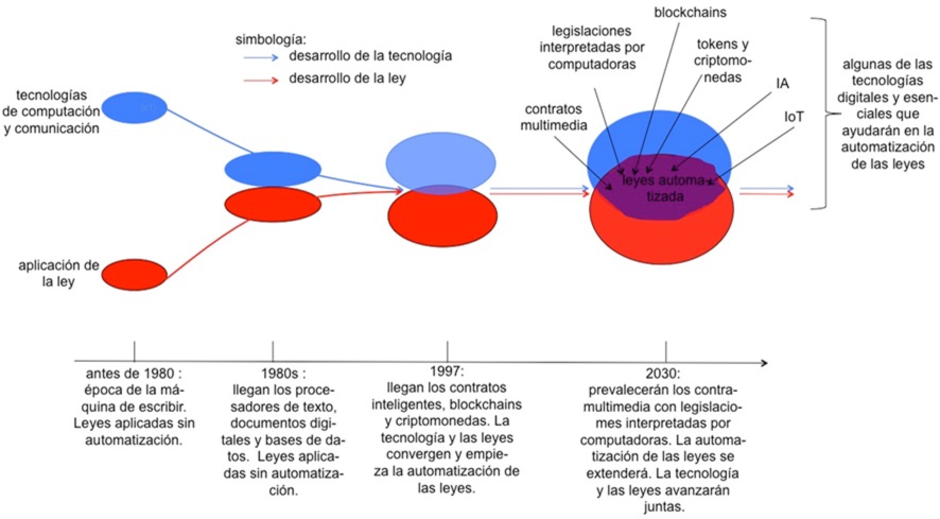
\includegraphics[width=1.0\columnwidth]{imagenes/convergencia.pdf}
\caption{Evolución de la convergencia entre el Derecho y la Tecnología.}
\label{fig:convergencia}
\end{figure}



As shown in Fig.~\ref{fig:sd}...

\begin{figure}
\centering

\includegraphics[width=0.45\columnwidth]{imagenes/SnowDrop30Dec2022.pdf}
\caption{This fig is about a beautiful flower.}
\label{fig:sd}
\end{figure}



\section{Cross references}
Esto lo analizaremos en la Section~\ref{howtocite}...
y esto en Cap~\ref{goberalgoritmica}

\section{How to include citations}
\label{howtocite}

You need to include citatation ...

 
text text text


Una cita \cite{LawCommission2021}, otra cita

 

\cite{LawCommission2020} otra cita mas

\cite{LawCommissionSummary2020}


bla bla text



\cite{Samer2017}

\cite{PrimaveraAaron2018}


\cite{Andersson2020}


%% carlos: https://www.overleaf.com/learn/latex/Bibliography_management_with_biblatex
%%https://tex.stackexchange.com/questions/21439/is-there-any-advantage-to-using-addbibresource-over-bibliography

Ejemplos de cita de un libro \cite{Andersson2020} y 
de un articulo \cite{Samer2017}.



 
\subsection{How to add numbered lists}

You can make lists with automatic numbering \dots

\begin{enumerate}
  \item rrrrrr.
  \item    soy sd.
  \item and like this.
\end{enumerate}


\subsection{How to add bullet lists}

\begin{itemize}
 \item Like this,
 \item and like this.
\end{itemize}


\subsection{How to add description lists}

\begin{description}
 \item[apples] are nice. \textbf{negritas} \textit{italics}.
 \item[grapes] are sweet.
\end{description}


\subsection{How to include Figures}
First you have to upload the image file from your computer using the upload link in the file-tree menu.  

Note that your figure will automatically be placed in the most appropriate place for it, given the surrounding text and taking into account other figures or tables that may be close by. You can find out more about adding images to your documents in this help article on \href{https://www.overleaf.com/learn/how-to/Including_images_on_Overleaf}{including images on Overleaf}.
 

\subsection{How to add Tables}

Use the table and tabular environments for basic tables  



\begin{table}
\centering
\begin{tabular}{l|r}

Item & Quantity \\
\hline

Widgets & 42 \\

Gadgets & 13
\end{tabular}
\caption{\label{tab:widgets}An example table.}
\end{table}





\section{Resumen}

En esta tesis estudiamos las implicancias jurídicas de la automatización de las leyes, más conocida en
la actualidad como \textbf{gobernanza algorítmica}. Todo ello en el contexto de sistemas descentralizados, es decir
aquellos sistemas que no se encuentran bajo el control de una sola autoridad \textit{(peer-ro-peer)}. Muchas e
innovadoras son las ventajas que la automatización y la descentralización brindan a quienes la utilizan.
Desafortunadamente, también ocasionan enormes desafíos técnicos y jurídicos. Esta tesis está enfocada en el
estudio de los últimos, pero con interés particular en la línea en donde las leyes y la tecnología digital
convergen. La contribución principal de este trabajo es el desglose del concepto de gobernanza algorítmica
dentro del contexto de las tecnologías digitales que están creando una sociedad en donde los modelos
económicos son cada día más descentralizados. Específicamente, la tesis identifica las lagunas jurídicas
que aquejan a la gobernanza algorítmica en el contexto de la descentralización. Para algunos interrogantes
propone soluciones y para otros, los ordena y presenta como temas abiertos de investigación. Es posible que
el aporte más relevante de este trabajo sean precisamente los temas abiertos de investigación que planteamos
y que contribuyen con la \textbf{automatización de las leyes}. Este concepto se basa en varios de los términos
técnicos que estudiamos en profundidad y hoy en día es uno de los motivos de análisis de mayor interés. La
razón principal de su relevancia radica en la estrecha vinculación con ideas innovadoras tales como, las
criptomonedas, la economía tokenizada, las finanzas descentralizadas,la inteligencia artificial, Internet de las cosas (IoT), los gobiernos descentralizados y la identidad digital. Sin duda está investigación permitirá avanzar en
un aspecto importante del conocimiento jurídico. El Derecho no puede desconocer las innovaciones que
surgieron particularmente en la última década y que, además, se están empleando en distintas áreas de la
sociedad.

\textbf{Palabras clave:} gobernanza algorítmica, leyes automáticas, smart contracts, descentralización, identidad digital



\chapter{Introduction}
\label{Introducción}
% Start writing here----------------------------------------------------
La gobernanza algorítmica y las estructuras descentralizadas, temas centrales de esta tesis, se basan en la virtualidad, lo que significa que no podrían existir sin internet. Por esta razón, consideramos conveniente dedicar este capítulo a aclarar algunos conceptos técnicos que pueden llegar a generar dudas o mal entendimiento en los contenidos de los sucesivos capítulos. En las próximas secciones dedicaremos unos párrafos para explicar la evolución de Internet y, de esta manera, poder comprender su posterior crecimiento. Luego, analizaremos su funcionamiento e intentaremos dilucidar ciertas cuestiones que aún, en la actualidad, no se encuentran claras como, por ejemplo, quiénes son los propietarios de esta red mundial, cómo es su arquitectura y cuáles son las implicancias jurídicas más relevantes.





\chapter{Tecnología para la Gobernanza Algorítmica}
\label{Tecnología para la Gobernanza Algorítmica}
\section{Introducción}
La gobernanza algorítmica y las estructuras descentralizadas, temas centrales de esta tesis, se basan en la virtualidad, lo que significa que no podrían existir sin internet. Por esta razón, consideramos conveniente dedicar este capítulo a aclarar algunos conceptos técnicos que pueden llegar a generar dudas o mal entendimiento en los contenidos de los sucesivos capítulos. En las próximas secciones dedicaremos unos párrafos para explicar la evolución de Internet y, de esta manera, poder comprender su posterior crecimiento. Luego, analizaremos su funcionamiento e intentaremos dilucidar ciertas cuestiones que aún, en la actualidad, no se encuentran claras, como por ejemplo, quienes son los propietarios de esta red mundial, cómo es su arquitectura y cuáles son las implicancias jurídicas más relevantes.

\subsection{Principios de Internet}
Muchas fueron las expectativas y aspiraciones que acompañaron el desarrollo de Internet. Su gobernanza se puso en marcha a través de tres principios fundamentales:

\begin{enumerate}
  \item{\textbf{Principio “de punto final a punto final”}\textit{(end-to-end principle)}}  Este principio dictamina que una aplicación de Internet se instala en una computadora (por ejemplo, la PC de Mary) que se encuentra conectada a un ISP \footnote{ISP (siglas en inglés de Internet Service Provider), en informática, es el Proveedor de Servicios de Internet}  e interactúa con otras computadoras que también están conectadas a un ISP (por ejemplo, la PC de Peter). Ambas (tanto la PC de Mary como la de Peter) se comunican a través de la infraestructura que queda en medio, lo que los expertos llaman “la red” y se compone de varios ISPs que funcionan como simples tubos que transmiten el tráfico que intercambian las computadoras (en este caso de Mary y de Peter). Se denomina “simples tubos” debido a que los ruteadores \footnote{Un rúter, (router en inglés),  enrutador o encaminador es un dispositivo que permite interconectar redes con distinto prefijo en su dirección IP. Su función es la de establecer la mejor ruta que destinará a cada paquete de datos para llegar a la red y al dispositivo de destino}  no procesan información sino simplemente la transmiten.  En otras palabras, las aplicaciones se instalan siempre en computadoras que están fuera de los ISPs, nunca en alguno de los ruteadores R1, R2, R3, etc. Esta innovación ha sido uno de los grandes aciertos del diseño de Internet considerando que cualquier persona (diseñador) podría implementar una aplicación e introducirlo en una computadora que se encuentre conectada a la red (por ejemplo, una plataforma para crowdfunding para el arte). Cabe mencionar que a los ISPs que se encargan de transmitir los datos que la aplicación genera, no le afecta el tipo de aplicación.

\item{\textbf {Principio de red pública} \textit{(Permissionless innovation principle):}} Este principio determina que cualquier persona física o jurídica (empresa) tiene derecho a inventar una aplicación e instalarla en una computadora conectada a Internet (por ejemplo, la PC de Alice, Mary o Peter) sin tener que pedir permiso a nadie. No existen obstáculos legales para instalar nuevas aplicaciones. Tampoco hay necesidad de pedirle autorización a los ISPs que transmitirán el tráfico (datos) generado o recibido por la nueva aplicación.  El único requisito es ajustarse a los estándares técnicos de Internet. Por ejemplo, utilizar los protocolos de Internet que permite el funcionamiento: el TCP/IP hace funcionar a los ISPs, el HTML a las páginas web \footnote{Las páginas web fueron inventadas por Tim Berners—Lee in 1989. Para más información véase: https://webfoundation.org/about/vision/history-of-the-web/} , y el SMTP al email; si la aplicación no sigue estos protocolos, simplemente no funcionaria, pero no afectaría a los ISPs. Este principio ha sido una de los grandes aciertos para promover la innovación en Internet; podemos decir que internet funciona de manera descentralizada. Este tema lo retomamos en el capítulo \ref {Descentralización} en donde analizamos el grado de descentralización de la Red, en la práctica. Es importante destacar que, gracias a este principio, han surgido muchos inventos que usamos cotidianamente, como por ejemplo las páginas web. Una de las creaciones más recientes y que nos interesa en esta tesis son las blockchains. Por este principio, cualquier individuo de cualquier parte del mundo, puede instalar y utilizar en su computadora conectada a Internet, la plataforma Blockchain. A modo de ilustración podría pagar con bitcoin en la plataforma de Bitcoin o participar como minero. Esto lo analizaremos en profundidad en la Seccion \ref{Blockchain} del capítulo Descentralización. Por otro lado, debido a su condición de red pública, Internet es un espacio no regulado, lo que ha generado grandes problemas jurídicos como fraudes, tráfico de pornografía y otros temas relacionados con la publicación de datos personales y el derecho al olvido.

\item{\textbf {Principio de red abierta}\textit{ (Openess principle):}} Este principio dice que la transmisión de datos a través de los ISPs es abierta, es decir, sin restricciones jurídicas. .[2] El trabajo de los ISPs es funcionar como medio de transmisión de datos (simples tubos) sin importar su contenido. Los ISPs no tienen derecho a seleccionar los datos (transmitir unos y otros no), ni siquiera tienen el derecho de inspeccionarlos.  Por este principio, los usuarios de Internet tienen la seguridad de que lo que ellos envíen a otro usuario, será recibido tal cual lo remitieron. Asimismo, los usuarios de Internet tienen garantizado que los ISPs no inspeccionarán ni almacenarán sus datos. Por ejemplo, en la Fig. 1, ninguna red (2,3, 5,7) tiene facultad para almacenar el mensaje que Alice envía a Peter. Las únicas computadoras que pueden hacerlo son la emisora (la PC de Alice) y la receptora (la PC de Peter).

\end{enumerate}

En la actualidad, la red no es la misma de la década de los ´90, en donde los usuarios navegaban principalmente para acceder a sus correos electrónicos y buscar información. Ahora, se han incorporado numerosas aplicaciones y funciones para una gran cantidad de usos, tal es el caso del comercio electrónico, la educación en línea o el financiamiento a través de Internet. Además, la red actual tiende a una concentración y descentralización. En el 2009 el 50\% del tráfico estaba a cargo de 150 intermediarios. En 2013 son sólo 35 empresas las que trafican ese mismo 50\%. A la vez, aparece un creciente interés de los gobiernos por controlar los contenidos que por allí circulan.

Internet es hasta cierto punto un sistema descentralizado, si bien no lo es totalmente debido a que en la actualidad se podría decir que la controlan algunas pocas empresas (oligopolio)[3] y organizaciones como IETF o Web Consortium que imponen sus reglas. 

La falta de regulación legal sumado al \textit{“openess principle”}, (a través del cual los ISPs no necesitan ver el contenido de los mensajes sino solo el encabezado: nombre, dirección del destinatario), hacen que si el emisor envía un mensaje encriptado al recipiendario solamente ellos conocerán su contenido. Los gobiernos no siempre están de acuerdo con este principio porque no pueden colocar \textit{“wire\-taps”} (escucha o intervención telefónica) en los ruteadores de los ISPs para conocer el cuerpo de los mensajes.

De estos principios surgen implicancias jurídicas que afectan a la gobernanza algorítmica que veremos en próximas secciones de este capítulo. 

\section{Breve historia de Internet}

Internet se ha convertido en un fenómeno tecnológico que causó un gran impacto en la sociedad, y en el mundo. Fue el resultado del pensamiento visionario de personas que a principios de la década de 1960, vieron un valor potencial al permitir que las computadoras compartieran información sobre investigación y desarrollo en los campos científico y militar. En 1962, CR Licklider[4] (MIT) propuso por primera vez una red global de computadoras, mientras que Leonard Kleinrock (MIT) desarrolló la teoría de la conmutación de paquetes, que iba a formar la base de las conexiones a Internet. Por otro lado, Lawrence Roberts (MIT) conectó una computadora de Massachusetts con otra de California en 1965, a través de líneas de acceso telefónico. Internet, entonces conocida como ARPANET, se puso en línea en 1969 bajo un contrato otorgado por la Agencia de Proyectos de Investigación Avanzada (ARPA) que inicialmente conectó cuatro computadoras de universidades en el suroeste de los EE. UU. La primera Internet fue utilizada por expertos en informática, ingenieros, científicos y bibliotecarios que tenían que aprender a usar un sistema muy complejo. En aquellos días no había computadoras personales en el hogar, ni en la oficina.

Otro importante avance se produce con la incorporación del correo electrónico.  En 1972,  Ray Tomlinson \footnote{Escogió el símbolo @ de los símbolos disponibles en su teletipo para vincular el nombre de usuario y la dirección.}  de BBN, lo adaptó para ARPANET. El cambio fundamental hacia una Internet de base comercial se origina con la entrada a gran escala de Microsoft en el mercado de navegadores, servidores y proveedores de servicios. World Wide Web es una de las innovaciones más relevantes. Se trata de una plataforma que facilita el acceso a los datos en Internet. Utiliza enlaces de hipertexto que son fragmentos de código que vinculan un sitio a otro (y en muchos casos un host de computadora a otro host de computadora). Si bien fue el navegador lo que hizo posible y fácil ver las páginas web de manera simple y rápida, se necesitaban otros componentes para navegar por la web. Por ejemplo, la web estaba creciendo tan rápido que era difícil hacer un seguimiento de lo que contenía. Lo que se necesitaba era un directorio. Con tanta información en la web a principios de la década de 1990, muchos intentaron encontrar una forma de buscar fácilmente esta información y recuperarla. La solución a este problema fue el motor de búsqueda como Yahoo o Google. Durante gran parte de la década de 1990, muchos hogares vieron Internet como una tecnología extranjera que no era tan simple de usar. Sin embargo, AOL (America Online) se centró en estos nuevos usuarios no técnicos. A lo largo de los años, AOL tuvo una enorme influencia en la introducción de muchos servicios web a las masas, incluidos correo electrónico, salas de chat, mensajería instantánea, entre otros.

Durante este período de enorme crecimiento, las empresas que ingresaron al ámbito de Internet se apresuraron por encontrar modelos económicos que funcionaran. Los servicios gratuitos respaldados por publicidad desplazaron algunos de los costos directos del consumidor, al menos temporalmente [5]. Las ventas en línea se desarrollaron rápidamente para productos como libros, CD de música y computadoras, a pesar que los márgenes de ganancia eran relativamente escasos. Los modelos de negocio que han funcionado bien eran los portales, que intentaron ofrecer una variedad de artículos y servicios a un público amplio. La adquisición de Time-Warner por parte de AOL fue la fusión más grande de la historia y muestra el enorme crecimiento del negocio de Internet. El mercado de valores tuvo altibajos al igual que las nuevas empresas de tecnología. La disminución de los ingresos por publicidad supuso el quiebre de muchas empresas “punto.com”, y las que subsistieron tuvieron que reorganizarse y buscar mejores modelos de negocio.

Una tendencia actual con importantes implicaciones para el futuro es el aumento de las conexiones de alta velocidad. La tecnología inalámbrica ha crecido rápidamente en los últimos años y los viajeros buscan zonas de wi-fi donde pueden conectarse mientras están fuera de su casa u oficina. Muchos aeropuertos, cafeterías, hoteles y shoppings brindan estos servicios de manera rutinaria, algunos por una tarifa y otros de forma gratuita. Un área de gran desarrollo al presente es el aumento hacia el acceso inalámbrico universal. Asimismo, se evidencia un avance importante hacia dispositivos de menor tamaño para conectarse a Internet. Las tabletas, los teléfonos inteligentes, los libros electrónicos, las máquinas de juego, los relojes de pulsera, los dispositivos GPS, los termostatos e incluso las bombillas ahora pueden acceder a la web. El Internet de las cosas (IoT) también está agregando dispositivos (televisores modernos, automóviles, cámaras, reemplazos de taxis, drones, auriculares de realidad virtual y más artículos y servicios).

A medida que Internet se vuelve omnipresente, más rápido y cada vez más accesible es para las comunidades no técnicas, las redes sociales y los servicios de colaboración. Un motivo esencial es que Internet permite a las personas comunicarse y compartir intereses de muchas formas. Sitios como Facebook, Twitter, Linked-In, Flickr, Second Life, blogs, Instagram, wikis y muchos más hacen posible que personas de todas las edades compartan rápidamente sus intereses del momento con otros en todas partes. Al mismo tiempo crece la necesidad de proteger la privacidad convirtiéndose en un enorme desafío para los responsables de crear las leyes.


La historia de Internet no estaría completa si np se menciona las numerosas aplicaciones que impulsaron su crecimiento. A lo largo de los años, muchas aplicaciones e innovaciones han hecho de Internet, y específicamente de la World Wide Web, un destino no solo para las personas, sino también para las empresas. 

No se puede decir lo suficiente sobre el impacto económico que Internet ha traído al mundo. Quizás se han creado billones de dólares en riqueza a partir de Internet y se han cambiado miles de millones de vidas debido al comercio electrónico.

A lo largo de la década de 1990, gran parte del crecimiento de la economía mundial en general se atribuyó a las computadoras e Internet y continúa hasta el día de hoy. De hecho, la economía global se puede otorgar a muchas de las innovaciones de Internet. Con más y más población mundial capaz de hacer negocios en línea, los mercados mundiales están más entrelazados que nunca.

El mundo definitivamente ha cambiado debido a la capacidad de Internet para comunicarse con facilidad desde prácticamente cualquier lugar. En unas pocas décadas, Internet ha pasado de ser una red de unas pocas docenas de computadoras a conectar prácticamente a toda la población mundial. 

\section{Internet, arquitectura y funcionamiento}


 
\begin{figure}
\centering
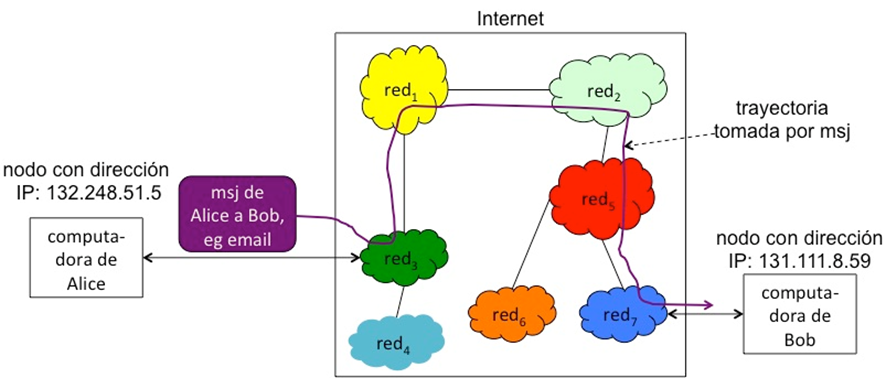
\includegraphics[width=0.85\columnwidth]{imagenes/enviomsjAlice2Bob.png}
\caption{Envio de un mensaje de email por Internet}
\label{fig:enviomsjAlice2Bob.png}
\end{figure} 



\subsection{La red de redes}

Internet es una red de redes. De ahí proviene el nombre. Es decir, Internet es un conjunto de cientos de redes interconectadas a las cuales se conectan computadoras que son capaces de enviar y recibir mensajes en formatos que sigan los estándares de Internet. La Figura \ref{fig:enviomsjAlice2Bob.png} muestra un diagrama simplificado de Internet que presenta únicamente siete redes y dos computadoras. Como se indica en la figura, las computadoras que se conectan a la red se  llaman “nodos”. Es un nombre genérico que se utiliza para referirse a cualquier dispositivo que se conecta a Internet. Otros ejemplos de dispositivos son las supercomputadoras, las tabletas, los teléfonos celulares y los dispositivos IoT.

Con el fin de poder conectarse entre sí, a cada dispositivo se le asigna una dirección, conocida como “dirección IP” que permitirá a una computadora (por ejemplo, la de Alice), especificar la dirección del destinatario de un mensaje; en este caso es la 131.111.8.59. Estas direcciones son numéricas y muy fáciles de manejar a nivel de programación, pero muy difíciles de recordar para el ser humano. A fin de evitar estas dificultades, los ingenieros de software mapean (convierten) estas direcciones numéricas en otras equivalentes que son más intuitivas. De esta manera, una persona (Alice) puede escribir el nombre del destinatario como bob@rainland.com,  en lugar de 131.111.8.59.

En la ilustración que estamos analizando, se muestra que el mensaje que Alice envía a Bob es un email, pero de igual forma podría ser un mensaje de WhatsApp o cualquier otra aplicación. Lo importante es que dicho mensaje viaja por la red de redes a través de algunos de los caminos posibles (hay varios), hasta llegar al destinatario.

Ante esta situación, surge la siguiente pregunta: ¿dónde se localizan geográficamente la red?  ¿A quiénes pertenecen? Este interrogante es importante por las implicaciones jurídicas a las que se encuentran expuestos los usuarios de Internet cuando hacen uso de ella. Por ejemplo, cuando realizan operaciones comerciales en línea.

Para identificar las consecuencias legales, es primordial entender la arquitectura (anatomía) de Internet a nivel administrativo. La figura \ref{fig:InerneteISP} que analizaremos en las siguientes secciones, muestra una visión simplificada de  Internet al presente (teniendo en cuenta que se trata de un sistema que está en constante evolución). La arquitectura ilustrada es distinta de aquella Internet de los años 80s cuando los teléfonos celulares inteligentes no estaban en el mercado, y seguramente será obsoleta dentro de 15 o 20 años cuando surjan nuevos dispositivos y aplicaciones que en la actualidad difícilmente nos podemos imaginar.


\begin{figure}
\centering
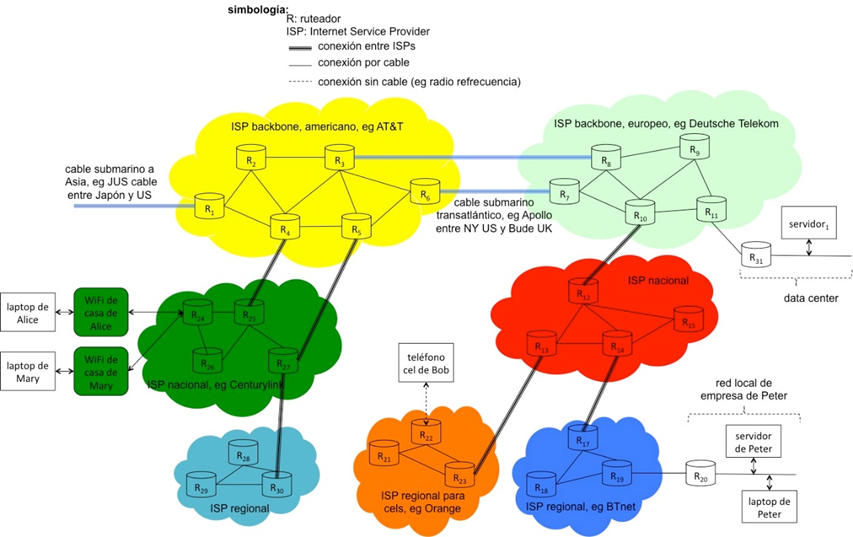
\includegraphics[width=0.85\columnwidth]{imagenes/cabrablanca.png}
\caption{La Internet: red de ISP independientes.}
\label{fig:InerneteISP}
\end{figure} 

\subsubsection{La red de redes de ISP independientes}

En la Figura \ref{fig:InerneteISP}, Internet puede verse como un conjunto de redes que pertenecen a diferentes empresas de comunicaciones y por ende, son administrativamente hablando, autónomas. A estas empresas se las conoce como Proveedores de Servicio de Internet \textit{(Internet Service Providers )} o ISP . La figura \ref{fig:InerneteISP} muestra siete ISPs.

No profundizaremos en la estructura interna de estas redes, basta entender que se componen de cables y computadoras interconectadas. Estas computadoras transmiten datos y se conocen como ruteadores. La figura muestra algunos: R1, R2, R3, etc.  La misión de los ruteadores es recibir un mensaje, escoger una ruta de las disponibles para hacer llegar el mensaje al destinatario y reenviar el mensaje por la ruta seleccionada. Como se observa en la figura, los ruteadores funcionan como puentes que unen varios caminos. Por ejemplo, lo normal es que un mensaje enviado por una persona de una empresa de New York, a una persona de una empresa en Cambridge, pase por varios ruteadores antes de llegar a su destino y que, a su vez, en el camino haya diferentes opciones (rutas) para llegar al punto final.

\section{Proveedores de Servicios de Internet \textit{(Internet Service Providers} o ISP)}

Un ISP es una empresa que vende servicios de comunicación de datos o acceso a Internet. Algunos ISPs se dedican a transmitir grandes volúmenes de datos entre puntos geográficamente distantes, mientras que otros se dedican a conectar a los consumidores (empresas, casas, etc.) a Internet.

La característica principal de un ISP, desde el punto de vista de la administración, es la de ser una empresa independiente y competir con otras que ofrecen servicios similares. Debido a esto, los ISPs también se conocen como Sistemas Autónomos \textit{(Autonmous Systems or ASs)}. 

En esta tesis, nosotros usaremos el término ISP en lugar de AS, en concordancia con el libro de Andrew Tanembaum\footnote{Tanenbaum, Andrew S., Wetherall, David J., “Computer Networks”, Fifth, Prentice Hall, 2011. páginas 62 y 432}  –uno de los autores más conocidos en este tema y en cuyo libro hemos basado la figura.

Internet no tiene una arquitectura (anatomía) bien definida. Sin embargo, existe una jerarquía en donde unos ISPs dependen de otros para proporcionar  su servicio. Estas dependencias están regidas por acuerdos comerciales entre los ISPs en donde se compra, vende e intercambia servicios.


\section{Columna vertebral \textit{ (ISP backbones)}}

La Figura \ref{fig:InerneteISP} muestra dos ISP de los llamados “columna vertebral”
 \textit{(backbones)} (llamados ISP de Tier 1): uno, americano (AT\&A) y el otro, europeo (Deutsche Telekom).  Existen otros, entre ellos CenturyLink, Cogent Communications, Global Telecom and Technology (GTT), NTT Communications, Sprint, Tata Communications, Telecom Italia Sparkle, Telia Carrier, and Verizon[2]. El negocio de estas compañías es la transmisión de grandes volúmenes de datos entre largas distancias. Debido a esta función, forman la columna vertebral de Internet. Como se observa en la Figura mencionada al comienzo de este párrafo, los llamados ISP nacionales[3] se conectan a los ISPs que forman la columna vertebral de Internet (este servicio no es gratuito), al igual que los llamados Centro de datos (Data center) que buscan grandes velocidades de transmisión de datos.

Los ISPs se enfocan en la transmisión de datos, Por esta razón, también se los denominan \textit{“Network Service Providers”} (NSP)[4]. Esto se debe a que a la transmisión de datos se la conoce como servicio de red puesto que funciona solo como un “tubo”, por el que circulan datos sin importar el contenido y sin ser procesados: nadie (persona o computadora) analiza el contenido, el análisis del contenido es la responsabilidad y privilegio solamente del destinatario.

\subsection{ISP nacionales}

Los ISP nacionales reciben este nombre porque suelen tener presencia en todo un país, por ejemplo, en todos los estados de Estados Unidos. Sin embargo, no significa que sean únicos; por el contrario, compiten con otros ISPs nacionales. El negocio de los ISPs nacionales es vender transmisión de datos a otros ISPs como los ISPs regionales.  Es necesario no perder de vista que existe una estructura jerárquica.

Algunos ISPs nacionales también ofrecen conexión a Internet a los usuarios. La figura muestra como ejemplo, al ISP nacional Centurylink (color verde) que además de vender conexión a Internet a usuarios como Alice y Mary, vende transmisión de datos a ISPs regionales.

Por su parte, en un sistema descentralizado no existen reglas estrictas sino que se rige por la oferta y la demanda.

\subsection{ISP regionales}

Los ISPs regionales (llamados ISP de Tier 3) se dedican al negocio de la conexión de usuarios a Internet, como casas y empresas.  Son los más conocidos para los usuarios puesto que conectan las casas a Internet a través de Wifi.  La figura muestra el ejemplo del ISP regional BTnet, Estos ISPs también conectan empresas. Se llaman regionales porque suelen ser empresas pequeñas que se enfocan en vender sus servicios en regiones específicas de un país.

En esta estructura relativamente jerárquica, los ISPs regionales dependen de los servicios de transmisión de datos que venden los ISPs nacionales, e indirectamente, de los servicios de transmisión de datos que venden los ISPs de la columna vertebral (ISP backbones). Por ejemplo, obsérvese que en la Figura\ref{fig:InerneteISP} los ISPs regionales Orange y BTnet dependen del ISP nacional de color rojo para transmitir sus datos. En este caso, Bob nunca podría recibir un mensaje de Alice (conectada al ISP de color verde) si el ISP nacional de color rojo, no le entrega el mensaje a Alice. Naturalmente, el ISP nacional (rojo) depende de los servicios de transmisión de datos de AT\&T y éste de los servicios de transmisión de datos de Deutsche Telekom.

\subsection{Distintas tecnologías para el uso de Internet}

A un nivel más técnico, Internet puede verse como un conjunto de hardware y software basados en varias tecnologías. Mencionaremos solo algunas como base para entender las figuras que usamos en otros capítulos. Aclaramos, sin embargo, que estos detalles no son cruciales para este trabajo de tesis.

La tecnología para conectar un dispositivo a Internet o un ISP con otros, es variada. La figura \ref{fig:InerneteISP} muestra la conexión por cable y la conexión sin cable. En la conexión por cable se usa alambre de cobre torcido (el que vemos llegar a nuestras casas), cables coaxiales y fibra óptica. En la conexión sin cable es, por citar un ejemplo, la tecnología de radio frecuencia con la que trabajan nuestros teléfonos celulares y el Wifi que tenemos en nuestras casas. Otro ejemplo, es la tecnología de los satélites espaciales y la de Bluetooth que usamos para conectar nuestro ratón y teclado inalámbrico a nuestra laptop.

\subsection{Jurisdicciones}

Es necesario tener presente que, en relación con la ubicación geográfica de los ISPs de la figura, los mismos suelen expandirse a lo largo de regiones, estados, países y continentes, es decir, abarcan varias jurisdicciones.  Otra observación importante es que, los ISPs ilustrados en las figuras, son solamente la infraestructura (la base) de comunicación sobre la que se instalan las aplicaciones con las que nosotros, los usuarios interactuamos diariamente: las páginas web que visitamos, email, WhatsApp, Facebook, Twitter, YouTube, Amazon, eBay, acceso a bancos y desde luego, las plataformas de crowdfunding y las blockchains como Bitcoin, Ethereum y la Hyperledger.

El alcance internacional de Internet lo resaltan los cables submarinos que hemos incluido en la figura. Por ejemplo, el cable Apollo (aclaramos que hay docenas de ellos) que conecta Nueva York con la ciudad de Bude, en Gran Bretaña, une física y lógicamente dos países y dos continentes. Por ese cable se transmiten datos de varios países, muchos de estos datos son confidenciales: datos personales, datos de valor comercial y secretos de Estado. Adviértase que muchas veces, Estados Unidos y Gran Bretaña no son los destinos finales de dichos datos, aquellos pueden estar destinados a otros países, como pueden ser Alemania o Canadá.\footnote{HMN Technologies, “Submarine cable map”, https://www.submarinecablemap.com}   

\subsection{Esquema de representación de Internet}

La Figura \ref{fig:InerneteISP} muestra algunos detalles del funcionamiento interno de Internet. Cuando dicho funcionamiento interno ya está claro, es conveniente eliminar los detalles y pasar a una representación simple. De manera simplificada, los expertos suelen representar a Internet como se indica en la Figura \ref{figrepresentaciondeinternetnubes}, es decir, a través de una nube donde no se encuentran los ruteadores de los ISPs. Incluso suele sustituirse por una sola nube en lugar de seis como se detalla en la Figura \ref{fig:representaciondeinternetunanube}. 



\begin{figure}
\centering
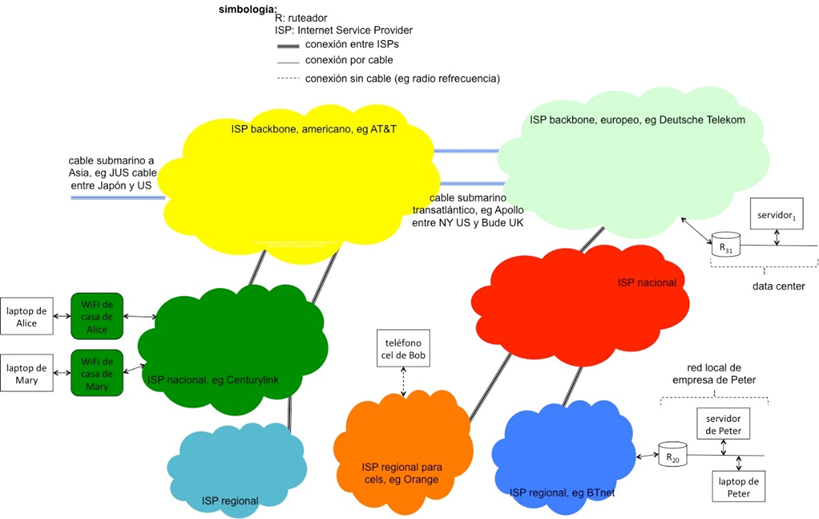
\includegraphics[width=0.85\columnwidth]{imagenes/toroloco.png}
\caption{Representation de Internet.}
\label{figrepresentaciondeinternetnubes}
\end{figure} 


\begin{figure}
\centering
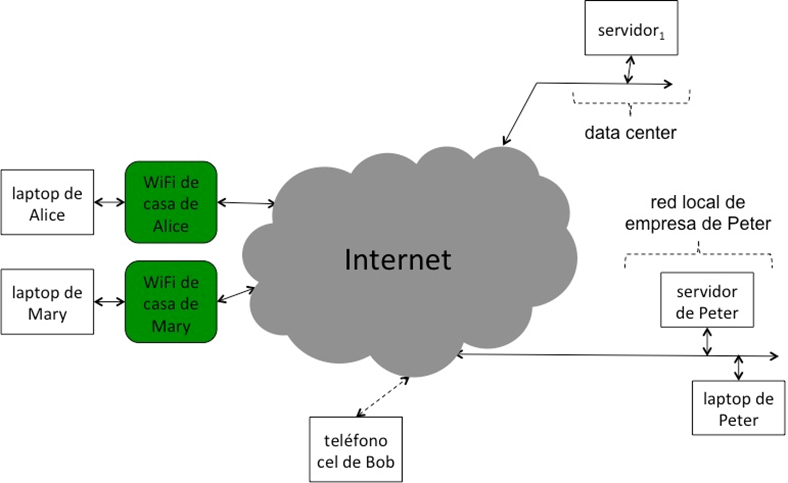
\includegraphics[width=0.85\columnwidth]{imagenes/pezplata.png}
\caption{Representación de Internet a través de una sola nube.}
\label{fig:representaciondeinternetunanube}
\end{figure} 


\begin{figure}
\centering
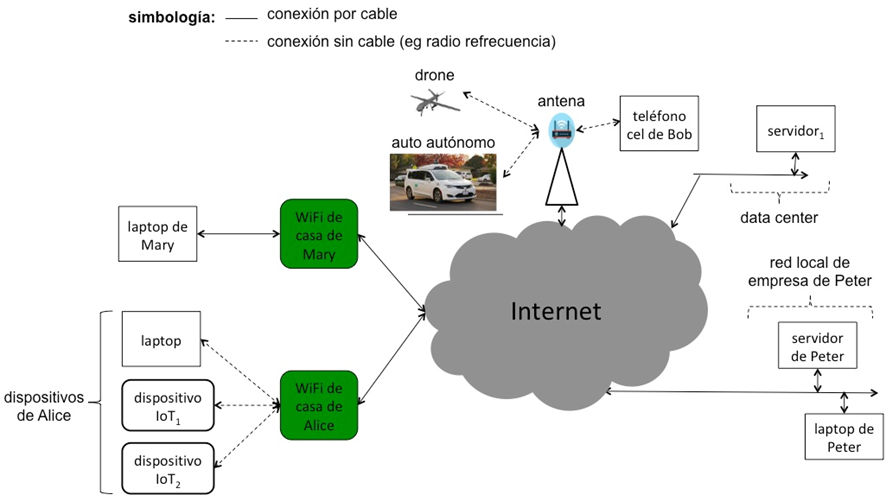
\includegraphics[width=0.98\columnwidth]{imagenes/IoTinternetautodrone.png}
\caption{Internet con auto automáticco, drone y dispositivos IoT domésticos.}
\label{fig:IoTinternetautoautodrone}
\end{figure} 



\subsection{Ecosistema de Internet}

Las organizaciones y comunidades que ayudan a Internet a funcionar y evolucionar se denominan \textbf{Ecosistema de Internet}. Comparten valores comunes para el desarrollo abierto de Internet.[1] El rápido y continuo avance, así como la adopción de tecnologías se puede atribuir a la participación de organizaciones que componen el ecosistema de Internet tales como


\textbf{Tecnólogos, ingenieros, arquitectos, creadores y organizaciones} como el  Grupo de trabajo de ingeniería de Internet y el  Consorcio World Wide Web, que ayudan a coordinar e implementar estándares abiertos.

\textbf{Organizaciones globales y locales} que gestionan recursos para el direccionamiento global. Entre ellos se encuentran la  Corporación de Internet para la Asignación de Nombres y Números, que incluye la Autoridad de Números Asignados de Internet, los Registros Regionales de Internet y los Registros y Registradores de Nombres de Dominio.

\textbf{ Operadores, ingenieros y proveedores} que brindan servicios de infraestructura de red, como proveedores de servicios de nombres de dominio, operadores de red y puntos de intercambio de Internet.

\textbf{Usuarios de Internet} que utilizan Internet para comunicarse entre sí y ofrecer servicios.

\textbf{Educadores} que enseñan y ayudan a desarrollar y usar tecnologías de Internet, como organizaciones multilaterales, instituciones educativas y agencias gubernamentales.

\textbf{Responsables de políticas y toma de decisiones} que se ocupan del desarrollo y la gobernanza de políticas locales y globales.


Entre los organismos más relevantes encontramos a la \textit{Internet Corporation for Assigned Names and Numbers} (ICANN) que es un organismo multisectorial creado en 1998 y organizado en base a comunidades de asesores y unidades de soporte sobre la asignación de DNS \textit{(Domain Name System)}, tarea que hasta el momento desarrollaban las universidades. Otro ámbito importante es el \textbf{Internet Governance Forum}  que consiste en un espacio de diálogo multisectorial sobre políticas, convocado por el Secretario General de Naciones Unidas en 2006 para “promover la seguridad, solidez y desarrollo de Internet”. Por otro lado, \textit{Internet Engineering Task Force}  (IETF)\footnote{https://www.ietf.org/about/who/
https://www.internetsociety.org
}  es un grupo de trabajo de ingeniería de Internet. Es abierto y accesible, tiene una labor técnica en la definición de los protocolos. Se trata de una gran comunidad internacional de diseñadores de redes, operadores, proveedores e investigadores preocupados por el desarrollo y buen funcionamiento de la arquitectura de Internet. La misión del IETF es hacer que Internet funcione mejor mediante la producción de documentos técnicos relevantes y de alta calidad que influyan en la forma en que las personas diseñan, utilizan y gestionan Internet.[3]

Internet funciona porque los estándares abiertos permiten que todas las redes se conecten entre sí. Esto hace posible que cualquier persona cree contenido, ofrezca servicios y venda productos sin requerir el permiso de una autoridad central. A diferencia de la red telefónica, que durante años en la mayoría de los países estuvo a cargo de una sola empresa, Internet global consta de decenas de miles de redes interconectadas gestionadas por proveedores de servicios, empresas individuales, universidades, gobiernos y otros.

\subsection{Internet en Argentina}

Internet en Argentina comenzó su desarrollo en la década de 1980, y su comercialización al público general se remonta a 1995, cuando se vendieron las primeras conexiones a Internet en el país. El dominio de nivel superior en la Argentina es .ar.

En el año 1985, se creó el Departamento de Computación de la Facultad de Ciencias Exactas y Naturales (FCEN) de la Universidad de Buenos Aires (UBA) donde un grupo de profesores, graduados y estudiantes comenzaron a trabajar en la investigación y el desarrollo de redes.  A comienzos de 1987, se logró establecer una conexión con la Universidad de Toronto de manera telefónica. Esta fue la primera comunicación internacional del país por correo electrónico, vía el protocolo UUCP. Paulatinamente, Argentina llegó a contar con más de 800 instituciones conectadas a través de correo electrónico.

Al mismo tiempo, en el año 1986 estaba en marcha el proyecto RUTA (Red Universitaria Teleinformática Argentina). Este proyecto proponía la interconexión de los centros de cómputos de varias Universidades Nacionales. Se trataba de una extensión de la propuesta original que había hecho la empresa IBM Argentina en 1984 de equipar estas instituciones con 
equipos \textit{mainframes}\footnote{ \url{https://es.wikipedia.org/wiki/Unidad_central}}. 

La modalidad de conexión basada en BITNET no tuvo continuidad en Argentina a causa de que internet se impuso como modelo a seguir y era más sencillo hacer crecer la red utilizando PCs como nodos de correo electrónico.

En 1994, la fundación de NIC Argentina comenzó a funcionar como organismo reglamentado y con las facultades para el registro de los dominios ‘.ar’. Al año siguiente, Internet se abrió al ámbito comercial logrando libre acceso a la comunidad en general. Dos años más tarde, se lanzan las primeras conexiones de banda ancha en la Argentina.9 El primer proveedor en comercializar este servicio en el país fue Fibertel.


En 2003, la banda ancha comenzó a avanzar de manera sostenida como modalidad preferida de acceso por parte de los usuarios. En ese año, la cantidad de abonados a internet de banda ancha creció un 35\%, al pasar de aproximadamente 150 000 en 2002, a más de 203 000 hacia finales de ese año. En 2013, el 100\% del mercado de conectividad en la Argentina correspondía a esa tecnología en sus diversas 
modalidades\footnote{\url{https://es.wikipedia.org/wiki/Internet_en_la_Argentina\#cite_note-10}} Además, Argentina mantiene conexiones de fibra óptica terrestres con países limítrofes.

%% 5 Jan 2023
%% 1) encierra cada link en  \url{} por ej https://www.cam.ac.uk
%% cambia a \url{https://www.cam.ac.uk}
%% 
%% 2) si la link contiene un % o un # debes de poner
%% \ a la izq del % y del #, por ej
%% \url{https://es.wikipedia.org/wiki/Internet_en_la_Argentina#cite_note-10}
%% ponlo \url{https://es.wikipedia.org/wiki/Internet_en_la_Argentina\#cite_note-10}
%%
%% Por ej \url{https://en.wikipedia.org/wiki/Mart%C3%ADn_Abadi}},
%% cambia a \url{https://en.wikipedia.org/wiki/Mart\%C3\%ADn_Abadi}
%%





Creemos importante mencionar que uno de los grandes expertos en seguridad computacional y en lenguaje de programación a nivel mundial es el argentino \textbf{Martín Abadi}~\footnote{Para más información véase: \url{https://en.wikipedia.org/wiki/Mart\%C3\%ADn\_Abadi}}, quien
junto con Hector Garcia Molina (Mex) y Ricardo Baeza (Chile) son los latinoamericanos que más han aportado al desarrollo de Internet.

%% Poner \ a la izq de % : carlos 5 Jan 2022


\subsection{Neutralidad de internet}

La neutralidad es un concepto difícil de definir: puede entenderse de diferentes maneras como por ejemplo que el tráfico debe ser tratado de la misma forma sin importar el origen. También como la garantía de acceso a cualquier sitio, sin discriminación e independiente del contenido, protocolo o plataforma.

El control en internet no tiene que ver sólo con cuestiones técnicas, aunque son muy importantes, se trata también de cuestiones políticas, a la que se suma el control que puedan querer ejercer los gobiernos.

Chile tiene una ley de neutralidad de la red. “La neutralidad de internet como norma jurídica es importante porque del principio se decanta el carácter abierto de la red y esto ha permitido el desarrollo de nuevos productos, servicios y modelos de negocios”. 

Existen argumentos en contra de la neutralidad que estipulan por ejemplo,  que el igual tratamiento obstruye los servicios diferenciados o que se afecta el normal desarrollo de los negocios y que, además, se pone en riesgo la seguridad y estabilidad de la red. 

\subsection{La regulación de Internet}

Hasta el presente, la regulación de Internet nunca ha alcanzado un espacio común internacional a pesar de ser la plataforma dominante para los individuos y las organizaciones que desean intercambiar información. Cada nación tiende a regular Internet según sus teorías fundamentales, perspectivas legales y diferencias culturales. 

Los beneficios económicos que generan las tecnologías emergentes son inmensos y ocasionan una transformación en las estructuras básicas de las economías de todo el mundo y alteraciones sustanciales dentro de las naciones. Además, producen implicancias jurídicas fundamentales como aquellas relativas a la privacidad y a la protección de datos, los derechos de propiedad intelectual y la regulación del contenido.
Estados Unidos, la Unión Europea (UE), Canadá y algunas áreas de Asia son los que más avances han logrado en tecnología y juegan un importante papel de liderazgo.\footnote{Bruce E. May, Jeng--Chung V. Chen, Kuang‐Wei Wen, “The differences of regulatory models and internet regulation in the European Union and the United States”, Information and Communications Technology Law, 13, 3}  

Las interacciones que se crean a causa de Internet trasciende las fronteras tradicionales de los estados-nación. La conformación de la identidad de una nación se ve influenciada debido a que Internet hace que sean permeables la cultura, las estructuras sociales, el idioma. Debido a estas transformaciones, los estados se ven obligados a explorar nuevos métodos y modelos de regulación. Sin embargo, no es una tarea fácil. Las diferencias culturales, políticas, sociales y económicas enraizadas en cada estado impactan en los enfoques y perspectivas de un nuevo orden normativo. El principal problema es la jurisdicción que históricamente estuvo determinada, en gran medida, por las fronteras geográficas  de cada Estado. Con Internet, ese poder jurisdiccional de los estados parece haberse limitado. Si bien es cierto que las señales electrónicas se originan y terminan desde una ubicación, pero la interacción real de la red se lleva a cabo en algún lugar allá afuera\footnote{  Bruce E. ib}  Se habla de “ciberespacio”, de “metaverso” (“más allá del universo”). La "ubicación" a menudo es imposible de determinar después que las señales se transfieren, mezclan, regeneran, cifran, desencriptan, alteran, modifican y mejoran. El ciberespacio es el lugar entre la transmisión y las terminales de recepción; el espacio indefinido donde dos seres humanos realmente se encuentran y se comunican.\footnote{Sterling, B., “Hacker Crackdown: Law and Disorder on the Electronic Frontie”r (New York, Bantam),1996} En este espacio ocurren innumerables transformaciones en todos los ámbitos de la vida de una persona. Por ejemplo, actividades comerciales, educativas, sociales, etc. La ubicación, a todos los efectos prácticos, ya no existe. La mayor preocupación es que las relaciones e interacciones ya no están teniendo lugar dentro de las fronteras de las sociedades tradicionales, sino que ocurren en el ciberespacio donde la ley se elude fácilmente. Este es el mayor inconveniente que los estados y los gobiernos deben atender y solucionar para protección de los derechos de las personas como miembro de la comunidad mundial.


\subsubsection{Modelos representativos de regulación de Internet}

Numerosas son las preguntas y desafíos que, como se dijo anteriormente, surgieron desde el nacimiento de Internet. Por ejemplo, se cuestiona si los sistemas legales previos a Internet funcionan para la regulación de la Red. El carácter no geográfico de Internet hace que sea muy difícil aplicar reglas territoriales a las actividades en línea, y los estados soberanos locales no pueden controlar las actividades en línea cuya ubicación física, muchas veces ni siquiera se puede establecer. La interacción entre las normas del espacio real – ley, normas sociales y fuerzas del mercado – y los del ciberespacio (código) son correspondientemente complejos. 

Algunos autores como David Johnson y David Post\footnote{Johnson, D.R. , Post, D.G.,  “And How Shall the Net Be Governed?” A Meditation on the Relative Virtues of Decentralized, Emergent Law. Unpublished paper, Temple University, 1996, \url{www.temple.edu/lawschool/dpost/writings.html} RecentWritings,  Johnson, D.R. , Post D.G., “Law and borders: The rise of law in cyberspace”, Stanford Law Review, 48, pp. 13–67.} , formularon modelos  básicos para la gobernanza de la red global que pueden resumirse de la siguiente manera:

%% aqui hay un prob con esa link. No existe: carlos 5 Jan 2023


\begin{enumerate}
  \item Los Estados soberanos territoriales pueden extender su jurisdicción, y reformar sus leyes según sea necesario, para intentar gobernar todas 
  las acciones en la red que tengan impactos sustanciales en sus habitantes. 
  
  \item Los Estados soberanos pueden celebrar acuerdos internacionales multilaterales para establecer reglas nuevas y uniformes específicamente aplicables a las conductas en la red. Sin embargo, los problemas con los tratados internacionales incluyen un proceso que es terriblemente lento, especialmente en contraste con el desarrollo extremadamente rápido de las nuevas tecnologías en Internet, los nuevos comportamientos y nuevos problemas de gobernanza.
  
  \item Una nueva organización internacional puede intentar establecer nuevas reglas, y nuevos medios para hacer cumplir esas reglas.

  \item Las reglas pueden surgir como resultado del complejo. La forma de acción colectiva propuesta implica una aceptación voluntaria de normas basadas en principios de derecho privado. Aquí se teoriza que “los protocolos técnicos de la red han creado un sistema adaptativo complejo que produce un tipo de orden que no se basa en decisiones judiciales, estatutos o votos”\footnote{Bruce E. May, Jeng--Chung V. Chen, Kuang‐Wei Wen, “The differences of regulatory models and internet regulation in the European Union and the United States”, Information and Communications Technology Law, 13, 3}.  
  
\end{enumerate}


Estos autores creen que Internet bien puede ser "gobernado" principalmente por el cuarto método, que ellos llaman "descentralizado, ley emergente”. La forma de acción colectiva propuesta implica un compromiso voluntario de aceptación de normas basadas en principios de derecho privado. 

Por su parte, Seifert\footnote{Siefert, J.W., “Who Will Protect Your Privacy?” Competing Rule Systems and the Regulation of
the Internet. Paper presented to the 41st Annual International Studies Association Convention, 2000.}  intenta capturar la gama de sistemas de reglas posibles en una escala de modelos de gobernanza de Internet o sistemas regulatorios que van desde aquellos altamente informales, como los mercados y la autorregulación, a sistemas de regulación muy centralizados, como el gobierno mundial. Seifert categorizó los rangos de Sistemas de reglas de Internet en cinco modelos. El primero, el Ciberespacio como Espacio Anárquico, en el extremo del sistema de regulación informal, ve Internet como un espacio separado con su propia autoridad. Este espacio está fuera de los límites territoriales del estado-nación y no está sujeto a la jurisdicción del estado. Este sistema de reglas informal extremo es el modelo propuesto por Johnson y Post en el cual el ciberespacio crea sus propias leyes e instituciones legales fuera de los límites territoriales del estado. El segundo, el Ciberespacio como Espacio Supranacional, está en el otro extremo. Este modelo incorpora la existencia de algún gobierno mundial que surge de los estados-nación y trata el ciberespacio como un espacio internacional para ser gobernado. El tercero, el Ciberespacio como Espacio Nacional, ve Internet como una tecnología que será regulada por las leyes nacionales. Este es el modelo defendido por muchos gobiernos nacionales. El cuarto, el Modelo de Régimen Internacional, prevé que los estados-nación firmen acuerdos de cooperación para abordar ciertos problemas o cuestiones como controles ambientales o cuestiones de derechos humanos. El último modelo, el modelo de Comunidad Epistémica, prevé el desarrollo de comunidades de conocimiento para crear políticas o influir en el proceso de formulación de políticas. Los responsables de formular y decidir sobre las políticas buscarían en estas comunidades información y orientación en las decisiones de política.


David Johnson y David Post \footnote{Johnson, D.R. , Post, D.G.,  “And How Shall the Net Be Governed?” A Meditation on the Relative Virtues of Decentralized, Emergent Law. Unpublished paper, Temple University, 1996, \url{www.temple.edu/lawschool/dpost/writings.html\#RecentWritings},  Johnson, D.R. , Post D.G., “Law and borders: The rise of law in cyberspace”, Stanford Law Review, 48, pp. 13–67.} expusieron una utopía ciberlibertaria, argumentando que la regulación sujeta a la soberanía estatal no podía funcionar en el ciberespacio, estableciendo que Internet era efectivamente no 
regulable.\footnote{Johnson, D.R. , Post, D.G.,  , ‘Law and Borders: The Rise of Law in Cyberspace’ (1996) 48 Stanford Law Review 1367 VER MICHELE
  Post, D., ‘Anarchy, State, and the Internet: An Essay on Making Law in Cyberspace’ (1995) Journal of Online Law art 3 accessed 28 February 2018.VER MICHELE}  Post, además, imaginó a Internet como una “opción de salida” de la jurisdicción territorial de los estados.\footnote{Esta Declaración señala no solo que la interferencia estatal era imposible.}  
  
  La Declaración de la Independencia del Ciberespacio fue la expresión más famosa de este movimiento.  El ciberlibertarismo culminó con la propuesta de un 'Estado de Internet', creado para evitar la interferencia de otros estados soberanos. La tierra escogida fue el Principado de Sealand, una isla fortaleza construida por las fuerzas militares británicas en aguas internacionales del Mar del Norte durante la Segunda Guerra Mundial\footnote{\url{https://sealandgov.org/}}.  Sealand fue poblada por una pequeña comunidad en 1967, que la declaró Estado independiente. En el año 2000 cypherpunks\footnote{Se conoce como cypherpunk a los activistas digitales que se focalizan en proteger la privacidad de los usuarios basándose en el uso de la criptografía. El término “cypherpunk” es una combinación entre “cypher” o cifrado y “punk”, que refiere a un movimiento contracultural.}  establecieron una empresa en Sealand, con la intención de proteger los datos de Internet de la censura del gobierno.\footnote{Simson Garfinkel, ‘Welcome to Sealand. Now Bugger Off’ (wired, 1 July 2000) accessed 28 February 2018. It is interesting to note that HavenCo undertook a form of self-regulation in deciding to itself intervene where the data was child pornography, spamming and malicious hacking.}  Este movimiento sostenía que los estados serían incapaces de ejercer su competencia debido a que el ciberespacio no se encontraba afirmado en el espacio territorial. Este mismo argumento también se repite en relación con blockchain \textit{(permissionless)} porque está basada en nodos replicados en todo el mundo (como veremos en el Capítulo \ref{Descentralización}, existen estudios que establecen que no hay un único punto de control en una red blockchain, y por lo tanto, es inmune a la regulación y a la aplicación). Sin embargo, Jack Goldsmith y Tim Wu han demostrado que Internet se puede regular precisamente porque no está totalmente descentralizado, sino que, más bien, tiene puntos de control (puntos de acceso regulatorios) que pueden ser obligados a cumplir con la ley.\footnote{Jack Goldsmith and Tim Wu, Who Controls the Internet? (Oxford University Press 2006)}  Diversos regímenes regulatorios, sujetos a una jurisdicción territorial, se han adaptado a lo largo del tiempo.\footnote{Andrew Shapiro, ‘The Disappearance of Cyberspace and the Rise of Code’ (1998) 8 Seton Hall Constitutional Law Journal 703, 709.}  Por ejemplo, la Unión Europea ha emitido el Reglamento de Comercio Electrónico,\footnote{Arno Lodder y Andrew Murray, Regulación del comercio electrónico de la UE (Edward Elgar 2017). }  el Reglamento General de Protección de Datos\footnote{Reglamento (UE) 2016/679 del Parlamento Europeo y del Consejo, de 27 de abril de 2016, sobre
la protección de las personas físicas en lo que respecta al tratamiento de datos personales y al libre
movimiento de dichos datos, y por la que se deroga la Directiva 95/46/CE (Reglamento general de protección de datos). 
}  y requisitos de neutralidad de la red (“internet abierto”).\footnote{Reglamento (UE) 2015/2120 del Parlamento Europeo y del Consejo, de 25 de noviembre
de 2015 por el que se establecen medidas relativas al acceso abierto a Internet y se modifica la Directiva 2002/22/CE sobre el servicio universal y los derechos de los usuarios en relación con las redes de comunicaciones electrónicas y servicios y el Reglamento (UE) n.º 531/2012 relativo a la itinerancia en las comunicaciones móviles de redes públicas dentro de la Unión.
}  Los Estados Unidos adoptaron la Ley de Derechos de Autor del Milenio Digital, basada en los Tratados de Derecho de Autor de la Organización Mundial de la Propiedad Intelectual de 1996.\footnote{Tratado de la OMPI sobre Derecho de Autor (WCT); Tratado de la OMPI sobre Interpretación o Ejecución y Fonogramas (WPPT); 17USC §§ 101, 104, 104A, 108, 112, 114, 117, 701 Ley de derechos de autor del milenio digital (DMCA).}  Estos son solo algunos ejemplos de marcos regulatorios más amplios, que continúan perfeccionándose. Su existencia refuta las afirmaciones que sostienen que las redes virtuales transnacionales no pueden ser reguladas, o que la única ley aplicable es aquella de la jurisdicción donde se encuentra el servidor.\footnote{Reidenberg, J. ‘Technology and Internet Jurisdiction’)153 University of Pennsylvania Law Review 1951, 1056–57), 2005}  

\subsection{Diferencias entre países: perspectivas de Estados Unidos frente a la UE}

La regulación de las innovaciones tecnológica en Estados Unidos ha tenido distintos enfoques debido a las diferentes regiones. Estos enfoques pueden observarse más fácilmente con la implementación del comercio electrónico y la adopción de la regulación de contratos electrónicos (e-contract) dentro de los diversos estados. Sin embargo, dentro de los Estados Unidos, el enfoque de la regulación y, más específicamente, la regulación de Internet parece encontrar muchas menos diferencias que los enfoques de la UE. 

Las diferencias históricas y tradicionales entre las naciones de la UE sobre todo relacionadas con las costumbres, los sistemas sociales y políticos, el idioma, la moneda y una variedad de otros aspectos nacionales  proporcionan obstáculos mayores para la armonización y el acuerdo sobre cómo Internet debería estar regulado.

Venturelli\footnote{}  investigó y analizó las características de las diferentes perspectivas regulatorias entre la UE y Estados Unidos. Las características principales de la UE, ejemplifican un fuerte interés en preservar la cultura nacional, una tradición de derecho público, la preocupación por los problemas del desempleo, amplios poderes otorgados al Estado, las tradiciones legales dispares que son difíciles de reconciliar, y la dificultad para cambiar las posiciones estructurales tanto de las industrias nacionales como de las telecomunicaciones. Mientras que las características estructurales de la política estadounidense indican una preferencia por los esquemas de autorregulación, los contratos privados, una amplia inversión estatal en tecnología, un modelo de incentivo económico para los derechos de propiedad intelectual, pocas restricciones en propiedades y restricciones constitucionales sobre el contenido regulación.

Venturelli\footnote{Venturelli, S. “Ownership of cultural expression: Speech and culture in the new intellectual
property rights regime of the European Union”, Telematics and Informatics, 17, pp. 9–37, 2000 . Venturelli, S. (1998) Liberalising the European Media: Politics, Regulation and the Public Sphere (Oxford,
Oxford University Press).
Venturelli, S. “Inventing E-regulation in the EU and US: Regulatory Convergence and the
New Information Space”, Paper presented at the University of Washington, Seattle, 27–29 April.
Available online at: \url{http://arxiv.org/ftp/cs/papers/0110/0110002.pdf}, 2000.
}  investigó y analizó las características de las diferentes perspectivas regulatorias entre la UE y Estados Unidos. Las características principales de la UE, ejemplifican un fuerte interés en preservar la cultura nacional, una tradición de derecho público, la preocupación por los problemas del desempleo, amplios poderes otorgados al Estado, las tradiciones legales dispares que son difíciles de reconciliar, y la dificultad para cambiar las posiciones estructurales tanto de las industrias nacionales como de las telecomunicaciones. Mientras que las características estructurales de la política estadounidense indican una preferencia por los esquemas de autorregulación, los contratos privados, una amplia inversión estatal en tecnología, un modelo de incentivo económico para los derechos de propiedad intelectual, pocas restricciones en propiedades y restricciones constitucionales sobre el contenido regulación.

\subsection{Protección y seguridad en la web}

Si bien es cierto que Internet significó una enorme transformación y progreso para la humanidad, también dio lugar a la comisión de hechos ilicítos (por ejemplo, al invadir la privacidad de una persona arruinando su reputación, Algunos de estos delitos son consecuencia directa del uso de la tecnología como, 
por ejemplo, el fishing\footnote{El fishing es una estafa que tiene por objetivo obtener a través de Internet datos privados de los usuarios}
especialmente para acceder a sus cuentas o datos bancarios
o el cryptojacking \footnote{El cryptojacking es un tipo de ciberdelito que consiste en el uso de manera subrepticia de la potencia de los ordenadores para generar criptomoneda.} . Otros delitos se acrecentaron, por ejemplo, la invasión de la privacidad de una persona arruinando su reputación, las estafas, la suplantación de la identidad, el acoso, etc.  Estos motivos fueron algunas de las razones por lo que, desde hace algunos años, comenzaron los debates regulatorios sobre Internet y varias leyes fueron sancionadas en distintos países, enfocadas en varios aspectos. Por ejemplo, existen leyes que consideran que las noticias falsas son un delito (Malasia), y las definen ampliamente y de modo indeterminado: “cualquier noticia, información, datos e informes que sean íntegra o parcialmente falsos…”. Un modelo diferente (Alemania) se dirige a los proveedores de servicios que administran plataformas de internet, exigiéndoles un control. Una vez que el proveedor recibe una cantidad de reclamos importante vinculados a un hecho, debe modificarlo. También se busca la deconstrucción de las mentiras y las contra verdades, protegiendo a los consumidores en general y a los ciudadanos en los procesos electorales (Francia). Muchos proponen órganos de control previo o posterior, sanciones penales, civiles. Sin embargo, hay quienes sostienen la creación de controles previos en manos del Estado puede crear problemas mayores. Lo importante entonces es mantener la coherencia de los principios que se protegen, tanto en el mundo físico como en lo digital. \footnote{Lorenzetti, Ricardo, “La regulación en internet: “fake news” y otros problemas”, 13/07/2019, \url{https://www.ricardolorenzetti.com/la-regulacion-en-internet-fake-news-y-otros-problemas-por-ricardo-lorenzetti/}}

           


\chapter{Ingenieriía de software para la Gobernanza Algorítmica (ISGA)}
\label{ngenieriía de software para la Gobernanza Algorítmica (ISGA)}

\section{Introducción}

No cabe duda que la tecnología está cambiando la ciencia jurídica radicalmente. Su incidencia abarca desde la automatización del Derecho de fondo y de forma, el sistema de justicia hasta la actividad laboral en los estudios jurídicos. La automatización de las leyes podría dar lugar a una sociedad legislada, al menos parcialmente, automáticamente por programas, que, como nos referimos en el capítulo \ref{goberalgoritmica}, denominamos Gobernanza Algorítmica (GA), 

Si bien la tecnología para automatizar leyes se encuentra avanzada; aún no existen profesionales que la puedan implementar correctamente. Actualmente, tenemos abogados expertos en leyes que poco saben de programación e ingenieros de software expertos en programación que poco saben de leyes; es decir, no tenemos profesionales que dominen ambos temas. El principal obstáculo es la enorme divergencia entre ambas ciencias; una ciencia exacta: la Tecnología y una ciencia social: el Derecho. Pero, además, existen otros aspectos; por ejemplo, cada disciplina tiene sus propios conceptos. En el ámbito legal, el contrato inteligente es uno de los conceptos más importantes y, al mismo tiempo, más complicado de dilucidar. Como explicamos en otros capítulos de esta tesis, uno de los mayores inconvenientes es la discordancia existente entre el vocabulario legal y el informático que genera confusión y equivocaciones. Algunos términos tienen significados diferentes en estas disciplinas; por ejemplo, para un abogado “ejecución de un contrato” significa la firma del contrato, mientras que, para un ingeniero de software significa la activación del código de computadora que se encarga de realizar el contrato automáticamente. La automatización de las leyes plantea varios interrogantes como por ejemplo ¿Quiénes escribirán los programas para automatizar las leyes: los abogados o los ingenieros de software? y ¿Qué habilidades deberán tener esos profesionales? y ¿Dónde se formarán? 

\section{Los avances en tecnología legal }

Es muy probable que, en diez años, la utilización de tecnología haya avanzado hasta el punto en que la gran mayoría de los servicios jurídicos que ahora conocemos, y otros que seguramente surgirán, serán realizados automáticamente. Existen estudios estadísticos que dan peso a estos vaticinios. Según Thomson Reuters, la cantidad de patentes para tecnología de servicios legales presentados a nivel mundial ante la Organización Mundial de la Propiedad Intelectual aumentó un 34 \% en 2019, a un nuevo máximo de 1369 .\footnote{Millard, R.: The legal workspace of the future. \url{https://www.camstrategy.com/ 2020/11/25/legal-workspace-future/} (2022)} Por su parte, China continúa liderando el camino en patentes tecnológicas legales. El número de patentes globales presentadas por solicitantes chinos aumentó un 63 \% en 2019. Muchas de estas patentes se centran en mejorar y expandir su sistema judicial en línea. Por ejemplo, las patentes pueden relacionarse con nuevas formas de almacenar o archivar pruebas y con la creación de herramientas basadas en IA que realizan tareas administrativas o de secretaría básicas dentro de un entorno judicial .\footnote{Hill, C.: Lawtech patent applications jump to record high. \url{https: //legaltechnology.com/2020/10/30/lawtech-patent-applications-jumpto-record-high/} (2022)} 

En Argentina, un tribunal del máximo nivel judicial incorpora Inteligencia artificial a través de un sistema denominado PretorIA\footnote{Universidad  de Buenos de Aires: Sistema auxiliar de la justicia constitucional. \url{https://ialab.com.ar/pretoria/} (2022), laboratorio de Innovación e Inteligencia Artificial de la Universidad de Buenos Aires–Argentina.}  cuyas funciones principales son búsqueda, categorización y estadísticas. En síntesis, un programa lee, predice y elabora resúmenes sobre miles de sentencias en segundos, identificando los casos más relevantes, organizándolos por casos similares y criterios priorizados con el fin de fortalecer el precedente judicial .\footnote{Manzor, C.C.: Pretoria y prometea unen esfuerzos en el desarrollo de inteligencia artificial. \url{https://idealex.press/pretoria-y-prometea-unen-esfuerzosen-el-desarrollo-de-inteligencia-artificial/} (2020)}. En temas de avance tecnológico poco es predecible. No obstante, con base en estos datos y en los últimos adelantos de la investigación en las universidades, nos atrevemos a especular que, en un futuro próximo, la utilización de tecnología habrá crecido mucho más. Este progreso dará lugar a sistemas legales más eficientes y competitivos. Numerosos son los beneficios del empleo de herramientas digitales en el ámbito jurídico, por ejemplo, la optimización del tiempo y la eficacia que se alcanzaría al liberar a los abogados de tareas tediosas. Pero, como anticipamos al comienzo del capítulo, el mayor inconveniente es la falta de preparación de los abogados actuales para trabajar con tecnologías, mucho menos con leyes automatizadas.

\section{Definición e importancia de ISGA }

En el capítulo \ref{goberalgoritmica} expresamos que el concepto de gobernanza algorítmica y el de leyes automáticas es nuevo y aún confuso. Algunos autores lo definen como leyes que se hacen cumplir automáticamente a través de software. Otros autores, manifiestan que son leyes que se ejecutan a través de algoritmos. Independientemente del término, la idea principal es traducir una disposición o regla (como por ejemplo, las normas plasmadas en códigos: Código Civil Francés\footnote{Manzor, C.C.: Pretoria y prometea unen esfuerzos en el desarrollo de inteligencia artificial. \url{https://idealex.press/pretoria-y-prometea-unen-esfuerzosen-el-desarrollo-de-inteligencia-artificial/} (2020)} , Código Civil y Comercial de la Nación Argentina)\footnote {\url{http://servicios.infoleg.gob.ar/infolegInternet/anexos/235000-239999/235975/norma.htm} , etc.) }) escritos en lenguaje natural (por ejemplo: inglés, español, etc.) a programas\footnote{Aclaramos que algunos autores usan la palabra código de computadora, código digital, código binario o código ejecutable en lugar de programa.}  escritos en algún lenguaje de programación (i.e, Java, Python, Solidity, Rust, etc.) de tal manera que puedan ser ejecutadas automáticamente por una computadora. Por ejemplo, si las leyes estuviesen automatizadas y estipularan que una mujer tiene derecho a percibir un 90 \% de pensión por viudez, al fallecer el esposo, la viuda recibiría automáticamente sus pagos mensuales sin realizar trámite alguno —los programas que automatizan las leyes se encargarían del trámite. Estos programas que toman decisiones y aplican la ley automáticamente reciben el nombre de contratos inteligentes (smart contracts) y suelen instalarse en blockchains, como Ethereum (Law Commission Summary 2020). La pregunta es, quiénes serían competentes para escribir estos programas y quiénes ayudarían en su funcionamiento: ¿Los abogados o los ingenieros de software? Pensamos que la Ingeniería de Software\footnote{El término ingeniería de software y su correspondiente de las ciencias de la computación fue institucionalizado por una conferencia con el mismo título organizada por la OTAN en 1968. Arne N. Johanson, Wilhelm Hasselbring, “Software Engineering for Computational Science: Past, Present, Future”, Computing in Science \& Engineering Copublished by the IEEE CS and the AIP March/April 2018}  que conocemos no es suficiente.



\begin{figure}
\centering
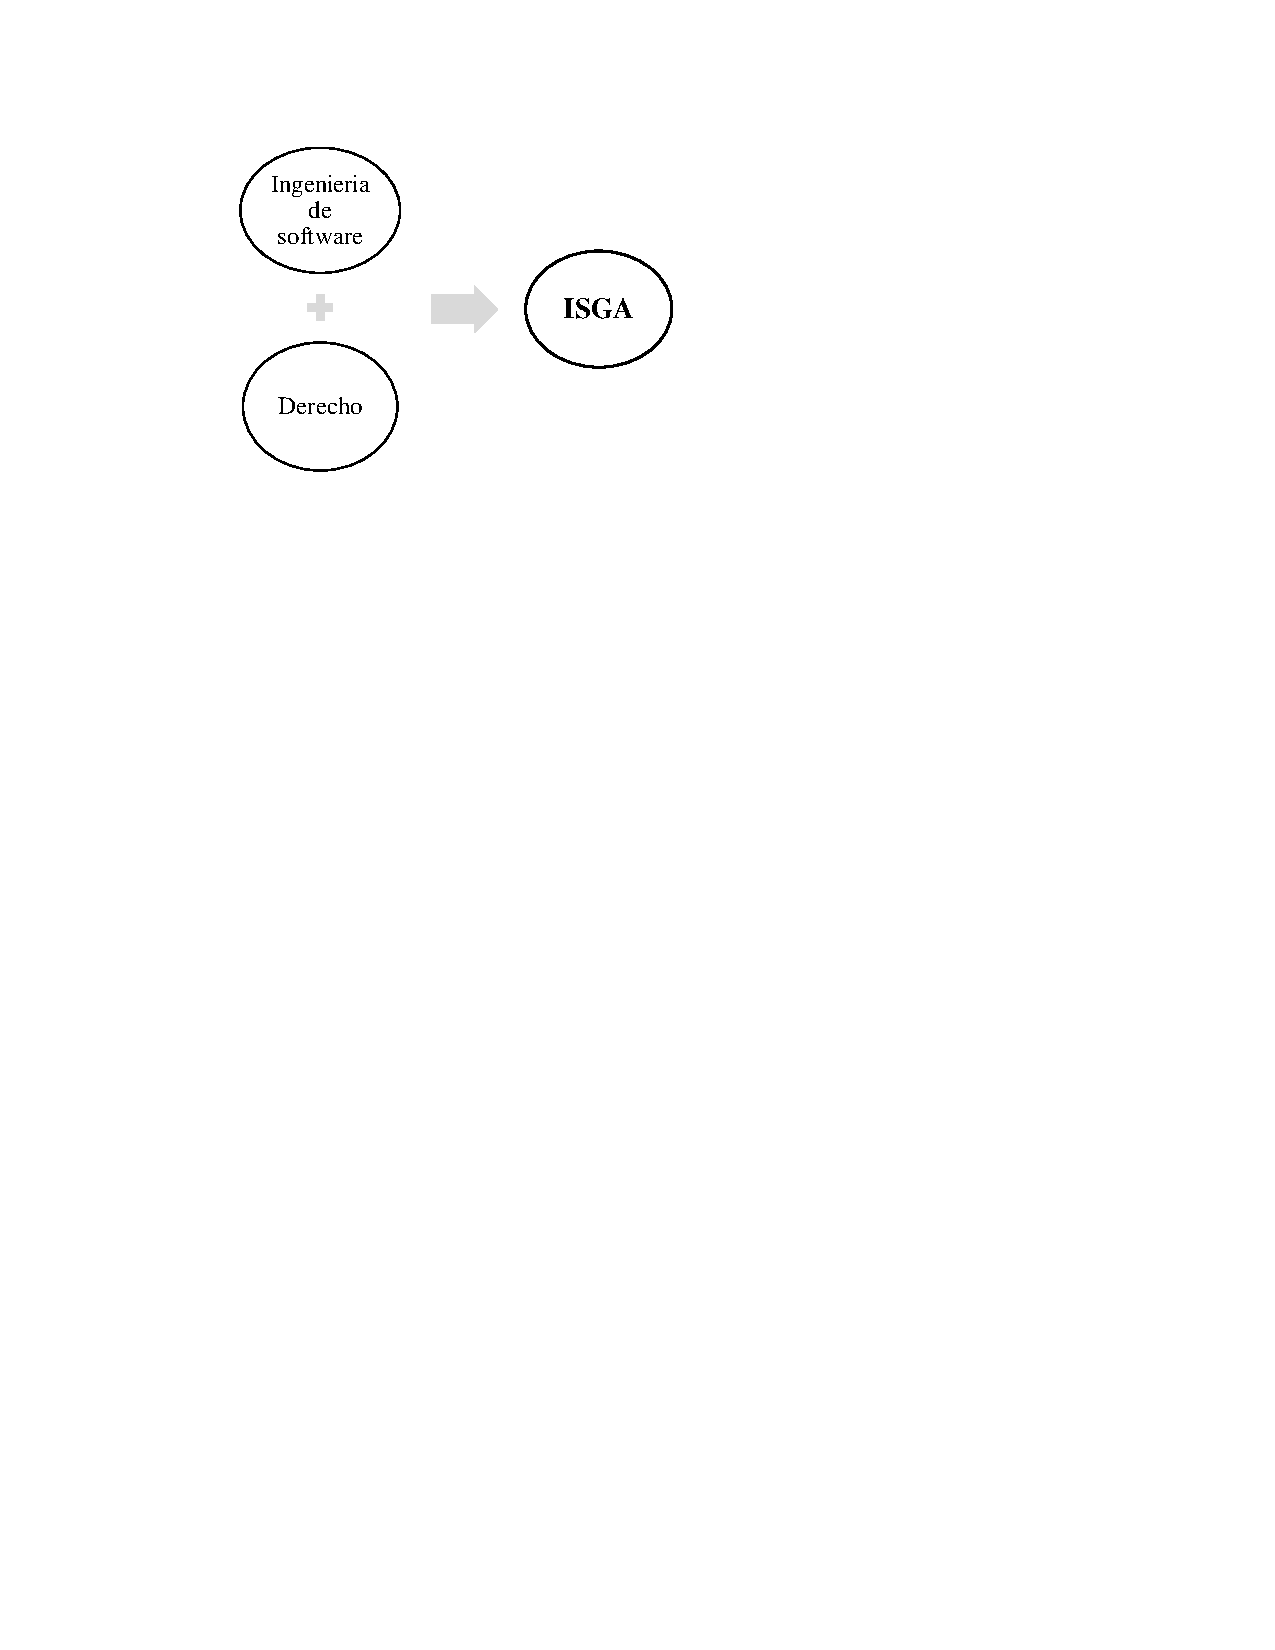
\includegraphics[width=0.85\columnwidth]{imagenes/pptesis.pdf}
\caption{Ingenieria de software para la gobernanza algorítmica}
\label{circulosfigdesd}
\end{figure} 

Grandes son los logros de la Ingeniería de Software y numerosos son los ingenieros que actualmente la dominan y son capaces de desarrollar sistemas complejos como Internet y otros que sobre ella funcionan (i.e. sistemas bancarios, redes sociales, aplicaciones como WhatsApp). Sin embargo, opinamos que el desarrollo de un \textbf{sistema} (conjunto de programas que se comunican entre ellos) para automatizar las leyes implica un grado de complejidad mayor porque sería un sistema para juzgar y controlar el comportamiento humano y, además, desafiaría el valor justicia. En ocasiones estos sistemas toman decisiones con grandes repercusiones como pagar o no pagar una multa, permitir o prohibir la entrada de una persona a un lugar, autorizar o no autorizar la aplicación de una vacuna o de una intervención quirúrgica, condenar o liberar a un acusado, etc. ¿Quién está capacitado para programarlos? Como explicaremos en la sección siguiente, pensamos que sería muy arriesgado encomendar esta tarea a los ingenieros de software actuales porque ellos están capacitados para programar sistemas rigurosamente específicos que arrojan respuestas lógicas precisas (falso o verdadero). Los sistemas legales no pertenecen a este grupo. Las leyes suelen ser ambiguas e incompletas, por ejemplo, suelen incluir palabras como “razonable” e “inmediatamente”, que no se pueden cuantificar ni codificar en lenguajes de programación .\footnote{Clack, C.D.: Smart contract templates: legal semantics and code validation. \url{http://www0.cs.ucl.ac.uk/staff/C.Clack/research/JDigitalBankingClack-AuthorPreprint.pdf} (2019), visited on 5 Dec 2020} Esto se debe al descuido de quienes las crean o porque es imposible elaborar leyes que anticipen todas las posibilidades o porque la ambigüedad da flexibilidad, algo muy útil para el juez que aplica la ley porque le da oportunidad de aplicar su criterio humano. Un problema adicional es que los ingenieros de software cometen errores. Además, documentado está que los algoritmos de IA no son infalibles; hay evidencias que demuestran que, en el ámbito penal, algoritmos usados para reconocimiento facial arrojaron decisiones sesgadas que favorecieron a unos grupos raciales y afectaron a otros. Este ejemplo muestra que el uso descuidado de la tecnología puede discriminar sistemáticamente a grupos minoritarios provocando una gran inequidad e injusticia. Los procedimientos judiciales solo pueden ofrecer una solución eficaz a los conflictos que se suscitan en la sociedad si son accesibles a los ciudadanos, empresas y cualquier persona que requiera justicia sin discriminación alguna. La discriminación racial debido al uso de leyes automáticas erróneamente programadas es solo uno de los riesgos, hay otros. Como solución a este problema, en este capìtulo sugerimos crear ISGA para formar ingenieros y abogados que sean capaces de entender los sistemas legales y evitar errores que pongan en riesgo los principios y derechos fundamentales del hombre. Definimos \textbf{ISGA} (Ingeniería de Software para Gobernanza Algorítmica) como una rama de la Ingeniería de Software tradicional que estudia la forma de transformar leyes escritas en lenguaje natural a programas de computadoras que ejecuten las leyes automáticamente.

Como veremos en la próxima sección, y como lo muestra la figura \ref{circulosfigdesd} ISGA precisa tanto de ingenieros en software con conocimientos en leyes como de abogados con conocimientos en programación.

\section{Principales problemas }

Nuestra visión de la GA plantea muchas cuestiones a resolver. Algunas de las más importantes son: (i) determinar a quien se le atribuirá la responsabilidad de que el código de la computadora sea fiel a la disposición legal y (ii) en qué medida las disposiciones legales pueden ser automatizadas. 

\subsection{¿Quiénes pueden automatizar las leyes? }

La GA tiene como objetivo automatizar las disposiciones legales. De esto se deriva la necesidad de contar con un enfoque interdisciplinario que reúna principalmente a informáticos y abogados. En esta sección analizaremos la intervención de los profesionales del Derecho y de la Tecnología para delimitar sus funciones y responsabilidades. 

Podemos distinguir dos fases en el proceso de automatización legal. De estas fases surge el grado de responsabilidad de los sujetos intervinientes:

\begin{itemize}

    \item{Programación y verificación} 
    \item{Validación e implementación}
    
\end{itemize}

\textbf{Programación y verificación de las leyes automáticas}

En la \textit{primera fase} que denominamos de “programación y verificación de las leyes automáticas”, los profesionales de la tecnología deben desarrollar los programas, traducir las disposiciones escritas a código de computadora y verificar que dichos programas cumplan con los requisitos y especificaciones del propósito previsto. Esta fase requiere conocimientos sólidos de programación. Consideramos que un especialista en tecnología (por ejemplo, un ingeniero de software) que esté debidamente capacitado en ISGA es competente para esta función. También, es importante destacar que en él recaerá la responsabilidad por los inconvenientes que puedan suscitarse en esta etapa.

\textbf{Validación e implementación de las leyes automáticas}

En la \textit{segunda fase}, se produce la “validación e implementación de la GA”. Una vez traducidas las disposiciones a código de computadora (leyes automatizadas) y verificadas por los tecnólogos es necesario que quienes la ejecuten tengan conocimientos suficientes de informática para poder utilizar los programas de GA. Los responsables de aplicar la ley (por ejemplo, jueces) son los que deben incorporar ese nuevo saber. Ellos deben capacitarse de forma consistente en tecnología. Por ejemplo, para ser designado juez se debería exigir conocimiento y experiencia de programación, lógica y algoritmo.

La segunda fase es de suma importancia debido a que se debe validar el código para garantizar que éste sea fiel a la disposición legal e implementar las leyes automáticas. Esto incluye aspectos clave para la asunción de responsabilidades por los problemas que puedan surgir. Por ejemplo, si se aplica una ley automática que no es fiel a la disposición escrita en lenguaje natural o si la ley automática no se aplica por desconocer su funcionamiento. 

Por lo tanto, el proceso de implementación de la GA requiere de abogados (pero también pueden intervenir especialistas de otras disciplinas como economistas, etc.) instruidos en ISGA. 

Como analizamos en otros capítulos de esta tesis, el cambio hacia equipos interdisciplinarios hace que cualquier aspecto del desarrollo de las leyes automáticas (smart contracts, blockchain) sea importante para cerrar la brecha entre la GA y la gobernanza tradicional. Creemos que los abogados y los ingenieros en software deben adquirir los conocimientos y herramientas de ISGA para desarrollar al máximo sus habilidades y destrezas en el desempeño de su labor. En última instancia, ellos tienen la la responsabilidad de proteger el valor justicia y el respeto a los derechos de las personas.  

\subsection{Efecto legal de la aplicación de las leyes automáticas}

Es importante que los abogados puedan validar que el efecto legal de cualquier disposición codificada o automatizada sea cierto, y que el efecto legal del código se alinee con el efecto legal previsto en la disposición legal. En este sentido, se debe distinguir los actos que ya se encuentren regulados y lo único que cambia es la transformación de la disposición a código de computadora; de aquellos otros actos que son novedosos para el derecho, por ejemplo, la transferencia de propiedad de activos en una blockchain o la propiedad de criptoactivos o NFTs. 

Además, hay varios aspectos a tener en cuenta en el proceso de validación. En primer lugar, antes de escribir el código, los profesionales del Derecho deben comprobar que la disposición sea legal. Luego, es esencial determinar que las disposiciones expresadas mediante una representación en código tengan fuerza legal. En la automatización de disposiciones legales mediante el código de computadora, los tribunales deben aceptar su aplicación para que produzca efectos legales. 

\subsection{La atribución de responsabilidad en la GA}

Merece la pena volver a subrayar que concebimos a las leyes automáticas como un sistema compuesto por varias (decenas) de herramientas interconectadas. Una de las herramientas más conocidas actualmente, y probablemente la que más controversias ha generado es la Inteligencia Artificial (IA) pero hay otras, como los contratos inteligentes (smart contracts) y las cadenas de bloques (blockchains). Todas estas herramientas se componen de programas, y por lo tanto, requieren de programadores y de leyes que las regulen. De ahí la necesidad de contar con profesionales que tengan conocimientos en Derecho y Tecnología.

La complejidad y particularidades de la convergencia entre el Derecho y la Tecnología derivan en la necesidad de colaboración entre científicos de distintas disciplinas que deben “hablar un mismo lenguaje”. Esto significa que, tanto los abogados como los tecnólogos, deben compartir habilidades y competencias. 

De todo lo que analizamos anteriormente, podemos concluir que, en la primera fase (programación y verificación), la atribución de responsabilidad recae sobre los profesionales de Tecnología, salvo que ellos prueben que la disposición escrita no era legal o carecía de validez.  En cambio, en la segunda fase (validación e implementación), la responsabilidad se traslada (salvo excepciones) a quienes deben aplicar las leyes automatizadas o GA y no pueden alegar desconocer su funcionamiento (jueces, abogados, etc.). 

Al comienzo de esta sección, nos preguntamos hasta qué punto las disposiciones legales pueden ser automatizadas. Entendemos que no todas las disposiciones pueden ser automatizadas en su totalidad. Muchas veces resulta esencial la intervención humana en determinadas etapas del proceso de automatización. Esta intervención puede deberse a diferentes motivos, tales como:

\begin{enumerate}
    \item Permitir las instrucciones externas, como pausar o detener el programa (por ejemplo, cuando una acción que sería tomada por el código se ha vuelto ilegal o porque la ley está desactualizada o derogada);
    
    \item{recibir datos externos donde no hay una fuente digital adecuada para la información requerida (por ejemplo, porque existe una laguna legal; y}
    
    \item{Pausar sus propias acciones para solicitar la toma de decisión/autorización a quienes tienen el deber de implementar la ley automática (por ejemplo, cuando se requiere una evaluación subjetiva).}
\end{enumerate}

El desarrollo del código del programa (especialmente para implementarlo en una blockchain) es una función especializada, que requiere profesionales experimentados en tecnología y equipos científicos. A la luz de esta naturaleza especializada (y compleja), y para asegurar que el código sea fiel a la disposición o acuerdo legal, es esencial el esfuerzo cooperativo involucrando (al menos) la capacidad y la experiencia de los profesionales de la Tecnología y del Derecho. Ambos deben abordar el contexto jurídico de las operaciones que están siendo automatizados para asegurarse de que el código sea compatible y coherente con las disposiciones que se deben automatizar. Por ello, es necesario la creación de una Ingeniería de Software para la Gobernanza Algorítmica que sea capaz de brindar competencias suficientes a aquellos que deben aplicar la GA.

\section{¿Qué se puede automatizar?}

\subsection{La automatización del contenido de la disposición legal}

La gobernanza algorítmica tiene como objetivo automatizar las disposiciones o reglas y un aspecto importante es automatizar su desempeño capturando la lógica de la normativa. 

Según algunos estudios realizados, existen dos modelos diferentes de automatización: a) aquel que separa lógicamente el código de la computadora de la ley automatizada. En este modelo, el código no es parte de la disposición legal y es simplemente una forma o herramienta en que la autoridad aplica la ley. Por lo tanto, el código no tiene ningún efecto legal. b) El otro modelo prevé que el código de computadora es parte de la ley y tendría efectos jurídicos. El código informático agregaría el aspecto novedoso de la operación autónoma, donde el código toma control sobre las actividades realizadas, toma decisiones basadas en eventos observados, y tiene mucha menos necesidad de intervención humana. Para asegurar la exactitud y confiabilidad de la ley automatizada, es esencial que la versión final del código se comporte de una manera fiel a la disposición legal. Como señalamos anteriormente, no es una tarea sencilla, la semántica en el Derecho y la Tecnología puede ser compleja. Ambas disciplinas tienen definiciones conflictivas de términos aparentemente inocuos, Una implementación técnica puede no ser legalmente efectiva o puede causar problemas legales inesperados o indeseables.

Por este motivo, el trabajo conjunto de abogados y tecnólogos es de suma importancia, y motiva fuertemente la discusión que incluye aquellos aspectos que deben ser considerados tanto por los profesionales de la tecnología que desarrollarán y verificarán como por los abogados que validarán para garantizar que el código sea fiel a la disposición y luego la implementarán. 

\subsection{Precisión de redacción}

No hay unanimidad de criterios en cuanto a la diferencia en la precisión de redacción entre el lenguaje humano usado por los abogados y el lenguaje formal de programación utilizados para crear código de computadora. Muchas veces, el humano tiene más flexibilidad para encontrar el método correcto a seguir para entender la redacción legal, que una máquina comprender el derecho para aplicarlo en lenguajes de programación. Es normal interpretar que las computadoras y la programación de computadoras son necesariamente deterministas, o son incapaces de manejar la ambigüedad. Sin embargo, hay quienes sostienen que esto no es verdad. El hardware de las computadoras modernas ha sido diseñado para ser determinista, y esa programación a menudo es determinista pero ello es así por conveniencia humana, porque a través de ese determinismo se logra el control sobre el hardware Aquellos que lo postulan afirman que es sencillo construir una computadora que no sea determinista, o crear un software que agregue un nivel de no determinismo y programar de una manera no determinista. Por lo tanto, las computadoras no necesitan ser deterministas y no necesitan estar restringidas a la simple lógica, pero ¿hasta qué punto es  necesario o deseable para automatizar la ley? Otra pregunta es: ¿cuánto del texto debe ser absolutamente claro y sin ambigüedades de antemano y cuánto se puede dejar para una interpretación posterior? Si tomamos el ejemplo de los contratos vemos que es interesante observar que los contratos tienen una mezcla de esos aspectos que deben ser muy detallada y cuidadosamente tenida en cuenta de antemano, sin ambigüedad, y aquellos aspectos que se expresan con cierto grado de ambigüedad ya sea porque (i) es poco probable que ocurran, y no valen el costo requerido para expresarlos con precisión, o (ii) las partes no pueden acordar términos precisos, y aceptan términos ambiguos. Además, la discreción puede ser un aspecto clave para responder a acciones potenciales de incumplimiento. 

La disposición legal o regla automatizada debe reflejar de manera fidedigna el contenido del texto legal. Existen casos en que la norma da lugar a interpretación subjetiva y es allí donde el programa no deberá ser determinista.

\section{Desafíos y funciones de lSGA para la Ingeniería de Software y para el Derecho }

La automatización de las leyes es un desarrollo innovador y disruptivo que trae consigo la necesidad de contar con profesionales que posean conocimientos multidisciplinarios de Derecho y de Programación. No está totalmente claro qué habilidades, derechos y responsabilidades deberían de tener los expertos en ISGA ni qué autoridad se las otorgaría. Algunos investigadores han analizado el problema y proponen que los ingenieros de software deben comprender bien las herramientas y técnicas especializadas en el desarrollo de aplicaciones descentralizadas, en particular aquellas que están orientadas a blockchain. Blockchain es la tecnología descentralizada que más controversias ha causado y que tiene más potencial para servir como base para automatizar las leyes. Por ejemplo, un grupo de expertos sugiere la creación de Blockchain-Oriented Software Engineering (BOSE) es decir software implementado para blockchain. Sin embargo, para la propuesta de esta tesis, el análisis de BOSE es incompleto porque omite evaluar las implicancias jurídicas. Además, se limita a estudiar únicamente los contratos y las blockchains. Nosotros pensamos que los contratos inteligentes y las blockchains son partes esenciales de la automatización de las leyes, pero no las únicas. Consecuentemente, recomendamos un enfoque más integral porque consideramos que los programas para automatizar leyes deben ser escritos bajo normas más estrictas que las de la Ingeniería de Software que conocemos. ISGA debe contemplar las siguientes funciones: 1) Educar profesionales que dominen la Ingeniería de Software y sean capaces de interpretar las leyes escritas en lenguaje natural de tal manera que sepan codificarlas correctamente en lenguajes de programación, a pesar de las ambigüedades de que las leyes adolecen. En otras palabras, necesitamos profesionales que dominen las tecnologías digitales y el Derecho. 2) Formar profesionales e instituciones que sean capaces de comprender, verificar, aprobar o rechazar un sistema (e.g., un programa escrito en Solidity) para automatizar leyes antes de llevarlo a la práctica. 3) Preparar profesionales (e.g., policías, jueces) que sean capaces de interpretar los resultados de un sistema para automatizar una ley, por ejemplo, un fallo judicial y las evidencias que el programa usó para arrojar el resultado; como aclaramos, algunas leyes por su complejidad (o para obtener eficiencia y flexibilidad) requieren de soporte humano. 4) Delimitar los roles e interdependencias de abogados e ingenieros de software incluyendo una especificación detallada de las facultades, obligaciones y responsabilidades de los profesionales de esta nueva disciplina. Sin embargo, resaltamos que los ingenieros de software no necesitan ser abogados ni los abogados ser ingenieros de software.\footnote{Borkert, K.: Lost in translation–legal challenges of smart contracts. \url{https://www.blockchain-hackathon.de/uncategorised/lost-in-translation-legal-challenges-of-smart-contracts/}}, 2018.
 Lo que sí se requiere es de un trabajo conjunto capaz de entender esta complejidad para no perderse entre las dos disciplinas. Como el uso de la tecnología en el sistema legal ya es irreversible, creemos que es el momento justo para unir los dos campos. Si no actuamos, en pocos años tendremos un gran problema difícil de controlar.

\section{Soluciones a los desafíos de ISGA }

La creación de ISGA nos enfrentará a dos problemas que merecen mucha atención. Primero, los conocimientos que los ingenieros de software y los abogados tienen actualmente de la automatización de las leyes son escasos. Segundo, los abogados se resisten a familiarizarse con la tecnología  . \footnote{ Hablamos de dominio pleno a nivel de algoritmos y programación que va más allá de conocer utilerías como Windows, Excell, Word, Power Point, navegadores, Google y whatsapp.} El problema se debe a que en la actualidad las carreras universitarias de Abogacía e Ingeniería de Software no tienen ninguna conexión entre sí. Por ende, la formación académica actual en las facultades de Derecho no es suficiente para enfrentar los desafíos planteados en una sociedad cada vez más digital. Pensamos que la solución más adecuada es que la carrera de abogacía enseñe conocimientos de lógica, algoritmos y programación que ayuden a los abogados a entender leyes automatizadas. Existen pocos programas de Derecho en todo el mundo que preparan a los estudiantes para las funciones legales emergentes. Hasta hace poco tiempo habían surgido grupos de estudios y carreras de postgrado en estos temas en las principales universidades del mundo como Stamford, Harvard, MIT y Viena. También en Argentina comienzan, aunque muy tímidamente, a ofrecerse algunos cursos y talleres de diversos temas jurídicos-tecnológicos. Sin embargo, aún no existe ninguno que tenga que ver con un cambio en la formación básica de la profesión de abogado. 

Según nuestro criterio, es necesario distinguir, por un lado, la formación en ISGA de los ingenieros de Software y por el otro, la de los abogados. Creemos que los primeros pueden adquirir algunos conocimientos legales, pero no creemos que puedan ser suficientes para implementar leyes automáticas con la responsabilidad que significa. El Derecho es una disciplina muy amplia y diversa. La aplicación de las normas conlleva asumir responsabilidades a la hora de su ejecución. Es necesario conocimientos sólidos en materia legal para poder implementarlo. En cambio, para los profesionales del Derecho, la situación es diferente. Opinamos que, un cambio en la estructura académica de formación jurídica con la incorporación de programación desde el inicio de la enseñanza universitaria puede formar abogados para ISGA. No obstante, reconocemos que es complicado concientizar a los abogados para que entiendan los beneficios de su estudio en el aprendizaje académico. Además, se trata de incorporar a una formación en ciencias sociales como es la carrera de Abogacía, el estudio de disciplinas provenientes de las ciencias exactas, como son la lógica, programación, etc.
En este capítulo explicamos la necesidad de crear una rama de la Ingeniería de Software para la Gobernanza Algorítmica (ISGA) y describimos las principales características, funciones y roles que deben cumplir los profesionales encargados de desarrollarla y aplicarla. Destacamos que la convergencia del Derecho y la tecnología debe responder a muchos desafíos y definir sus propias directrices para permitir su desarrollo e implementación. Uno de los mayores inconvenientes es el desconocimiento y confusión de abogados e ingenieros sobre el tema. Al sugerir la creación de ISGA, expresamos la importancia de investigar y desarrollar más la Ingeniería de Software orientada a la Gobernanza Algorítmica. Es muy probable que dentro de unos 15 años las leyes que ahora conocemos se apliquen automáticamente. Mucha y variada literatura internacional se ha publicado sobre IA \footnote{Corvalan, J.G.: Prometea, inteligencia artificial para transformar organizaciones públicas. \url{https://ialab.com.ar/libros/} (2019)} , blockchain y otras innovaciones digitales pero son escasas las que se refieren concretamente a las implicancias jurídicas que inevitablemente estas tecnologías ya están ocasionando y que los tribunales de justicia deberán resolver. Para lograr estos objetivos, creemos que los esfuerzos de cooperación entre las facultades de Derecho y de Ingeniería de Software serán esenciales para preparar a los estudiantes. Además, es útil pensar cómo deberán estructurarse sus relaciones y cómo deberán cumplir con los deberes impuestos a cada una de ellas. Estas instituciones deben centrarse en el aprendizaje permanente y capacitación adecuada de tecnología para abogados e ingenieros de software y definir sus respectivas funciones (derechos, obligaciones y responsabilidades). Las instituciones deben reconocer que es su responsabilidad colectiva capacitar y asesorar a quienes serán responsables de automatizar las leyes. Una pregunta más intrigante es si el uso de la tecnología, puede ayudar no solo a automatizar y hacer más eficientes los sistemas jurídicos que nos gobiernan actualmente, sino también a cambiarlos radicalmente y liberarlos de las deficiencias que los aquejan. Quizá la tecnología ayude a evitar las tiranías y a erradicar algunos de los males arraigados que afectan a los sistemas democráticos actuales como la “tiranía de las mayorías” y “el todo o nada” que discrimina a las minorías derrotadas en las votaciones . Pensamos que bien programadas y usadas por expertos en ISGA, las leyes automáticas pueden ayudar a crear democracias más incluyentes y transparentes que tomen en cuenta conceptos fundamentales como los derechos humanos, la ética digital, justicia digital, el derecho a la privacidad y el derecho al olvido. La tecnología abre muchas puertas para innovar el sistema jurídico. Sin embargo, la automatización descuidada podría llevar a leyes inflexibles y deshumanizadas impulsadas por programas erróneos que ignoran las particularidades de los individuos y de las minorías [19]. Coincidimos con Gasset et. al. [9] que sugieren que el trabajo de las universidades es clave para permitir y facilitar un grado mayor de interoperabilidad entre las ciencias técnicas y sociales. La combinación de varios enfoques interdisciplinarios es un aspecto importante que aún no ha sido tomado en cuenta por la comunidad técnica y jurídica. Opinamos que un trabajo conjunto conducirá a nuevas y mejores estrategias para enfrentar los desafíos que plantea la automatización de las leyes. Por ejemplo, los investigadores necesitan indagar si ISGA se puede adaptar a diferentes metodologías de la ingeniería de software y de la ciencia jurídica. Se debe examinar si los programas y sistemas desarrollados bajo los principios de ISGA se pueden integrar con los programas desarrollados en el pasado, con Ingeniería de Software tradicional. Uno de los cuatro objetivos de la brújula digital 2030  que explica los planes digitales de la Unión Europea para los próximos años contempla una población con profesionales digitales altamente capacitados. Nos atrevemos a decir que la creación y aplicación de ISGA requiere de un esfuerzo multidisciplinario que involucra a expertos en Tecnología, Ciencias de la Computación, Derecho, Derechos humanos, y otros.





\chapter{GOBERNANZA ALGORÌTMICA}
\label{goberalgoritmica}
En este capítulo, comenzamos con una introducción a las leyes automáticas; y explicamos lo que entendemos por gobernanza algorítmica en el contexto de esta tesis. Luego delineamos las características principales de la gobernanza algorítmica y analizamos los elementos que la componen y que no pueden faltar, así como otros elementos especiales que pueden ayudar a su funcionamiento. También identificamos y proporcionamos ejemplos de gobernanza algorítmica para explicar la diferencia con la gobernanza tradicional. Posteriormente, dedicamos una sección para resumir las distintas etapas de su formación y señalamos algunas implicancias jurídicas. Planteamos los principales riesgos y desafíos asociados con la utilización, Por último, señalamos lo que se necesita en el ámbito legal para cerrar la brecha con la gobernanza tradicional. 
A lo largo del capítulo, aclaramos cuestiones terminológicas referidas, en su mayoría, a conceptos técnicos, así como también a otros conceptos que puedan dar lugar a interpretaciones erróneas sino se explican suficientemente.

\section{Nociones generales}

La gobernanza algorítmica (GA) es un término novedoso para el Derecho y poco comprendido por abogados y otros profesionales de las ciencias sociales con escasos conocimientos de tecnología. Se compone de varios conceptos técnicos (smart contracts, blockchain, etc.) que se examinarán particularmente en los capítulos siguientes. En este capítulo, se expondrán las definiciones más importantes para que este trabajo sea accesible a personas del campo de la técnica y de otras ciencias.

En un sistema jurídico, la GA comprende la codificación en código informático de la mayoría de las normas o reglas que imperan en un país y que se ejecutan de manera automática. Por ejemplo, en el sistema tributario, para obtener el monto del impuesto al valor agregado (IVA) que anteriormente solía estar escrito en papel y se aplicaba manualmente al revisar las facturas, ahora ha sido codificado en uno (varios) programas que se han instalado en las maquinas de pagos de los comercios para que cobren el 15 \% a cada comprador y luego envíen (ley codificada) ese dinero directamente a las arcas del Estado. Otro ejemplo práctico, es la ley de pensiones (jubilación). Al ser traducida de papel a un programa de computadora por un ingeniero de software e instalado el programa en los sistemas de nomina de las empresas, cuando un trabajador se jubila, esa ley automatizada autoriza directamente el cobro de la jubilación a ese trabajador.

El fenómeno de la gobernanza algorítmica es parte de una tendencia histórica hacia la mecanización. Sociólogos desde los tiempos de Weber han destacado las formas en que la organización jurídico-burocrática del Estado está sujeta a las mismas tendencias modernizadoras que el diseño de las fábricas (Kanter, 1991; Weber, 1947). Desde los albores de la era de la computadora se han hecho intentos para automatizar parte o todo el proceso. Sin embargo, los sistemas que se utilizan hoy en día son diferentes a los de sus antepasados históricos. Las tecnologías que facilitan la automatización de la gobernanza sin duda se construyen sobre estructuras preexistentes, beneficiándose de las innovaciones mecánicas anteriores. Pero la velocidad, escala y ubicuidad de las tecnologías actuales superan lo que eran en el pasado. Además, los avances en las herramientas digitales como el aprendizaje automático y la recopilación de datos, entre muchas otras, permiten una automatización que antes no hubieran sido posibles. \footnote{Danaher, John Hogan, Michael J, Noone1, Chris, Kennedy, Ronan, Behan, Anthony, De Paor, Aislin,
Felzmann, Heike, Haklay , Muki, Khoo, Su-Ming, Morison, John, Murphy, Maria Helen, O’Brolchain, Niall, Schafer, Burkhard. Shankar, Kalpana, “Algorithmic governance: Developing a research agenda through the power of collective intelligence”, Big Data and Society, 2017
}

La automatización producida por la convergencia entre el Derecho y la Tecnología sucede a finales del siglo XX y su desarrollo ocurre paulatinamente en el tiempo, alcanzando diferentes niveles (ver capítulo \ref{Introducción}, sección XX). Los avances van desde la digitalización y almacenamiento de la información en grandes bases de datos virtuales hasta la automatización de la toma de decisiones. Esta última significa transformar las disposiciones legales en código informático (ley automática). Ya se están dando los primeros pasos en distintos ámbitos de la sociedad; no obstante ser un enorme desafío por muchas razones, como, por ejemplo, la ambigüedad del lenguaje humano y la necesidad de que algunas normas legales sean flexibles y dependan de los hechos, Muchos son los ejemplos donde el derecho y la tecnología se unen: en el derecho a la salud: historias clínicas digitarles, recetas digitales, etc., en el derecho tributario y financiero: regulaciones fiscales y financieras para la toma de decisiones automatizada, por ejemplo, herramientas específicas para impuestos, contabilidad y crédito; en el derecho civil y comercial: contratos digitales, firmas digitales, etc. 

Los primeros elementos de automatización que han estado en uso durante muchos años son poco probable que den lugar a nuevos problemas legales. Por ejemplo, el pago mediante débito bancario. En cambio, las innovaciones recientes que involucran automatizaciones más sofisticadas y que tienen que ver con la toma de decisiones (gobernanza algorítmica) no son familiares para el Derecho y, por lo tanto, es presumible que den lugar a nuevos planteos legales. Por ejemplo, en un proceso judicial, la sentencia judicial automatizada donde se sustituye al juez en su veredicto, o en el ámbito contractual, un contrato redactado principal o únicamente en código y registrado en una blockchain. En las próximas secciones analizaremos varias de sus implicancias jurídicas más relevantes.

\section{Algunas aclaraciones terminológicas}

En la gobernanza algorítmica se usan algoritmos para gobernar, aunque hay autores que hablan del uso de programas ejecutados por computadoras para gobernar. En ciertos contextos, las palabras algoritmo y programa se pueden usar como sinónimos. Sin embargo, en otros es necesario no perder de vista que son conceptos distintos: un \textbf{algorítmo}, como se definió anteriormente, es la especificación de la solución de un problema escrito en papel, en lenguaje humano usando diagramas.\footnote{Dourish, P.: “Algorithms and their others: Algorithmic culture in context”. Big Data
\& Society 1(11), Jul–Dec 2016
}  Un \textbf{programa} es dicha especificación escrita en un lenguaje de programación (p.ej., Java, Python) y provista de datos de entrada que una computadora ejecuta para resolver un problema especificado. Por ejemplo, hay algoritmos que describen las operaciones para encontrar el mínimo común múltiplo de dos números enteros y estos algoritmos se pueden implementar en distintos lenguajes de programación con programas escritos en esos lenguajes. Por otro lado, un \textbf{código} es, en su forma más simple, un lenguaje utilizado para dar instrucciones a las computadoras. Por ejemplo, el sistema numérico de dos dígitos (binario), o bit: el "0" y el "1".

En la última década, la GA ha ganado una mayor atención política y jurídica cuando se intentan diseñar procesos sociales y económicos mediante el uso de sistemas algorítmicos. Hoy en día, los algoritmos son parte de la vida cotidiana, pero sus impactos apenas comienzan a ser discutidos. Desde las recomendaciones de motores de búsqueda personalizados para la programación de vuelos del aeropuerto, verificaciones de crédito y decisiones comerciales y financieras, los algoritmos se han vuelto virtualmente indispensables para el análisis y la toma de decisiones en nuestros entornos saturados de datos .\footnote{Gillespie T., “The Relevance of Algorithms”. In: Gillespie T, Boczkowski PJ, Foot KA (eds) Media Technologies: Essays on Communication, Materiality, and Society, pp. 167–193. The MIT Press, Cambridge, MA. 2014} Por esta razón, algunos autores sitúan a la GA en la intersección de la digitalización, la dataficación y la gobernanza a través de la tecnología. \footnote{Wilsdon J (ed) (2001) Digital Futures: Living in a Networked World. Routledge, London. Danaher J, Hogan MJ, Noone C et al. (2017) Algorithmic Governance: Developing a Research Agenda Through the Power of Collective Intelligence. Big Data \& Society 4(2), 2053951717726554.} Entendemos por \textbf{gobernanza} a la toma de decisión o aplicación de la ley, norma o regla. La literatura destaca cómo la digitalización crea activos de información más allá de la capacidad de procesamiento de la inteligencia humana (a menudo denominado \textbf{Big Data)}, al tiempo que ofrece la oportunidad de utilizar herramientas programadas por computadora (software) alimentado por un conjunto de reglas y comandos lógicos (algoritmos). En estos complejos sistemas computacionales, los algoritmos definen las formas en que el software moviliza los activos de información para alcanzar fines particulares .\footnote{Gillespie T, ib.}

Algunos gobiernos ya están incorporando poco a poco, y de manera aislada, algoritmos que ayudan a realizar sus tareas. Por ejemplo, en Hacienda, se los utiliza para calcular el cobro de impuestos. También, sistemas judiciales han experimentado con el uso de algoritmos en la investigación penal. Por ejemplo, han empleado muestras de ADN y datos de GPS para identificar y descartar a sospechosos de haber cometido un delito. \footnote{Palmiotto, F.: “The black box on trial: The impact of algorithmic opacity on fair
trial rights in criminal proceedings”. In: Ebers, M., Gamito, M.C. (eds.) Algorithmic
Governance and Governance of Algorithms. Springer, 2021}


\section{¿Qué es la gobernanza algorítmica?}
Varios son los términos que los estudiosos usan para referirse a la gobernanza algorítmica: lex cryptographia\footnote{\cite{PrimaveraAaron2018} }, leyes automáticas, leyes computables \footnote{Computational Law. 2021, \url{https://law.mit.edu}}, leyes programables, leyes algorítmicas y gobernanza digital, entre otros. Sin embargo, consideramos que el término más descriptivo y el más aceptado actualmente es gobernanza algorítmica (GA) y es el que utilizaremos en esta tesis.

En un sentido amplio, podemos definir a la \textbf{ gobernanza algorítmica } como un conjunto de reglas y procesos regidos por algoritmos que toman decisiones de manera automática. Por ejemplo, la aplicación automática de una pena ante la ocurrencia de un delito tipificado en el Código penal.

Una gobernanza algorítmica funcionando a plenitud es un sistema integrado pero descentralizado. En dicho sistema, los programas que actualmente usan aisladamente la gobernanza tradicional son codificados como contratos inteligentes. Estos contratos son instalados en plataformas descentralizadas como las cadenas de bloques (blockchains) y colaboran entre ellos para aplicar las leyes automáticamente. Predecimos que se usarán blockchains privadas administradas por el gobierno y blockchains públicas como, por ejemplo, Ethereum. La elección dependerá de varios factores, como la necesidad de identificar plenamente a cada individuo (ver capítulo~\ref{gatoigsa}).	

\section{La gobernanza algorítmica y la ley automática}

No debemos confundir el término gobernanza algorítmica como sinónimo de ley automática. En realidad, la gobernanza algorítmica presupone la existencia de una ley automática. 

Definimos a la \textbf{ley automática}, aunque quizás el término más apropiado sea “ley automatizada”, como un sistema algorítmico que, a través de un procedimiento transforma una ley, norma o regla escrita en lenguaje natural, en código de computadora. En resumen, es un sistema algorítmico que automatiza una ley, norma o regla. Mientras que la gobernanza algorítmica es la aplicación efectiva (toma de decisión) de esa la ley automática.

La figura ~\ref{figdecirculos} muestra la composición de la gobernanza algorítmica

\begin{figure}
\centering
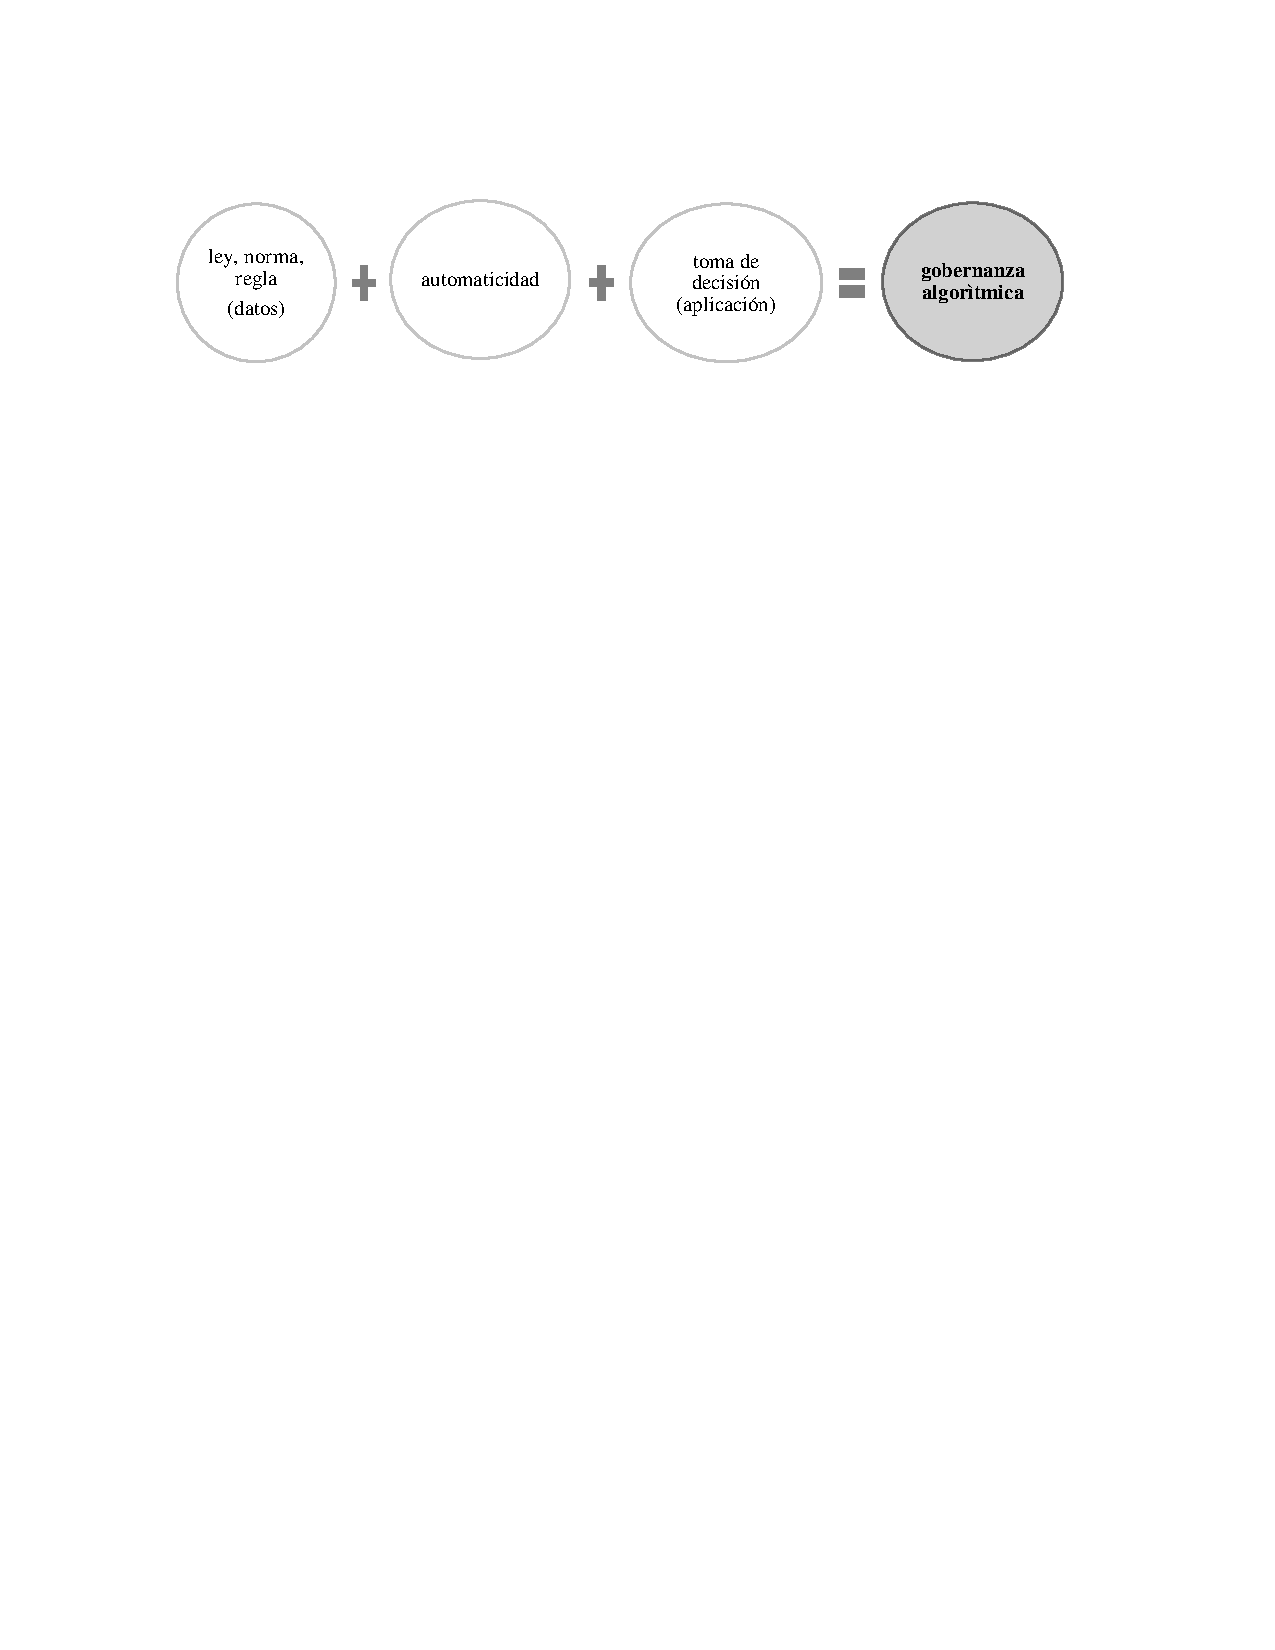
\includegraphics[width=0.85\columnwidth]{imagenes/figdecirculos.pdf}
\caption{Composición de la gobernanza algorítmcia.}
\label{figdecirculos}
\end{figure} 

\section{Principales características }


Las dos características principales de la gobernanza algorítmica son:

\begin{itemize}
    \item La automaticidad (leyes automáticas)
    
    \item La toma de decisión (aplicación de las leyes automáticas)
\end{itemize}

El objetivo de automatizar una norma es que se aplique sin necesidad de la intervención humana, salvo en casos excepcionales, cuando el intelecto humano sea indispensable. En realidad, el uso de programas informáticos para automatizar las leyes no es nuevo y, como expresamos anteriormente, su aplicación ocurre diariamente en los pagos bancarios automatizados, las compras en línea, entre muchos otros ejemplos. Sin embargo, a través de los años el grado y variedad de automatización ha crecido y evolucionado a un ritmo que ha dejado muy por detrás la regulación legal surgiendo verdaderos problemas jurídicos. En las próximas secciones analizaremos algunas de ellos.

\section{Elementos de las leyes automáticas}


Decimos que las leyes automáticas son un sistema porque se trata de un conjunto de elementos o componentes relacionados entre sí que funcionan como un todo. Es importante identificar cada uno de esos elementos para estudiarlos de manera independiente y simplificar el problema.

\textbf{Ley, norma o regla escrita en lenguaje natural (Datos):} cualquier disposición cuya finalidad sea regular el comportamiento de los individuos en sociedad y cuyo incumplimiento sea pasible de sanción. En sentido técnico esa disposición es un conjunto de datos. 

\textbf{Contrato inteligente \textit{(Smart contracts):}} entendido como el código de computadora que, ante la ocurrencia de una condición (o condiciones específicas), es capaz de funcionar automáticamente de acuerdo con funciones pre especificadas. Es la herramienta más importante, debido a las implicaciones jurídicas que involucra. Dedicamos el capítulo \ref{Contratos digitales} para explicarlo en detalle. 

\textbf{Descentralización:} Cuando hablamos de descentralización en el contexto computacional, nos referimos a que los servicios de aplicaciones se llevan a cabo mediante dispositivos informáticos individuales o nodos en una red distribuida, sin una ubicación central.  La web es la aplicación descentralizada más grande del mundo. Al ser la plataforma de aplicaciones más ubicua jamás desarrollada, la convierte en la base perfecta para la informática descentralizada. Un ejemplo de sistema descentralizado es una blockchain que consiste en un método de registro de datos de forma estructurada. Los datos generalmente se agrupan en "bloques" que están matemáticamente vinculados o "encadenados" al bloque anterior. En el capítulo \ref{Descentralización} describimos éste y otros sistemas descentralizados.

Este sistema automatizado, a su vez, puede estar compuesto por varias (decenas) de elementos o herramientas interconectadas. Una de las herramientas más conocidas actualmente y que más controversias ha generado es la Inteligencia Artificial (IA) pero hay otras, como Big Data, IoT, Machine Readable Legislation, etc. Explicamos brevemente algunas de las más importantes:

\textbf{Internet de las cosas, en inglés \textit{Internet of Thing}s (IoT)} involucra un ecosistema complejo y de gran escala de dispositivos y servicios, con la computación en la nube. La importancia de IoT para la GA es la de proporcionar datos de entrada a los programas que automatizan las leyes (Por ejemplo, mediante el uso de IoT se puede llegar a conocer donde se encontraba una persona sospechosa a la hora de cometer un homicidio. Otro ejemplo, es conocer la velocidad del auto a la hora en que se produjo el accidente. Los actuadores de IoT \textit{(actuators)}\footnote{Un actuador es un tipo de motor que se encarga de mover o controlar un mecanismo o sistema.}  pueden ayudar a aplicar la ley, por ejemplo, un actuador cierra la barrera para impedir que pasen los autos cuando va a pasar el tren, abre la puerta de la casa que se alquiló cuando se pagó el alquiler, etc.

\textbf{Inteligencia artificial:} es la habilidad de una máquina de presentar las mismas capacidades que los seres humanos, como el razonamiento, el aprendizaje, la creatividad y la capacidad de planear . \footnote{\url{https://www.europarl.europa.eu/news/es/headlines/society/20200827STO85804/que-es-la-inteligencia-artificial-y-como-se-usa}} Algunas tecnologías con inteligencia existen desde hace más de 50 años, pero los avances en la informática, la disponibilidad de enormes cantidades de datos y nuevos algoritmos han permitido que se den grandes avances en los últimos años. Algunos ejemplos son: los motores de búsqueda que aprenden de la gran cantidad de datos que proporcionan sus usuarios para ofrecer resultados de búsqueda relevantes; los asistentes personales digitales de los teléfonos móviles; el uso de los asistentes virtuales que responden a preguntan, dan recomendaciones y ayudan a organizar las rutinas de sus propietarios; las casas, ciudades e infraestructuras inteligentes: los termostatos inteligentes aprenden de nuestro comportamiento para ahorrar energía, mientras que los desarrolladores de ciudades inteligentes esperan poder regular el tráfico para mejorar la conectividad y reducir los embotellamientos; los vehículos de conducción autónoma. En el campo legal, se está utilizando la IA, por ejemplo, para crear versiones digitales de códigos legales (civil, comercial, penal, etc.) y para resolver problemas legales y hasta actuar como árbitros o jueces . El objetivo es utilizar sistemas sofisticados de inteligencia artificial con conocimiento del sistema legal para ayudar a elaborar y simplificar la nueva legislación .\footnote{\cite{Omohundro2014}, “Cryptocurrencies, Smart Contracts, and Artificial Intelligence”}

\textbf{Big Data o macrodatos: "inteligencia de datos"} hacen referencia a conjuntos de datos de tamaño tan grande y complejo y de tal variabilidad que precisan de herramientas tecnológicas, como la inteligencia artificial, para procesarlos. La Comisión Europea estima que el volumen global de datos incrementará en un 530\% para 2025 con respecto a 2018. Los seres humanos producen estos datos: en aplicaciones móviles, páginas web, redes sociales, transacciones comerciales, registros gubernamentales en línea. También los Iot producen millones de datos.

\textbf{Machine readable legislation (legislación legible por máquina)} significa codificar la información para que sea legible por la máquina. Los documentos legislativos son una clase importante de los documentos legales que regulan casi todas las áreas de la vida de las personas. La introducción de modernas tecnologías de la información en el dominio legal trae numerosos beneficios sobre todo por el caudal de información que los abogados deben conocer. Sin embargo, muchas veces los documentos legales no son fáciles de interpretar y se necesita de los profesionales del Derecho para comprenderlos.  En las últimas décadas, la informática se ha convertido en un instrumento para ofrecer una variedad de métodos aplicados en el dominio jurídico .\footnote{Cvejić, Andrija, Cvejić, Aleksandar, Grujić, Katarina-Glorija, Marković, Marko, 
“” Automatic Transformation of Plain-text Legislation into Machine-readable Format”, Conference Paper · March 2021 \url{https://www.researchgate.net/publication/349947228_Automatic_Transformation_of_Plain-text_Legislation_into_Machine-readable_Format?enrichId=rgreq-7ff40d5be0097488f37eca39fe063316-XXX&enrichSource=Y292ZXJQYWdlOzM0OTk0NzIyODtBUzoxMDc4NDkxMDEzNDg0NTQ0QDE2MzQxNDM3MDM1ODQ\%3D&el=1_x_2&_esc=publicationCoverPdf}
}


\subsection{Procedimiento de formación de la GA}

Para que la gobernanza algorítmica funcione debe seguirse un procedimiento determinado. De manera resumida podemos dividirlo en tres etapas:




\begin{figure}
\centering
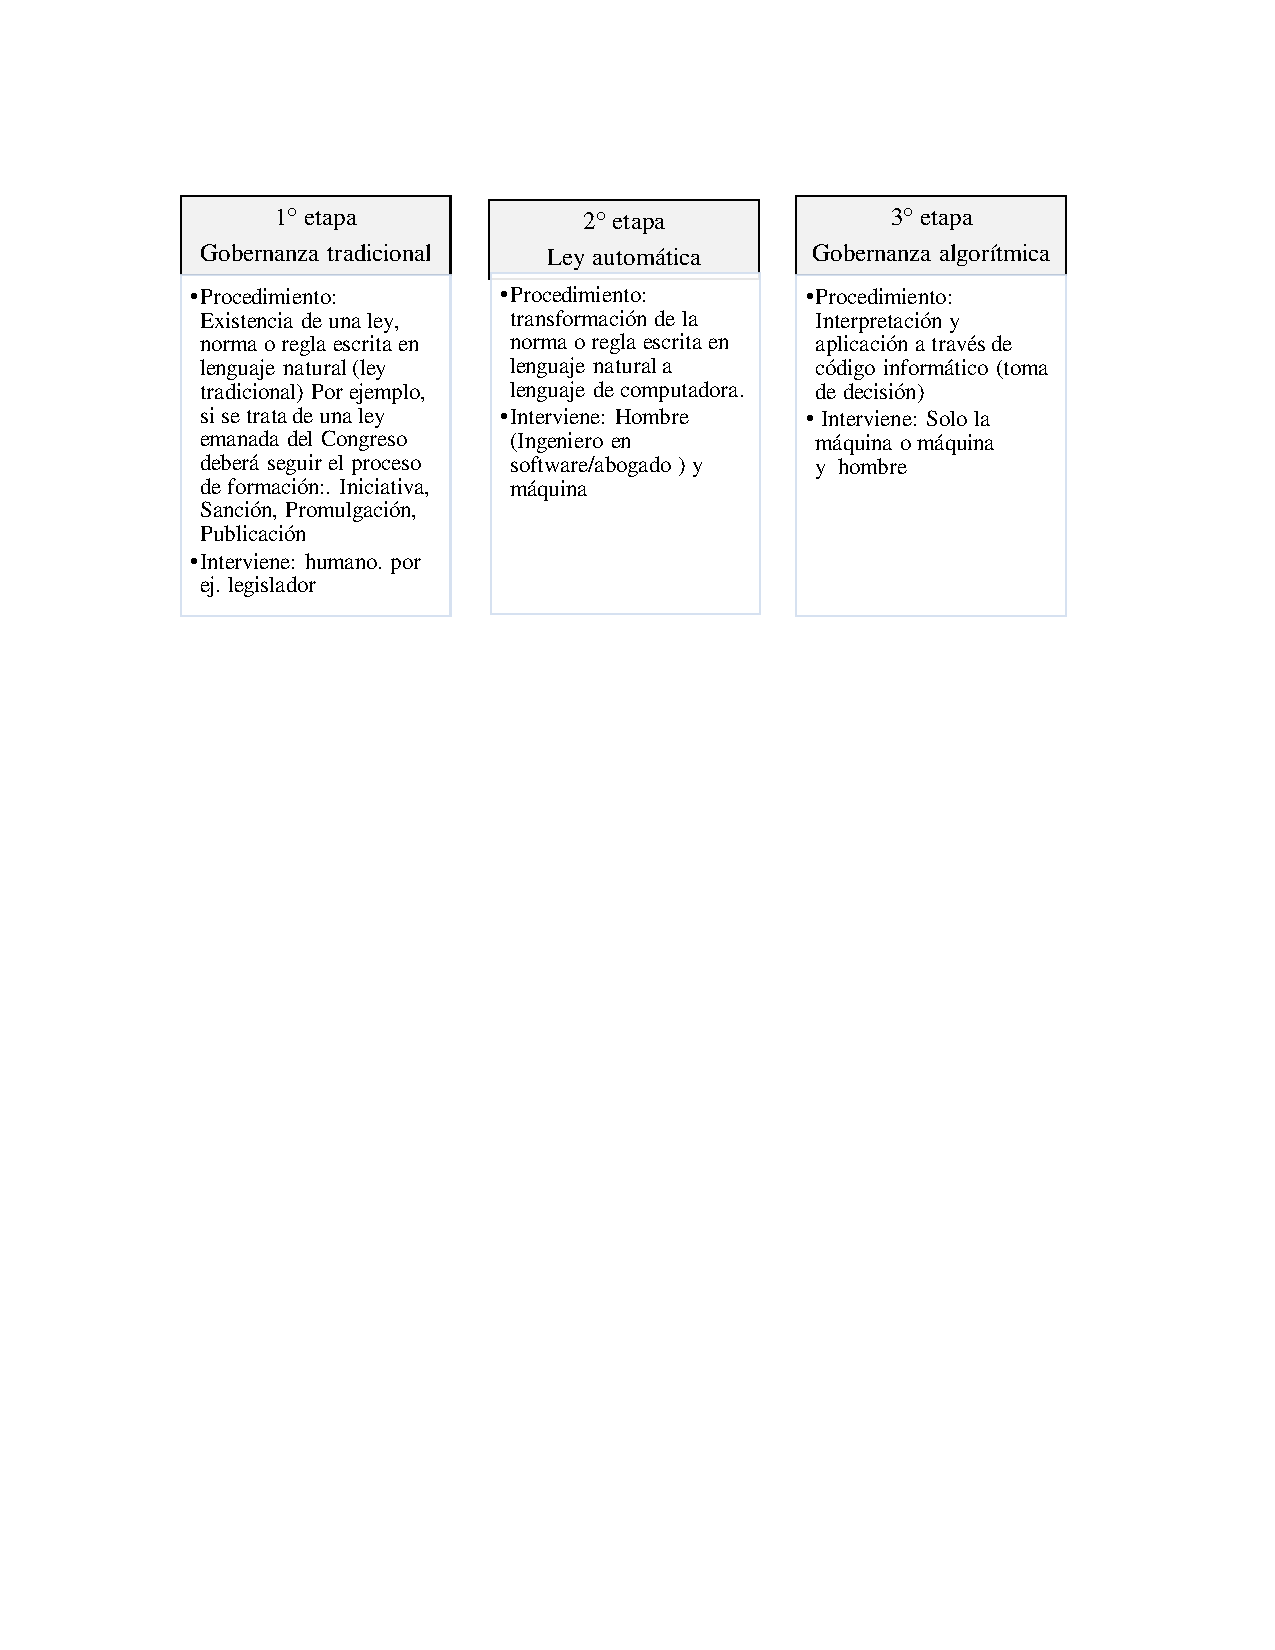
\includegraphics[width=0.85\columnwidth]{imagenes/tabladega.pdf}
\caption{Etapas en el procedimieento de la Gobernanza Algorítmica.}
\label{tabladega.pdf}
\end{figure} 

La \textit{primera etapa} de "formación de la gobernanza algorítmica" tiene que ver con la existencia de una disposición emanada de un humano. Por ejemplo, una ley que proviene del órgano legislativo de gobierno o un decreto del Poder Ejecutivo. La creación de una norma siempre es decisión del hombre que ve la necesidad de regular una determinada conducta. En esta primera etapa, la gobernanza tradicional y la algorítmica coinciden. En la \textit{segunda etapa}, se traducen las normas escritas en lenguaje natural (gobernanza tradicional) a código de computadora, es decir a un lenguaje de máquina. Esta fase es lo que denominamos leyes automáticas y que muchas veces algunos autores confunden con la siguiente etapa de aplicación o toma de decisiones. La redacción codificada de la norma debe realizarlo una persona con conocimientos en computación. Finalmente, la \textit{tercera etapa}, consiste en la toma de decisiones o la aplicación de las leyes automatizadas. En la GA esta etapa es realizada por la máquina. No obstante, en determinadas situaciones puede solicitar la intervención de un humano.

\subsection{Responsabilidad del codificador}

La atribución de responsabilidad en la GA es un tema esencial que aún hoy en día no está resuelto. Si nos basamos en las tres etapas de formación de la GA (ver sección anterior) observamos que, en la primera fase, la asignación de responsabilidad es la misma que para la gobernanza tradicional. La segunda y tercera etapa, es decir la relacionada con la ley automatizada y su aplicación, plantean cuestiones jurídicas innovadoras que es preciso estudiar en profundidad. Ver capítulo XX

\subsection{¿Quién controla?}

La creación de un organismo de supervisión gubernamental que se encargue de la regulación de algoritmos es una posibilidad para el futuro. Este organismo deberá centrarse en requisitos tales como el nivel de transparencia o calidad en términos de errores, riesgos  de muerte, o lesiones causadas por algoritmos o software, junto con las conductas que atentan la seguridad y otras preocupaciones.  \footnote{\cite{Almeida2016}, “What is Algorithm Governance?"}

\subsection{ Diferencia entre la gobernanza algorítmica y la gobernanza tradicional}

La gobernanza algorítmica se diferencia de la \textbf{gobernanza tradicional}  porque en esta última, los humanos (ej. jueces, abogados, auditores, etc.) son protagonistas y se encargan de tomar todas las decisiones, casi siempre apoyados, de alguna manera, por tecnología. En la gobernanza algorítmica, en cambio, las decisiones son tomadas automáticamente por programas y los humanos intervienen únicamente cuando los programas que automatizan las leyes son incapaces de tomar las decisiones de forma certera. Estos programas han sido estudiados desde hace décadas, en 1997 Szabo  los llamó contratos inteligentes (\textit{smart contracts}- en inglés). Nos referiremos a ellos en el capítulo \ref{Contratos digitales}.


\begin{table}
\centering
\begin{tabular}{|c|c|c|} 
 \hline
Propiedad & Gobernanza tradicional & Gobernanza algorítmica \\
\hline
 Imparcialidad            & No  & Si \\ 
Flexibilidad             & Si  & No \\ 
Regulación legal         & Si  & No \\ 
Mayor grado de justicia  & No  & Si \\
Alto grado de eficiencia & No  & Si \\
Alto costo de tecnología & No  & Si \\ 
Menos gastos judiciales  & No  & Si \\ 
Mayor transparencia      & No  & Si \\ 
\hline
\end{tabular}
\caption{Diferencias entre la gobernanza tradicional y la gobernanza algorítmica.}
\label{tab:gobtrad_vs_gobalgo}
\end{table}


La Tabla \ref{tab:gobtrad_vs_gobalgo} tiene por finalidad arrojar un poco de luz sobre este tema resumiendo las principales diferencias entre la gobernanza tradicional y la gobernanza algorítmica. Argumentamos que un programa de computadora es más confiable y transparente y, por ende, más justo, que un abogado, médico, contador a los que le cuestionamos, por ejemplo, el estricto cumplimiento del secreto profesional (ver Cap. X). En la mayoría de las veces, la gobernanza algorítmica puede actuar con mayor eficiencia y de una manera más inclusiva. Especialmente consideramos que los riesgos que produciría la aplicación de leyes automáticas no son tan altos como algunos autores sostienen. Además, los gastos propios del proceso judicial se reducirían considerablemente al no ser necesario atravesar las instancias judiciales. El principal inconveniente es la falta de conocimiento por parte de la comunidad para aprovechar eficazmente estas herramientas. Esta ignorancia también se produce en el ámbito público donde la ausencia de interés se traduce en la escasa inversión en tecnología.

Si bien la gobernanza algorítmica tiene numerosos beneficios, es cierto que aún faltan resolver varias cuestiones jurídicas como, por ejemplo, su regulación legal o la atribución de responsabilidad ante la falla del sistema. 

A diferencia de la gobernanza tradicional donde la regulación es interpretada y aplicada en su totalidad por un humano (por ej. un juez), en la gobernanza algorítmica siempre interviene una computadora en la toma de decisiones. Esta decisión puede ser total o parcialmente emitida por la máquina. La participación humana en la gobernanza algorítmica se debe a la complejidad de las leyes. Estas suelen ser ambiguas e incompletas, por ejemplo, suelen incluir palabras como “razonable”, e “inmediatamente”, que no se pueden cuantificar ni codificar en lenguajes de programación . \footnote{\cite{Christopher2019}“Smart contract templates: legal semantics and code validation”}En muchas ocasiones es imposible elaborar leyes que anticipen todas las posibilidades y la ambigüedad da flexibilidad para que el juez aplique la ley según el criterio humano.

\section{Principales desafíos  }

En 2015, la Organización de las Naciones Unidas (ONU) adoptó los Objetivos de Desarrollo Sostenible (ODS), también conocidos como Objetivos Globales, como un llamado universal a la acción para acabar con la pobreza, proteger el planeta y garantizar que para 2030 todas las personas disfruten de paz y prosperidad. Los avances digitales pueden apoyar y acelerar el logro de cada uno de los 17 Objetivos de Desarrollo Sostenible (ODS)\footnote{\url{https://www.undp.org/sustainable\-development\-goals}}  en todos los contextos. Sin duda, la tecnología aporta beneficios tangibles que resuelven problemas sociales apremiantes, tales como la transición energética baja en carbono (Zhou \& Yang 2016) o aquella que ayuda a mejorar la productividad económica y facilitar la interacción social (Athey 2017). En el ámbito jurídico, por ejemplo, la toma de decisiones rápidas podría hacer más efectiva la aplicación de garantías constitucionales como la acción de amparo, el hábeas data o el hábeas corpus. Sin embargo, las innovaciones también pueden amenazar la privacidad, dificultar la seguridad y alimentar la desigualdad y la inequidad comprometiendo los derechos fundamentales de las personas. En este sentido, la tecnología no estaría al servicio del hombre y de la justicia \footnote{Comentario del Dr. Miguel Angel Ciuro Caldani en las jornadas \&quote;Derecho, tecnología y complejidad”, Rosario, 29 de junio de 2022\&quot;.} .Algunos ejemplos, como el uso de bots en las elecciones, la difusión de noticias falsas y los sistemas de "puntuación ciudadana", han planteado críticas, en relación con la atribución de responsabilidad, Cuestiones como si se pueden crear injusticias y erosionar normas cívicas y cómo debemos resolver sus consecuencias (no) intencionadas (Pasquale 2015; Yeung 2018) son algunos temas que necesitan solucionarse. 

Las tecnologías basadas en algoritmos crean un enorme desafío tanto para las instituciones privadas como para las administraciones públicas. Las instituciones públicas deben redefinir las estrategias garantizando el desarrollo sostenible e inclusivo. Es imprescindible que no se creen brechas de desigualdad en la sociedad, sino que se reduzcan las ya existentes .\footnote{\cite{Corvalan2018} Prometea, 'Inteligencia artificial para transformar instituciones públicas'} Pero dicha transformación debe gestionarse para transformar instituciones públicasnarse desde un enfoque de ''tecnología social'' de acuerdo a la definición de la ONU. Por ejemplo, apostando por la reconversión y mejora en la calidad del empleo, no en la no sustitución o eliminación de puestos de trabajo. La necesidad de capacitación para lograr la adaptación del trabajador a la digitalización es una de las respuestas a los posibles riesgos de exclusión laboral . \footnote{Prometea, \url{https://ialab.com.ar/wp-content/uploads/2019/05/prometea\_oea.pdf}}Sabemos que la gobernanza algorítmica conlleva la utilización de tecnología donde antes prevalecía el trabajo manual. Las tareas ejercidas por los jueces, abogados y aquellos involucrados con la aplicación de las leyes están siendo automatizadas y controladas por computadoras. En un futuro próximo, será preciso poseer conocimientos en tecnologías para acceder a la mayoría de los cargos públicos. Por ejemplo, podría ser uno de los requisitos necesarios para ser juez. En general, esta tendencia también exigirá un cambio de enfoque respecto de la educación, por ejemplo, poniendo más énfasis en la ciencia, la tecnología, la ingeniería y las matemáticas. 

Los informes de grupos como McKinsey\footnote{\url{https://www.mckinsey.com/featured-insights/future-of-work/skill-shift-automation-and-the-future-of-the-workforce}}  sugieren que la demanda de habilidades tecnológicas, aumentará para 2030. Estos cambios requerirán que los trabajadores de todo el mundo profundicen sus habilidades existentes o adquieran otras nuevas. Advertimos que las generaciones más jóvenes de trabajadores se encuentran mejor preparados para este cambio tecnológico y tienen mayores oportunidades laborales. 

En el ámbito privado, las empresas también deberán repensar cómo se organiza el trabajo dentro de sus organizaciones. Durante los próximos diez a 15 años, la adopción de tecnologías de automatización e inteligencia artificial transformará el lugar de trabajo a medida que las personas interactúen cada vez más con máquinas inteligentes. Estas tecnologías y esa interacción hombre-máquina traerán numerosos beneficios en forma de mayor productividad, crecimiento del PIB, mejor desempeño corporativo y nueva prosperidad, pero como comentamos anteriormente también cambiarán las habilidades requeridas de los trabajadores humanos.

\section{Algunas observaciones generales que surgen de la relación entre la GA y el Derecho en Argentina}

La tecnología está cambiando la ciencia jurídica radicalmente. Su incidencia abarca desde la automatización del Derecho de fondo y de forma, el sistema de justicia hasta la actividad laboral en los estudios jurídicos. En este sentido, en un futuro próximo, la automatización de las leyes dará lugar a una sociedad legislada, al menos parcialmente, automáticamente por programas. 

La gobernanza algorítmica crea nuevos desafíos para los responsables de legislar. Sabemos que los programadores ya tienen la tecnología a prueba para implementarla, no obstante, la tecnología sola no es suficiente. Falta aún lo más complicado: que los profesionales del Derecho la adopten. Existen diversos planteamientos legales complejos que deben resolverse antes de utilizarla. Mencionamos aquí los más importantes: Primero, necesitamos tener leyes apropiadas para que la gobernanza algorítmica logre estabilidad y sea legalmente reconocida. Segundo, debemos determinar si la GA debe o no regularse de forma independiente, es decir, fuera de los marcos legales vigentes. Tercero, precisamos establecer el órgano que se encargaría de ejercer el control. Cuarto, nos preguntamos si la GA debe cumplir con las mismas etapas que se requieren para elaborar una ley democráticamente. Por ejemplo, en Argentina, el procedimiento para sancionar una ley exige la aprobación del proyecto de ley por las dos cámaras (origen y revisora) y la promulgación y su posterior publicación por el Poder Ejecutivo. 

De todo lo mencionado en esta sección surgen varias preguntas: ¿Quiénes diseñarán los algoritmos y escribirán los programas? ¿Quiénes los examinarán y aprobarán? Creemos que es necesario capacitar a los responsables del proceso de formación de las leyes (diputados, senadores, presidente, etc.) y aplicación de las mismas (por ejemplo, los jueces). Además, se requiere capacitar nuevos profesionales multi–disciplinares que dominen el Derecho y la Computación (ver capítulo \ref{ngenieriía de software para la Gobernanza Algorítmica (ISGA)}. ¿Serán capaces estos profesionales de escribir programas confiables (Smart contracts) que gobiernen automáticamente? Opinamos que sólo parcialmente, ya que no es posible automatizar las leyes completamente. Tampoco es el objetivo. La gobernanza algorítmica sólo pretende liberar a los profesionales del Derecho de las tareas tediosas, delegar éstas a programas y ocupar a estos profesionales en tareas en donde el intelecto humano sea esencial, por ejemplo, para suavizar la rigidez de los programas. Pensamos que lo más valioso de la gobernanza algorítmica no es la automatización de las viejas leyes para hacerlas más rápidas, sino la posibilidad de introducir cambios radicales en los sistemas que nos gobiernan para tener leyes más justas. Por ejemplo, podríamos dotar al estado de mayor transparencia procesal y legal. Cambios que, sin tecnología serán irrealizables. Si aprovechamos la coyuntura del cambio de gobernanza tradicional a gobernanza algorítmica y usamos la tecnología creativamente, podríamos mejorar la ciencia jurídica en su totalidad. 

En esta sección intentaremos arrojar un poco de luz sobre algunos obstáculos que actualmente impiden cerrar la brecha entre la gobernanza tradicional y la gobernanza algorítmica en Argentina y responder, al menos parcialmente, a las preguntas que nos planteamos. Para ello, nos enfocaremos en cuatro problemas fundamentales resumidos en la figura \ref{barrashorizontales}


\begin{figure}
\centering
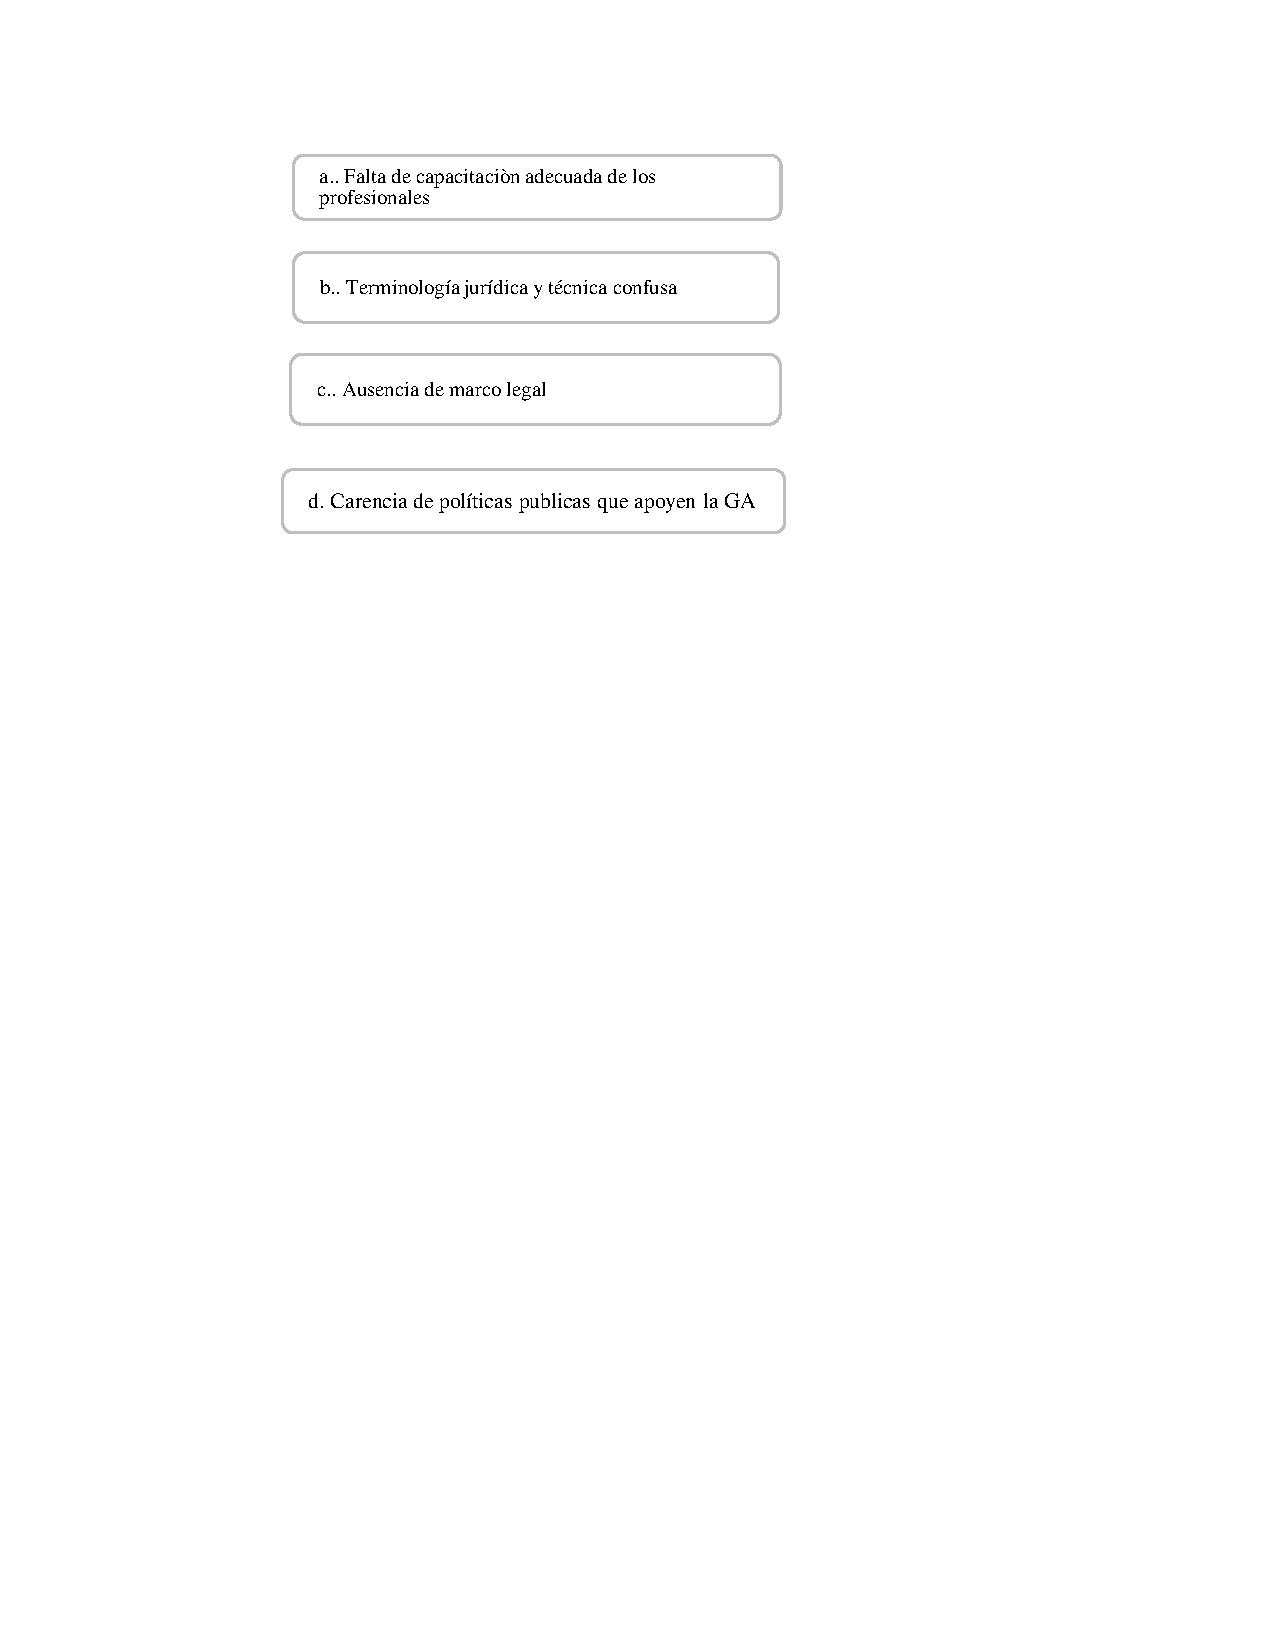
\includegraphics[width=0.85\columnwidth]{imagenes/barrashorizontales.pdf}
\caption{Principales problemas para la implementación de la gobernanza algorítmica}
\label{barrashorizontales}
\end{figure} 


\subsubsection{Falta de capacitación adecuada}

La automatización de las leyes ha venido ocurriendo paulatinamente desde hace una década debido a la convergencia de las leyes y la tecnología digital. Desgraciadamente, la tecnología avanza más rápidamente que el derecho y, en consecuencia, en este momento existe una discordancia entre abogados e ingenieros de software. Si esta discordancia no se atiende, pronto tendremos una sociedad caóticamente legislada por programas escritos por ingenieros de software, que los abogados no entienden plenamente. Este tema lo estudiamos en el capítulo \ref{ngenieriía de software para la Gobernanza Algorítmica (ISGA)} Aclaramos, sin embargo, que uno de los principales inconvenientes es que la tecnología para automatizar leyes se encuentra casi preparada, pero carecemos de profesionales que la puedan implementar correctamente. Actualmente tenemos abogados expertos en leyes que poco saben de programación e ingenieros de software expertos en programación que poco saben de leyes; es decir, no tenemos profesionales que dominen ambos temas. En el capítulo \ref{ngenieriía de software para la Gobernanza Algorítmica (ISGA)} proponemos la creación de la disciplina ISLA (Ingeniería de Software para Leyes Automáticas) y analizamos, desde la perspectiva del Derecho, las habilidades que los expertos en esta disciplina deben adquirir.

\subsubsection{Terminología jurídica y técnica confusa}

Los avances tecnológicos nos ponen, como siempre, frente a nuevos desafíos. El Derecho y la Tecnología hacen uso de un vocabulario específico con sus propios conceptos. El lenguaje jurídico, en lo particular, es un lenguaje técnico que otorga a muchas de las palabras de uso común un valor propio dentro del sistema y, además, crea sus propios términos. Por ejemplo, en el ámbito legal, el contrato inteligente es uno de los conceptos más importantes y, al mismo tiempo, más complicado de dilucidar. Uno de los mayores inconvenientes es la discordancia que existe entre el vocabulario legal y el informático que genera confusión y equivocaciones. El problema es que algunos términos tienen significados diferentes en estas disciplinas; por ejemplo, para un abogado “ejecución de un contrato” significa la firma del contrato, mientras que para un ingeniero de software significa la activación del código de computadora que se encarga de realizar el contrato automáticamente. Las principales complicaciones se fundan en cuestiones semánticas que son necesarias  aclarar para evitar futuros contratiempos en la puesta en marcha de la GA.

\subsubsection{Ausencia de marco legal }

La gobernanza algorítmica aún no se encuentra regulada en Argentina. Entendemos que la presencia de un marco regulatorio adecuado es fundamental para otorgarle seguridad jurídica y para reducir el nivel de incertidumbre creado en su entorno. 

El encuadre jurídico de la GA puede estar constituido de acuerdo a una o varias de las siguientes opciones:

\begin{itemize}
    \item Legislación existente: se aplican las mismas leyes que la gobernanza tradicional.
    \item Modificación de la legislación existente. Necesidad de cambio en las normas existentes para adaptarla a la gobernanza algorítmica.
    \item Legislación o régimen jurídico específico. El marco regulatorio no es suficiente para implementar la GA. Se requiere el dictado de una normativa especial. 


Al ser una disciplina novedosa, en Argentina, la GA nunca fue abordada en su totalidad dentro del contexto jurídico. Menos aún legislada completamente. En algunas situaciones se crearon normas especiales (por ejemplo, la ley de firma digital n° 25.506). En otras ocasiones se aplicaron o modificaron las mismas normas que la gobernanza tradicional (por ejemplo, el artículo 1105 del Código Civil y Comercial de la Nación. que regula a los contratos electrónicos), \footnote{El Código Civil y Comercial de la Nación prevé en su artículo 1110 que en los contratos a distancia, como es el caso de los contratos electrónicos, el consumidor tiene el derecho irrenunciable de revocar su aceptación, dentro de los diez (10) días computados a partir de la celebración del contrato.} En otros países, en cambio, se regula mediante disposiciones específicas como el Código Francés que contiene una sección especialmente para la contratación electrónica . \footnote{En la sección 1, subsección 4, artículos 1125 a 1127 )Sub-section 4 Special Provisions Governing Contracts made by Electronic Means8 Art. 1125 –Electronic means may be used to make available contractual stipulations or information about property or services.  \url{https://www.trans-lex.org/601101/highlight_1125/french-civil-code-2016/\#head_7}}


El sistema jurídico argentino es heredero de la tradición continental. \textcolor{blue}{La característica principal que lo distingue (por ejemplo, del sistema anglosajón) es la codificación de sus leyes.}

%La tradición continental se caracteriza por el recurso de %la codificación.

Surge a partir de ciertos presupuestos que pueden ser resumidos en las siguientes dos proposiciones: a) El legislador / codificador puede prever todas las futuras situaciones de la vida de las personas sujetas a la ley y dar una respuesta anticipada a todos los futuros conflictos que, entre ellas, o entre ellas y el gobierno, pudieran surgir. En otras palabras, el valor justicia es decidido por el legislador (que en una democracia se identifica con el pueblo) y sus manifestaciones concretas respecto de casos específicos pueden ser conocidas (o creadas) antes de que los conflictos (o casos) tengan lugar. Lo que es justo puede ser decidido en abstracto, antes de que ocurran los hechos del caso. b) El derecho (el Código) se expresa mediante un texto que pone de manifiesto la voluntad democrática del pueblo. Ese texto es claro y completo, y debe ser aplicado por los jueces a los casos que se les presenten con máxima fidelidad a la voluntad del legislador, que previó esos casos. 

Es evidente que los avances tecnológicos son imprevisibles y, según nuestra opinión, el derecho argentino, basado en el derecho continental (cuyas normas están contenidas en cuerpos legales (Códigos) unitarios, ordenados y sistematizados), no es lo suficientemente flexible y adaptable para facilitar y ayudar a la regulación de la gobernanza algorítmica. El sistema continental complejiza su implementación por la necesidad de seguir un proceso complicado de reforma. La obra de la codificación es, por sí misma, difícil ya que importa articular un sistema de solución para numerosos casos muy diferentes, que involucran opiniones e intereses también disímiles, que hay que armonizar. Este sistema debe ser equilibrado, para que la colisión de derechos individuales y la que pueda producirse entre estos últimos y los derechos colectivos permita la convivencia social.  Esta tarea es doblemente difícil en las sociedades del siglo XXI, porque todo cambia a ritmo acelerado y la diversidad prolifera.\footnote{Ricardo Luis Lorenzetti, Introducción al Código Civil y Comercial }  Las innovaciones tecnológicas son las principales causas de las continuas transformaciones.

El sistema anglosajón o \textit{common law} (compuesto por un conjunto de principios y reglas de derecho fijados en las decisiones judiciales -y no solo en las normas legislativas), tal como afirma la doctrina jurídica de países como Inglaterra y Gales, no es tan rígido y, por lo tanto, proporciona una plataforma ideal de innovación sin necesidad de reformar la ley estatutaria.

\textbf{Carencia de políticas públicas que apoyen la GA}

La aplicación de las leyes automáticas supone el manejo de una gran cantidad de información (datos) durante el proceso para obtener un resultado. Por ejemplo, en un proceso judicial, el juez debe analizar los casos presentados en tribunales, interpretando y haciendo valer la legislación aplicable al procedimiento correspondiente. En su labor, debe estudiar y comprender extensos volúmenes de datos. Sabemos que existen cuestiones donde son necesaria la intervención de un humano. En los casos más objetivos y exactos puede suplantarse. En la gobernanza tradicional, el juez puede asimilar determinada cantidad de información y, aunque sean incompleta, dar su veredicto de acuerdo a lo que tenga a su alcance. Mientras que la gobernanza algorítmica puede llegar a procesar extensa cantidad de información mediante el uso de tecnologías como IA, Big Data, Legislación legible por máquina. Por lo tanto, en los países que han invertido en tecnología y, por ende, la tecnología se encuentra más desarrollada, el veredicto será más justo, rápido y eficiente, es decir, menos posibilidad de cometer errores. 

\begin{figure}
\centering
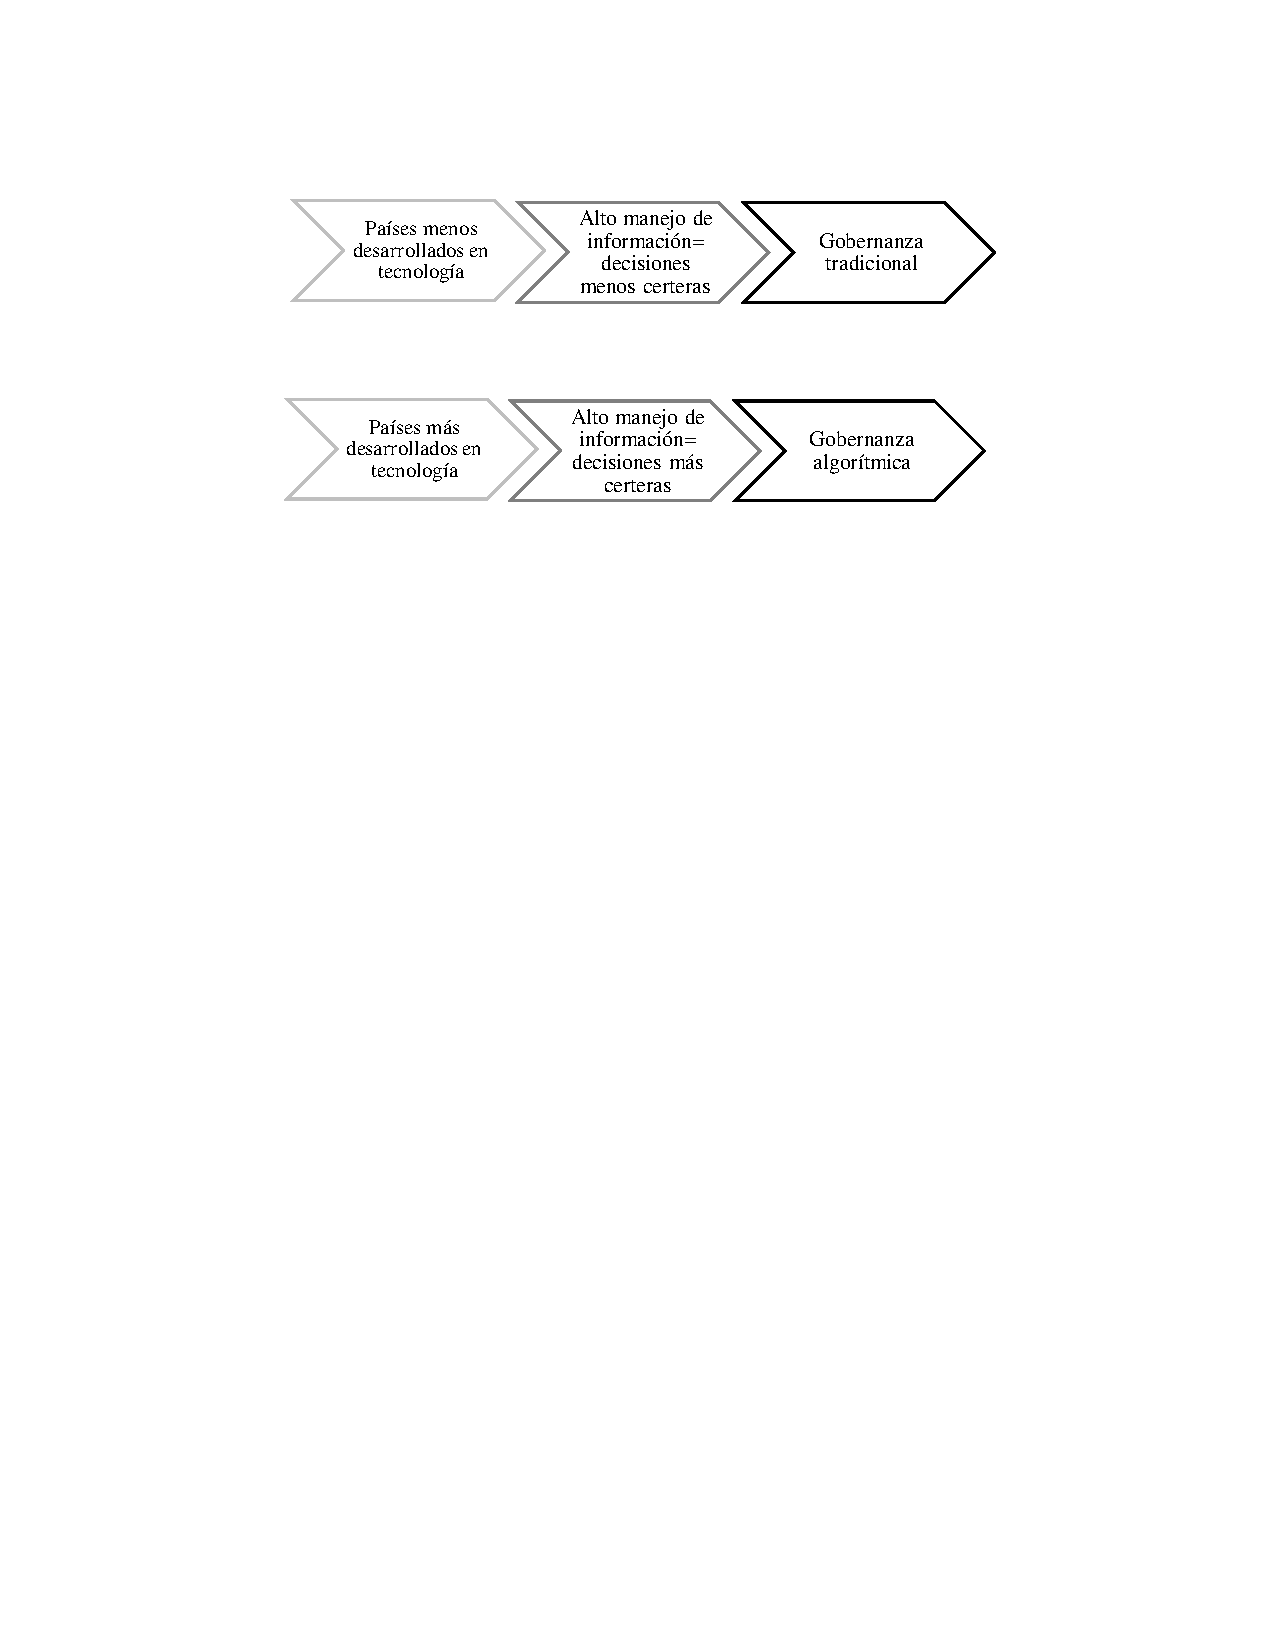
\includegraphics[width=0.85\columnwidth]{imagenes/dosflechas.pdf}
\caption{ Algunas diferencias entre la Gobernanza tradicional y la Gobernanza algorítmica}
\label{dosflechas}
\end{figure} 

El programa es capaz de leer, analizar y procesar en mucho menos tiempo que un humano un caudal de información superior. Entonces, la gobernanza algorítmica va a depender del grado de desarrollo de la tecnología digital en un país. Entre más avanzado se encuentre en un determinado país más información tendrá y más certeras serán sus decisiones. De ahí, la importancia de políticas públicas de innovación tecnológica implementada por los Estados en todos los niveles (nacional, provincial, municipal). 

Resumiendo, consideramos que para incorporar la gobernanza algorítmica en Argentina es conveniente que su implementación sea gradual. Si bien la GA está casi dispuesta para ponerse en práctica a nivel técnico, aún no se encuentra preparada para su total utilización. Es importante resaltar que la brecha entre la GA y la gobernanza tradicional no se puede cerrar sin inversión en tecnología y con una regulación acorde. Los Estados que estén más desarrollados en tecnología y adopten buenas estrategias contarán con mayores ventajas frente a aquellos otros que subestimen sus beneficios.



\chapter{Contratos digitales }
\label{Contratos digitales}

\section{Introducción}

Intuitivamente, un contrato es un acuerdo voluntario celebrado entre dos partes con el objeto de obtener un beneficio mutuo. Los contratos han sido utilizados para estipular las reglas de las interacciones comerciales desde tiempos antiguos. Los contratos celebrados y llevados a cabo sin la asistencia de computadoras han sido ampliamente documentados y comprendidos, al menos por la comunidad jurídica. Por ejemplo, se pueden rastrear hasta el Libro 11 de Las Leyes de Platón\footnote{Translated by Benjamin Jowett, Laws by Plato, Global Grey Ebooks Translated by Benjamin Jowett, 2018.}  y el versículo 282 del Corán\footnote{A. Y. Ali, The Meaning of The Holy Quran, I.D.C.I Islamic Dawah Centre International, 2010.} Sin embargo, la reciente adopción de la tecnología informática en la creación de contratos automatizados exige una seria revisión de lo que hasta ahora entendemos por contratos. Usamos el término tecnología informática para referirnos a dispositivos de hardware (por ejemplo, computadoras portátiles, teléfonos móviles, impresoras y cajas Wifi), software (por ejemplo, Windows, aplicaciones de telefonía móvil y lenguajes de programación) y comunicación de Redes como Internet. Como escritura abreviada, utilizaremos el término tecnología. Dado que actualmente esta tecnología es principalmente digital, algunos autores prefieren emplear el término tecnología digital. Además, debido a que la mayoría de las personas utiliza computadoras y tecnologías de la comunicación para enviar y recibir información (por ejemplo, notificaciones de Facebook y mensajes por WhatsApp) algunos autores prefieren el término Tecnologías de la Información y la Comunicación (TIC). En este trabajo, tomamos los términos tecnología informática, tecnología digital y TIC como sinónimo. Asimismo, bajo el término Internet englobamos páginas web y plataformas como Facebook, Twitter y Bitcoin. Algunos autores se refieren a Internet como la web.

La tecnología informática se puede utilizar para automatizar diferentes etapas del contrato. Sin embargo, el enfoque de este documento es la automatización de la ejecución real del contrato por medio del código de computadora. No discutimos los sistemas de bases de datos que se utilizan para automatizar el almacenamiento y la recuperación de documentos, utilizados para redactar contratos que se ejecutan manualmente.\footnote{Emptoris Contract Management, “Introduction to emptoris contract management (10.1.0).” \url{https://www.ibm.com/docs/en/ecm/10.1.0?topic= guide-introduction-emptoris-contract-management},
2021.CMx Contract Management Software, “9 stages of contract lifecycle management.” \url{https://www.contractexperience.com/resources/resources-main.html}, July 2021. Visited on 1 jul 2021.  R. George, “8 tips to optimize service contract lifecycle management.” \url{https:// global.hitachi\-solutions.com/blog/contract-management}, July 2021. Visited on 1 jul 2021.} La investigación académica dirigida a la automatización de contratos puede remontarse al menos a mediados de la década de 1980 .\footnote{\cite{Minsky1985}Ensuring integrity by adding obligations to privileges} Desde entonces, varias ideas fueron sugeridas por la comunidad de Ciencias de la Computación. A este respecto, los contratos automatizados fueron conocidos como contratos electrónicos, contratos ejecutables, contratos digitales, contratos programables y otros nombres. 
En 1997, Nick Szabo \footnote{\cite{Szabo1997} Smart contracts: Formalizing and securing relationships on public networks} los llamó contratos inteligentes \textit{(smart contracts)}, un término desafortunado que se hizo popular en 2008 cuando la plataforma Bitcoin demostró su potencial en la implementación de sistemas descentralizados .\footnote{Bitcoin Project, “Bitcoin: Bitcoin is an innovative payment network and a new kind of money.” \url{https://bitcoin.org}, 2019.} Decimos lamentable porque, a nuestro juicio, el término genera una confusión innecesaria fuera del ámbito informático. 
 
En primer lugar, no hay nada inteligente en los contratos implementados en las plataformas blockchains como Bitcoin 

\footnote{Bitcoin Project, “Bitcoin:
Bitcoin is an innovative payment network and a new kind of money.” \url{https://bitcoin.org}, 2019.  [13] N. H. Minsky, “Law-governed systems,” 
Software Engineering Journal 6(5), 1991. [14] Z. Milosevic, A. Josang, T. Dimitrakos, and M. Patton, “Discretionary enforcement of electronic contracts,” in Proc. 6th IEEE Int’l Enterprise Distributed Object Computing Conf.(EDOC’02), pp. 39–50, IEEE CS Press, 2002. [15] H. Ludwig and M. Stolze, “Simple obligation and right model (SORM)-for the runtime management of electronic service contracts,” in Proc. 2nd Int’l Workshop on Web Services, e–
Business, and the Semantic Web(WES’03), 
LNCS vol. 3095, pp. 62–76, 2003. [16] P. Linington, “Automating support for e–business contracts,” Int’l 
Journal of Cooperative Information Systems 14, pp. 77–98, Jun-Sep. 2005.[17] C. Molina-Jimenez, S. Shrivastava, and M. Strano, “A model for checking contractual compliance of business interactions,” IEEE Trans. on Service Computing 5(2), pp. 276-289, 2012.}
 


Ethereum\footnote{Ethereum Foundation, “Ethreum: Blockchain app platform.” \url{https://www. ethereum.org}, Visited 23 Oct 2017 2018.}  e Hyperledger \footnote{Hyperledger, “Hyperledger fabric.” \url{https://hyperledger-fabric.readthedocs.io/en/release-1.1/}, 2018.  o en sus predecesores.} \footnote{\cite{Minsky1991}Law-governed system.}
Todos ellos se realizan como código de computadora convencional escrito por los programadores para ejecutar algunas acciones (por ejemplo, transferir N dólares de Alice a Bob) cuando se cumplen determinadas condiciones (por ejemplo, el vencimiento del plazo de pago).

En segundo lugar, hay argumentos planteados por abogados que sostienen que la palabra contrato es inadecuada: un examen completo de los usos de estos fragmentos de código revela que algunos de ellos no son contratos tal como los conciben los profesionales del Derecho .\footnote{\cite{Kieron2017}Smart contracts– dumb idea} En realidad, algunos autores observan (ver por ejemplo) \footnote{\cite{Christopher2019} Smart contract templates: legal semantics and code validation} que existe un desajuste entre la terminología utilizada por abogados y el utilizado por los informáticos. Por cierto, en lenguaje legal ejecutar un contrato significa firmar o suscribir un contrato mientras que en lenguaje técnico significa ejecutar el código informático que implementa el contrato. En este estudio, utilizaremos el término \textbf{contrato digital}.

Para arrojar un poco de luz a la confusión sobre los contratos automáticos, y con la intención de ayudar tanto a la comunidad del derecho como a la informática, proporcionamos una categorización de los contratos existentes de acuerdo con el grado de automatización que utilicen en la etapa de cumplimiento.

Además del grado de automatización, los contratos se pueden clasificar desde otras perspectivas. En consecuencia, se han desarrollado una serie de vectores para categorizarlos. Mencionamos brevemente algunas que están directamente relacionados con el tema de la automatización. Existen contratos bilaterales y multilaterales; además, un contrato puede desarrollarse de manera centralizada (tercero de confianza) o totalmente descentralizado (en una cadena de bloques); también podemos clasificar el contrato de acuerdo con el tipo de firmas que utilizan (manuscritas o electrónicas) y con el grado de intrusión (seguimiento o exigibilidad/ cumplimiento). Creemos que esta discusión adicional coloca a este trabajo en un contexto global.

Una característica destacada de este estudio es que explicamos nuestras definiciones y los argumentos con la asistencia de ejemplos y diagramas de flujo que muestran gráficamente el ciclo de vida de los contratos. Creemos que los mismos ayudarán a los lectores que no están familiarizados con la tecnología informática a apreciar la tecnología que sustenta los contratos automatizados y evaluar sus implicaciones legales, por ejemplo, para determinar de manera informativa si un determinado contrato automatizado cumple con los requisitos para ser declarado un contrato legal.


\section{Automatización de contratos y terminología}

Las ventajas de realizar negocios en línea y los avances recientes en la tecnología informática han motivado a los ingenieros informáticos a implementar contratos que en mayor o menor medida son exigibles automáticamente. Como resultado, actualmente tenemos una gran variedad de contratos con diferentes características. Estos contratos se pueden dividir en dos grandes categorías según el grado de automatización: contratos no automáticos y contratos automáticos. Dentro de la categoría de contratos no automáticos, agrupamos a los contratos tradicionales normalmente registrados en papel, en un idioma natural (por ejemplo, en inglés). Son redactados por abogados y realizados y ejecutados sin signos de automatización. Dentro de la categoría de contratos automáticos, agrupamos a los contratos que se ejecutan parcial o totalmente de forma automática; esto significa que algunas o todas sus operaciones son ejecutadas por medio de código de computadora. Los contratos automáticos están escritos por programadores informáticos (también llamados ingenieros de software) en lenguajes de programación (por ejemplo, Solidity) y son el resultado de la reciente convergencia del derecho y la informática, como explicamos en el capítulo XX. Al tratarse de una tecnología emergente aún no se comprende bien y, además, están deficientemente documentados. En la Sección XX mencionamos que los contratos automáticos se conocen bajo diferentes nombres; en este artículo utilizaremos el término “contratos digitales” para referirnos a ellos. Justificaremos nuestra elección en la Sección  X. Las categorías de contratos automáticos y no automáticos a su vez, se pueden dividir en subcategorías. Para hacerse una idea, podría ser útil observar la Fig. 1, que muestra una descripción general de la categorización de los contratos.



Esta figura \ref{llavescontratos}

\begin{figure}
\centering
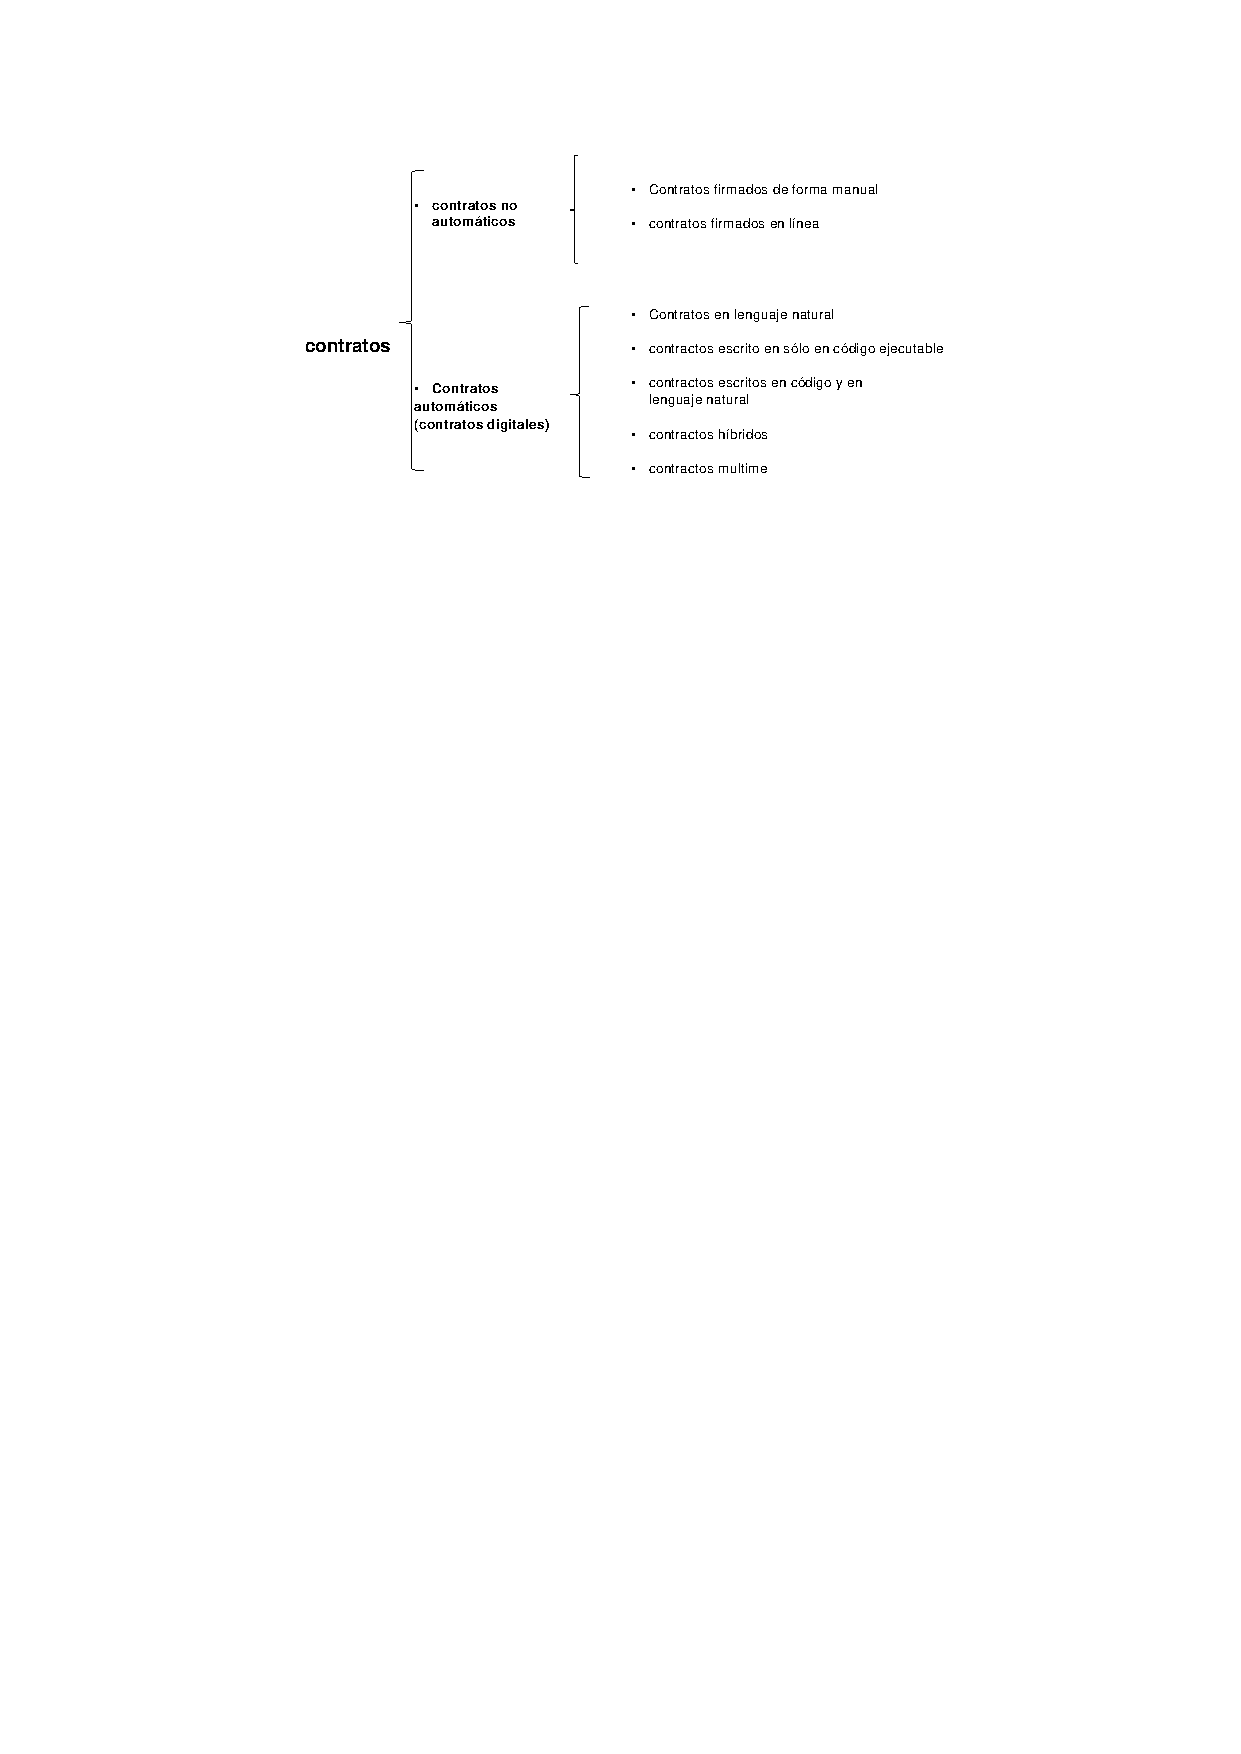
\includegraphics[width=0.85\columnwidth]{imagenes/llavescontratos.pdf}
\caption{Categorías de contratos desde la perspectiva de la automatización}
\label{llavescontratos}
\end{figure} 

Discutiremos cada categoría en profundidad, en secciones posteriores; siendo por el momento suficiente entender que los contratos no automáticos son redactados por abogados y exigibles legalmente mientras que, los contratos automáticos son implementados por ingenieros informáticos y aplicados por un código informático. Sin perjuicio de algunas diferencias en la forma de concebir los contratos, el trabajo de los abogados y de los ingenieros informáticos se complementa e idealmente, debe realizarse en estrecha colaboración. Desafortunadamente esta tarea no es tan sencilla. Los abogados consideran que la automatización de contratos es difícil de entender, mientras que los ingenieros informáticos luchan por comprender qué es un contrato legal. Una de las principales dificultades es el desajuste entre los lenguajes especializados que utilizan los abogados y los ingenieros informáticos, como se explica más adelante. Para mencionar un ejemplo, el término contrato y la terminología relacionada que se utiliza para describir el ciclo de vida de un contrato tiene un significado diferente para los abogados e ingenieros informáticos. Para arrojar algo de luz sobre la confusión, discutiremos el ciclo de vida de los contratos no automáticos y luego la que corresponde a los contratos automáticos. También compararemos y relacionaremos entre sí la terminología utilizada por abogados e ingenieros informáticos. Creemos que la comparación puede ayudar a los abogados a colocar los contratos utilizados en Internet en un marco jurídico. Por ejemplo, les ayudará a determinar categóricamente qué contratos utilizados en Internet cumplen con todos los requisitos para ser considerados contratos legales y cuáles no.

\subsection{Contratos no automáticos y terminología legal}

En el contexto legal, un \textbf{contrato} es un acuerdo formal entre dos partes. Por formal, nos referimos a que el acuerdo cumple con todos los elementos que el ordenamiento jurídico del lugar de formación del contrato requiere para que dicho acuerdo sea exigible legalmente. Dado que estos contratos involucran solo a dos partes, se denominan \textbf{contratos bilaterales}. Hay contratos celebrados entre más de dos partes (llamados \textbf{contratos multipartes}). En este documento no tratamos estos últimos porque su automatización es mucho más compleja que los contratos bilaterales. Las partes que celebran un contrato y se obligan legalmente se denominan \textbf{firmantes}. Para facilitar la explicación en los ejemplos de contrato que mostramos en este trabajo, a los firmantes los llamamos Alice y Bob. Representan a dos seres humanos que se comprometen con esos contratos, ya sea a título personal o como representantes de sus respectivas empresas.


Esta figura \ref{cuadrocontratos1}

\begin{figure}
\centering
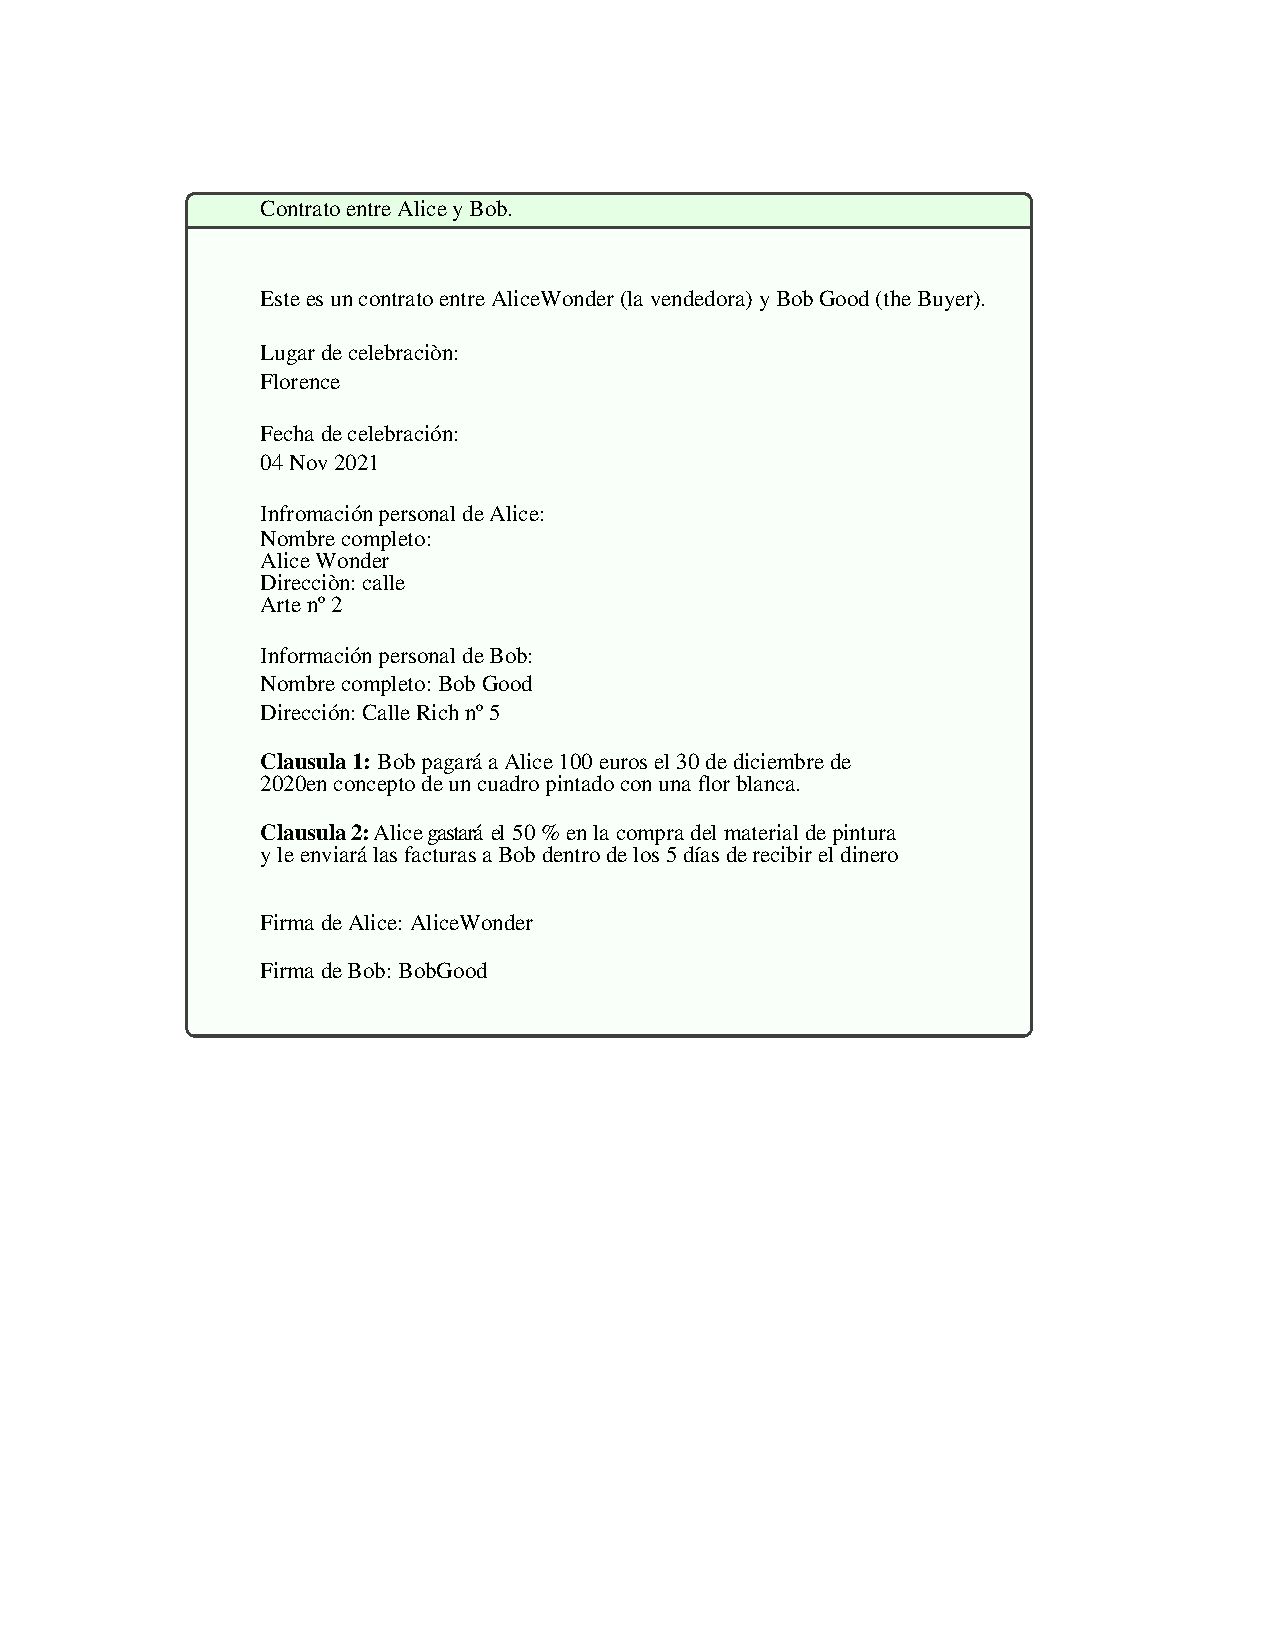
\includegraphics[width=0.85\columnwidth]{imagenes/cuadrocontratos1.pdf}
\caption{Contrato escrito en inglés y firmado manualmente por Alice y Bob}
\label{cuadrocontratos1}
\end{figure} 

Se debe tener en cuenta que alguna doctrina utiliza los términos contratos y acuerdos indistintamente. Sin embargo, hablando estrictamente, en contextos legales no son equivalentes. Los acuerdos se consideran como arreglos informales que no son  exigibles legalmente [20].

Los contratos juegan un papel central en las interacciones humanas, ya que son el instrumento legal más comúnmente utilizado para regular las relaciones comerciales de las personas. Sin embargo, para ser considerado legal, un contrato debe satisfacer algunos requisitos que dependen de la jurisdicción bajo la cual se forman. Actualmente, en el mundo existen diferentes familias jurídicas: como el Derecho Civil, el\textit{Common Law}, el Derecho Consuetudinario\footnote{\cite{Mathias2016}Varieties of legal systems: towards a new global taxonomy} , cada uno con sus propias características. En este trabajo vamos a centrarnos principalmente en el derecho civil, y mencionar el derecho consuetudinario solo para enfatizar que existen ciertas particularidades que los informáticos deben tener en cuenta a la hora de implementar los contratos automáticos.

\subsubsection{El Common Law y el Derecho Civil}

El Derecho Civil (también conocido como derecho continental) surgió en Europa y deriva del derecho romano. Se utiliza en países continentales europeos como Francia, España y Portugal; y en la mayoría de países latinoamericanos, como México, Argentina y Brasil. Aunque los códigos civiles de los diferentes países no son homogéneos, poseen ciertas características que son comunes a todos ellos. Por su parte, el common law se originó en Inglaterra durante la Edad Media y se aplicó dentro de las colonias británicas. En la actualidad, se utiliza en Gran Bretaña y en otras ex colonias británicas como los EE. UU.

\footnote{BerkeleyLaw, ''The common law and civil law traditions.'' \url{https://www.law.berkeley.edu/wp-content/uploads/2017/11/CommonLawCivilLawTraditions.pdf}, Nov. 2017. Visited on 21 Aug 2021. World Bank, ''Key features of common law or civil law systems''

\url{https://ppp.worldbank.org/public-private-partnership/legislation-regulation/framework-assessment/legal-systems/common-vs-civil-law}, 2020. Visited on 8 Aug 2021.} 

Las siguientes son las principales características del sistema de derecho civil \footnote{Idem 14}.


\begin{itemize}
    \item Es un sistema codificado debido a que la aplicación de la ley se basa en códigos legales. Un código es un conjunto de leyes sobre un tema en particular (por ejemplo, materia contractual) que intenta anticipar de manera integral todas las posibles cuestiones que los ciudadanos pueden presentar ante los tribunales. Una característica destacada de los códigos es que son documentos (por ejemplo, libros impresos o documentos en línea) organizados sistemáticamente en secciones y artículos numerados que dictan los procedimientos y sanciones aplicables para cada delito. Por ejemplo, el Subtítulo 1 del Código Civil francés de 2016  se refiere a los Contratos. El Capítulo 1 del Subtítulo 1 se denomina Disposiciones Introductorias y trata de la formación de los Contratos. El artículo 1101 se incluye dentro del Capítulo 1 y define al contrato según el Código Civil Francés de 2016.
    \item	Los jueces trabajan dentro de un marco de leyes codificadas. Su responsabilidad principal es determinar, sobre la base de los hechos que se le presenten, qué código y qué artículo o artículos se aplicarán para resolver la cuestión jurídica que se le plantea. Es decir, la tarea principal de los jueces es interpretar y aplicar la ley contenida en su mayoría en un código para cada caso concreto.

    \item El derecho civil se basa en la teoría de la separación de poderes, según la cual la función del legislador es legislar, mientras que los jueces son los encargados de aplicar la ley.

    \item Cuando se presenta un caso, el abogado de derecho continental tomará como marco jurídico, las normas contenidas en una legislación. Luego, se basará en razonamientos y consideraciones sobre las particularidades del caso.

    \item Los contratos son prescriptivos e inflexibles porque su formación está determinada por el marco legal plasmado en los códigos legales, como la sección de Derecho de los Contratos del Código Civil Francés.

    \item En Derecho Civil, los contratos son acuerdos que unen la voluntad de los firmantes. Por lo tanto, estipulan compromisos consensuales.
\end{itemize}


Esta figura \ref{tablacontratos2}

\begin{figure}
\centering
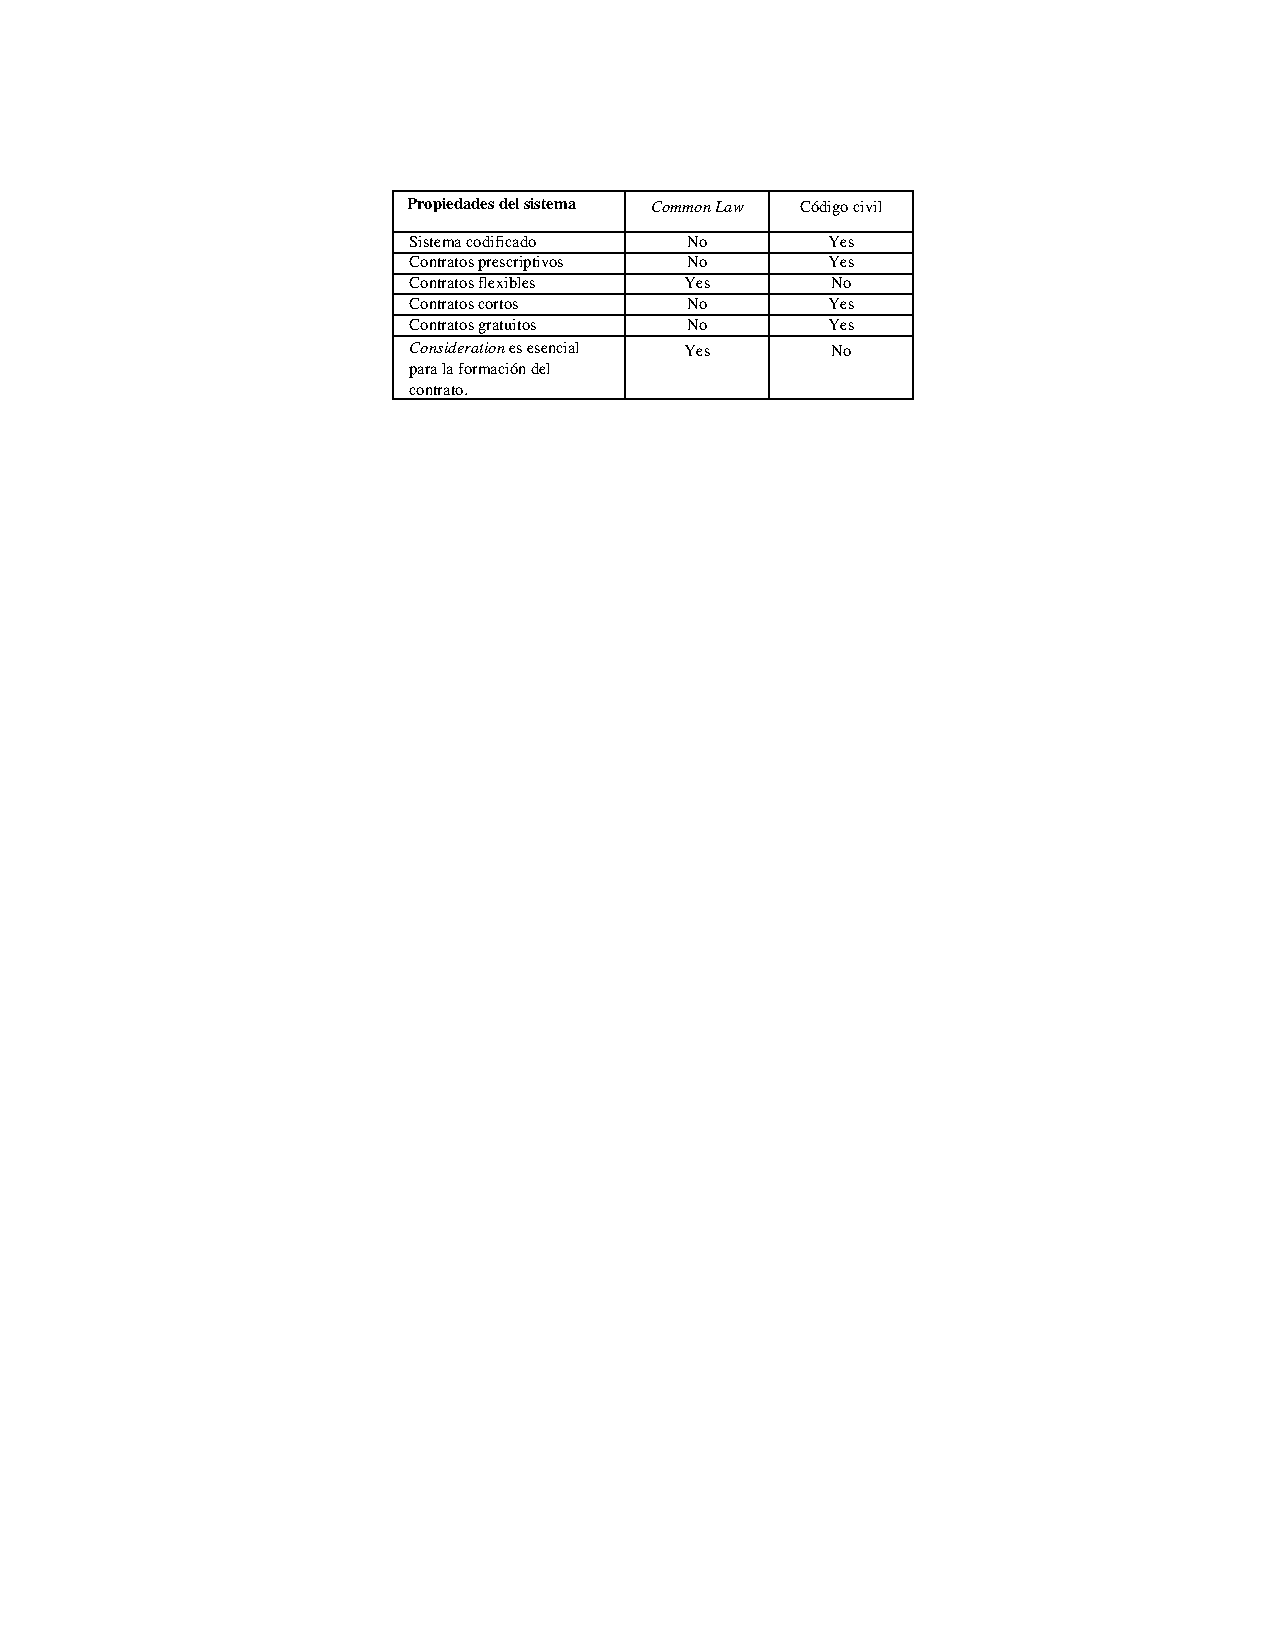
\includegraphics[width=0.85\columnwidth]{imagenes/tablacontratos2.pdf}
\caption{Algunas diferencias entre el Common Law y el Derecho continental.}
\label{tablacontratos2}
\end{figure} 

Relevante para nuestro trabajo son las siguientes características del sistema del \textbf{Common Law} .

Es un sistema no codificado, como tal, no existen códigos organizados sistemáticamente como en el Código Civil Francés .\footnote{\cite{JohnCart2016}French civil code 2016}



\begin{itemize}
    \item Se sustenta en gran medida en precedentes que son resoluciones previas tomadas por los jueces. Significa que las decisiones judiciales se toman sobre la base de casos similares que ya han ocurrido, en lugar de conductas anticipadas y documentadas en artículos de códigos. Por ejemplo, el Código Civil Francés.

\item En el common law, a diferencia del derecho continental, no existe un marco normativo amplio sino que los jueces se encargan, a través de los conflictos particulares, de construir un sistema que debe ser respetado por los ciudadanos. Es decir, se da a los jueces la tarea principal de crear la ley.

\item Un abogado de common law comienza con el caso real y lo compara con otros casos iguales o similares que hayan sido tratados por los jueces en casos anteriores, y a partir de estos precedentes relevantes, la regla legalmente vinculante está determinada por medio de inducción.

\item Amplia libertad de contratación. En general, el Common Law es menos prescriptivo que el Derecho Civil. Por lo tanto, existe amplia libertad en la formación de los contratos. En consecuencia, los contratos deben incluir detalles en lugar de solo referirse a códigos y artículos como en el Derecho Civil. De esta manera los contratos son más flexibles, pero más extensos que en el Derecho Civil.

\item Los contratos son siempre onerosos —cada una de las partes recibe un beneficio del otro como contraprestación. A diferencia del Derecho Civil, no existen los contratos gratuitos donde solo una de las partes proporciona un beneficio a la otra sin esperar ni recibir nada a cambio.

\item En los contratos de derecho anglosajón, la consideration es obligatoria porque el contrato se concibe como una relación de intercambio, en consecuencia, la mera voluntad de los signatarios no es suficiente para el cumplimientode un contrato.    
    
\end{itemize}

La Tabla 1 resume las principales diferencias y similitudes del Common Law y del Sistema de Derecho Civil. Es necesario tener en cuenta que la atención se centra únicamente en las características relacionadas con el contrato que podrían tener correspondencia con la implementación de contratos automáticos. Volvemos a este tema en la Sección 7.

\subsubsection{Las tres fases del ciclo de vida del contrato en el Derecho Civil}


Para entender el proceso de contratación desde la perspectiva de un abogado, analizamos el ciclo de vida de un contrato e identificamos sus fases (también llamadas etapas o momentos). Para ordenar la discusión, tomemos los contratos de Derecho Civil. En esta sección nos referiremos a artículos del Código Civil Francés de 2016 . El análisis de las etapas proporciona sólo un marco para entender el problema sin tener en cuenta las particularidades de cada contrato individual. En general, existen tres fases en el ciclo de vida de un contrato:


\begin{enumerate}
    \item Formación 
    \item Cumplimiento
    \item Terminación   
\end{enumerate}

Utilizaremos el diagrama de flujo que se muestra en la Fig. 3 para explicar sus relaciones. La figura muestra el ciclo de vida de un contrato de Derecho Civil entre Alice y Bob. Excluye las tratativas preliminares de la fase de negociación. Alice acepta o rechaza las ofertas de Bob. Estos contratos son utilizados por proveedores y vendedores que operan bajo la modalidad "tómalo o déjalo" (take it or leave). Dicho sea de paso, este tipo de contratos son muy utilizados actualmente por grandes proveedores de la nube que ofrecen servicios a pequeños consumidores de la nube como, por ejemplo, a individuos que normalmente no tienen poder de negociación. Los grandes proveedores de la nube suelen ser reacios a negociar sus términos y condiciones. A los consumidores se les presentan los contratos estándar de los proveedores. Estos consumidores sólo tienen la opción de presionar la tecla aceptar o salir, sin ninguna oportunidad de negociación.\footnote{\cite{WKuan2013}“Negotiated contracts for cloud services” } 

\textbf{Fase de formación:} Como se muestra en la Fig. 3, la fase de formación incluye subetapas negociación y conclusión y tiene por objeto la formalización del contrato que no se alcanza cuando se abandona la negociación. La negociación preliminar comenzó a ser considerada por la doctrina jurídica, a fines del siglo XIX (ver los estudios de von Ihering).  Sin embargo, alcanzó un mayor desarrollo durante el siglo XX. En términos legales, la negociación es un proceso no vinculante llevado a cabo por dos posibles contratantes con la intención de llegar a un acuerdo sobre los términos y condiciones a incluir en un contrato. Esta es una fase de disidencia, prueba y error, reservas y discusión donde su suspensión o ruptura, en principio, constituye algo admisible y natural que no es anormal o ilegal. El requisito esencial para la existencia de un acuerdo es el consentimiento, no las tratativas preliminares o la discusión previa. Sin embargo, las negociaciones cobran relevancia si conducen a la formalización del contrato. Por ejemplo, ayudarán a interpretar el contrato. Asimismo, si el contrato se frustra, las negociaciones pueden generar responsabilidad a cada parte en función de los daños causados a la otra [?]. Usamos la Fig. 3 para aclarar estos puntos.
\begin{itemize}
    \item \textbf{ Oferta:} La negociación comienza cuando una de las partes presenta una oferta a la otra. El Código Civil francés  estipula que una oferta expresa la voluntad del oferente y que una oferta es vinculante si el destinatario la acepta (artículo 1114). El Código Civil y Comercial de la Nación se orienta en igual sentido. VERIFICAR. En algunas situaciones, una oferta es el resultado de negociaciones preliminares (iter negocial). Otra palabra comúnmente utilizada en el lenguaje jurídico para referirse a la oferta es la “promesa”. La parte que presenta la oferta se denomina oferente o promitente y la parte que recibe la oferta se llama el destinatario de la oferta o el prometido. En el ejemplo de Fig 3, Bobs es el oferente y Alice es la destinataria de la oferta. Bob le presenta la oferta a Alice en el recuadro 2.
    \item \textbf{Aceptación:} El Código Civil Francés establece que es la manifestación de la voluntad del destinatario de obligarse en los términos de la oferta (artículo 1118, 1° párrafo). La aceptación es un componente requerido en el proceso contractual. Como se muestra en el rombo 3 de la figura, Alicia tiene dos alternativas cuando recibe la oferta de Bob. Ella puede aceptar la oferta y hacer que el diagrama de flujo progrese al recuadro 5, o rechazarla, y llevar el diagrama de flujo al rombo 4. En el rombo 4, Bob puede mejorar su oferta y hacer que el diagrama de flujo regrese al recuadro 2 donde presenta su nueva oferta a Alicia. Alternativamente, desde el rombo 4, Bob puede decidir abandonar la negociación y hacer que el diagrama de flujo progrese hasta el cuadro 10, que representa el final de la interacción comercial entre Bob y Alice. Una aceptación se vuelve vinculante tan pronto como llega al oferente, antes de este acto, una aceptación puede ser retirada sin consecuencias legales (artículo 1118, 2° párrafo). Las aceptaciones que no se ajusten a la oferta en la negociación, no surtirán efecto; sólo pueden ser consideradas como nuevas ofertas (art. 1118, párr. 3).

    \item \textbf{Formalización o celebración del contrato: } El Código Civil francés \footnote{\cite{Millard2013}“Negotiated contracts for cloud services,” } estipula que un contrato se forma con la reunión de una oferta y una aceptación en la cual las partes manifiestan su voluntad de obligarse (artículo 1113) y se formaliza (concluye) tan pronto como la aceptación llega al oferente (artículo 1121). En la figura, la celebración del contrato tiene lugar en el recuadro 5. La formalización incluye la firma del contrato —si es exigido—, y la iniciación del acuerdo. Por el principio de la libertad contractual, el consentimiento \textit{-consensus— }de las partes produce la perfección del contrato y adquiere fuerza obligatoria con algunas excepciones tales como, aquellos contratos que necesitan formalidades específicas establecidas por la legislación \textit{—ad solemnitatem} (artículo 1172).
\end{itemize}



COLOCAR CUADRO


\section{Fase de cumplimiento o ejecución:} Esta fase se alcanza solo cuando la fase de formación se completa con éxito y se refiere al cumplimiento del contrato.

\textbf{Cumplimiento del contrato:} durante esta fase, se espera que los participantes realicen las acciones necesarias (por ejemplo, hacer una factura o completar el diseño o construcción de un equipo) para cumplir con sus obligaciones según lo acordado en el contrato. En la figura, la ejecución del contrato tiene lugar en el recuadro 6 desde donde el diagrama de flujo avanza hasta el rombo 7. Allí se evalúa el comportamiento de las partes.


\textbf{Incumplimiento de contrato:} En situaciones ideales, las partes actúan según lo estipulado en el contrato y hacen que el diagrama de flujo progrese del rombo 7 al rombo 8. Sin embargo, en situaciones no ideales, el contrato se incumple y el diagrama de flujo avanza de rombo 7 a la casilla 9 donde tiene lugar la ejecución del contrato. Esta situación podría ocurrir cuando los términos de un contrato son violados o ignorados. Es decir, puede suceder cuando una parte no cumple a tiempo, no cumple de conformidad con los términos del acuerdo, o no cumple en absoluto. Cuando se produce el incumplimiento del contrato o se presume, una o ambas partes pueden preferir exigir el cumplimiento del contrato en los términos estipulados, como se muestra en el recuadro 9. En este sentido, el Código Civil francés estipula que la parte con la que no se ha cumplido un compromiso o se ha cumplido de manera imperfecta, puede negarse a cumplir o suspender el cumplimiento de sus propias obligaciones, solicitar el cumplimiento forzado  de la obligación en especie, solicitar una rebaja del precio, provocar la rescisión del contrato o reclamar la reparación de las consecuencias por incumplimiento (artículo 1217).


\textbf{Exigibilidad del contrato:} Se llega a la casilla 9, cuando una de las parte incumple el contrato, la otra parte, lo lleva ante el juez para exigir su cumplimiento. En la práctica, la casilla 9 representa la intervención de un tribunal cuando así lo exige la parte ofendida.


\textbf{Fase de terminación}. Esta fase representa la finalización del contrato. El efecto ideal del contrato es el cumplimiento de las obligaciones asumidas por las partes, que produce la terminación de la relación jurídica. Por ejemplo, un contrato termina cuando el pago ha sido realizado por un comprador y aceptado por el vendedor. La terminación del contrato se verifica en el rombo 8 al que se accede desde la casilla 9 y alternativamente desde el rombo 7. El rombo 8 ofrece distintas opciones: Si el contrato ha terminado, el flujo avanza del rombo 8 a la elipse 10 y llega a la fase de terminación. Por otra parte, si el contrato aún no ha terminado (por ejemplo, todavía hay obligaciones pendientes), salta desde el rombo 8 hasta el recuadro 6, donde continúa la etapa de ejecución o cumplimiento del contrato.

El Derecho civil francés determina que la etapa de terminación pone fin al contrato (artículo 1229) y añade también que en todo caso, puede ser reclamada por vía judicial (Artículo 1227). Un tribunal puede, según las circunstancias, reconocer o declarar la terminación del contrato (artículo 1228). 

Una vez concluida la relación contractual, las estipulaciones acordadas por las partes permanecen en vigor (restitución, reparación de daños, resolución de conflictos y cualquier otra que regule los derechos y obligaciones de las partes después de la terminación). Ciertos deberes y responsabilidades de las partes subsisten después de la conclusión del contrato. Por ejemplo, las obligaciones de no divulgar la propiedad intelectual pueden permanecer en vigor después de la finalización de contrato. La propia legislación francesa prevé algunos supuestos de efectos ulteriores, incluso después del cumplimiento del contrato como por ejemplo, la garantía de evicción (Artículo 1626)

La etapa de formación que se muestra en la Fig. 3 es asimétrica en el sentido de que Alice no tiene poder de negociación Los contratos que resultan de las etapas de formación simétrica donde ambas partes están en condiciones de negociar son también comunes. Como se muestra en la Fig. 4, el ciclo de vida de estos contratos es ligeramente diferente. 

Todas estas cuestiones que mencionamos tienen implicaciones cuando el contrato es ejecutado automáticamente. En la sección XX, lo explicamos con detalle.

\subsection{Contratos automáticos (digitales) y terminología de los ingenieros informáticos}

El contrato que se muestra en la Fig. 2 se puede realizar de forma no automática, es decir, sin utilizar tecnología digital en la fase de cumplimiento. Otra alternativa es convertirlo en un contrato digital que se pueda realizar de forma automática, es decir, un contrato donde  las acciones que tienen lugar en los recuadros 6-8 y 7-9 de la Fig. 3 y la Fig. 4, respectivamente, se realizan sin intervención humana. Como se discutió brevemente en\cite{Christopher2019} y\cite{Monika2019},  los ingenieros en computación usan una terminología para referirse a los contratos digitales que no coincide con la terminología que utilizan los abogados. En esta sección, nos valdremos de los términos empleados por los ingenieros informáticos En el apartado 2.2 relacionaremos los términos que utilizan los abogados y los ingenieros informáticos entre sí.

La figura 5, muestra la conversión del contrato que se muestra en la figura 2 en un contrato digital. Un contrato digital es una pieza de código informático ejecutable que se puede implementar para que  el contrato correspondiente se cumpla automáticamente. Como el código ejecutable representa al contrato, lo llamaremos el código contractual. La Fig. 5 muestra cómo se produce y ejecuta el código ejecutable que implementa un contrato. 

La figura presume que Alice y Bob han aceptado y firmado los términos y condiciones estipuladas por la cláusula 1 y la cláusula 2 de la Fig. 2. Contratan a un abogado para redactar el contrato en el lenguaje natural que se muestra en la figura. 

Alice y Bob contratan a un programador para producir el contrato digital. El programador traduce los términos y condiciones incluidos en el texto en lenguaje natural a un programa codificado (escrito) en un lenguaje de programación, por ejemplo, en Solidity o Python. El código resultante es un contrato digital equivalente al contrato original en Inglés pero ejecutable. Las líneas que se muestran dentro del recuadro dan una idea sobre la representación del contrato en código ejecutable. Estrictamente hablando, estas líneas tienen que ser compiladas (traducidas al lenguaje binario de 0s y 1s que la computadora puede ejecutar) antes de que sean realmente ejecutables, pero estos detalles técnicos son irrelevantes para los objetivos de este trabajo. Así, diremos que el contrato digital realizado por el programador es ejecutable. El programador escribe, implementa y pone en marcha el código del contrato en beneficio de las partes signatarias. Usaremos la Fig. 5 para explicar el proceso que conduce a la implementación y ejecución de un contrato digital. 

El objetivo es dar una idea general de cómo se crean los contratos digitales. No tendremos en cuenta las particularidades del contrato en lenguaje natural o la categoría de contrato digital (ver Fig. ??). La figura asume que Alice y Bob pueden conectarse a Internet desde sus respectivas computadoras y llegar al entorno de ejecución donde los contratos digitales están en funcionamiento.. También se supone que el contrato escrito en inglés ya ha sido celebrado, escrito en papel y firmado bajo firmas holográficas y conforme a una legislación dada, es decir, es un contrato legal. Volvemos al tema de la legalidad de los contratos digitales es la Sección 7.2.

\begin{enumerate}
    \item \textbf{ Contrato escrito en lenguaje natural:} Un abogado es responsable de redactar el contrato que Alice y Bob acordaron. El contrato está escrito en idioma natural, por ejemplo en inglés o español, digamos en una hoja A4, y firmado bajo firmas holográficas.

    
    \item \textbf{ Codificación de contrato digital:} Alice y Bob contratan a un programador para realizar el contrato digital. El programador traduce los términos y condiciones incluidos en el contrato original a un programa codificado (escrito) en un lenguaje de programación, por ejemplo, en Solidity o Python. La intención es producir un contrato digital que sea equivalente al contrato original pero ejecutable. Los errores son comunes en esta etapa, por lo tanto, como se muestra en la figura, el programador normalmente repetirá varias veces los circuitos compuesto por la caja ii y el rombo iii para corregir los errores. Por ejemplo, el recuadro ii muestra que el programador cometió un error cuando codificó la fecha 30/dic/2021. El proceso de corrección de errores se llama “depuración del contrato” e implica probar el contrato digital para asegurarse de que implementa el contrato original. Finalmente, el programador avanza a box IV. Es importante tener en cuenta que algunos errores pueden estar en el texto original y, por lo tanto, pueden requerir la modificación del texto que figura en el recuadro i. Volveremos sobre este tema en la Sección 7.

    
    \item \textbf{ Contrato digital codificado:} el programador, posiblemente después de corregir varios errores, produce un contrato digital que es equivalente al contrato original que se muestra en el cuadro i, ejecutable, libre de errores y listo para su implementación. Las líneas que se muestran en las casillas ii, iii y iv dan una idea de la estructura del contrato expresada en código ejecutable. Estrictamente hablando, estas líneas tienen que ser compiladas antes de que sean ralamente ejecutables, pero estos detalles técnicos son irrelevantes a nivel de discusión de este trabajo. Así, diremos que el contrato digital producido por el programador es ejecutable.


\item \textbf {Contrato digital implementado:} El programador implementa el contrato digital en un entorno de ejecución. Por ejemplo, en una cadena de bloques como Ethereum o Hyperledger. El contrato digital ahora está listo para reaccionar a las acciones enviadas por Alice y Bob desde sus respectivas computadoras (por ejemplo, computadoras portátiles, teléfonos móviles, tabletas, etc.). Decimos que el contrato digital ya está en ejecución. El entorno de ejecución garantiza que el contrato digital esté protegido de alteraciones y permanece operativo cuando la interacción comercial entre los participantes está en marcha. Volvemos a este tema en la Sección 6.1.


\item \textbf {Contrato digital ejecutado:} Alice y Bob ejecutan el contrato digital para interactuar entre ellos. El contrato digital es responsable de cumplir las obligaciones de Alice y de Bob estipuladas en el contrato original
... algunos autores distinguen cinco fases sucesivas y estrechamente entrelazadas: conceptualización, implementación, aprobación, ejecución y finalización  .


\end{enumerate}

\subsubsection{Derechos, obligaciones, prohibiciones y operaciones}

 Desde una perspectiva técnica, un contrato se concibe como un conjunto de cláusulas que estipulan derechos, obligaciones y prohibiciones que se espera que cumplan las partes o firmantes. Los derechos, obligaciones y prohibiciones están asociados al menos con una operación. Una operación es una acción comercial ejecutada por una parte que cambia el estado de desarrollo del contrato.   

Intuitivamente, un derecho es una operación que una parte tiene la facultad de  ejecutar. Una obligación es una operación que se espera que una de las partes ejecute. Finalmente, una prohibición es una operación que una parte no se espera que ejecute. Por ejemplo, en el contrato de la Fig. 2 Bob tiene la obligación de pagar a Alice \$100,00 bajo ciertas condiciones (hasta el 31/12/2021). Para respetar esta obligación Bob necesita ejecutar con éxito a través de algún mecanismo la operación correspondiente "pagar 100,00 a Alice" antes de la fecha límite. En la práctica, los contratos incluyen varias obligaciones. Por ejemplo, un comprador tiene la obligación de pagar y un vendedor la obligación de entregar y la obligación de reembolsar. Por lo tanto, para cumplir con todo el contrato, las partes signatarias deben responder con cada obligación mediante la ejecución de la operación correspondiente: pagar, entregar y reembolsar en este ejemplo. La motivación para utilizar contratos digitales es que automatizan la ejecución de operaciones en cumplimiento de los derechos, obligaciones y prohibiciones estipuladas en el contrato. La ejecución automática libera a las partes signatarias de la molestia de cumplir con las obligaciones correspondientes de forma manual.

Para comprender la ejecución en los contratos digitales, es útil considerar la ejecución de un contrato digital como la ejecución de varias operaciones interrelacionadas donde la ejecución de una de ellas cumple una obligación y puede habilitar o inhabilitar a otras.

Los contratos normalmente incluyen varios derechos, obligaciones y prohibiciones, por lo tanto, involucran la ejecución de varias operaciones interrelacionadas donde la ejecución de una de ellas cumple una obligación y puede habilitar o deshabilitar a otras. Algunos autores consideran cada derecho, obligación y prohibición como un contrato individual. En este modelo, un contrato se compone de uno o más subcontratos interrelacionados.


\subsubsection{Ejecución del contrato}

En los contratos automáticos, las operaciones se ejecutan mediante la ejecución del código ejecutable. La figura 6 muestra la ejecución de una operación de pago. En ella, se supone que en un contrato Bob (el pagador) debe pagar \$100 a Alice (la beneficiaria). La aplicación de Bob está instalada en su computadora portátil y la de Alice está instalada en su teléfono móvil. Además, se asume que el código ejecutable que lleva a cabo la operación de pago está implementado en un lenguaje de programación e instalado en una computadora local, en un servidor en la nube o en una cadena de bloques, estos detalles de implementación son irrelevantes para este estudio.

Para pagar a Alice, la aplicación de Bob ejecuta la operación 'pagar \$100' a través del código ejecutable. Como respuesta, el código ejecutable efectúa la operación y como resultado, la aplicación de Alice recibe una notificación de pago, por ejemplo, el comprobante bancario del pago.

Obsérvese que la Fig. 6 muestra solo la ejecución de la operación de pago. no hay mecanismos digitales establecidos para detectar la falla de Bob para realizar la operación de pago o para exigirle su cumplimiento de forma automática. Esta limitación  se aborda con la ayuda de un contrato digital que se puede implementar para monitorear (ver Fig. 8) o hacer cumplir (ver Fig. 9) la ejecución de las operaciones contractuales. Esta observación conduce a la categorización de los contratos en: contratos de seguimiento o monitoreo y cumplimiento de contratos. La Fig. 7 resume sus principales características.

\subsubsection{Seguimiento o monitoreo de contratos}

El monitoreo o seguimiento de contrato es una técnica en la que se observa de forma pasiva el desarrollo de la ejecución de un contrato digital y se almacena los registros de la operación efectuada por las partes firmantes. El monitoreo es pasivo en el sentido de que no interfiere con el desarrollo del contrato; solo observa y mantiene registros para potenciales exámenes post morten. Por ejemplo, si se plantea una disputa.

La Fig. 8 muestra un contrato digital de monitoreo o seguimiento que puede usarse para monitorear la ejecución de la operación de pago. Nótese que el contrato digital está directamente interrelacionado con el código ejecutable que implementa la operación de pago. De hecho, en la literatura existente, los dos componentes se discuten con frecuencia como uno solo. En nuestra opinión, la separación ayuda a comprender cómo funcionan los contratos automáticos.


 \begin{enumerate}
     \item La aplicación de Bob sitúa la operación "ejecutar pago \$100" en el código ejecutable.

     \item El código ejecutable efectúa la operación y, como resultado, la aplicación de Alice recibe una "notificación de pago", por ejemplo, un recibo bancario.

     \item El código ejecutable proporciona el contrato digital que se encarga de monitorear y registrar la ejecución de la operación de “pago \$100”, iniciada por Bob.

     \item El contrato de monitoreo analiza los registros, determina si la operación "pagar 100" es legal (conformidad contractual) o no y almacena el documento junto con sus resultados (conformidad contractual o incumplimiento de las estipulaciones contractuales) en una base de datos. Los registros acumulados en la base de datos se puede utilizar para realizar un examen post-mortem (fuera de línea) del desarrollo del contrato.

     \subsubsection{. Cumplimiento o exigibilidad del contrato}

La ejecución de contratos es una técnica en la que se observa la ejecución de un contrato digital para observar el desarrollo de un contrato e interferir con la ejecución de operaciones para asegurar que las partes no incumplen el contrato. Como se muestra en la Fig. 9, para ser preventivo, la aplicación necesita operar de manera intrusiva, en lugar de no intrusiva como en el monitoreo de contratos.

En el ejemplo de la figura, se implementa un contrato digital para exigir la ejecución de la operación "pagar 100" que se muestra en la Fig. 6 y en la Fig. 8. El contrato digital es responsable de seguir el desarrollo del contrato y asegurar que la operación ”pago 100” se realiza cuando sea necesario según lo estipulado en el contrato, por ejemplo, dentro del plazo de cumplimiento.

\begin{enumerate}
    \item La aplicación de Bob coloca la ejecución de la operación "pagar 100" en el código ejecutable.

    \item La operación es interceptada por el contrato digital y analiza que el contrato cumpla con las estipulaciones establecidas. Si es así, el contrato reenvía la operación al código que implementa la operación de pago, de lo contrario (si la operación es ilegal) el contrato se descarta la operación de modo que se impida su ejecución.

    \item Cuando la operación "pagar 100" alcanza el código ejecutable, se ejecuta "pagar 100". La aplicación de Alice no necesariamente recibe el dinero real, podría recibir solo una notificación de pago, como se muestra en la figura, por ejemplo, un recibo bancario.

    \item El contrato de ejecución es responsable de asegurar que Bob cumpla con su obligación pagar. En consecuencia, incluye un mecanismo de recordatorio (recordatorio de pago) que es activado cuando el contrato advierte que la solicitud de Bob aún no ha pagado y el plazo para pagar está a punto de expirar. Hay que destacar que el contrato también permite solo la ejecución  de operaciones legales; por ejemplo, no le permitirá a la aplicación de Alice ejecutar una operación de "pago 100" fuera de la ventana de pago, es decir, antes o después de los días de pago pactados.

    A nivel de implementación, el contrato digital es una máquina de estados finitos que sigue el desarrollo del contrato. Sabe con precisión qué operaciones se han cumplido, violados y se encuentran pendientes; como resultado, el contrato es capaz de detener la ejecución de operaciones ilícitas y de exigir el cumplimiento de operaciones pendientes o, al menos, enviar mensajes de advertencia.

    La facultad de exigibilidad depende de las particularidades para ejecutar las operaciones; por ejemplo, un contrato puede exigir el cumplimiento de la operación de "pagar 100" de Bob si se le proporciona dinero por adelantado, como en depósito, o vinculado a las cuentas de Alice a través de alguna API; De lo contrario, el contrato solo puede enviar un mensaje de advertencia a la aplicación de Bob para recordarle la obligación pendiente; Luego, depende de la aplicación de Bob cumplir o violar el contrato.

    Desde la perspectiva del nivel de interferencia que provoca el contrato digital en la ejecución de las operaciones contractuales, los contratos digitales se pueden categorizar en dos clases: seguimiento o monitoreo y cumplimiento o exigibilidad de los contratos, como se muestran, respectivamente, en la Fig. 8 y Fig. 9. La distinción entre monitoreo y cumplimiento es crucial en Lex Cryptographia y fue prevista por Primavera De Filippi [29] y otros autores. Desafortunadamente, ellos no han tomado en cuenta el monitoreo o seguimiento contractual; su enfoque principal está en la aplicación de los contratos.

    \subsection{Grados de automatización}

Nótese que la automatización en el cumplimiento contractual no es binaria (todo o nada), sino una línea que se extiende desde la ausencia de automatización hasta grados crecientes de automatización. Comprender esto como un espectro es útil. De hecho, contratos que, en menor o mayor medida, proporcionar cierto grado de automatización ya están en uso en los negocios en línea actuales. Por ejemplo, los usuarios normalmente firman contratos en línea con el Servicio de Proveedores de Internet para suscribirse a servicios de banda ancha; asimismo, los usuarios obtienen acceso a redes sociales como FaceBook y Twitter luego de firmar contratos en línea que estipulan los términos y condiciones de acceso a la plataforma de la red social, las compras en línea también implican la firma de contratos en línea. Sin embargo, el objetivo es implementar contratos más sofisticados que se pueden utilizar para automatizar la aplicación de la ley según lo previsto en la Lex Cryptographia\footnotesize\cite{PrimaveraAaron2018}  y Computational Law [?], Computable Contracts [?] y Legislaciones legible por computadora  y Contratos sabios . Los avances en la automatización del contrato ha resultado en una gran variedad de contratos que hemos categorizado, como se muestra en la Fig. ??. Discutiremos las subcategorías de contratos automatizados por separado en secciones posteriores.


    \subsection{Comparación de la terminología de abogados e ingenieros de software}

    Una rápida mirada a las Figs. 3, Fig. 4 y Fig. 5 revelarán que no hay consenso entre la terminología utilizada por abogados e ingenieros de software. La identificación de los conceptos legales y técnicos no es directa y en relación de uno a uno. Por ejemplo, ¿la separación de etapas en un contrato no automático como se muestra en la Fig. ??  mp están tan claras en un contrato digital . Además, existen algunos conceptos en los contratos legales, pero no en los contratos digitales y viceversa. Por ejemplo, en los contratos no automáticos, las firmas se colocan simultáneamente sobre el documento de papel, las partes signatarias se encuentran físicamente en la misma habitación; por lo tanto, la noción de vinculación legal simultánea es natural. En cambio, en los contratos digitales, la simultaneidad se pierde porque el contrato se firma de forma remota utilizando protocolos de firma contractuales . Por citar otro ejemplo, en los contratos no automáticos una firma es un componente gráfico, elaborado a partir de alguna sustancia química, en su propio derecho, en la medida en que se puede ver como un componente gráfico que se agrega al documento. Por el contrario, el concepto de firma como componente visible de un documento se desdibuja en algunos contratos automáticos, concretamente en contratos firmados con claves pub-priv. Aquí se puede usar un programa para verificar si un documento está firmado o no por Alice, pero no hay forma de ver la firma de Alice separada de un documento, digamos, antes de los signos o como un componente gráfico del documento firmado. Para explicar estas y otras cuestiones y comparar la terminología utilizada por abogados e ingenieros de software, usaremos el ejemplo de contrato que se muestra en la Fig. 10. El ejemplo fue tomado de  donde también utilizamos el código de Solidity. Hemos omitido algunas de las funciones para simplificar nuestra discusión. 
    
La Fig. 11 muestra el ciclo de vida del contrato del ejemplo de la Fig. 10. Hemos etiquetado las casillas con los términos utilizados por abogados e ingenieros de software.

Analicemos la Fig. 11 desde la perspectiva técnica.

   
    
\end{enumerate}

     
 \end{enumerate}



\begin{itemize}
    \item \textbf{Contrato en lenguaje natural:} El ciclo de vida del contrato digital comienza en el recuadro 8 donde Alice y Bob tienen un contrato escrito en lenguaje natural, como muestra el texto que se muestra en la Fig. 10, presumiblemente redactado por un abogado. Nótese que el texto no está firmado por Alice o Bob bajo firmas holográficas.
    \item \textbf{Codificación del contrato digital}: esta etapa consta de dos pasos: la codificación del contrato digital que tiene lugar en la casilla 9 y la prueba del contrato digital que tiene lugar en el rombo 10. Nótese que, en aras de la simplicidad, la Fig. 5 no muestra la etapa de prueba. La falta de satisfacción de los requisitos de prueba lleva de nuevo al contrato escrito en lenguaje natural (recuadro 8) donde Peter, el programador junto con Alice y Bob revisan el texto del contrato. Aunque no se muestra explícitamente en la figura, es muy posible que el texto del contrato se altere, por ejemplo, para corregir ambigüedades que impiden que Peter escriba un sonido contrato digital.

     \item \textbf{Depuración de contratos digitales} : como se muestra en el lado izquierdo de la figura, el agregado de los pasos 8, 9 y 10 se conoce como depuración de contratos digitales, ya que tiene como objetivo descubrir y eliminar errores (bugs) del código del contrato digital escrito en un lenguaje de programación y del texto del contrato escrito en lenguaje natural. En la práctica, los requisitos de prueba son impuestos por los usuarios del contrato digital (Alice y Bob en este ejemplo). Los requisitos adicionales posiblemente son impuestos por otras partes, como los propietarios del entorno de ejecución donde se desplegará el contrato digital y organismos de normalización como los gobiernos para garantizar el funcionamiento seguro del contrato digital.
     \item \textbf{Implementación del contrato digital: }una vez que el contrato digital cumple con todos los requisitos de prueba, está listo para su implementación en un entorno de ejecución, por ejemplo, en la cadena de bloques Ethereum, como ejemplo particular. En el recuadro 11, Peter, el programador, despliega el contrato digital y lo deja listo para que Alice y Bob lo ejecuten.
     \item\textbf{Ejecución de contratos digitales y cumplimiento de obligaciones:}
     recuadros 12 a 16 representan la ejecución del contrato digital, en la terminología de los ingenieros informáticos. Los derechos, obligaciones y prohibiciones estipulados en el contrato son cumplidas por el contrato digital El código digital permite la ejecución sólo de operaciones que son debe cumplir el contrato. El mecanismo de ejecución utilizado por el contrato digital es similar al que se muestra en la Fig. 9.

     \- El rombo 12 representa el derecho de Alicia a hacer una apuesta y corresponde a la cláusula 3 del texto que se muestra en la Fig. 10. El contrato digital le permite a Alice ejecutar una operación de "apuesta" siempre que la operación se ejecute antes de la fecha límite. El contrato termina si Alice no ejerce su derecho a apostar.

     \- El rombo 13 representa el derecho de Bob a hacer una apuesta y corresponde a la cláusula 4 del texto que se muestra en la Fig. 10. El contrato digital le permite a Bob ejecutar una operación de "apuesta" siempre que la operación se ejecute antes de la fecha límite. El contrato termina si Bob no ejerce su derecho a apostar.
     
     \- El rombo 14 representa los derechos de Alice y Bob para cancelar la apuesta y corresponde a la cláusula 5 del texto que se muestra en la Fig. 10. El contrato digital le permite a Alice ejecutar una operación de "cancelar" siempre que la operación se ejecute antes de la fecha límite.

     \-La casilla 16 representa la devolución de dinero cuando Alice o Bob cancela la apuesta y corresponde a la cláusula 5 del texto que se muestra en la Fig. 10. El contrato digital reembolsa automáticamente el dinero de la apuesta a Alice y a Bob.

     \- La casilla 15 representa el pago al ganador y corresponde a la cláusula 6 del texto que se muestra en la Fig. 10. En primer lugar, el contrato digital lee automáticamente ls temperatura actual (por ejemplo, de la página web del servicio meteorológico). A continuación, determina automáticamente quién es el ganador y envía el dinero a Alice o Bob y termina, es decir, avanza a la elipse 17.

     \item \textbf{fFinalización del contrato digital:} El contrato digital se completa cuando la ejecución del código alcanza la elipse 17. En esta etapa, el contrato digital está inactivo en el sentido de que todavía está almacenado en su entorno de ejecución (por ejemplo, en Ethereum blockchain) pero ya no reacciona a las operaciones iniciadas por Alice o Beto.

Analizamos la figura 11 desde una perspectiva jurídica que se desarrolla en los recuadros 12 a 

  \item \textbf{ Oferta:} El rombo 12 corresponde a la cláusula 3 del texto que se muestra en la Fig. 10. El acto de apostar 29 dólares representa la oferta de Alicia que Bob puede aceptar o rechazar. En la terminología contractual 20 dólares es una oferta.


  Apostar es un derecho que el contrato le otorga a Alice. Ella puede realizar una oferta y avanzar a la casilla 13 o abandonar la negociación y hacer que el contrato digital avance hasta la elipse 17 donde termina.


   \item \textbf{ Contraprestación (consideration), aceptación y ejecución del contrato:} Rombo 12 corresponde a la cláusula 4 del texto que se muestra en la Fig. 10. El acto de Bob de apostar 10 dólares representa la aceptación de la oferta de Alice. En la terminología contractual, 10 dólares es una contraprestación \textbf{(consideration)}. Apostar es un derecho que el contrato de la Fig. 10 le otorga a Bob. Él puede abandonar la negociación y hacer que el contrato digital avance a la elipse 17 donde termina. Alternativamente, Bob puede responder con una contraprestación \textbf{(consideration)} que en terminología legal ejecuta el contrato. El acto de Bob de ejecutar la operación "apostar 10 dólares” por vía electrónica equivale a firmar el contrato a mano con tinta sobre papel y con firma holográfica. Bob acepta la oferta de Alice y avanza a la casilla 14 donde comienza la etapa de cumplimiento del contrato.

  \item \textbf{ Cumplimiento:} El cumplimiento del contrato es capturado por el rombo 14 y las casillas 15 y 16. Obsérvese que el rombo 14 otorga el derecho a Alice y a Bob a cancelar la apuesta. En este ejemplo, asumimos que la operación de cancelación es iniciada directamente por Alice o Bob, es decir, implica la intervención humana. Sin embargo, no hay dificultades técnicas en la programación de los dispositivos de Alice y Bob para cancelar automáticamente, por ejemplo, dependiendo de sus saldos bancarios actuales. El cumplimiento que se muestra en las casillas 15 y 16 es totalmente automático. no requiere Intervención de Alice o Bob.

  \item \textbf{ Conclusión:} El contrato legal se completa o concluye en la elipse 17.

   
\end{itemize}



Esta figura \ref{terminosdiferentesontratos}


\begin{figure}
\centering
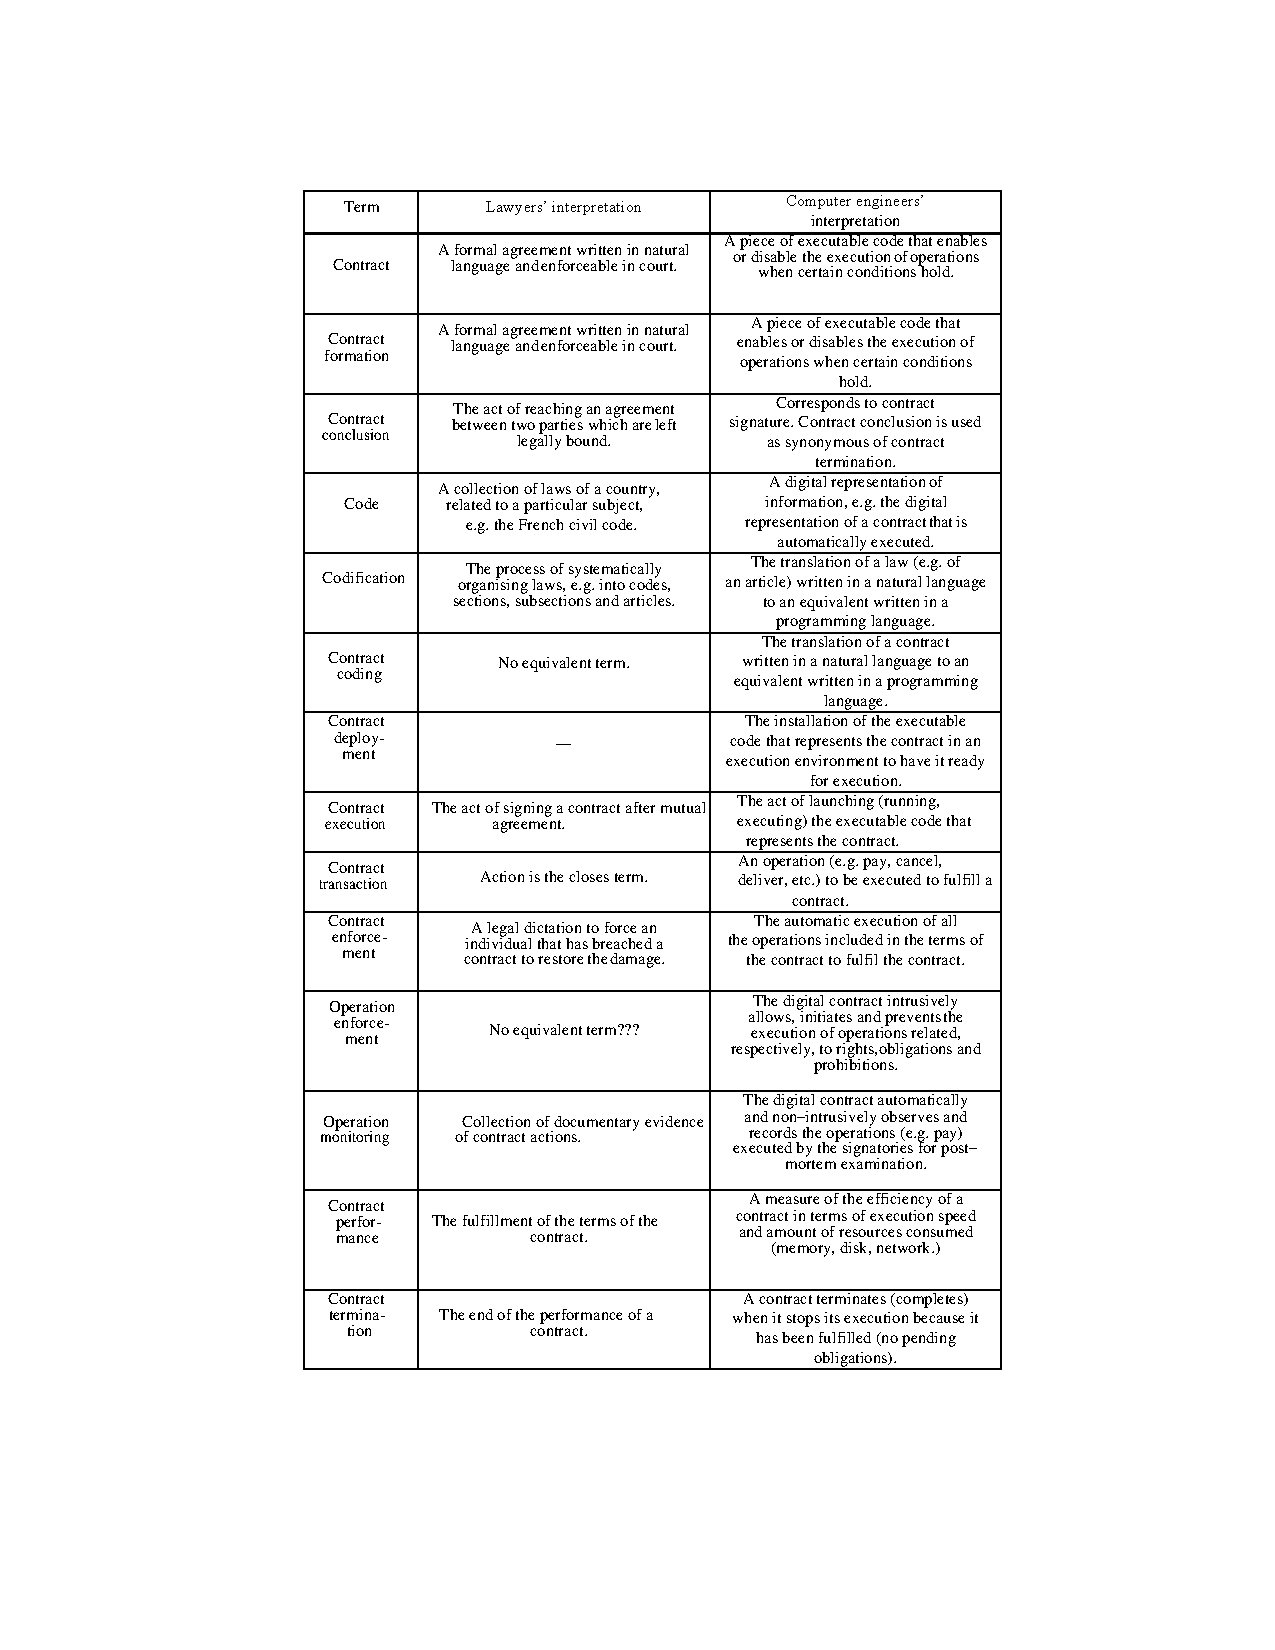
\includegraphics[width=0.85\columnwidth]{imagenes/terminosdiferentescontratos.pdf}
\caption{Comparison of contract terminologies.}
\label{terminosdiferentesontratos}
\end{figure} 


Esta figura \ref{vusftollsbrgitmsd.pdf}


\begin{figure}
\centering
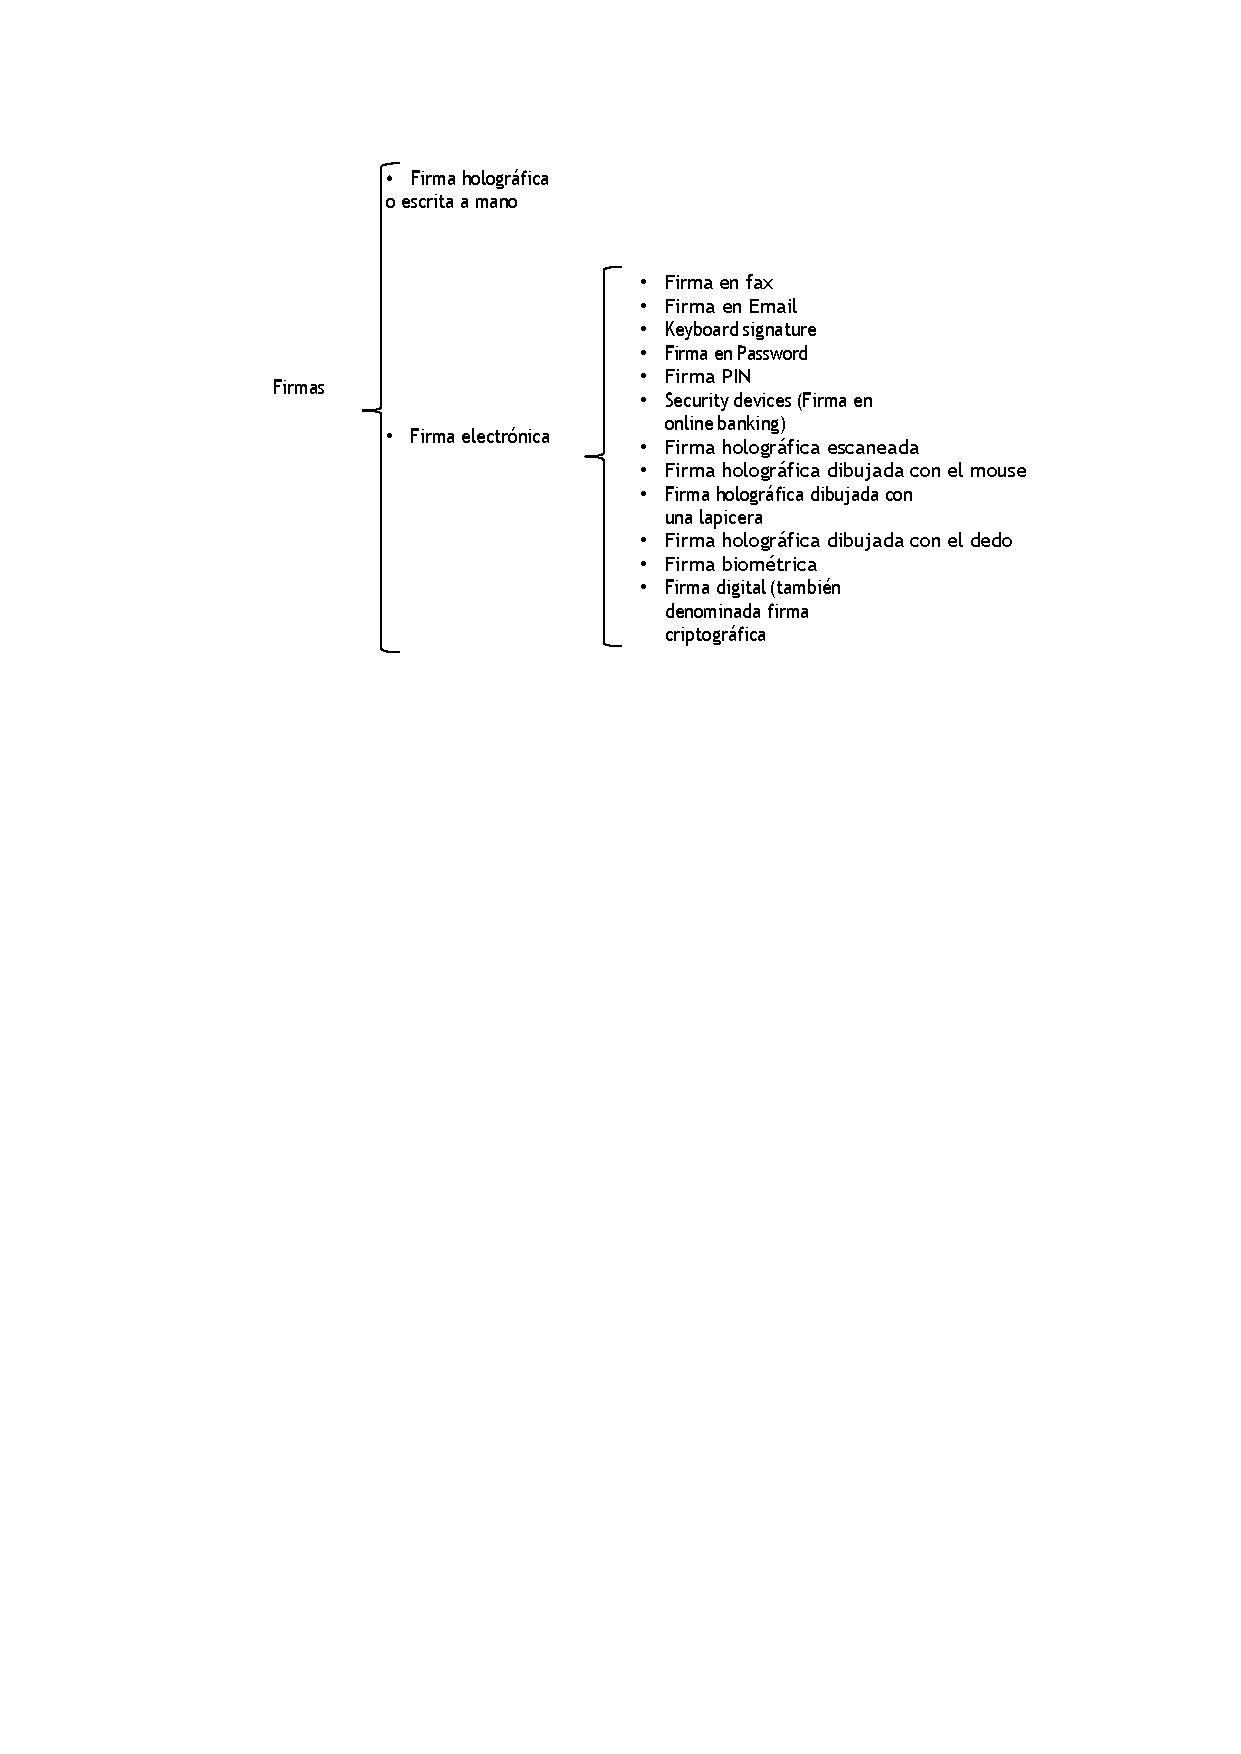
\includegraphics[width=0.85\columnwidth]{imagenes/cuadrollavefirmas.pdf}
\caption{Categorisation of signatures from the perspective of technology used to place them.}
\label{vusftollsbrgitmsd.pdf}
\end{figure} 

La tabla. 2 presentan un resumen de la terminología utilizada por los abogados e ingenieros informáticos.


\section{Firmas y contratos}

Actualmente se utilizan varios tipos de firmas en el comercio electrónico. Desde la perspectiva de la tecnología electrónica se pueden agrupar en dos categorías:

\begin{itemize}
    \item Firmas realizadas a mano u holográficas: también llamadas firmas manuscritas, son firmas plasmadas en papel con tinta química. No utilizan tecnología electrónica.
    
    \item Firmas electrónicas: son firmas realizadas a través de tecnologías electrónicas como fax, correo electrónico, números pin, botones de aceptación, clave pub-priv y otras tecnologías. \footnote{\cite{Andersson2020}Security Engineering: A Guide to Building Dependable Distributed Systems}

    \item Firmas basadas en clave pública: son las firmas electrónicas más sofisticadas. Por tal motivo, normalmente se tratan por separado bajo el nombre de firmas digitales o firmas criptográficas. En nuestro trabajo utilizaremos el término firmas electrónicas no digitales para referimos a cualquier firma electrónica con excepción de las firmas basadas en claves privadas.

    \end{itemize}

   La Fig. 12 muestra un resumen de las firmas que están actualmente en uso.


    \subsection{Contratos firmados manualmente y contratos firmados electrónicamente}

Con respecto al tipo de firma que se coloca en un contrato legal, distinguimos entre
dos clases de contratos:

\begin{itemize}
    \item Contratos firmados manualmente.

    \item Contratos firmados electrónicamente.
    
\end{itemize}

La Fig. 13 resume el punto. Los contratos firmados manualmente están protegidos por firmas efectuada de la manera convencional, es decir, una firma holográfica escrita con una pluma de tinta en una hoja de papel. Los contratos firmados electrónicamente llevan firmas colocadas usando una de las tecnologías que se muestran en la Fig.13. Algunos autores los llaman “contratos firmados en línea” para enfatizar que el acto de firmar se lleva a cabo en línea, en el sentido de que el documento firmado se transmite en línea a las partes interesadas. Usaremos ambos términos indistintamente en comentarios posteriores. Mostraremos ejemplos específicos en la Sección 4.

\section{ Contratos no automáticos }

La característica más destacada de los contratos no automáticos es que se \textit{cumplen o realizan} de forma manual, es decir, la ejecución de sus acciones no implica la ejecución del código informático. Resaltamos que, en relación con la ejecución o celebración del contrato, la firma es un tema diferente. De hecho, los contratos no automáticos (los objetos de interés de esta sección) se pueden firmar de forma manual o electrónica. Los discutiremos por separado. 

\subsection{Contratos firmados manualmente }


	Definimos a un contrato \textbf{firmado manualmente} como un contrato legal negociado, escrito exclusivamente en lenguaje humano en una hoja de papel, firmado por medio de firmas manuscritas y realizado o cumplido sin la asistencia de tecnología informática. Los contratos firmados manualmente son los contratos tradicionales que se han utilizado durante siglos. La Fig. 14 muestra un ejemplo de un contrato hipotético firmado manualmente escrito en español y acordado entre Alice y Bob (los firmantes). 

\subsubsection{Formato y firma del contrato }

Para firmar el contrato, Alice y Bob se reúnen en un lugar físico, imprimen dos copias del contrato (el documento que se muestra en la Fig. 14) en papel (A4 o papel carta) y las firman simultáneamente con un bolígrafo de tinta húmeda. Alice se queda con una copia y Bob con otra Los documentos firmados se almacenan en archivadores tradicionales.

\begin{figure}
\centering
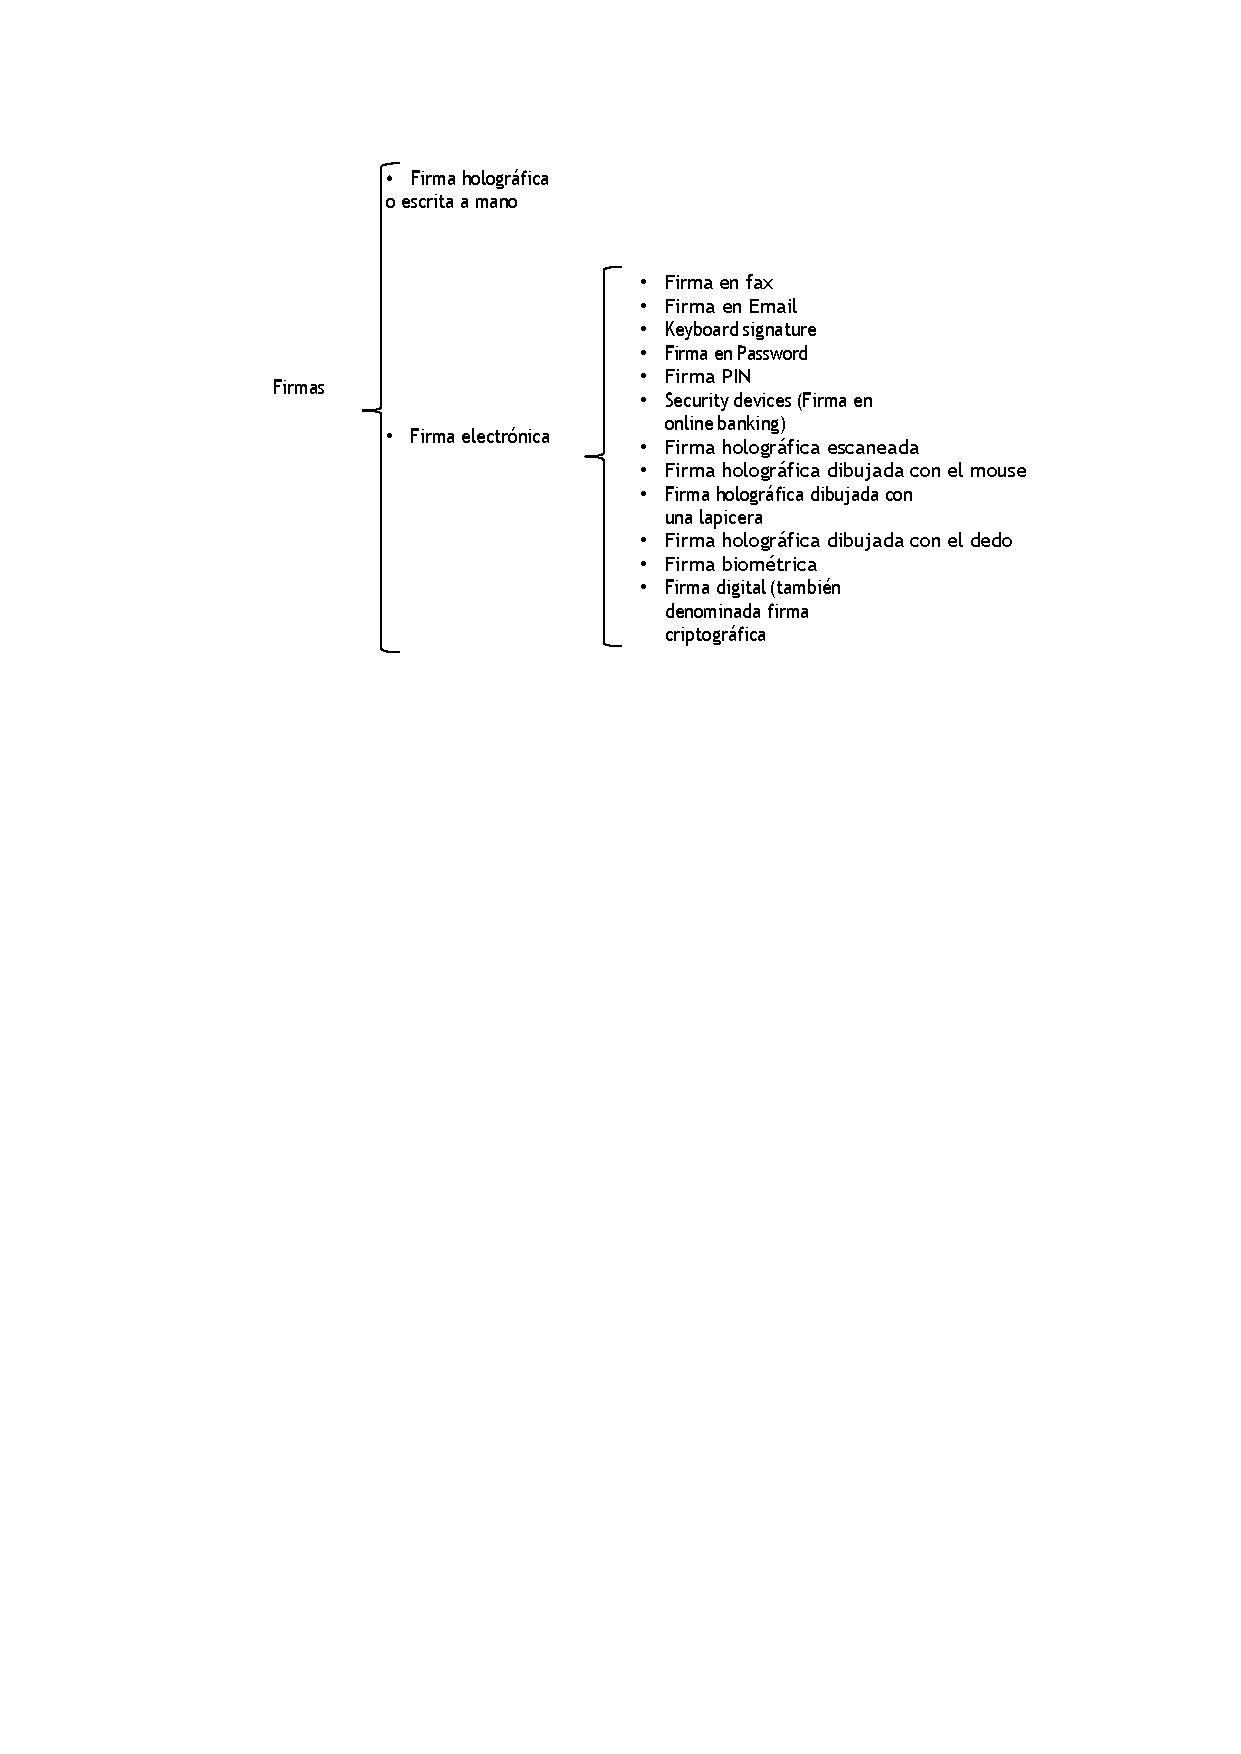
\includegraphics[width=0.85\columnwidth]{imagenes/cuadrollavefirmas.pdf}
\caption{Categorisation of signatures from the perspective of technology used to place them.}
\label{vusftollsbrgitmsd.pdf}
\end{figure} 


Esta figura \ref{ejcontfirmman.pdf}


\begin{figure}
\centering
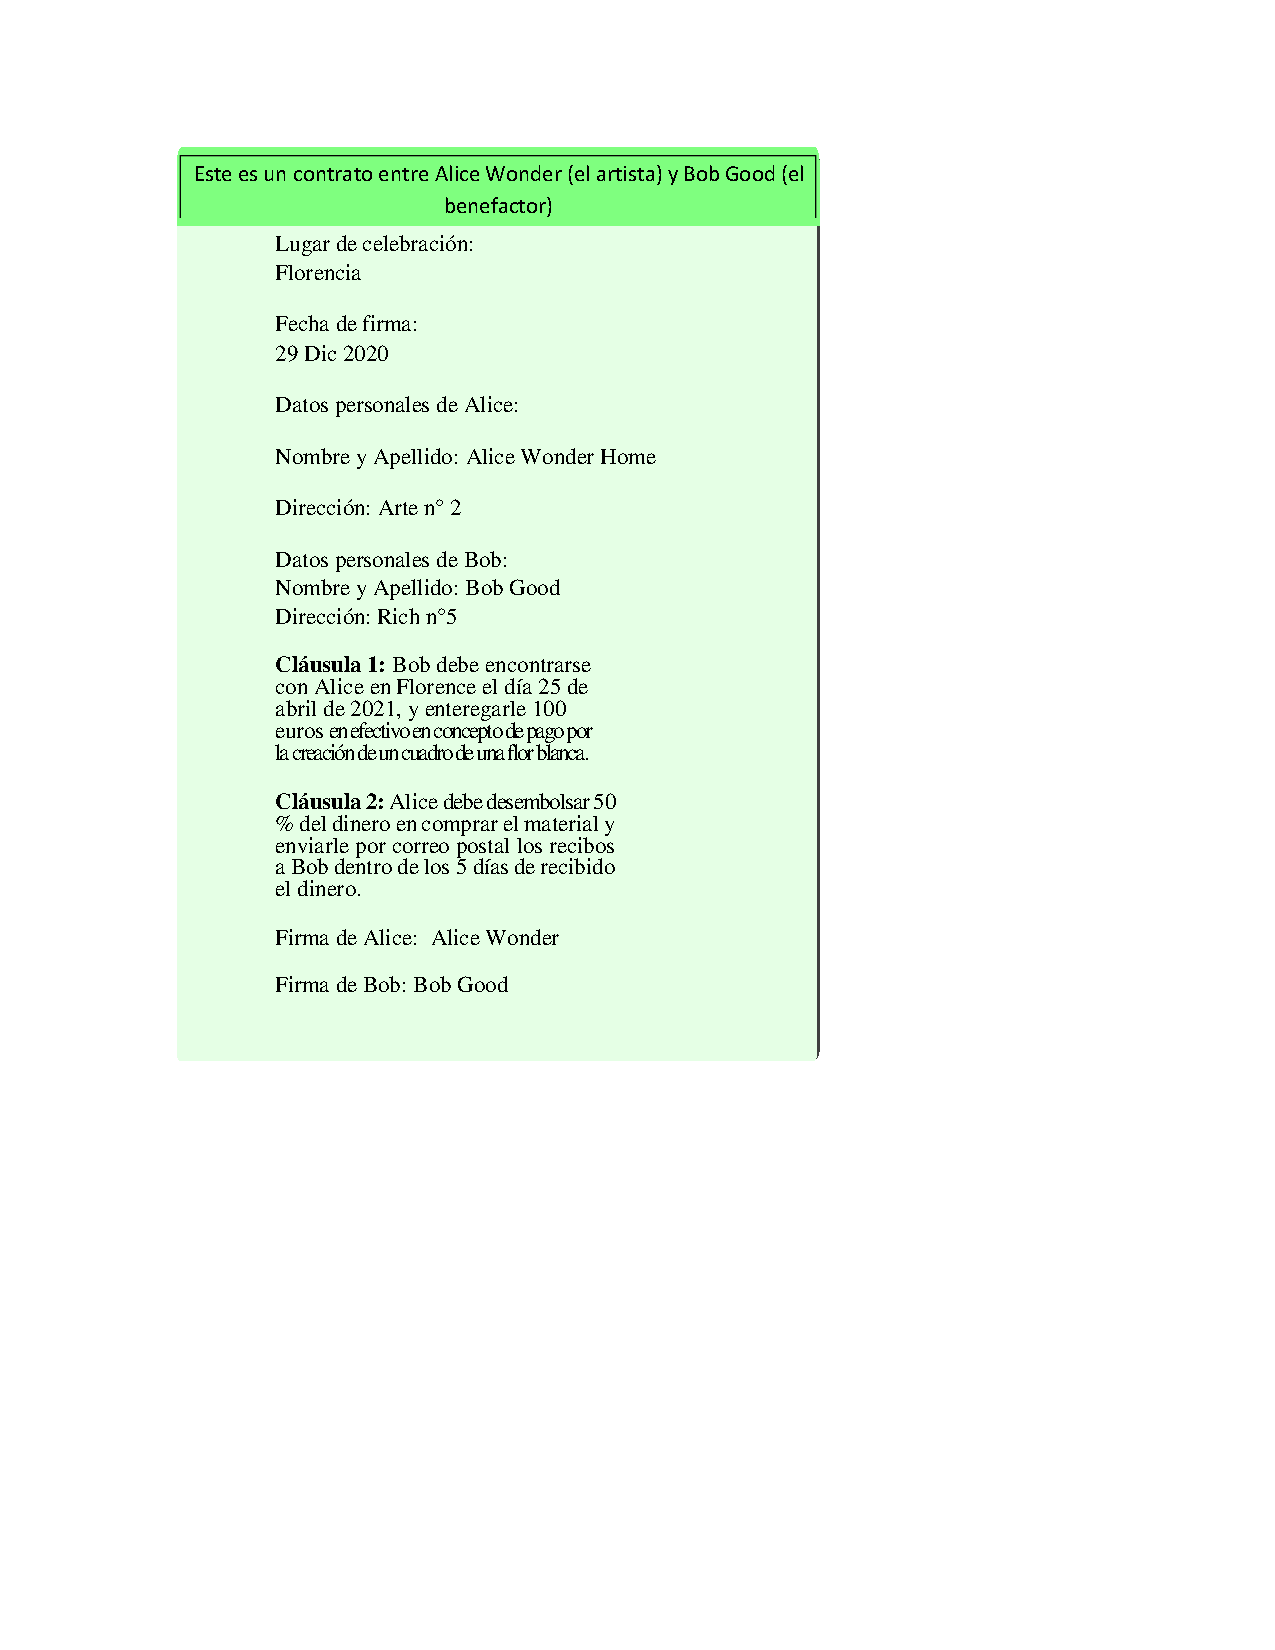
\includegraphics[width=0.85\columnwidth]{imagenes/ejcontfirmman.pdf}
\caption{falta nombre.}
\label{ejcontfirmman.pdf}
\end{figure} 

\subsubsection{Ejecución del contrato}

La Fig. 15 muestra la celebración o ejecución de un contrato firmado manualmente. Alice o Bob no tienen dispositivos informáticos. Decimos esto para enfatizar que no utilizan tecnología informática para celebrar o ejecutar el contrato. En efecto, dado que las operaciones especificadas en las cláusulas del contrato implican la manipulación de objetos físicos (efectivo y documentos en papel, respectivamente), este contrato no puede ejecutarse automáticamente. Es un contrato ejecutable de forma manual. En la figura, las flechas etiquetadas como interacción indican que Alice y Bob interactúan con la hoja de papel A4 firmada de la manera tradicional.

Aclaramos que puede haber ejemplos de contratos que incluyan operaciones que pueden ser automatizados; sin embargo, si Alice y Bob deciden realizarlo o celebrarlo o suscribirlo o ejecutarlos de manera tradicional y no convertirlo a código digital, entrarán en la categoría de contratos ejecutados manualmente.


\subsection{Contratos firmados electrónicamente}

Definimos a un contrato firmado electrónicamente como un contrato legal negociado y firmado por medio de una firma electrónica de clave pública y privada.

\subsubsection{Formato y firma del contrato}

La Fig. 16 muestra un ejemplo de un contrato hipotético firmado electrónicamente por Bob a través de un mensaje de correo electrónico enviado desde su dispositivo y firmado por Alice a través de una respuesta de correo electrónico enviada desde su dispositivo. Destacamos que los dispositivos son utilizados por Bob y Alice solo para firmar el contrato. El contrato se firma online, es decir a distancia, y, en consecuencia, no está firmada simultáneamente por Alice y Bob —uno de ellos siempre
lo firma primero.

\subsubsection{Ejecución del contrato}

La Fig. 17 muestra la ejecución del contrato. Suponemos que se realiza (ejecuta, en la jerga informática) sin ninguna tecnología, Se espera que Alice llame a la Oficina local de Western Union para cobrar en efectivo el pago de Bob. En otras palabras, la operación, "Pagar 100 a Alice" no se realiza automáticamente.

La pregunta que surge aquí es la validez de la firma de Bob. Obsérvese que Bob envía su correo electrónico desde una cuenta de gmail.com, por lo que Bob@gmail.com es una firma, alguien puede preguntarse, quién lo certifica. Es bien sabido que no es difícil abrir una cuenta de correo electrónico en gmail y otros servicios de correo electrónico gratuitos como Hotmail bajo datos personales falsos como nombre falso, edad, sexo, ubicación, etc. Desde la perspectiva de la confianza, la dirección de correo electrónico de Bob es diferente de Alice@cam.ac.uk, de Alice, que le fue otorgada por la Universidad de Cambridge, una institución de confianza.

COLOCAR Figure 16. An online signed contract written in English.

Creemos que esta pregunta necesita un análisis profundo; argumentamos que decir que los emails son aceptados como firmas electrónicas legales es engañoso; tal vez no todos son.

\section{Creemos que esta pregunta necesita un análisis profundo; argumentamos que decir que los emails son aceptados como firmas electrónicas legales es engañoso; tal vez no todos son.}


Los contratos se pueden clasificar en contratos tradicionales (sin automatización) y contratos digitales con diferentes grados de automatización. En esta sección, discutiremos cinco sub-clases de contratos digitales que existen en el espectro entre la ausencia de automatización y la automatización plena o total:

\begin{itemize}
    \item Contratos redactados en lenguaje natural.
    \item Contratos escritos únicamente en código.
    \item Contratos escritos en código, pero respaldados por un contrato tradicional.
    \item Contratos híbridos.
    \item Contratos multimedia.   
\end{itemize}

En \footnote{. C. et al., “Smart contracts: 12 use cases for business and beyond.” \url{http://digitalchamber.org/assets/ smart-contracts-12-use-cases-for-business-and-beyond.pdf}, Dec. 2016. Prepared by: Smart Contracts Alliance — In collaboration with Deloitte, Visited on 15 Jun 2021.}  distinguen cuatro tipos de contratos...

\subsection{contrato de lenguaje natural}

Definimos a un \textbf{contrato en lenguaje natural} como un contrato que i) está escrito en lenguaje natural (por ejemplo,español, inglés) en una hoja de papel (por ejemplo, A4) ii) firmado solo con firmas manuscritas y iii) incluye uno o más compromisos contractuales que son exigibles automáticamente por medio de un código de computadora ejecutable. En algunos contratos, todas las cláusulas se pueden ejecutar  automáticamente, pero en otras, solo algunas de ellas.


COLOCAR Figure 18. A natural language contract.

La Fig. 18 muestra un ejemplo de contrato en lenguaje natural que se puede ejecutar  parcialmente de manera automática. La cláusula 1 se refiere a la transferencia de dinero a través de operaciones bancarias, por consiguiente, se puede traducir a un código de computadora ejecutable y llevarse a cabo automáticamente. Sin embargo, la cláusula 2 implica la transferencia de elementos tangibles (recibos impresos en papel) por correo postal, por lo tanto, sólo puede realizarse de la manera tradicional. Por consiguiente, este contrato puede ser cumplirse en forma automática sólo parcialmente.

\subsubsection{Formato y firma del contrato}

La firma del contrato es la misma que en los contratos firmados manualmente (ver Sección 14); sin embargo, la ejecución o celebración o suscripción es diferente. Alice y Bob se encuentran en un lugar físico, imprimen dos copias del contrato (el documento que se muestra en la Fig. 18) en papel (A4 o papel de carta) y las firman simultáneamente. Alice se queda con una copia y Bob con otra. Las hojas A4 firmadas se almacenan en archivadores tradicionales, pero también se utilizan para la codificación de las cláusulas que se ejecutan automáticamente, cláusula 1 en el ejemplo de la Fig.18.

COLOCARFigure 19. Coding of clause 1 in executable computer code

\subsubsection{Codificación de contratos}

El código ejecutable que se utiliza para hacer cumplir la Cláusula 1 se implementa  de la siguiente manera:

\begin{enumerate}
    \item Alice y Bob acuerdan contratar a Peter (un programador profesional o ingeniero de software) para producir el código ejecutable que intentará cumplir la obligación de Bob expresada en la Cláusula 1, automáticamente. La codificación del contrato se muestra conceptualmente en la Fig. 19.
    \item Peter traduce el texto en inglés de la Cláusula 1 a un lenguaje de programación. A este nivel de discusión, el lenguaje específico es irrelevante, por ejemplo, puede usar un lenguaje de blockchain como el script de Bitcoin y Solidity de Ethereum o un lenguaje de programación de propósito general como C++ o Python. Usaremos este último para ilustrar la situación. El código que se muestra en la Lista 1 está lejos de ser una traducción precisa de la Cláusula 1. Su objetivo principal es dar una idea aproximada sobre cómo se ve una cláusula contractual cuando se traduce a código ejecutable.

    \item Peter produce el código fuente Clause1.py que se muestra en la Lista 1. Decimos que los códigos fuente como Clause1.py son ejecutables en el sentido de que pueden ser ejecutados por una computadora directamente si se presentan a un intérprete o después de compilarlos con la ayuda de un compilador.

   
\end{enumerate}

COLOCAR Listing 1 Pseudocode of clause 1 of contract shown in Fig. 18

\subsubsection{Ejecución del contrato}

La Clause1.py puede considerarse como un mecanismo (una herramienta de software o un agente) que ciegamente realiza la operación estipulada en la Cláusula 1. La Clause1.py es solo una parte de código de computadora sin noción de contratos. Por lo tanto, las disputas potenciales que podrían surgir de su ejecución se resolverám con la asistencia del documento firmado que figura en Fig. 18 después de recuperarlo de los archivadores.

Probablemente, antes de delegar la responsabilidad de cumplir con la ejecución de la Cláusula1, Alice y Bob verificarán minuciosamente que Clause1.py haga exactamente lo que estipula la cláusula 1. Comprobarán a fondo (posiblemente con la ayuda de los auditores) que Pedro tradujo correctamente la Cláusula 1 en Clause1.py. Igualmente importante, después de aceptar Clause1.py como válido, Alice, Bob y Peter recurrirán a mecanismos criptográficos (por ejemplo, hash, también llamados resúmenes) para garantizar que nadie pueda alterar la Clause1.py sin que Alice, Bob y Peter sean capaces de detectar la alteración.

COLOCAR Execution of a contract written in natural language.

Vale la pena enfatizar que, como se muestra en la Fig. 20, la ejecución de la Clause1.py tiene lugar en una sola computadora, es decir, el código se ejecuta de manera centralizada. La ejecución descentralizada de Clause1.py también es posible y una mejor alternativa en algunas aplicaciones Discutiremos este enfoque y los problemas que plantea en las siguientes secciones; por el momento, el enfoque centralizado que tomamos en la Fig. 20 es suficiente para explicar las ideas centrales sobre los contratos escritos en lenguajes naturales. También es importante tener en cuenta que el código no está directamente vinculado al documento que se muestra en la Fig. 18, en el sentido de que no existen mecanismos automáticos (por ejemplo, un enlace URL o una relación criptográfica) para relacionar Clause1.py con el texto de la cláusula 1 en la Fig. 18.

\subsection{Contrato escritos únicamente en còdigo}

Definimos un \textbf{contrato escritos ùnicamente en código} como un contrato cuyas cláusulas son expresadas únicamente en código ejecutable y no lleva firma manuscrita ni criptográfica.

La Fig. 21 muestra el ejemplo de un documento que se utiliza para producir el código de contrato que se muestra en la Lista 2. Obsérvese que en este ejemplo, tanto la Cláusula 1 como la Cláusula 2 son susceptibles de traducción a código ejecutable de computadora.

\subsubsection{Formato y firma del contrato}

Alice y Bob aceptan los compromisos estipulados en la cláusula 1 y la cláusula 2. Además, acuerdan confiar el uno en el otro; en consecuencia, no firman el documento. Esto es un solución sensata cuando Alice y Bob se conocen o cuando las dificultades de la firma manuscrita sopesan sobre los beneficios, por ejemplo, porque Alice y Bob se encuentran en diferentes países. Desde una perspectiva legal, siempre que los requisitos de formación de los contratos se cumplen; oferta, aceptación, \textit{consideration (common law)} e intención de crear relaciones jurídicas, entonces se ha formado un contrato.

COLOCAR Figure 21. Contract recorded solely in code.

\textbf{Almacenamiento del contrato:} No se utiliza ninguna versión en papel del contrato. La única representación del acuerdo es el código ejecutable que implementa la cláusula 1 y la cláusula 2.

\textbf{Codificación de contratos}

El contrato se ejecuta automáticamente, es decir, sin intervención humana ni acción. La ejecución automática solo es posible cuando, como en este ejemplo, todas las cláusulas incluidas en el acuerdo son susceptibles de traducción a código ejecutable.

Una limitación que podría no ser aceptable en algunas aplicaciones es que la ejecución del código no está vinculado a ningún contrato legal firmado por Alice y Bob. Esto significa que en el caso de disputa, Alice y Bob solo pueden recurrir al código ejecutable para remover? o a antecedentes probatorios para demostrar los compromisos y términos del contrato. No obstante, siempre que el código informático refleje los requisitos de formación del contrato, entonces se ha formado un contrato. Sin embargo, introduce una cuestión adicional, a saber, que el código de la computadora debe, en algún sentido, ser traducido para determinar el verdadero significado lingüístico. Esto es una deficiencia y no es tan efectivo como se cree, causando  dependencia en la información de antecedentes y en el acuerdo, como conversaciones, correos electrónicos y similares, en caso de que existan.


El código ejecutable para realizar la Cláusula 1 y la Cláusula 2: un programador profesional, por ejemplo, Pedro escribe el código ejecutable para cumplir la Cláusula 1 y la Cláusula 2. El proceso es similar al que se muestra en la Fig. ??, excepto que esta vez tiene que traducir en código tanto la Cláusula 1 como la Cláusula. Los resultados se muestran en la Lista 2.

COLOCAR Listing 2 Code of contract shown in Fig. 21

\subsubsection{Ejecución del contrato}

La Fig. 22 muestra la ejecución de un contrato escrito únicamente en código.

\subsection{Contrato escrito en papel y en código}

Definimos un \textbf{contrato escrito en papel y código} como un contrato con cláusulas que son expresadas en código ejecutable y vinculado criptográficamente a un contrato firmado a mano.

\subsubsection{Formato y firma del contrato}

\subsubsection{Codificación de contratos}

La motivación para vincular el código ejecutable de las cláusulas a un contrato firmado a mano. es abordar una limitación destacada de los contratos escritos únicamente en código. Una particularidad de estos últimos es que su código no  deriva de documentos firmados. Una mirada cercana en la Fig. 21 y la Fig. 22 revelará que ni el texto del contrato ni el código ejecutable  que implementa sus cláusulas (cláusula 1 y cláusula 2) están firmados.

COLOCAR Figure 22. Execution of a contract written solely in code.

Esta particularidad puede ser inaceptable en algunas aplicaciones ya que el contrato escrito únicamente en código podría no satisfacer los requisitos de la jurisdicción donde se ejecuta el código. Una posible solución a este problema es vincular criptográficamente el texto firmado del contrato a su código ejecutable, de la siguiente forma: Alice y Bob firman a mano el texto del contrato como se muestra en la Fig. 23. A continuación, el programador (por ejemplo, Peter) puede escanear el papel firmado para producir un documento digital (por ejemplo, en formato jpeg o pdf); llamémoslo firmadoContrText.jpeg. Luego, Pedro puede hacer hash firmedTextContr.jpeg para producir un hash (también llamado huella digital) de
firmadoTextContr.jpeg, por ejemplo, QmSNZBkCaRsAnDrAX3JgYsHm4n2aZmoRbSo. El hash garantiza que el texto del contrato no puede ser alterado. También puede ser utilizado como una dirección para almacenar el documento firmadoTextContr.jpeg en un sistema de archivos, por ejemplo en el IPFS. Igualmente importante, el hash se puede codificar en el código ejecutable que ejecuta las cláusulas del contrato de manera que el código y el archivo firmadoTextContr.jpeg están vinculados criptográficamente entre sí. Otra medida de seguridad que Alice y Bob pueden tomar es codificar el código ejecutable después de codificar el hash QmSNZBkCaRsAnDrAX3JgYsHm4n2aZmolUoR para garantizar que el código no pueda ser modificado. La idea se muestra en la Lista 3 donde la línea 30 (en azul) incluye el hash de firmadoTextContr.jpeg.

COLOCAR Listing 3 CClause1.py implements clause 1 and 2 of contract of Fig. 23

Figure 23. Contract recorded on paper and code.

Figure 24. Execution of a contract written on paper and code (see Fig. 23).

\subsubsection{Ejecución del contrato}

La Fig. 24 muestra la ejecución del código de la Lista 3. Nótese que el código de la cláusula 1 está vinculado al archivo firmadoTextContr.jpeg que Peter produjo después de escanear el documento que se muestra en la Fig. 23

\subsection{Contratos híbridos}

Un contrato híbrido es un contrato que se ejecuta y se hace cumplir mediante un código ejecutable informático en colaboración con humanos. Es decir, existe parte en  código de computadora y parte en texto lingüístico, y su ejecución ocurre parcialmente en la automatización de la computadora y en la intervención humana.

Concretamente, definimos a un contrato híbrido como un contrato que reúne dos condiciones:

\begin{itemize}
    \item El contrato se escribe en código que puede ser recuperado por un programa lector desde un archivo, interpretado y desplegado en una pantalla de computadora como texto legible para humanos
    \item El contrato se firma bajo firmas criptográficas.
        
\end{itemize}

Normalmente, un contrato híbrido incluye uno o más compromisos contractuales expresados como código ejecutable que se puede ejecutar para automatizar total o parcialmente su ejecución o celebración  y su exigibilidad o cumplimiento. Por total y parcialmente automático queremos decir que el código ejecutable se puede programar para que se ejecute hasta el final sin intervención humana o para ejecutar en modo conversacional. En este modo, el código ejecutable puede detenerse varias veces durante su ejecución para solicitar la intervención (digamos algunos datos de entrada o instrucciones de qué hacer a continuación) de los humanos cuando se necesita el juicio humano.

El elemento central de los contratos híbridos es el límite criptográfico entre el código ejecutable y el documento que contiene el texto legible por humanos. Nótese que algunos autores se refieren a los contratos híbridos como \textbf{contratos ricardianos}. \footnote{\cite{IanGrigg2015} On the intersection of ricardian and smart contracts}

Elaboramos estos puntos con la ayuda del ejemplo que se muestra en la Fig. 25.

COLOCAR Figure 25. Contract to be translated into a hybrid contract.

\subsubsection{sectionFormato y firma del contrato}

Una limitación destacada de la ejecución de los contratos en lenguaje natural que se muestra en la Fig. 18, es la separación física y lógica entre el contrato y el código que implementa la cláusula 1 (ver ejecución en Fig. 20) La conexión entre el contrato en lenguaje natural que se muestra en la Fig. 18 y el código de la Lista 1, se hace manualmente en el sentido de que Alice y Bob no cuentan con mecanismos automáticos para relacionar el código de la Lista 1 al texto de la Fig. 18. Por ejemplo, no tienen mecanismos para navegar (i.e., por medio de clics del mouse) del texto de la Fig. 18 al código ejecutable en ejecución que se muestra en la Fig. 20 o al revés, desde el código ejecutable de la Fig. 20 hasta el texto que se muestra en la Fig. 18. Este inconveniente se agudiza en el contrato escrito únicamente en código, como el ejemplo de la Fig. 21. Obsérvese que las ejecuciones de la Cláusula 1 y la Cláusula 2 que se muestran en la Fig. 22 no son respaldadas por un contrato legal, no hay ningún texto que Alice, Bob o alguien más (por ejemplo, un juez) puedan referirse para evaluar la ejecución que tiene lugar en la figura. Estas limitaciones se pueden abordar con la ayuda de contratos híbridos de las cuales se muestra un ejemplo en la Fig. 25.

\subsubsection{Codificación de contratos}

Supongamos que Alice y Bob contratan a Peter (un programador profesional) y delegan en él la responsabilidad de producir un contrato híbrido correspondiente al texto que se muestra en la Fig. 25. El programador produce la Lista 4, que es el texto que se muestra en la Fig. 25 pero complementado con etiquetas y las claves públicas de los participantes, de Alice y Bob respectivamente. Para simplificar la explicación, en este ejemplo asumimos que Peter usa notación JSON, pero se pueden usar otros lenguajes de etiquetas, incluido XML.

COLOCAR Listing 4 ...

Como se muestra en la Lista 4, asumimos que Alice y Bob acordaron que la cláusula 1 debe ser ejecutada automáticamente y la cláusula 2 manualmente. En consecuencia, Alice y Bob delegan la responsabilidad de traducir la cláusula 1 al código ejecutable. El proceso es el mismo que la conversión de la cláusula 1 del contrato en lenguaje natural que se muestra en la Fig. ?? excepto que Peter produce un contrato firmado digitalmente.

Hacemos la misma suposición con respecto a la corrección de la conversión, es decirr, Alice y Bob necesitan verificar que el código producido por Peter corresponda a lo que está estipulado en el texto de la cláusula 1. Probablemente, probarán el código de Peter cuidadosamente antes de proceder a firmar el contrato bajo sus firmas criptográficas. Supongamos que la verificación del código es exitosa y que Alice y Bob firman criptográficamente el contrato híbrido. El resultado se muestra en la Lista 5. Se pueden ver las firmas de Alice y Bob en las últimas líneas del texto.

COLOCAR Listing 5 Code signed by Alice and Bob to produce a hybrid contract.


Una de las fortalezas de los contratos híbridos se muestra en las claves de las cláusulas, es decir, ”implementación” y code\_hash\_and\_addr. La clave “implementación” de la cláusula 1 indica que la clausula 1 debe ejecutarse automáticamente, en este ejemplo, con la ayuda del código producido por Peter a partir del texto de la cláusula 1. El valor (QmSNZBD-kCa3...Hm4n2aZmolVUoR) de la clave code\_hash\_and\_addr es el hash del código producido por Pedro. Se utiliza con tres propósitos: es una huella digital que garantiza la integridad del código: no se puede alterar sin ser detectado; el hash también se utiliza como un identificador único del código y también, como la dirección para guardar el código en un sistema de archivos Si Alice y Bob almacenaran el código en el sistema de archivos IPFS, estaría bajo la dirección QmSNZBDkCa3...Hm4n2aZmolVUoR. Como se muestra en la Fig. 27, el hash se utiliza para vincular el código al contrato híbrido.


COLOCAR Figure 26. Coding of a hybrid contract.

La clave de "implementación" muestra que la cláusula 2 debe ejecutarse manualmente, respectivamente, el valor de code\_hash\_and\_addr es "NIL". La Fig. 26 muestra un resumen de los procedimientos para producir el contrato híbrido firmado con la ayuda de Peter.

\subsubsection{Ejecución del contrato}

Una característica destacada de un contrato híbrido es que puede ser leído tanto por humanos como por programas de computadoras:

\begin{itemize}
    \item Legible por humanos: significa que un humano como Alice y Bob puede mirar el texto (ver Lista 4) y entender lo que el documento estipula y sobre esta base, firmarlo criptográficamente para producir el documento que se muestra en la Lista 5. Asimismo, si la Lista 5 se presenta a un juez (por ejemplo, para resolver una disputa), él o ella podrán examinar el contenido del documento que en realidad es un contrato legal firmado.
    \item Legible por programa de computadora: significa que un programa de computadora es capaz de analizar o procesar e interpretar las etiquetas incluidas en el texto. Además, se puede utilizar para construir varios mecanismos para interactuar con el contrato híbrido. 

    
\end{itemize}

Por ejemplo, para ahorrarse la molestia de mirar las etiquetas incluidas en el texto, Alice puede usar un programa lector (también llamado visualizador o visor) que es capaz de interpretar las etiquetas y presentar un texto sin formato, limpio en la pantalla de la computadora. Como analogía, podemos mencionar que los lectores están incluidos en los navegadores convencionales (por ejemplo, Internet Explorer y Fire Fox) para mostrar páginas web que también son documentos etiquetados. Un buen lector podrá visualizar todo el documento en la pantalla o solo el componente solicitado por Alice o Bob, como el nombre completo del artista, el domicilio del benefactor o las cláusulas del contrato. Un lector más sofisticado incluirá funciones para ayudar a Alice y Bob a interactuar con el código ejecutable del contrato (con CClause 1 en este ejemplo); por ejemplo, para permitir que Alice solicite el estado actual de la ejecución, como qué cláusulas están pendientes, cuáles se han cumplido o violado, etc.  El lector también se puede instrumentar para verificar que el código ejecutable de CCaluse 1 no ha sido alterado. Un lector utilizado para interactuar con un contrato más complejo (ver el contrato multimedia en la Lista 6), que incluye varios componentes, pueden ser instrumentados para localizarlos y recuperarlos.

COLOCAR Figure 27. Execution of the hybrid contract

Obsérvese que en la Fig. 27, el contrato híbrido y el código ejecutable que implementa la cláusula 1 se refieren entre sí criptográficamente. En la figura, están colocados en la misma computadora, sin embargo, no hay dificultades técnicas para implementarlos en diferentes computadoras conectadas remotamente a través de Internet. Asimismo, vale la pena notar que la cláusula 2 también se puede considerar como la cláusula 1: se puede convertir en código y ejecutar automáticamente. y no necesariamente en la misma computadora que el código de la cláusula 1; la ubicación de los códigos que implementan las cláusulas es irrelevante siempre que se puedan alcanzar o comunicar. En general, un acuerdo se puede convertir en un contrato híbrido en su totalidad (todas las cláusulas) o parcialmente (sólo algunas de las cláusulas); todo dependiendo de la naturaleza de las cláusulas; algunas podrían tener una ambigüedad accidental o intencional que hace que no sea susceptible de codificación informática; se pueden codificar otras cláusulas, pero los participantes pueden decidir ejecutarlas manualmente, digamos, por razones de eficiencia o para mantener la flexibilidad que el juicio del hombre provee; otras cláusulas podrían implementarse de forma semiautomática, que es, implementado de manera que en alguna situación se ejecutará completamente hasta su finalización sin requerir intervención humana pero en otras situaciones se detendrá su ejecución y se enviará una señal de alarma (por ejemplo, un mensaje de correo electrónico) a los participantes para solicitar la intervención humana para proceder al siguiente paso de la ejecución.

\subsection{Contratos multimedia}

Vale la pena observar que el código de CClause1.py en la Fig. 27 puede considerarse como un objeto que contribuye a la composición del contrato híbrido. En este ejemplo, es un fragmento de código ejecutable, pero en general, puede ser cualquier información digital, incluyendo, texto sin formato, figuras, videos, música, etc. Esta generalización convertiría el contrato híbrido que se muestra en la figura en un contrato multimedia.

\subsection{Formato y firma del contrato}

Intuitivamente, definimos a un \textbf{contrato multimedia} como un contrato que se compone de varios elementos (objetos o piezas) de diferentes formatos como texto, código ejecutable, imágenes, sonido, video, etc.

De forma más precisa, podemos decir que un contrato multimedia debe cumplir las siguientes condiciones

\begin{itemize}
    \item El contrato tiene un componente principal que se escribe en código que se puede recuperar por un programa de lectura de un archivo, interpretado y desplegado en una pantalla de computadora como texto que sea legible para los humanos.

    \item Además del componente principal, el contrato incluye uno o más componentes multimedia  ubicados arbitrariamente en la web pero relacionados entre sí por medio de enlaces criptográficos.

    \item El contrato se firma bajo firmas criptográficas
\end{itemize}

La ejecución de un contrato multimedia es similar a la ejecución de un contrato híbrido, en el sentido de que se trata de un código ejecutable que cumple los compromisos contractuales de manera automática o semiautomática (cuando requieran intervención humana)  y cláusulas que se ejecutan únicamente de la manera tradicional. Usaremos Lista ?? para elaborar nuestro argumentos

Las ventajas de los contratos multimedia son numerosas. Creemos que pueden contribuir significativamente a la automatización de la ley: una ley donde la mayoría de las reglas se ejecutan automáticamente por contratos multimedia que se refieren a objetos multimedia, incluidos otros contratos.

\subsubsection{Codificación de contratos}
La lista 6 es un ejemplo de un contrato multimedia que incluye, además de las cláusulas contractuales del ejemplo anterior, dos componentes adicionales: el boceto de la pieza de arte que el artista se compromete a pintar y la foto de un trabajo similar del artista.

COLOCAR Listing 6 Multimedia contracts signed by Alice and Bob.

Figure 28. Execution of a multimedia contract.

\subsubsection{Ejecución del contrato}

La Fig. 28 muestra la ejecución del contrato multimedia que se muestra en la Lista 6. Nótese que este contrato multimedia está relacionado con tres componentes (objetos): el código de la cláusula 1 y dos elementos de arte, es decir, un boceto de la obra de arte que el artista se compromete a producir y una foto de un trabajo similar del artista. El contrato multimedia hace referencia a las piezas de arte a través de sus hashes. Los hashes se utilizan para identificar piezas de arte y como direcciones para ubicarlos en los sistemas de archivos donde están almacenados. De esta manera QmSkeBD-
kCa3...mHn2aZjimSMFiP y QmPhoQBkCa3...mHn2aZjimCMJab identifican de forma única el boceto y la foto, respectivamente. Destacamos que el contrato multimedia y todos sus componentes están ubicados en la misma computadora por conveniencia de esta presentación; en la práctica, es más probable que estén ubicados en una computadora diferente. Para simplificar, el contrato multimedia y sus componentes se muestran de forma aislada, en la práctica, es más probable que forme parte de un gráfico arbitrario de otros contratos y componentes similares, al igual que las páginas web  convencionales de Internet.

COLOCAR Figure 29. Execution of the multimedia contract with machine readable legislations.

Las legislaciones legibles por máquina se analizan en \footnote{\cite{Eva2020}“Regulatory technology: Replacing law with computer
code,”}

\section{Categorización adicional de contratos}

Esta sección resume el tema de la categorización de contratos y analiza tres
Categorías adicionales.

\subsection{Despliegue centralizado y descentralizado de contratos}

Desde la perspectiva de la infraestructura utilizada para su implementación, clasificamos contratos digitales en. Ver la figura 30.

\begin{itemize}
    
    \item Contratos digitales centralizados.

    \item Contratos digitales descentralizados

   
\end{itemize}

Decimos que un contrato digital está centralizado si solo se ejecuta (instanciado o ejecutado) una sola réplica (copia). En cambio, decimos que un contrato digital está descentralizado si dos o más réplicas se ejecutan. Usaremos la Fig.31 para explicar los principales problemas involucrados en una u otra alternativa. Observe que en la figura, usamos el término contrato inteligente (SC) en lugar de "contrato digital" para que coincida con el término utilizado por la comunidad blockchain.

COLOCAR Figure 30. Contract categories from the perspective of decentralisation.

Figure 31. Centralised and decentralised deployment of digital contracts.

Como se muestra en la figura, la única réplica de un contrato centralizado se implementa en una computadora (PC) administrada por un tercero de confianza (TTP) ubicado en Internet, por ejemplo, puede ser un proveedor de nube. Desde el punto de vista técnico, la ubicación física de la computadora es irrelevante, siempre y cuando sea accesible para Alice y Bob. La figura muestra un contrato digital descentralizado que ha sido replicado cuatro veces. Se ejecuta la réplica SC1 en P C1, la réplica SC2 se ejecuta en P C2 y así sucesivamente. P C1, P C2, P C3 y P C4 son computadoras conectadas a Internet y miembros (nodo) de una cadena de bloques. Ejemplos de cadenas de bloques
son Bitcoin, Ethereum e Hyperledger. El protocolo de sincronización que ejecuta las cuatro réplicas es un algoritmo de consenso. Las réplicas deben ejecutarse juntas para sincronizar sus estados. Por ejemplo, si SC2 cumplió y registró la ejecución de una operación de pago, tiene que difundir la información a SC1, SC3 y SC4 para garantizar que todas las réplicas registran el cumplimiento de la obligación de pago.

Como se explica ampliamente en el Capítulo Descentralización, la infraestructura blockchain que alberga el contrato digital ofrece varias ventajas y abre la puerta a una gran clase de aplicaciones de contratos. Desafortunadamente, plantea varias cuestiones legales que actualmente son escasamente comprendidas.

\subsection{Contratos bilaterales y multilaterales}

Desde la perspectiva del número de firmantes, los contratos se pueden clasificar en bilaterales cuando involucran solo a dos partes, y multilaterales cuando están firmados por más de dos partes Ver

Por otra parte, la definición de contrato comprendida en el artículo 1101 del Código Civil Francés [24] establece explícitamente que un contrato puede celebrarse entre dos o más personas. Los contratos multilaterales tradicionales no automáticos se utilizan en algunas aplicaciones como acuerdos multinacionales. Un ejemplo práctico de un contrato multilateral es un fianza que involucra a tres partes: una fiador (un proveedor de seguros), un obligante (la parte asegurada) y un principal (una parte que promete un servicio al obligante) . VER FIADOR, ETC. La doctrina jurídica ha  estudiado la versión automática de los contratos multilaterales (ver ejemplo ) pero son difíciles de entender. En algunas situaciones es posible dividir un contrato multilateral en un conjunto de varios contratos bilaterales y utilizar mecanismos para gestionar sus interdependencias. Dado que los contratos bilaterales se utilizan con mayor frecuencia y son más fáciles de comprender, en nuestro trabajo nos centraremos sólo en ellos.

\subsection{Trabajo futuro y discusión}

\subsection{¿Por qué los llamamos contratos digitales?}

Se puede argumentar que el término contrato digital...

Preferimos este término en lugar de contrato inteligente porque no encontramos este último intuitivo. De hecho, encontramos la palabra "inteligente" engañosa porque solo estamos hablando de código de computadora ejecutable sin noción de inteligencia. Algunos autores utilizan el término contrato electrónico; tenernos reservas al respecto porque en informática y otros campos relacionados, la palabra "electrónico" se utiliza para referirse a la tecnología de hardware (por ejemplo, circuitos y cables) que respalda la ejecución de contratos y otras aplicaciones de software. Consideramos a un contrato como un concepto de software que es independiente de la electrónica de la computadora; por lo tanto, preferimos no asociar el término electrónico con ellos.

Estamos de acuerdo en que "contrato ejecutable", "contrato automático", "contrato programable" y "contratos computacionales" son más intuitivos que los "contratos digitales". Sobretodo creemos que los dos últimos términos captan la idea con mayor precisión porque estamos hablando de contratos que se pueden programar en un lenguaje de programación para automatizar la ejecución de los compromisos contractuales. Habiendo aclarado este punto, todavía decidimos utilizar el término contrato digital para apoyar el término que actualmente es el más utilizado.

\subsection{Legalidad de los contratos digitales}

\subsection{Ejecución automática de acuerdos}

Definimos un acuerdo como...

La Fig. 33 muestra el ejemplo de un documento que estipula un acuerdo entre Alice y Bob sobre una donación. Nótese que el contrato incluye dos cláusulas (Cláusula 1 y la Cláusula 2) que son susceptibles de traducción a código ejecutable por computadora y que Alice y Bob acuerdan ejecutarlo automáticamente.

Por cierto, este es un ejemplo típico de un acuerdo establecido entre benefactores y artistas donde los primeros apoyan la creación de una obra de arte. Estos acuerdos se realizan con frecuencia en plataformas de crowdfunding y se ejecutan automáticamente en línea.

F\textbf{ormato y firma del acuerdo:} No se firma ninguna versión en papel del acuerdo bajo firmas holográficas. La única representación del acuerdo es el código ejecutable que implementa la cláusula 1 y la cláusula 2.

Esta es una solución sensata cuando Alice y Bob se conocen y confían el uno en el otro o cuando las dificultades de firmar a mano el documento sobrepasan los beneficios. Por ejemplo, Alice y Bob se encuentran en diferentes países. También sería poco práctico para Alice firmar a mano el acuerdo con Bob si su donación es pequeña y Alice recibe cientos de ellos de diferentes benefactores.

Sin embargo, desde una perspectiva legal, este acuerdo no puede ser considerado como un contrato legal en el \textbf{Common Law} porque no cumple con todos los requisitos. Precisamente, no incluye una etapa de oferta que comprometa a Bob en un contrato legal. Por lo tanto, la ejecución que se muestra en la Fig. 34 es la ejecución automática de un acuerdo. Este ejemplo muestra que los contratos inteligentes tal como se conciben en Ethereum y otras cadenas de bloques no constiutyen necesariamente contratos legales

\textbf{Ejecución del contrato:} El contrato se ejecuta automáticamente, es decir, sin intervención o acción humana (ver Fig. 34). Esto es posible porque todas las cláusulas incluidas en el acuerdo son susceptibles de traducción a código ejecutable.

\subsubsection{Resumen}

La Fig. 35 presenta un resumen de la categorización de contratos desde la perspectiva de la automatización y sus principales características.

	La tabla 3 resume...
 
	La Tabla 4 presenta un resumen de las principales características que distinguen a los

\subsection{Ley Computacional}

Uno de los usos más ambiciosos y prometedores de los contratos digitales es   la automatización de la ley. Es un concepto emergente recientemente al que se hace referencia con diferentes términos. En\footnote{\cite{PrimaveraAaron2018}Blockchain and the Law: The Rule of Code}  se llama Lex Cryptographia, en \footnote{Law.MIT.edu, “Computational law.”\url{ https://law.mit.edu}, 2021. Visited on 5 Jul 2021. [46] C. Law, “Nathaniel love and michael genesereth,” in Proc. 10th Int’l Conf. on Artificial Intelligence and Law, 2005. [47] M. Genesereth, “What is computational law?.” \url{https://law.stanford.edu/ 2021/03/10/what-is-computational-law/}, Mar. 2021. Stanford University.} se llama Ley Computacional, en \footnote{\cite{Eva2020}“Regulatory technology: Replacing law with computer code” } se denomina Sustitución de la Ley por Código Informático, en \footnote{\cite{Harry2012}“Computable contracts,” } se denomina Contratos Computables. También puede llamarse “ley programable”. La idea general detrás de todos estos conceptos es aprovechar los avances recientes en la tecnología informática para automatizar el cumplimiento de la normativa en diferentes campos de nuestra sociedad que van desde la regulación dentro de empresas privadas a los gobiernos. La implementación del código como ley resultaría en sociedades bajo gobierno algorítmico. Esto requerirá que la ley (código civil, códigos que incluyen derecho corporativo, derecho administrativo, derecho tributario, derecho constitucional, etc.) escrito en lenguaje natural para la interpretación humana se traduzca a un lenguaje que las computadoras puedan leer, interpretar y ejecutar automáticamente. El desafío parece más fácil en un sistema codificado de Derecho como el Derecho Civil o Romanista que en el sistema de Derecho Consuetudinario donde no existe una constitución escrita. Cómo la presencia o ausencia de una ley codificada impacta en la implementación del código como ley es una pregunta abierta. Por cierto, el texto en lenguaje natural de los contratos en el Derecho Civil (véase, por ejemplo, el Código Civil francés\footnote{\cite{JohnCart2016}, “French civil code 2016.” } ) es normalmente más corto que en el derecho consuetudinario porque el contrato puede simplemente referirse a reglas codificadas en lugar de incorporarlas explícitamente .\footnote{World Bank, “Key features of common law or civil law systems.” \url{https://ppp. worldbank.org/public-private-partnership/legislation-regulation/ framework-assessment/legal-systems/common-vs-civil-law}, 2020. Visited on 8 Aug 2021.} Si sus equivalentes digitales son más cortos, más fáciles de codificar y depurar (ver Fig. 5) es una pregunta abierta. Un interrogante que se ha planteado sobre los contratos automáticos es su falta de flexibilidad en comparación con los contratos tradicionales .\footnote{\cite{JeremySkla2018}“Smart contracts and the cost of inflflexibility} Esto significa que su uso en la implementación de la ley nacional comprometería la flexibilidad de la ley actual que se basa en la intervención de humanos para proporcionar juicio humano. Una posible solución a este problema es el uso de contratos híbridos como se muestra en la Sección 5.4 donde un humano interviene cuando se necesita el juicio humano. Si es necesario, se puede agregar más flexibilidad en este punto, por ejemplo, la decisión puede ser tomada por consenso, digamos por un grupo de personas. Además, se puede usar el seguimiento o monitoreo, en lugar de la exigibilidad o aplicación (como se discutió en la Sección 2.2.3).
... especular sobre IA, IoT, etc.

COLOCAR Figure 33. Donation agreement between Alice and Bob.

Figure 34. Execution of an agreement written solely in code.

\section{Trabajo relacionado }

El objetivo general de nuestro trabajo es ayudar a comprender la relación entre contratos legales tal como los conciben tradicionalmente los abogados y los contratos digitales tal como los conciben los ingenieros de software. Los primeros intentos de aclarar esta pregunta se han planteados antes por la doctrina \footnote{\cite{Christopher2019}“Smart contract templates: legal semantics and code validation.” \url{http://www0.cs.ucl.ac.uk/staff/C.Clack/research/ JDigitalBanking-Clack-AuthorPreprint.pdf}, 2019. Visited on 5 Dec 2020. C. D. Clack and C. McGonagle, “Smart derivatives contracts: the isda master agreement and the automation of payments and deliveries.” \url{https://arxiv.org/ pdf/1904.01461.pdf}, Apr. 2019. arXiv:1904.01461 [cs.CY]. [51] C. D. Clack, V. A. Bakshi, and L. Braine, “Smart contract templates: foundations, design landscape and research directions.” \url{https://arxiv.org/pdf/1608.00771. pdf}, Aug. 2016. arXiv:1608.00771 [cs.CY]. [52] S. D. Levi and A. B. Lipton, “An introduction to smart contracts and their potential and inherent limitations.” \url{https://corpgov.law.harvard.edu/2018/05/26/} E. Micheler and A. Whaley, “Regulatory technology: Replacing law with computer code,” European Business Organization Law Review 21, pp. 349–377, 2020. M. Raskin, “The law and legality of smart contracts,” Georgetown Law Technology Review 1(2), 2017. H. Surden, “Computable contracts,” UC Davis Law Review 46(629), 2012. } y los gobiernos\footnote{\cite{LawCommission2020}Law Commission, “Smart contracts call for evidence.” \url{https://s3-eu-west-2. amazonaws.com/lawcom-prod-storage-11jsxou24uy7q/uploads/2020/12/ 201216-Smart-contracts-call-for-evidence.pdf}, Dec 2020. Visited on 19 Dec 2020.}  y la industria. Una característica común de los trabajos existentes es que se enfocan solo en contratos inteligentes, es decir, en contratos digitales descentralizados implementados en entornos de ejecución de blockchain como Ethereum. Según nuestro punto de vista, la inclusión de la cadena de bloques desde el comienzo de la discusión agrega complejidad innecesaria para la comprensión de los contratos digitales. Una característica sobresaliente de nuestro trabajo es que adoptamos un enfoque diferente para evitar esta complejidad. Nosotros discutimos los contratos digitales independientemente de las cadenas de bloques. Este enfoque nos permite centrarnos en las cuestiones que son inherentes a los contratos digitales. Como se explica en \footnote{\cite{CarlosMolinaJan2019}“The benefits of deploying smart contracts on trusted third parties.” } , el  contrato digital se puede implementar en cadenas de bloques, lo que es adecuado en varias aplicaciones, pero también se pueden implementar en otros entornos de ejecución, como un tercero confiable. 

Nuestra discusión sobre la categorización de los contratos automáticos se inspiró y motivó en el informe elaborado por la Comisión Jurídica\footnote{\cite{LawCommission2020}“Smart contracts call for evidence.” }  (el resumen está disponible\footnote{\cite{LawCommission2020}} ). Allí se distinguen tres categorías (formas en su terminología) de contratos. Nuestro trabajo amplía el suyo en varios aspectos. En primer lugar, distinguimos cinco categorías de contratos automáticos. En segundo lugar, proporcionamos una definición precisa de cada categoría sustentados con ejemplos. Igualmente importante, para ayudar a la comunidad científica jurídica  y tecnológica, hacemos un esfuerzo por aclarar y relacionar las diferentes terminologías utilizadas.

Las cuestiones sobre el desacuerdo entre las terminologías utilizadas por la comunidad científica tecnológica y jurídica están planteadas en \footnote{\cite{Riikka2016} “Blockchains and online dispute resolution: Smart contracts as an alternative to enforcement”}. Los autores señalan que las etapas contractuales tal como los entienden los abogados y las etapas de los contratos inteligentes según lo concibe la comunidad blockchain colisionan; sin embargo, no muestran cuándo ni cómo. El problema se menciona brevemente en \footnote{\cite{Christopher2019}} y \footnote{\cite{Monika2019}“Smart contracts in view of the civil code”} . Para progresar en ell estado del conocimiento en esta dirección, nuestro trabajo analiza en profundidad las etapas que comprende el ciclo de vida de los contratos legales y digitales y compara terminologías. Los primeros intentos de mostrar  el ciclo de vida de los contratos inteligentes han sido realizados por algunos autores. Las etapas incluidas en el ciclo de vida los contratos legales ha sido ampliamente estudiado por la doctrina desde hace mucho tiempo. La mayoría de los estudiosos están de acuerdo en que el ciclo de vida de un contrato legal en el Common Law incluye cuatro etapas: oferta, aceptación consideration, cumpñimiento y terminación o conclusión\footnote{Stanford Encyclopedia of Philosophy} “Formation of contract at common law.” \url{https://plato.stanford.edu/entries/contracts-theories/, Sept. 2015. Visited on 1 jul 2021} . Aunque la terminología y las etapas podrían varían ligeramente, es justo decir que el ciclo de vida de los contratos legales se comprende bien. Además, en  el\footnote{\cite{MaxRaskin2017}The law and legality of smart contracts,” } autor considera formación, cumplimiento e incumplimiento. Con respecto al ciclo de vida de los contratos digitales la mayoría de los ingenieros de software consideran cuatro etapas: creación, implementación, ejecución y finalización. Ver por ejemplo\footnote{\cite{Zibin2019} , “An overview on smart contracts: Challenges, advances and platforms.” }  o el capítulo 7 en \footnote{\cite{AndreasAntonopoulos2018}} donde se explica el ciclo de vida de los contratos inteligentes en Ethereum.
Las cuestiones sobre el desacuerdo entre las terminologías utilizadas por la comunidad científica tecnológica y jurídica están planteadas en \footnote{\cite{Riikka2016}“Blockchains and online dispute resolution: Smart contracts as an alternative to enforcement,” }. Los autores señalan que las etapas contractuales tal como los entienden los abogados y las etapas de los contratos inteligentes según lo concibe la comunidad blockchain colisionan; sin embargo, no muestran cuándo ni cómo. El problema se menciona brevemente en \footnote{\cite{Christopher2019}} y \footnote{\cite{Monika2019}, “Smart contracts in view of the civil code,” } . Para progresar en ell estado del conocimiento en esta dirección, nuestro trabajo analiza en profundidad las etapas que comprende el ciclo de vida de los contratos legales y digitales y compara terminologías. Los primeros intentos de mostrar  el ciclo de vida de los contratos inteligentes han sido realizados por algunos autores. Las etapas incluidas en el ciclo de vida los contratos legales ha sido ampliamente estudiado por la doctrina desde hace mucho tiempo. La mayoría de los estudiosos están de acuerdo en que el ciclo de vida de un contrato legal en el Common Law incluye cuatro etapas: oferta, aceptación consideration, cumpñimiento y terminación o conclusión\footnote{Stanford Encyclopedia of Philosophy, “Formation of contract at common law.\url{https://plato.stanford.edu/entries/contracts\-theories/, Sept. 2015. Visited on 1 jul 2021} . Aunque la terminología y las etapas podrían varían ligeramente, es justo decir que el ciclo de vida de los contratos legales se comprende bien. Además, en  el\footnote{\cite{MaxRaskin2017}The law and legality of smart contracts,” } autor considera formación, cumplimiento e incumplimiento. Con respecto al ciclo de vida de los contratos digitales la mayoría de los ingenieros de software consideran cuatro etapas: creación, implementación, ejecución y finalización. Ver por ejemplo\footnote{\cite{Zibin2019} , “An overview on smart contracts: Challenges, advances and platforms.” }  o el capítulo 7 en \footnote{\cite{AndreasAntonopoulos2018}Mastering Ethereum} donde se explica el ciclo de vida de los contratos inteligentes en Ethereum.

Intentar comprender los aspectos legales involucrados en el ciclo de vida de los contratos digitales, se remonta a la década de 1990. Por ejemplo, se puede encontrar una discusión pionera en  \footnote{\cite{Zoran1995} "Supporting business contracts in open distributed systems” }}donde los autores plantean la cuestión de la validez del contrato en el contexto de contratos digitales. Observan que un contrato no es jurídicamente válido a menos que cumpla con los requisitos: acuerdo, consideration  competencia (capacidad) y propósito u objeto o causa legal. La discusión continúa en \footnote{\cite{HansLai2003} “Contracts in e–commerce,” } donde los autores discuten las etapas de los contratos legales. Consideran la preparación del contrato (o fase de información), el contrato de negociación (o acuerdo) y el cumplimiento del contrato. Esfuerzos para aclarar la pregunta han sido realizadas recientemente por la comunidad legal. Véase, por ejemplo, en \footnote{\cite{LawCommission2020} “Smart contracts: Summary of call for evidence.” } y\footnote{\cite{Christopher2019}“Smart contract templates: foundations, design landscape and research directions.” }  . Opinamos que el enfoque de diagrama de flujo que presentamos en nuestro trabajo explora el tema en un nivel más profundo para ayudar a los abogados e ingenieros de software a visualizar las diferencias y similitudes entre contratos legales y digitales.

A pesar de algunos problemas técnicos y preguntas abiertas \footnote{\cite{Kieron2017}Smart contracts– dumb idea” }, creemos en las ventajas (reducción de costos, claridad, ausencia de sesgos humanos, etc.) del cumplimiento automático de los contratos. Las ventajas han sido discutidas por varios autores. Ver por ejemplo \footnote{\cite{Monika2019} “Smart contracts in view of the civil code”}. En \footnote{\cite{RichardCraswell1999} Contract Law: General Theories} se presenta una discusión general sobre la exigibilidad del contrato.

\section{Conclusiones}

Beneficios del contrato automático \footnote{\cite{Monika2019}}.

Algunas de las limitaciones de los contratos inteligentes se analizan en .


\section{Las relaciones contractuales y la flexibilidad del Derecho}

En el presente, se pone en duda si los fundamentos tradicionales de los sistemas de Derecho, tanto continental como anglosajón, son suficientes para abordar las relaciones contractuales acordadas automáticamente. Nos preguntamos si, en realidad, nos enfrentamos ante una nueva forma de observar el Derecho y, si debemos replantearnos una nueva visión jurídica que integre otras disciplinas como la Tecnología. Quizás ha llegado el momento de colocar los cimientos para trazar las bases sobre la que se asiente una nueva manera de entender el Derecho. Acaso sea necesario buscar una síntesis superadora que dé respuestas a las nuevas exigencias\footnote{NICOLAU, Noemí L., El contrato entre la eficacia, la “flexibilidad” y la justicia. Estudio preliminar para una teoría del contrato, Anales de la Nacional de Derecho de Córdoba, Anales de la Academia, Córdoba, 2008, isbn 978-987-1123-47-6, tomo XLVI, pág. 277.}  nacidas de la innovación tecnológica. Sin embargo, las respuestas a estas preguntas quedan fuera del alcance de este trabajo. Solo esbozaremos una de las numerosas cuestiones que hoy en día se plantean. Nos interesa analizar si el derecho continental es lo suficientemente flexible para regular los requerimientos de la contratación en línea, y cuáles son los principales desafíos a tener en cuenta para superar los obstáculos que inevitablemente ya se están manifestando.


\section{Breve referencia de los sistemas continental y anglosajón n los
contratos}


Son dos los sistemas principales de Derecho en el mundo y se conocen como: derecho continental y derecho anglosajón o \textit{common law}\footnote{El derecho consuetudinario surgió en Inglaterra durante la Edad Media y se aplicó dentro de las colonias británicas en distintos continentes. Mientras que el derecho continental fue desarrollado en Europa continental y se aplicó en las colonias de las potencias imperiales europeas como España y Portugal. También fue adoptado en los siglos XIX y XX siglos por países que anteriormente poseían tradiciones legales distintivas, como Rusia y Japón.} . La preferencia de un país en la adopción de uno u otro sistema se debe a su tradición legal y a que cada país otorga mayor peso a algunas fuentes del Derecho que a otras. Por ejemplo, Inglaterra adopta el sistema del \textit{common law} \footnote{BerkeleyLaw, ''The common law and civil law traditions''. 
\url{https://www.law.berkeley.edu/wp-content/uploads/2017/11/CommonLawCivilLawTraditions.pdf}, Nov. 2017.
, donde se otorga más énfasis a las decisiones  judiciales. Argentina, por su parte, es heredera de la tradición continental que se caracteriza por el recurso de la codificación.} 
\footnote{Definimos a la ''codificación'' como el proceso de compilación y sistematización de las leyes en un código.}

El sistema del derecho continental, surge a partir de ciertos presupuestos que pueden ser resumidos en las siguientes dos proposiciones: a) El legislador/codificador puede prever todas las futuras situaciones de la vida de las personas sujetas a la ley y dar una respuesta anticipada a todos los futuros conflictos que, entre ellas, o entre ellas y el gobierno, pudieran surgir. En otras palabras, el valor justicia es decidido por el legislador (que en una democracia se identifica con el pueblo) y sus manifestaciones concretas respecto de casos específicos pueden ser conocidas (o creadas) antes de que los conflictos (o casos) ocurran. Lo que es justo puede ser decidido en abstracto, antes de que tengan lugar los hechos del caso. b) El derecho (el Código) se expresa mediante un texto que pone de manifiesto la voluntad democrática del pueblo. Ese texto es claro y completo, y debe ser aplicado por los jueces a los casos que se les presenten con máxima fidelidad a la voluntad del legislador (Por ejemplo, Código Civil y Comercial de la Nación, etc.). El sistema continental, si bien tiene la ventaja de la imparcialidad, complejiza su implementación por la necesidad de seguir un proceso de reforma que no es sencillo. Además, de ser imposible prever todas las situaciones y conflictos posibles. La obra de la codificación es, por sí misma, difícil ya que importa articular un sistema de solución para numerosos casos muy diferentes, que involucran opiniones e intereses también disímiles, que  hay  que armonizar. Este sistema debe ser equilibrado, para que la colisión de derechos individuales y la que pueda producirse entre estos últimos y los derechos colectivos permita la convivencia social. En las sociedades del siglo XXI, es mucho más complicado debido a que todo cambia a ritmo acelerado y la diversidad prolifera. Sin duda, las innovaciones tecnológicas son las principales causas de las continuas transformaciones.

El sistema anglosajón o \textbf{common  law}  (compuesto  por  un  conjunto  de principios y reglas de derecho fijados en las decisiones judiciales -y no solo en las normas legislativas), tal como afirma la doctrina jurídica de países como Inglaterra y Gales, no es tan rígido y, por lo tanto, proporciona una plataforma ideal de innovación sin necesidad de realizar grandes reformas. 

En referencia al derecho contractual, encontramos dos concepciones principales provenientes de los sistemas de Derecho mencionados anteriormente. La primera, denominada subjetiva\footnote{NICOLAU, Noemí L., op. cit., pág. 9.} , fue adoptada en Francia y en otros países  europeos  y  latinoamericanos,  como  Argentina.  En  esta posición  se exige que el contrato se cumpla tal como se ha pactado, salvo excepciones. Es esencial  la voluntad autónoma  de las partes  por lo que es preciso analizar si se logró el consentimiento. La segunda, llamada objetiva, fue sostenida por los romanos y acogida por el derecho anglosajón que aún hoy la mantiene vigente. En esta concepción, el cumplimiento se concreta respetando, sin posibilidad de modificación, el intercambio prestacional o la formalización solemne del acuerdo. En síntesis, en el common law para que una obligación voluntariamente asumida sea considerada como contrato obligatorio, la mera voluntad de las partes no es suficiente para vincularlas jurídicamente, sino que requiere la existencia de una contrapartida (consideration) que le otorgue la particular naturaleza de una relación de cambio o bien la adopción de un típico esquema formal, Es decir, el perfeccionamiento del acuerdo bajo formas solemnes. 

\section{La flexibilidad de los sistemas continental y anglosajón en  la  contrataci´on  en línea}

Los romanos observaron la realidad y la naturaleza de las cosas porque allí, en el mundo real es donde ocurren las innovaciones y los cambios. Prestaron especial atención a cómo nacían y qué efectos causaban. Luego de muchos siglos, los estudiosos del Derecho, a pesar de las influencias kelsenianas, también entendieron la importancia de atender a la realidad social, que se les imponía por la fuerza de la tecnología .\footnote{NICOLAU, Noemí L., op. cit., pág. 4} En este sentido, Carbonnier\footnote{CARBONNIER, Jean, Derecho flexible. Para una sociología no rigurosa del Derecho, Trad. Luis Diez Picazo, Tecnos, Madrid, 1974}  muestra la necesidad de que el estudio del Derecho esté bien asentado en la sociología. Las normas jurídicas tienen una infraestructura social que no se debe desconocer y las reglas jurídicas operan a su vez sobre la realidad social. Pero, sin duda, es fundamental proyectar el Derecho más allá de la mera realidad y de la norma. Se debe buscar la construcción jurídica como la que presenta el integrativismo tridimensionalista, de modo principal, en la teoría trialista del mundo jurídico   .\footnote{Acerca del trialismo pueden v. por ej. GOLDSCHMIDT, op.cit.; CIURO CALDANI, Miguel Angel, “Derecho y política”, Bs. As., Depalma, 1976; “Estudios de Filosofía Jurídica y Filosofía Política”, Rosario, Fundación para las Investigaciones Jurídicas, 1982/4; “La conjetura del funcionamiento de las normas jurídicas. Metodología Jurídica”, Rosario, Fundación para las Investigaciones Jurídicas, 2000. Cabe c. GËNY, F., “Science et technique en droit privé postif”, París, Sirey.} Según este modelo, vale construir el mundo jurídico incluyendo, en complejidad pura, realidad social, normas y valores, En este último, importa tener en cuenta, la utilidad y la justicia y, en definitiva, la misma humanidad (el deber ser cabal del ser humano).

Tales fueron las alteraciones que se produjeron en la sociedad que en la primera sección, nos preguntamos si el derecho contractual tradicional es apto para soportar los impactos de los cambios tecnológicos, en especial desde que se comienza a hablar de los \textit{Smart contracts}\footnote{5 N. Szabo, “Smart contracts: Formalizing and securing relationships on public networks,” First Monday 2, Sept.1997.} , allá por el año 1997.

Opinamos  que, en la actualidad, una de las cuestiones más importantes en materia contractual, es la inclusión de los contratos digitales\footnote{Denominamos contrato digital a aquel contrato jurídicamente vinculante en el que algunos o todos los términos contractuales son definidos y/o ejecutados automáticamente por un programa informático.}  en la regulación jurídica de un país. Creemos que no es un tema sencillo y ha sido motivo de estudio por parte de la doctrina, en especial, de aquella perteneciente a países regidos por el common law, como Inglaterra. Según estos juristas, el marco legal vigente en aquella nación es lo suficientemente sólido y adaptable para facilitar y apoyar el uso de contratos nacidos de la tecnología. Además, expresan que la flexibilidad del derecho consuetudinario facilita los negocios y la innovación, sin necesidad de reformar la ley estatutaria. 

El derecho continental, por el contrario, al tener un sistema codificado es más rígido y precisa la modificación e incorporación de numerosos artículos para incluir a estos contratos. En Argentina, en los últimos años, varias iniciativas se han orientado hacia ese sentido logrando la incorporación de algunos artículos en los ordenamientos jurídicos y el dictado de leyes especiales. Por ejemplo, el artículo 1105 del Código Civil y Comercial de la Nación \footnote{El artículo 1105 del Código Civil y Comercial de la Nación dispones que los contratos celebrados por medios electrónicos, se consideran como contratos celebrados a distancia: “Contratos celebrados a distancia son aquellos concluidos entre un proveedor y un consumidor con el uso exclusivo de medios de comunicación a distancia, entendiéndose por tales los que pueden ser utilizados sin la presencia física simultánea de las partes contratantes. En especial, se consideran los medios postales, electrónicos, telecomunicaciones, así como servicios de radio, televisión o prensa”},  el artículo 33 de la Ley de Defensa del Consumidor Nº 24.240\footnote{El artículo 33 de la Ley de Defensa del Consumidor lo formula como venta por Correspondencia y Otras, ―es aquella en que la propuesta se efectúa por medio postal, telecomunicaciones, electrónico o similar y la respuesta de la misma se realiza por iguales medios. No se permitirá la publicación del número postal como domicilio.} , la Ley de Firma Digital 25.506.

Si bien  se  requiere  un  profundo análisis,  expresamos a grandes rasgos,  dos posibilidades que pueden ayudar a ambas tradiciones jurídicas a elaborar los lineamientos básicos para la regulación de las distintas formas de contratación digital:

\begin{itemize}
    \item La creación de un marco legal general de contratos digitales aplicable tanto al derecho continental como anglosajón; Esta postura, mantiene la separación de los derechos continental y anglosajón. Sin embargo, comparten un mismo encuadre normativo general para los contratos digitales.
    \item La unificación de todo el derecho contractual en ambos sistemas que utilizan la contratación en línea. Es decir, un derecho contractual único donde se incorporen las normas de los contratos digitales.
\end{itemize}

Con acierto Nicolau\footnote{NICOLAU, Noemí L., op. cit., pág. 2}  expresa que el desafío es repensar el Derecho contractual, sistematizando los valiosos estudios que la jurística argentina y extranjera ha venido aportando, con miras a lograr un equilibrio entre la eficacia, la flexibilidad y la justicia. Según esta autora, las dos concepciones del contrato (continental y anglosajón) tienen dificultades en su adaptación a la realidad y como derivación de una lenta evolución estas dos subfamilias del derecho occidental están ofreciendo la posibilidad de modificar el concepto de contrato. Sostiene que es necesario elaborar un concepto de contrato que constituya una síntesis de las dos concepciones vigentes y resulte el eje de una nueva teoría más flexible, de manera que el contrato sea realmente eficaz y, a la vez, más justo. Concordamos con esta postura y agregamos que el surgimiento de la contratación digital ofrece el momento  ideal  para  repensar el  derecho contractual. No obstante, es importante subrayar la necesidad de rever  algunas cuestiones especiales  tales como la utilización de un lenguaje acorde al Derecho y la Tecnología.

Creemos que las características especiales de los contratos digitales como por ejemplo, las firmas digitales y electrónicas, los contratos digitales bajo gobernanza algorítmica, etc. no se ajustan a las premisas contractuales tradicionales. al menos en el sistema continental. Estos aspectos ofrecen la posibilidad de elaborar un sistema que tome en cuenta las particularidades de la contratación digital. A pesar de que aún no se ha logrado la unificación de los sistemas de derecho continental y europeo, si se han conseguido grandes avances hacia la unificación jurídica internacional y, en  particular, en la elaboración de los Principios de Unidroit sobre contratos. Así se intenta establecer un conjunto equilibrado de reglas destinadas a ser utilizadas en todo el mundo independientemente de las concepciones jurídicas de los países en que sean aplicados. Otros esfuerzos ocurren  en la Unión Europea con la redacción de un código único  europeo de los contratos para uniformar el Derecho contractual.  

La contratación en línea ofrece un panorama alentador para la unión de ambos sistemas. Excede este trabajo analizar las distintas implicancias jurídicas que se suscitan. Solo nos limitamos a sugerir la posibilidad que se presenta para que  ambos  sistemas interactúen en función de encontrar soluciones  pasibles  a las tecnologías emergentes.

\section{Conclusión sobre la flexibilidad del Derecho y la Tecnología}

En este estudio explicamos brevemente las particularidades de los sistemas continentales y anglosajón con miras a la incorporación de los contratos digitales. Es evidente que los avances tecnológicos son imprevisibles  y según nuestro criterio, el derecho argentino, basado en el derecho continental, no es lo suficientemente  flexible y adaptable para facilitar y ayudar a la regulación de los nuevos contratos. Creemos, y así lo planteamos, que las innovaciones tecnológicas exigen la revisión del derecho contractual tradicional y reclaman una visión unificadora que permita adaptarse más fácil y rápido a los cambios.


\chapter{Descentralización}
\label{Descentralización}


\section{Introducción}

Nos referiremos, en este capítulo, a la descentralización, tema fundamental de esta tesis. Previamente, es necesario aclarar algunos conceptos que resultan confusos o ambiguos y que muchos autores no exponen con precisión. Para facilitar su mejor entendimiento haremos uso de figuras y ejemplos que darán más claridad.

En el pasado, y aún en la actualidad, la mayoría de las estructuras en que se organiza una sociedad tienden a ser centralizadas (gubernamentales, empresariales, religiosas, etc.). Sin embargo, desde hace algunas décadas, con el surgimiento de blockchain y otros sistemas digitales similares, esta situación comienza a modificarse gradualmente.

El concepto de sistema descentralizado está relacionado, y frecuentemente se lo confunde, con el de sistema distribuido; sin embargo, son términos distintos que es preciso distinguir para evitar errores en la comprensión de este tema que, al ser novedoso y complejo puede dar lugar a malas interpretaciones.  

\section{Sistemas centralizados y distribuidos (centralized and distributed ssystems)} 
\label{Sistemas centralizados y distribuidos}

Desde el punto de vista de la arquitectura, es decir de la instalación de las aplicaciones, los sistemas (también denominados plataformas) se pueden dividir en: centralizados y distribuidos. 

\section{Sistema centralizado (centralized system)}

Un \textbf{sistema centralizado} es aquel que se compone de un solo dispositivo y varias aplicaciones o funciones instaladas en dicho dispositivo.

La principal característica de estos sistemas es que el/los propietarios/s instalan todas las aplicaciones en un solo lugar. Ejemplos de dispositivos son las computadoras portátiles, teléfonos celulares, etc.  

Es conveniente destacar que la centralización se refiere a la arquitectura del sistema. Por lo tanto, dentro de este marco, posiblemente sería más adecuado denominarlos \textbf{sistemas de arquitectura centralizada}. De esta manera, se dejaría en claro que la definición no contempla quien controla el sistema, es decir quién es el propietario o administrador del mismo; bajo esta designación, ese punto es irrelevante. Al contrario, muy considerable es que, al estar la totalidad de las aplicaciones en el mismo dispositivo, todas ellas quedan a expensas del buen funcionamiento de un único mecanismo: si éste se satura, se apaga o falla completamente, todas las aplicaciones inevitablemente dejarán de funcionar.

Esta figura \ref{imagendesc1}

\begin{figure}
\centering
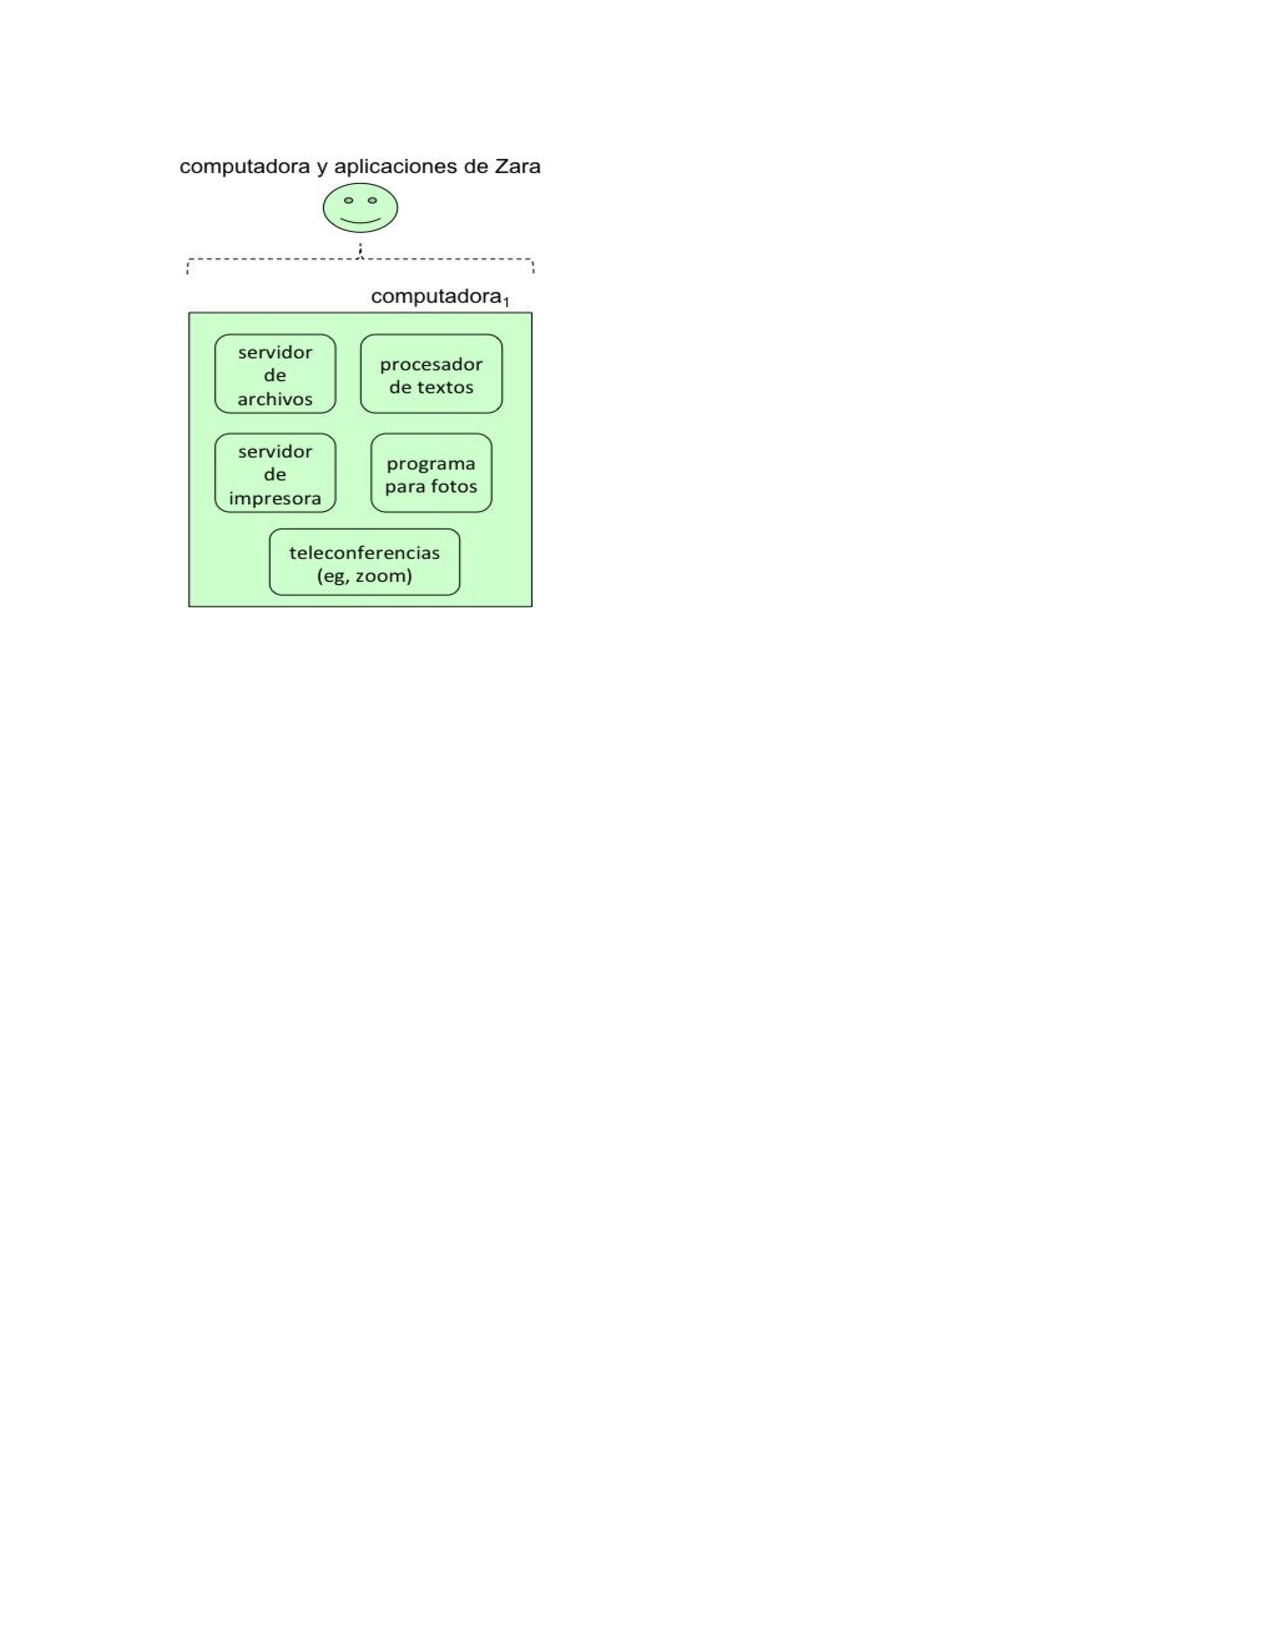
\includegraphics[width=0.85\columnwidth]{imagenes/imagendesc1.pdf}
\caption{Representación conceptual de sistema centralizado.}
\label{imagendesc1}
\end{figure} 

La figura 1 muestra la representación conceptual de un sistema centralizado. Para simplificar la explicación, esta figura supone que el mismo pertenece a una sola persona (Zara). 

El sistema centralizado de Zara se compone de una sola computadora (compu1) en la cual Zara ha instalado todas sus aplicaciones: servidor de archivos, procesador de textos, servidor de impresora, programa de fotos, teleconferencias. 

\section{Sistema distribuido (distributed system)}

Un sistema distribuido es aquel que se compone de varios dispositivos y varias aplicaciones (también llamadas funciones) instaladas dispersamente y posiblemente replicadas dos o más veces, en dichos dispositivos. 

La principal característica de estos sistemas es que el o los propietarios/s no instalan todas las aplicaciones en un solo lugar.  

Destacamos que la distribución se refiere a la arquitectura del sistema, por lo tanto, pensamos que posiblemente deberían llamarse \textbf{sistemas de arquitectura distribuida}. El uso de esta terminología dejaría claro que la denominación no contempla quien controla el sistema, es decir quién es el propietario o administrador; bajo esta definición, ese punto es irrelevante. Al contrario, es conveniente mencionar que, al instalar las aplicaciones en varios dispositivos, el sistema es más robusto: si alguno de los dispositivos se satura, se apaga, queda fuera de conexión o falla, el sistema sigue funcionando. Lo hará parcialmente y probablemente sin alteración, siempre que exista una réplica de la aplicación en otro dispositivo.


\begin{figure}
\centering
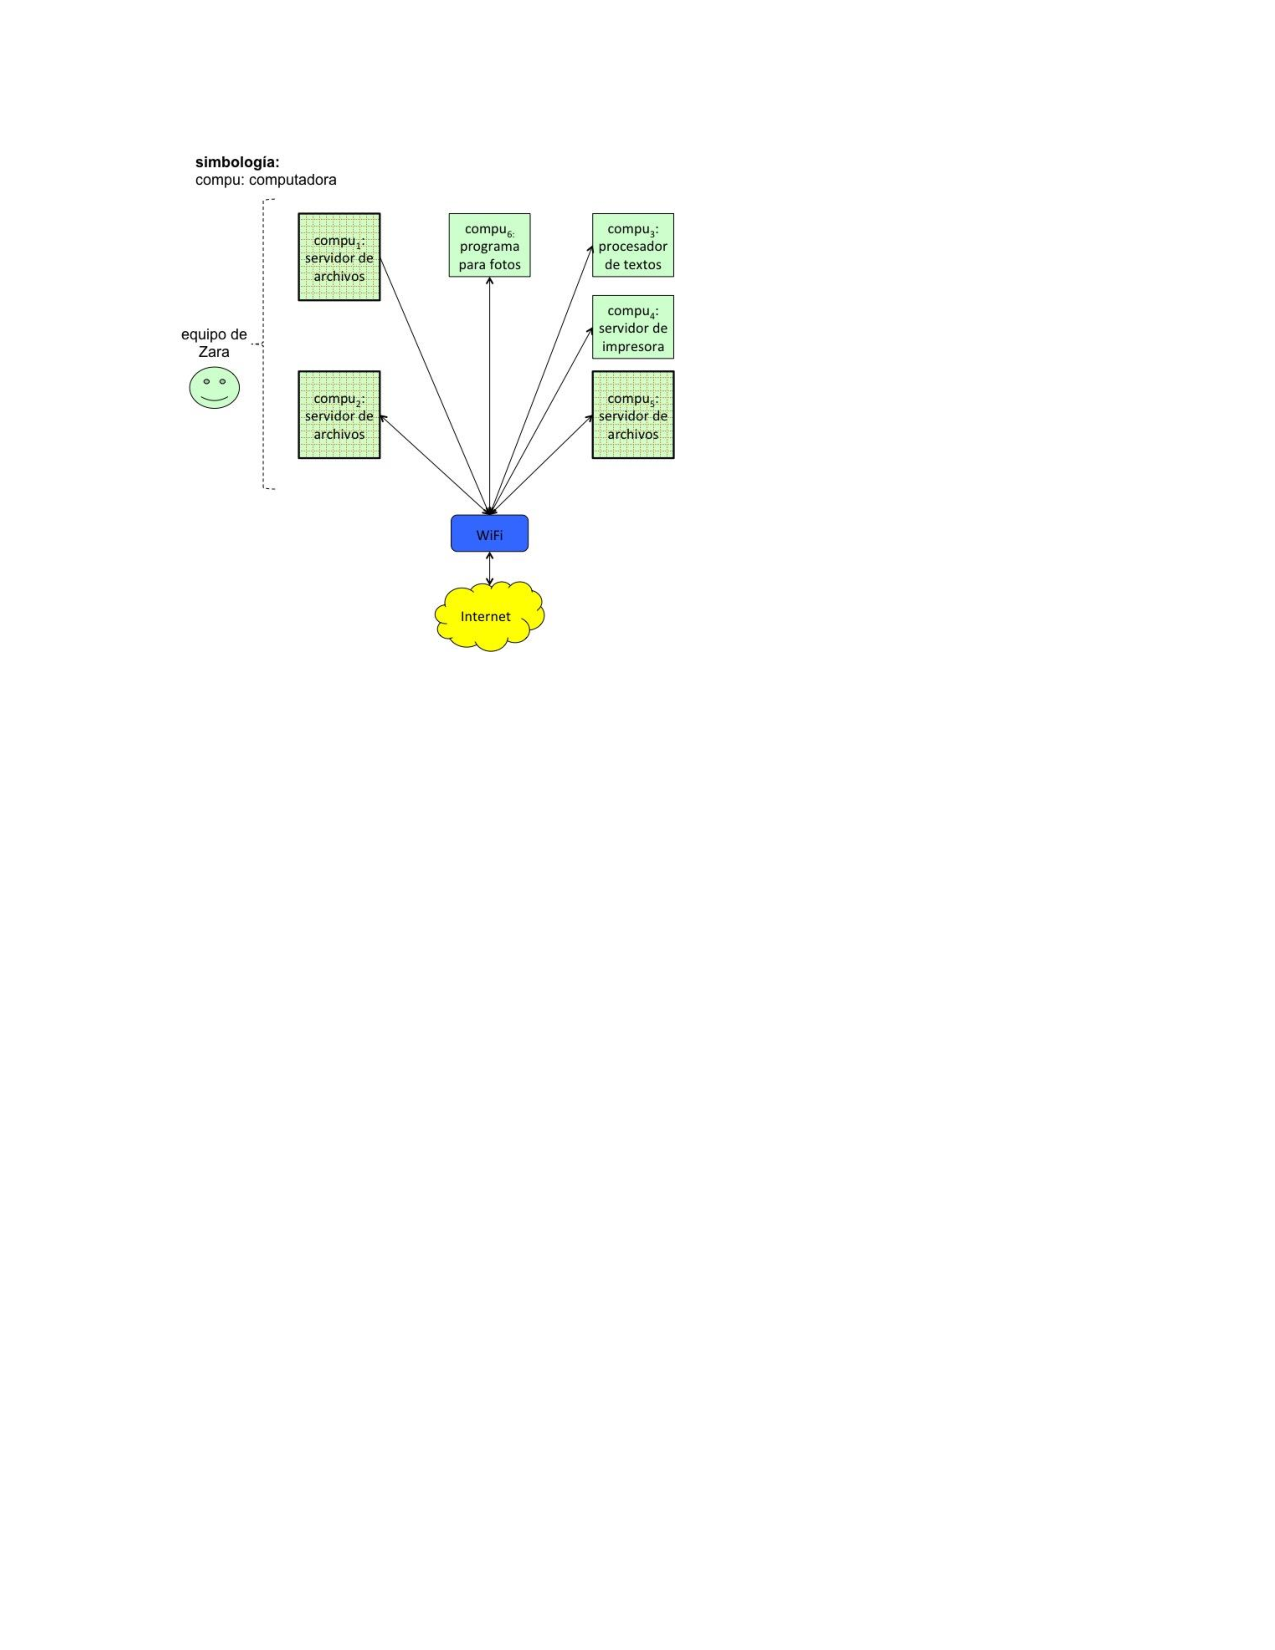
\includegraphics[width=0.85\columnwidth]{imagenes/imagendesc2.pdf}
\caption{Representación conceptual de sistema distribuido.}
\label{imagendesc2}
\end{figure} 

Utilizaremos la figura 2 para explicar el concepto antes mencionado. Esta figura muestra el sistema de Zara referido en la figura 1, pero esta vez instalado de manera distribuida. Nuevamente, para facilitar la exposición asumimos que las seis computadoras del sistema pertenecen a Zara. Obsérvese que Zara ha instalado tres réplicas de su servidor de archivos en sus computadoras compu1, compu2 y compu5. Para resaltar las réplicas hemos marcado las tres computadoras con un fondo cuadrado y líneas gruesas. Zara ha colocado las demás aplicaciones en las otras computadoras: su programa para fotos (compu6,), el procesador de textos (compu3) y el servidor de impresora (compu4). Gracias a esta distribución de aplicaciones, Zara tiene un sistema más robusto, si falla su compu6 ella se queda sin poder mirar sus fotos, pero puede seguir trabajando. Si falla la compu4 no podrá imprimir, pero puede seguir trabajando y lo más notable, si falla la compu2, Zara no sufre contratiempos, su compu1 y compu5 tienen copias de los archivos. Zara se quedaría sin poder leer sus archivos si fallaran al mismo tiempo las compu1 compu2 y compu5, pero esto es muy poco probable que suceda. 

\section{Sistemas centralizados y descentralizados \textbf{(centralized and decentralise systems)}}

Desde el punto de vista administrativo, los sistemas (plataformas) se pueden dividir en: centralizados y descentralizados.

\section{Sistema centralizado (centralized system)}

Un sistema centralizado es aquel que se encuentra bajo el control de una sola autoridad.

La principal característica de estos sistemas es que el propietario actúa como autoridad central y como tal tiene la responsabilidad de mantener el sistema activo y los derechos de dictar las políticas relativas a su funcionamiento. Por ejemplo, quién, cuándo y bajo qué condiciones lo puede usar.

Es importante resaltar que la centralización se refiere solamente al aspecto administrativo del sistema; por lo tanto, quizá estos sistemas deberían llamarse \textbf{sistemas de administración centralizada} o \textbf{sistemas de mando centralizado}. De esta forma, se dejaría en claro que el concepto no contempla la arquitectura técnica del sistema, es decir, cómo y dónde (en uno o varios dispositivos) están instaladas las aplicaciones. Bajo esta denominación, el aspecto técnico es irrelevante. 

Al contrario, es fundamental que, al estar todas las aplicaciones bajo una sola autoridad, éstas se encuentran a expensas de las decisiones administrativas de la misma. De esta manera, si la autoridad ordena desactivar alguna de las funciones, aquellas quedarían fuera del alcance de los usuarios, y aún peor, si decide apagar completamente el sistema, se quedarían completamente sin sistema. 


Esta figura \ref{imagendesc3}

\begin{figure}
\centering
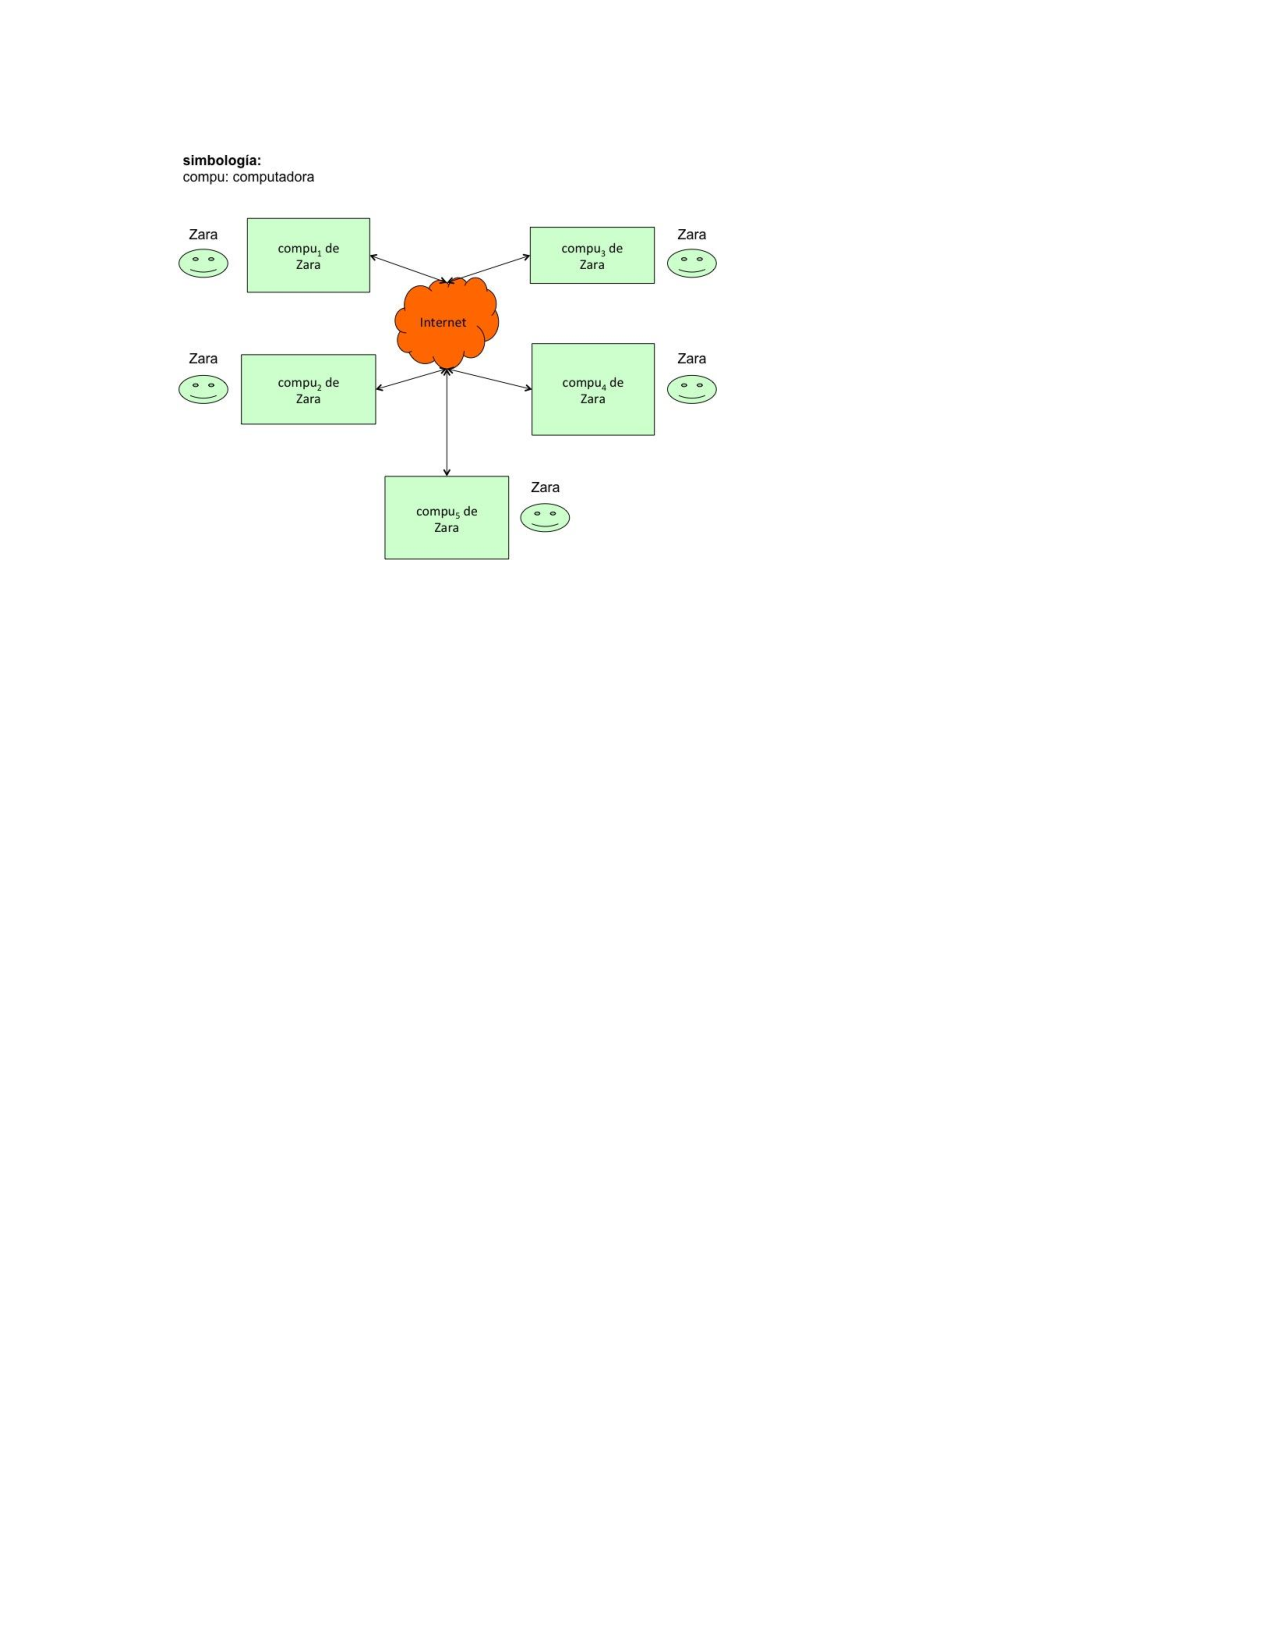
\includegraphics[width=0.85\columnwidth]{imagenes/imagendesc3.pdf}
\caption{Representación conceptual de sistema de administración centralizada.}
\label{imagendesc3}
\end{figure} 

La figura 3 expone el concepto de sistemas centralizados, en efecto, de un sistema de administración centralizado. El sistema, en la ilustración, está compuesto de cinco computadoras pertenecientes a Zara. Para simplificar, consideramos que Internet no es parte de dicho sistema. La figura no específica qué aplicación o aplicaciones ha instalado Zara en sus computadoras; esto es secundario, por el momento importa mencionar solo la parte administrativa. El tema de la aplicación instalada en el ejemplo, lo retomaremos cuando hablemos de blockchains.

\section{Sistema descentralizado (descentralized system)}

Un sistema descentralizado es aquel que no se encuentra bajo el control de una sola autoridad.

La principal característica de estos sistemas es que, al carecer de autoridad central, todos los participantes tienen el mismo status e interactúan bajo el modelo que se conoce como de uno a uno o entre iguales \textit{(peer-ro-peer)}.  

Aclaramos que la descentralización se refiere solamente al aspecto administrativo del sistema, por lo tanto, a nuestro entender estos sistemas deberían llamarse \textbf{sistemas de administración descentralizada} o \textbf{sistemas de mando descentralizado}. Dicha denominación no contempla la arquitectura técnica del sistema, es decir cómo y dónde (en uno o varios dispositivos) están instaladas las aplicaciones. Bajo esta conceptualización, el aspecto técnico es irrelevante. 

Al contrario, es esencial resaltar que, en estos sistemas nadie tiene la responsabilidad de mantenerlos funcionando, ni el derecho de dictar las políticas de operación. En los sistemas descentralizados nadie tiene el derecho, ni los mecanismos técnicos para imponer condiciones; por ejemplo, quién, cuándo y bajo qué condiciones pueden los usuarios usar el sistema. El funcionamiento de las aplicaciones está fuera del alcance de una autoridad central. No existe una autoridad que pueda desactivar el sistema, ni siquiera alguna de sus aplicaciones.


Esto esta en \ref{fig:imagendesc4}
 
\begin{figure}
\centering
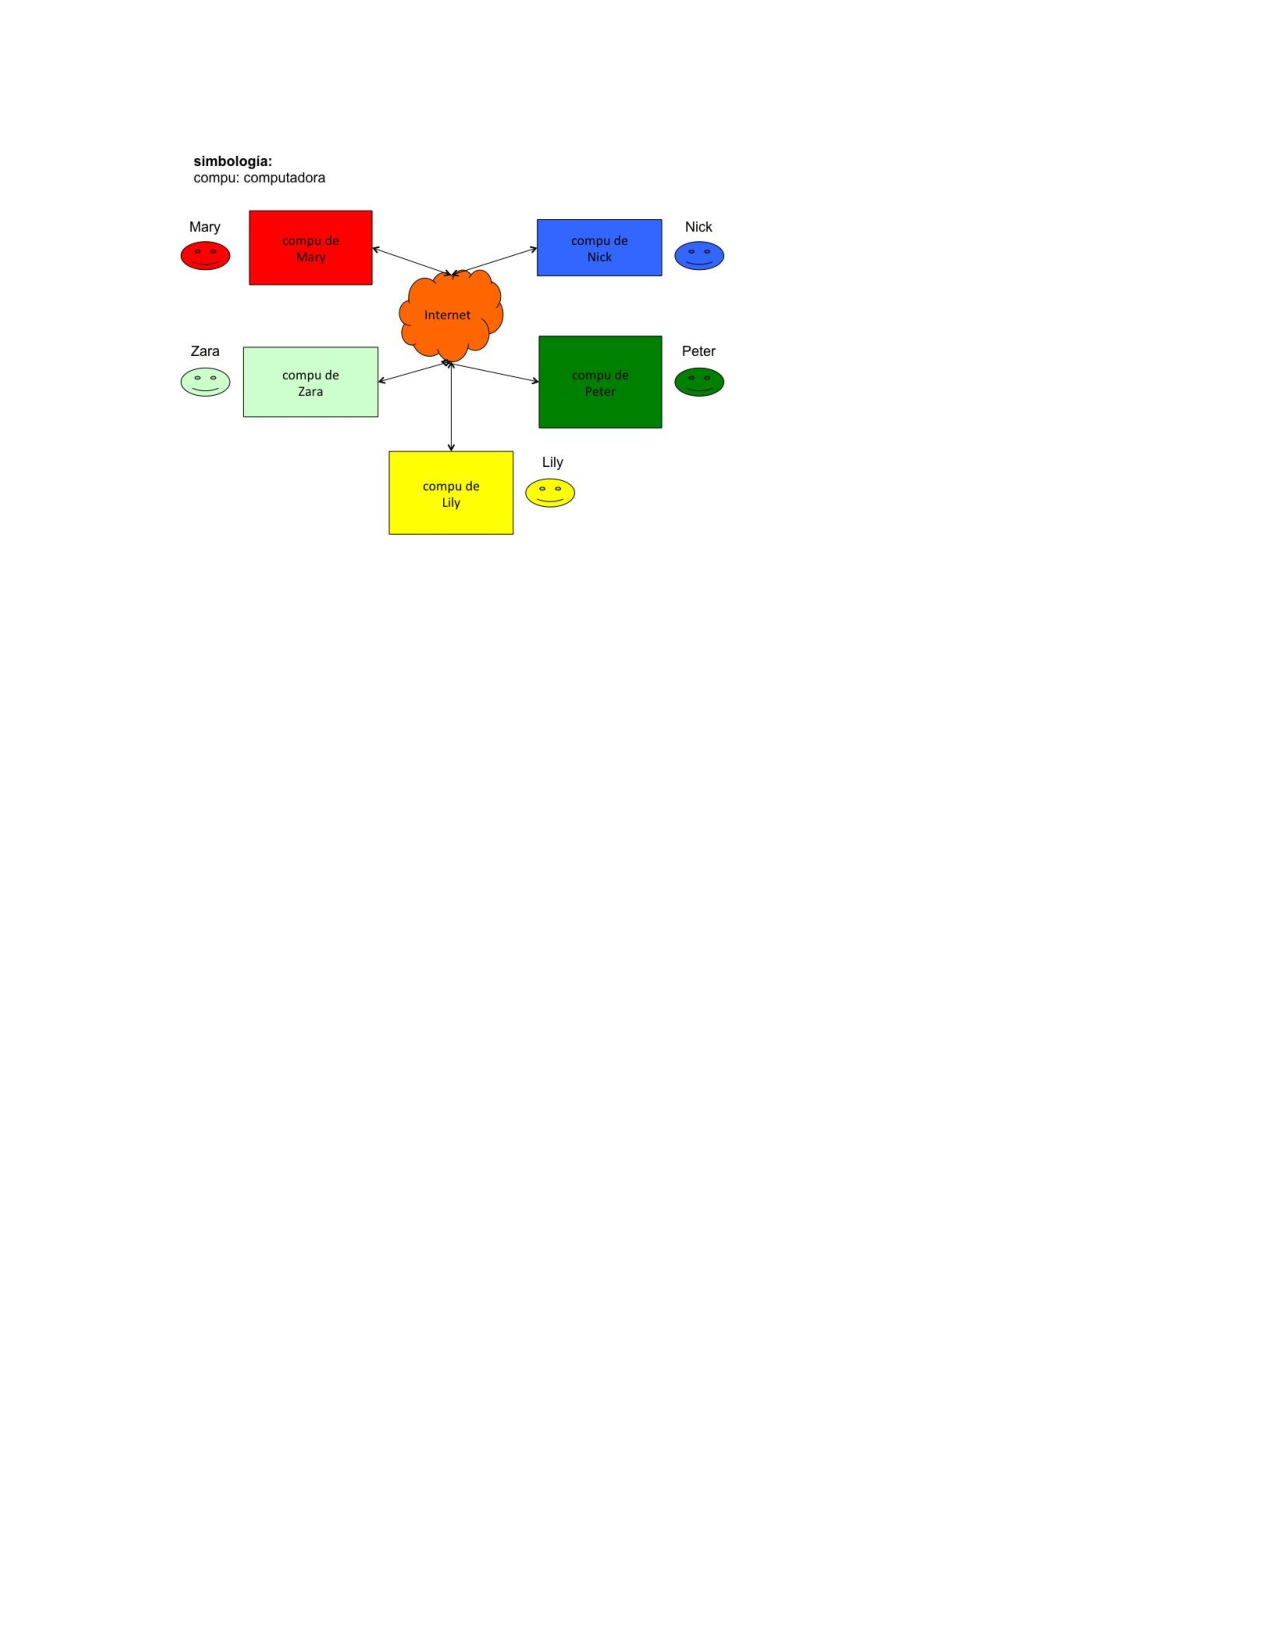
\includegraphics[width=0.85\columnwidth]{imagenes/imagendesc4.pdf}
\caption{Representación conceptual de sistema de administración descentralizada.}
\label{fig:imagendesc4}
\end{figure} 


La figura 4 explica el concepto de un sistema descentralizado, concretamente, de un sistema de administración descentralizada. El sistema de la ilustración es el mismo que el de la figura 3, excepto que en el ejemplo de la figura 4, las cinco computadoras pertenecen a varios propietarios: la computadora roja pertenece a Mary, la verde a Zara, la amarilla a Lilly, etc.  Para simplificar, consideramos que Internet no es parte del sistema. La figura no especifica qué aplicación o aplicaciones han instalado Mary, Zara, Lilly, Peter y Nick en sus computadoras, esto no es relevante, por el momento importa aclarar solo la parte administrativa. El tema de la aplicación instalada en la figura 3, lo retomaremos cuando hablemos de blockchains. Continuando con el ejemplo, Zara es propietaria de una computadora, como tal, ella tiene control de su computadora, pero no tiene autoridad alguna sobre las otras. Todos los participantes, tienen el mismo status y control de sus respectivas computadoras; por ejemplo, Nick puede desactivar temporal o permanentemente su computadora azul sin consultar o pedir permiso a nadie. 

Un sistema completamente descentralizado tiene un número de propiedades en términos de escala y resiliencia, como veremos más adelante. La descentralización permite una gestión local independiente de la global, lo que significa que la diversidad y la heterogeneidad ocurren naturalmente.\footnote{Jon Crowcroft, Jon, “FIE - Future Internet Enervation” , The Computer Laboratory, University of Cambridge Cambridge}  Sin embargo, un sistema con estructura descentralizada puede no serlo totalmente, Como expresa  \footnote{Crowcroft, Jon, Tyson, Gareth, Mortier, Richard, “Redhouse Gases – A manifesto for re-decentralization”, University of Cambridge, diciembre 2020 }, las redes tienen una tendencia hacia la centralización de datos y de ahí a la concentración de poder, si bien tenemos las herramientas para reconstruir sistemas en una forma de igual a igual (peer to peer). Simplemente pensemos en las plataformas que funcionan como intermediarios entre las partes generando no pocas implicancias jurídicas (en el capítulo de contratos automáticos abordamos en detalle este tema). Para ejemplificar, consideremos el caso de las plataformas de financiamiento artístico donde el mecenas y el artista tienen una relación contractual con la plataforma que media entre ellos. 

Los sistemas descentralizados proporcionan una latencia\footnote{En redes informáticas de datos, la latencia de red es la suma de retardos temporales dentro de una red. Un retardo es producido por la demora en la propagación y transmisión de paquetes dentro de la red. \url{https://es.wikipedia.org/wiki/Latencia}}  más baja, un menor consumo de energía y una mayor privacidad para los usuarios. Por lo tanto, pueden proporcionar más eficacia y negociabilidad.\footnote{\cite{JonGareth2020}, “Redhouse Gases – A manifesto for re-decentralization”} 

Ahora bien, si todas las blockchain son distribuidas, entonces la siguiente pregunta es: ¿de quiénes son las computadoras que usan las blockchain? La respuesta podría ser:

\begin{itemize}
    \item De una sola persona: entonces la blockchain será centralizada porque existe una persona que controla todo.
    \item De varios propietarios: entonces la blockchain será descentralizada porque no hay una sola persona que controle todo.
\end{itemize}

Podemos visibilizarlo mejor con los siguientes ejemplos que, si bien son poco factibles en la realidad, pueden ayudarnos a comprender la temática. Luego haremos analogías:

Imaginemos el sistema de taxis de una ciudad. Si hubiese un solo taxi, sería muy arriesgado dado que, si el automóvil se descompone hoy, se acaba el servicio. Para evitar este problema, se colocan varios taxis a trabajar (compus). Si ya tienes cientos de taxis funcionando, la pregunta es de quiénes son todas esos taxis:

\begin{itemize}
    \item de un solo dueño: ese solo dueño tiene el control total, centraliza todo, impone condiciones.
    \item de cientos de dueños: no hay una sola persona que tenga el control absoluto e imponga tarifas.
\end{itemize}

Algo similar sucede con la generación de energía para los hogares: en muchos países, el sistema es centralizado, una o dos compañías controlan todo, solo ellos la generan y la venden. Una opción, a fin de evitar el monopolio sería descentralizar: que los dueños de los hogares tengan posibilidad de generar su propia energía y en caso de existir un remanente puedan hasta venderla. En este caso, no hay una persona o empresa que centralice y controle todo. Allí reside todo el atractivo y el problema de los sistemas descentralizados.

\subsection{Consolidación de la Internet}

Un concepto del que se habla mucho en la actualidad y que está relacionado con el tema de la descentralización es el de la consolidación de la Internet \textbf{(Internet Consolidation)}

La \textbf{consolidación de la Internet} se define como un proceso de desarrollo que provocó que gran parte de la infraestructura básica y de servicios se encuentren bajo el control de un pequeño grupo de empresas. Por infraestructura aquí entendemos la base tecnológica sobre la que Internet funciona y que por lo regular pasa desapercibida para el usuario, como puede ser la distribución de contenido. Ejemplos de servicios son los buscadores (google), correos (gmail) y redes sociales (facebook) con los que el usuario interactúa directamente.

Mencionamos el tema de la consolidación de la Internet en esta sección debido a que existen ciertos autores que cuestionan si las plataformas de blockchain pueden en un futuro, no ser o quizás ya han sido afectadas por este proceso económico a través de la acción de los mineros.  Se habla de que en la competición del proceso de mineros de Bitcoin solamente algunas personas (los llamados mining pools) que han adquirido computadoras ponderosas y diseñadas específicamente para participar en dichos procesos, pueden competir.     

Sin duda, en la consolidación de la Internet intervienen ciertos factores, entre ellos el económico\footnote{Arkko Jari, “The influence of internet architecture on centralised versus distributed internet services”, Journal of Cyber Policy, volumen 5, numero 1, 2021, \url{https://doi.org/10.1080/23738871.2020.1740753}} y varios efectos negativos como el oligopolio.  Para dar una idea basta mencionar que, en la actualidad, Google y Facebook, son propietarios de aproximadamente 84\% de los anuncios en el mercado chino. Amazon es dueña de 41.1\% del Mercado en línea de USA y Alibaba de más del 60\% del de China. Además, 90\% de las búsquedas en Internet se hacen con Google.\footnote{Arkko, J., Trammell,B., Nottingham, N., Huitema, C, Thomson M., Tantsura, J,, Oever, N., “Considerations on Internet Consolidation and the Internet Architecture”,Ietf,draft-arkko-iab-internet-consolidation-02, jul, 2019, \url{https://tools.ietf.org/pdf/}} 

\subsection{Desafíos de los sistemas descentralizados}

La descentralización trae consigo una serie de desafíos, tales como:

\textbf{Disponibilidad} Existen dos desafíos para proporcionar alta disponibilidad a partir de la computación y el almacenamiento descentralizado. Primero, la posibilidad de conectarse a una red. Segundo, menor cantidad de fallas de los enlaces domésticos. Las medidas varían, pero pueden ocurrir interrupciones típicas de horas. Exponiendo el control sobre éste permitiría a las personas mejorar su conectividad para atender sus propias necesidades.

A medida que Internet se actualiza, vemos un movimiento hacia una mayor implementación de fibra hasta el hogar en regiones desarrolladas, o redes 5G, donde la capacidad es mucho más alta, por lo que las velocidades de enlace ascendente pueden ser relevantes y la disponibilidad y latencia también puede mejorar significativamente. Sin embargo, tenemos mucha heterogeneidad en el sistema y siempre habrá enlaces mucho más lentos, y máquinas menos fiables en el hogar.

La forma habitual de evitar esta situaciòn es mediante la replicación. De hecho, los servicios centralizados en la nube ya implementan la replicación, dentro de los centros de datos y entre los centros de datos a través de la red de área amplia. Los mismos algoritmos se pueden aplicar en la nube de forma descentralizada. En realidad, investigaciones recientes sobre algoritmos de consenso (ej. Paxos flexibles) permiten ajustar el protocolo para que las actualizaciones del estado (contenido mutable o cálculo) se apliquen de manera consistente en todas las copias, incluso en el área amplia. Además, podemos sintonizar copias que se ejecutan en sitios dispares. 

\textbf{Incentivos} Si bien existe un motivo para que las personas participen en el intercambio mutuo, esto puede fallar en un mundo con comportamientos bizantinos. Los libros de contabilidad distribuidos para las criptomonedas se han basado en varios enfoques de prueba de trabajo insostenibles. Tampoco esto ha evitado ataques de colusión. En un nivel superior, se encuentran los incentivos para el innovador, ya sea para quienes quieren ampliar su sistema rápidamente y, por lo tanto, aprovechan sustratos centralizados (la nube), o bien para aquellos que están preparados para una ventaja larga y lenta en el tiempo, y por lo tanto, prefieren dejar que un sistema descentralizado crezca de manera más orgánica.  

\textbf{Integridad} Los primeros sistemas de intercambio de archivos punto a punto sufrían ataques que atentaban contra su integridad. Es un desafío construir verificaciones de integridad sin invocar un oráculo o un servidor centralizado. 

\textbf{Identidad} Hay una variedad de ataques a la identidad en sistemas descentralizados con cuentas falsificadas y replicadas (por ejemplo, los ataques de Sybil).  Es un desafío articular los medios necesarios para que los sistemas descentralizados brinden mayor protección y seguridad  a fin de evitar  ciertos delitos, tales como fraudes y falsificaciones.

\section{BLOCKCHAIN}
\label{Blockchain}

\subsection{Resumen}




\begin{figure}
\centering
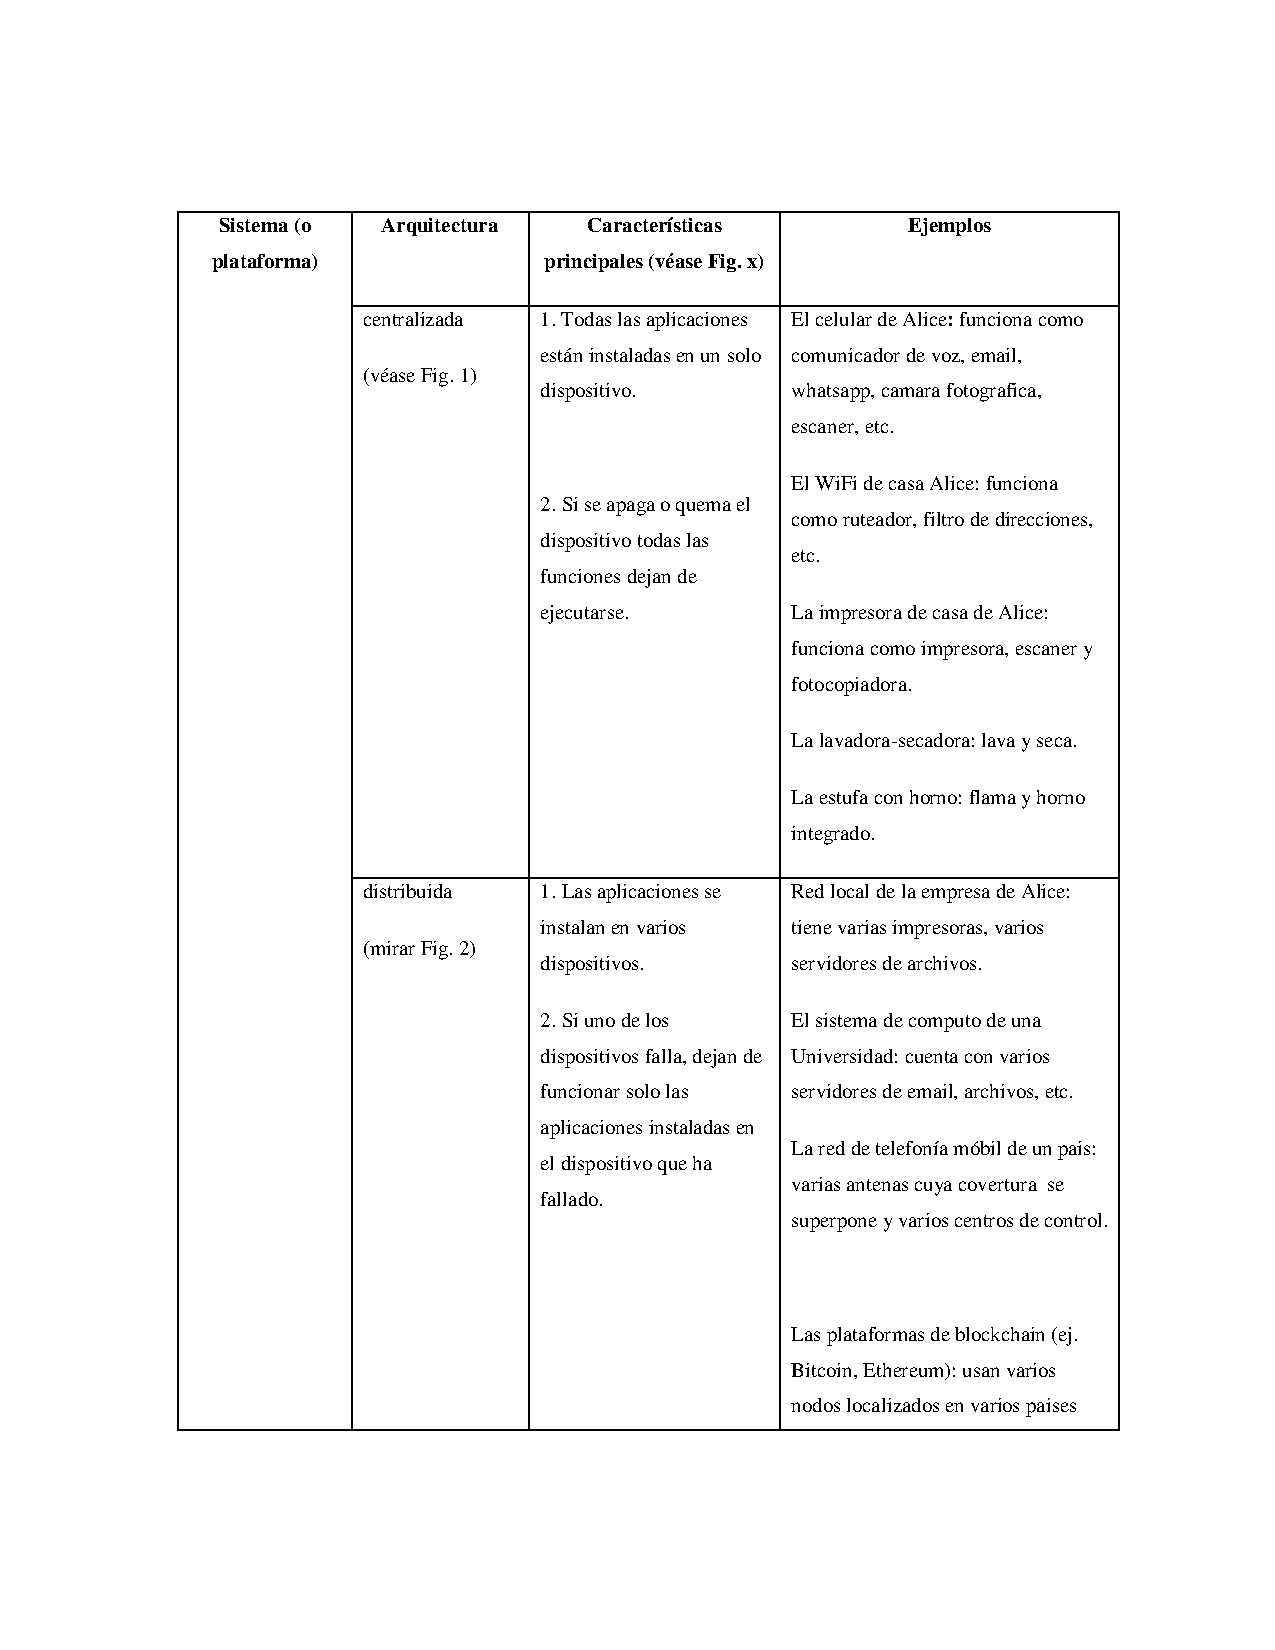
\includegraphics[width=0.85\columnwidth]{imagenes/imagendesc5.pdf}
\caption{RSistemas de arquitectura centralizada y distribuida}
\label{imagendesc5.pdf}
\end{figure} 

Esta figura \ref{imagendesc6}

\begin{figure}
\centering
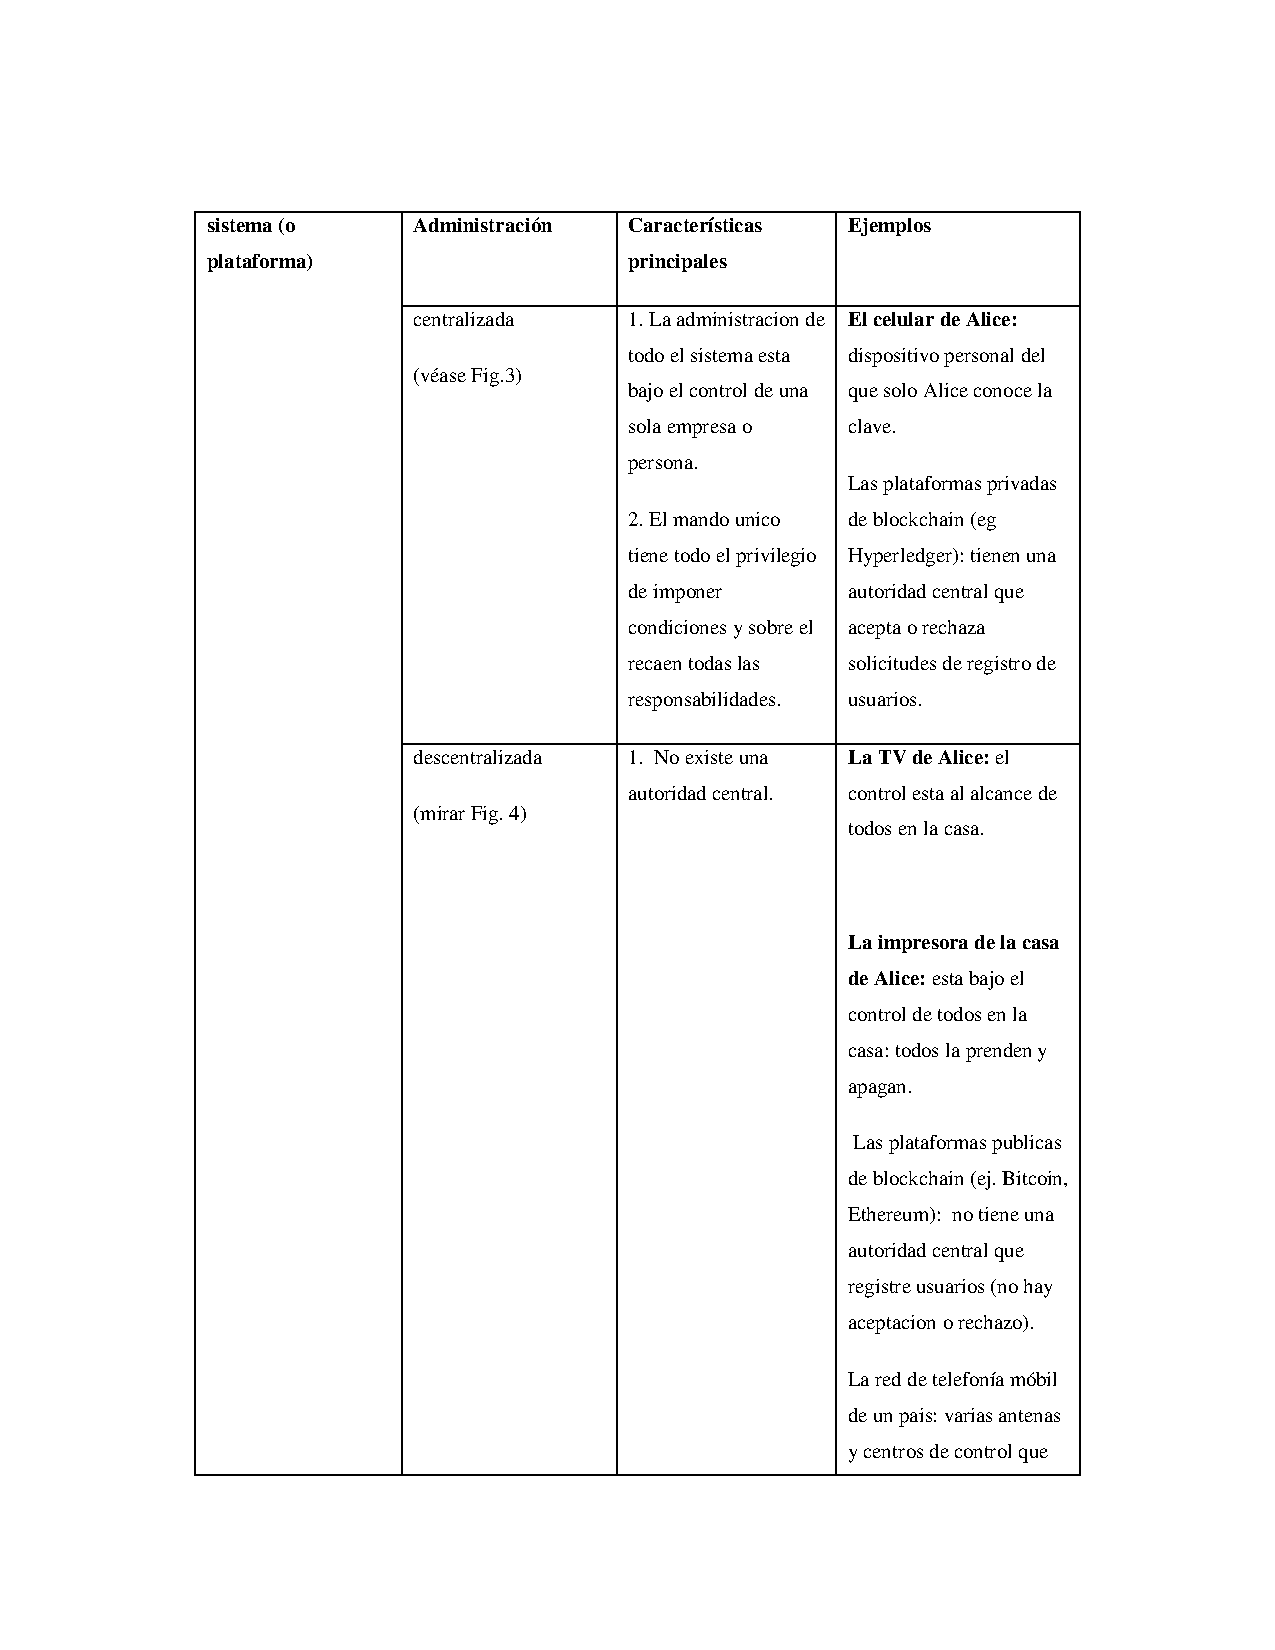
\includegraphics[width=0.85\columnwidth]{imagenes/imagendesc6.pdf}
\caption{Sistemas de administración centralizada y descentralizada}
\label{imagendesc6}
\end{figure} 

Las cuatro variantes de sistemas (de arquitectura centralizada y distribuida y sistemas de administración centralizada y descentralizada) pueden combinarse para formar sistemas con varias características. La tabla 3 muestra las combinaciones posibles.

Esta figura \ref{imagendesc7).pdf}


\begin{figure}
\centering
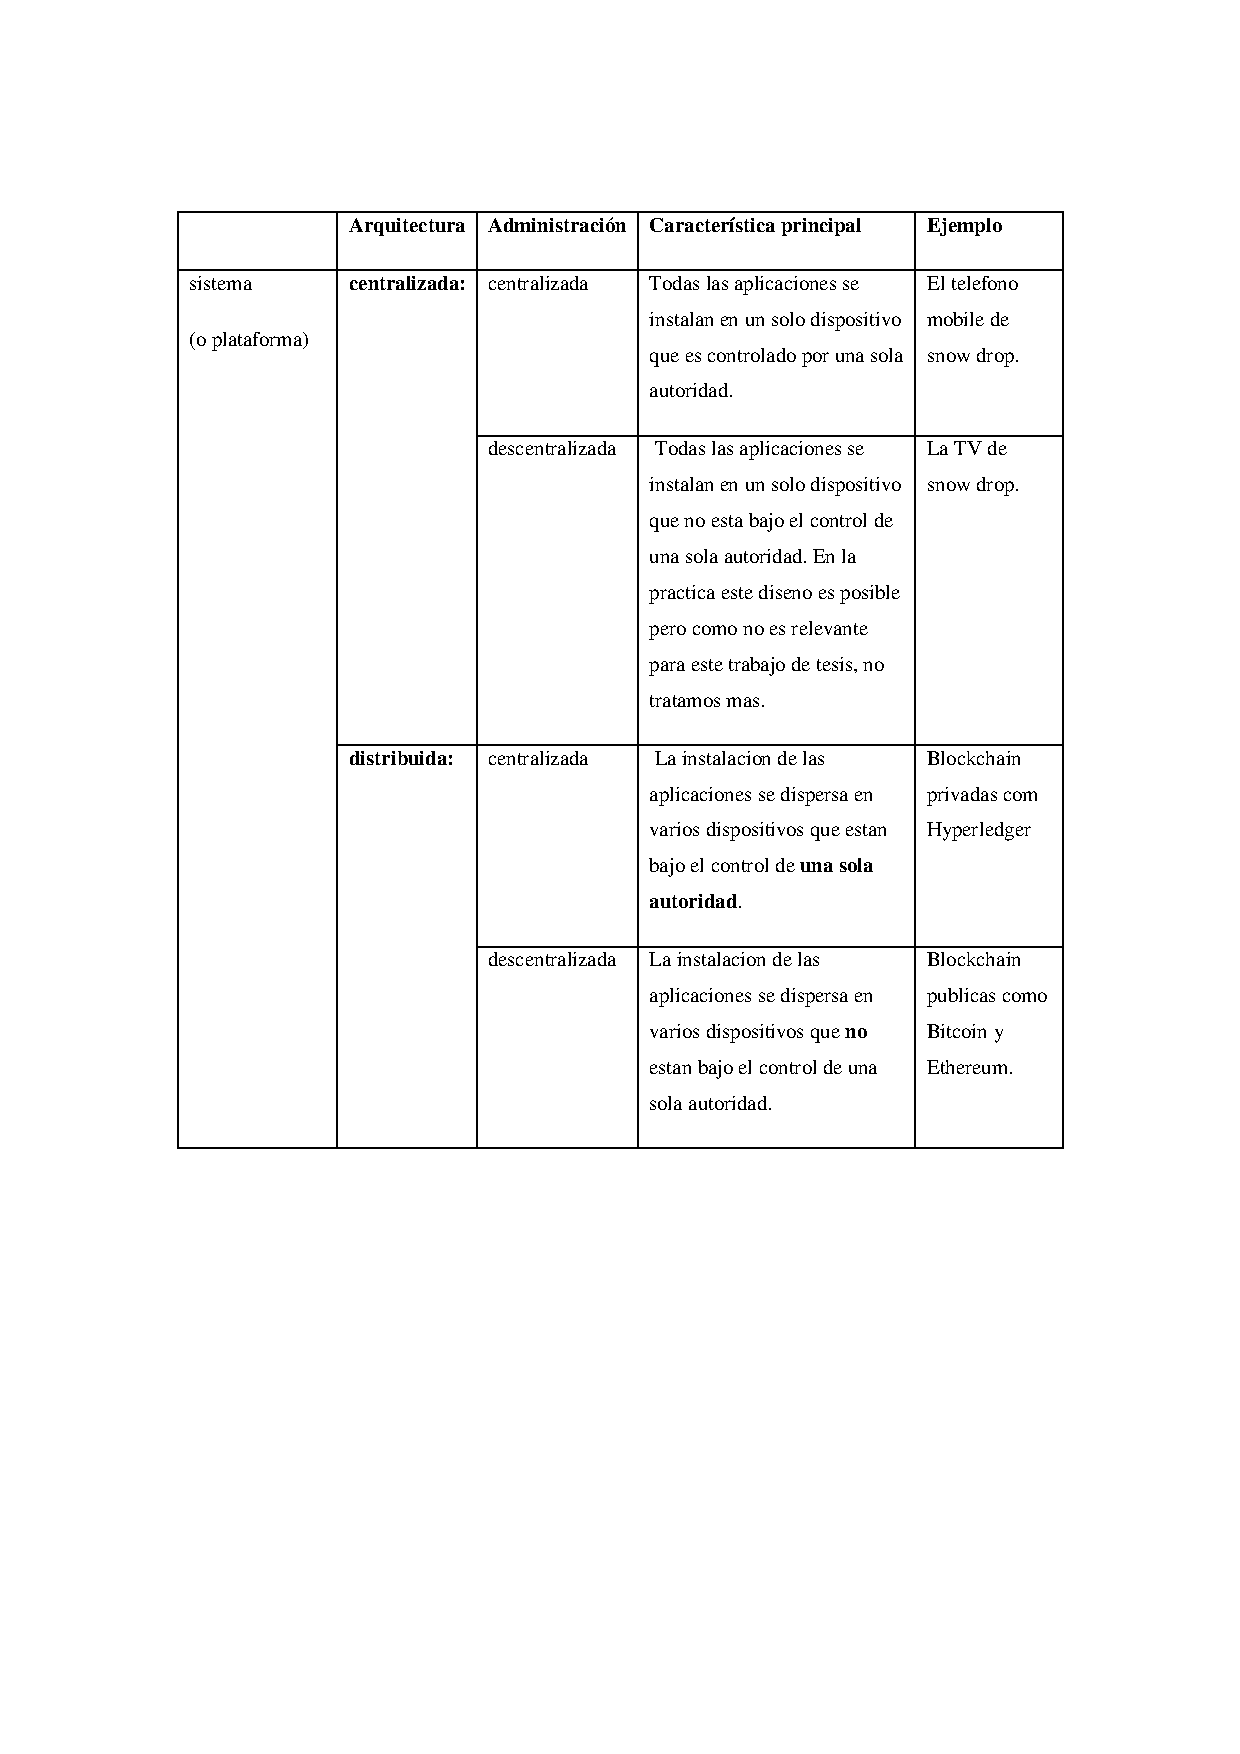
\includegraphics[width=0.85\columnwidth]{imagenes/imagendesc7).pdf}
\caption{Sistemas de arquitectura centralizada y distribuida y sistemas  de administración centralizada y descentralizada.}
\label{imagendesc7).pdf}
\end{figure} 


\chapter{Seguridad, Protección de documentos y Firmas}
\label{Seguridad, Protección de documentos y Firmas}

\section{1.	Tecnología digital, codificación y archivos digitales}

La tecnología digital no sólo ha cambiado la forma en que se celebran y ejecutan los contratos (como hemos visto en el capítulo XX), sino que también ha variado la forma de firmarlos. Esta innovación que desarrollaremos seguidamente ha producido nuevos desafíos en el ámbito legal. 

Podemos decir que la tecnología digital se refiere a una rama de la electrónica que codifica la información usando solamente dos dígitos: el 0 (cero) y el 1 (uno).  A cada dígito se le llama “bit” y al código que resulta se le llama código binario. Por ejemplo, el número “5” que vemos en el teclado, se codifica en código binario como 00000101, la letra “a” que vemos en el teclado se codifica en código binario como 0110 0001. La palabra “ … ” se codificaría como 01010011 01100001 01101110 01100100 01110010 01100001.  

Las computadoras actuales utilizan tecnología digital y, por ende, códigos binarios, como los ejemplos arriba citados para codificar la información que manejan. Vale la pena mencionar que, para facilitar sus operaciones, utilizan también otros códigos. Por ejemplo, el código hexadecimal en donde, el número “5”, la letra “a” y la palabra “ … ” se representan como: 35, 61 y …, respectivamente.  Existen convertidores de códigos en línea, por ejemplo \url{https://www.online-toolz.com/tools/text-hex-convertor.php}. Estos códigos son estándares y son comprendidos por los que a estos temas se dedican. Se les conoce como códigos de computadoras y todos ellos son equivalentes. Es decir, se pueden convertir fácilmente de uno a otro.

Aclaramos que el resultado, por ejemplo, al codificar la palabra “… ” en código binario  (01010011 01100001 01101110 01100100 01110010 01100001), el resultado no es un código secreto y no se debe confundir con los códigos criptográficos.

Definimos “codificar” como la operación para representar información en un código de computadora.

La tecnología ahora permite codificar objetos multimedia (texto, fotos, videos, etc.) que anteriormente podíamos representar solamente en medios físicos. La codificación de un objeto genera un archivo que se conoce como archivo digital haciendo referencia a la tecnología que se emplea para generarlo y manipularlo (editarlo, borrarlo, comprimirlo, enviarlo, etc.). Por ejemplo, podemos codificar un documento tradicional como una carta escrita en una hoja tamaño carta y guardarlo en un archivo, lo mismo podemos hacer con un libro de 200 páginas y guardarlo en un archivo, una pieza musical, una foto, una obra de arte, etc. Para proteger un archivo se puede utilizar un \textbf{“hash”}.\footnote{Hash: es una operación criptográfica que un usuario, por ejemplo Bob, puede aplicarle a un archivo (documento doc.txt) para evitar que alguien altere el documento sin que Bob pueda detectarlo. }  En la práctica se conoce bajo diferentes nombres (digital finger print, etc.). Vale la pena aclarar que se usa para proporcionar solamente integridad; es decir, no proporciona confidencialidad porque el documento no queda encriptado (ilegible). 

Esta figura \ref{imagenfirma1}


\begin{figure}
\centering
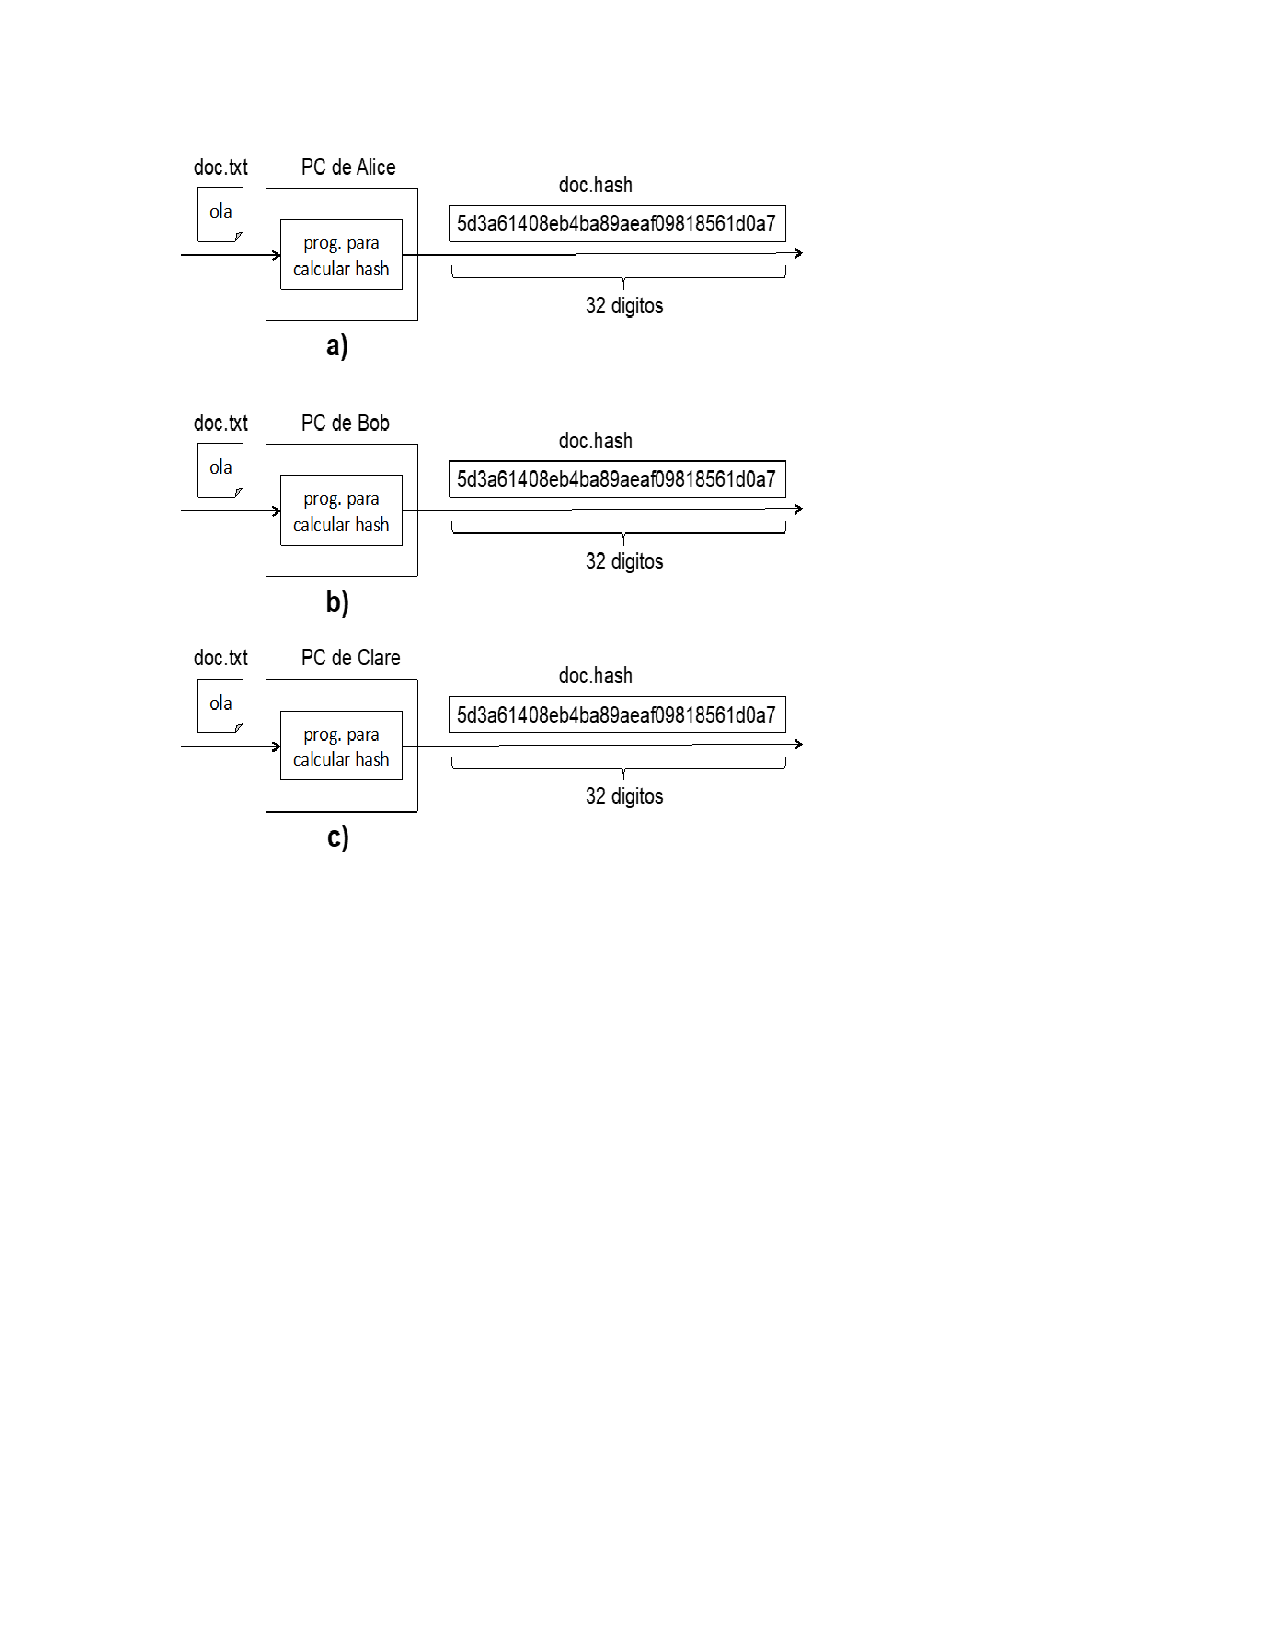
\includegraphics[width=0.85\columnwidth]{imagenes/imagenfirma1.pdf}
\caption{Concepto de hash.}
\label{imagenfirma1}
\end{figure} 

Importa resaltar que la longitud del hash es siempre un número fijo (por ej. 32, 64, 256, etc.) dependiendo del standard que se use) independientemente de la longitud del archivo de entrada. 

Es importante destacar que el hash que se obtiene a la salida del programa por ejemplo 5d3a61408eb4ba89aeaf09818561d0a7 en Fig X, es solo una cadena de dígitos que sella el contenido del archivo doc.txt para impedir que sea modificado, por ende, no es posible recuperar el contenido del archivo doc.txt a partir del hash, esa no es su función.

Esta figura \ref{gatorojo}

\begin{figure}
\centering
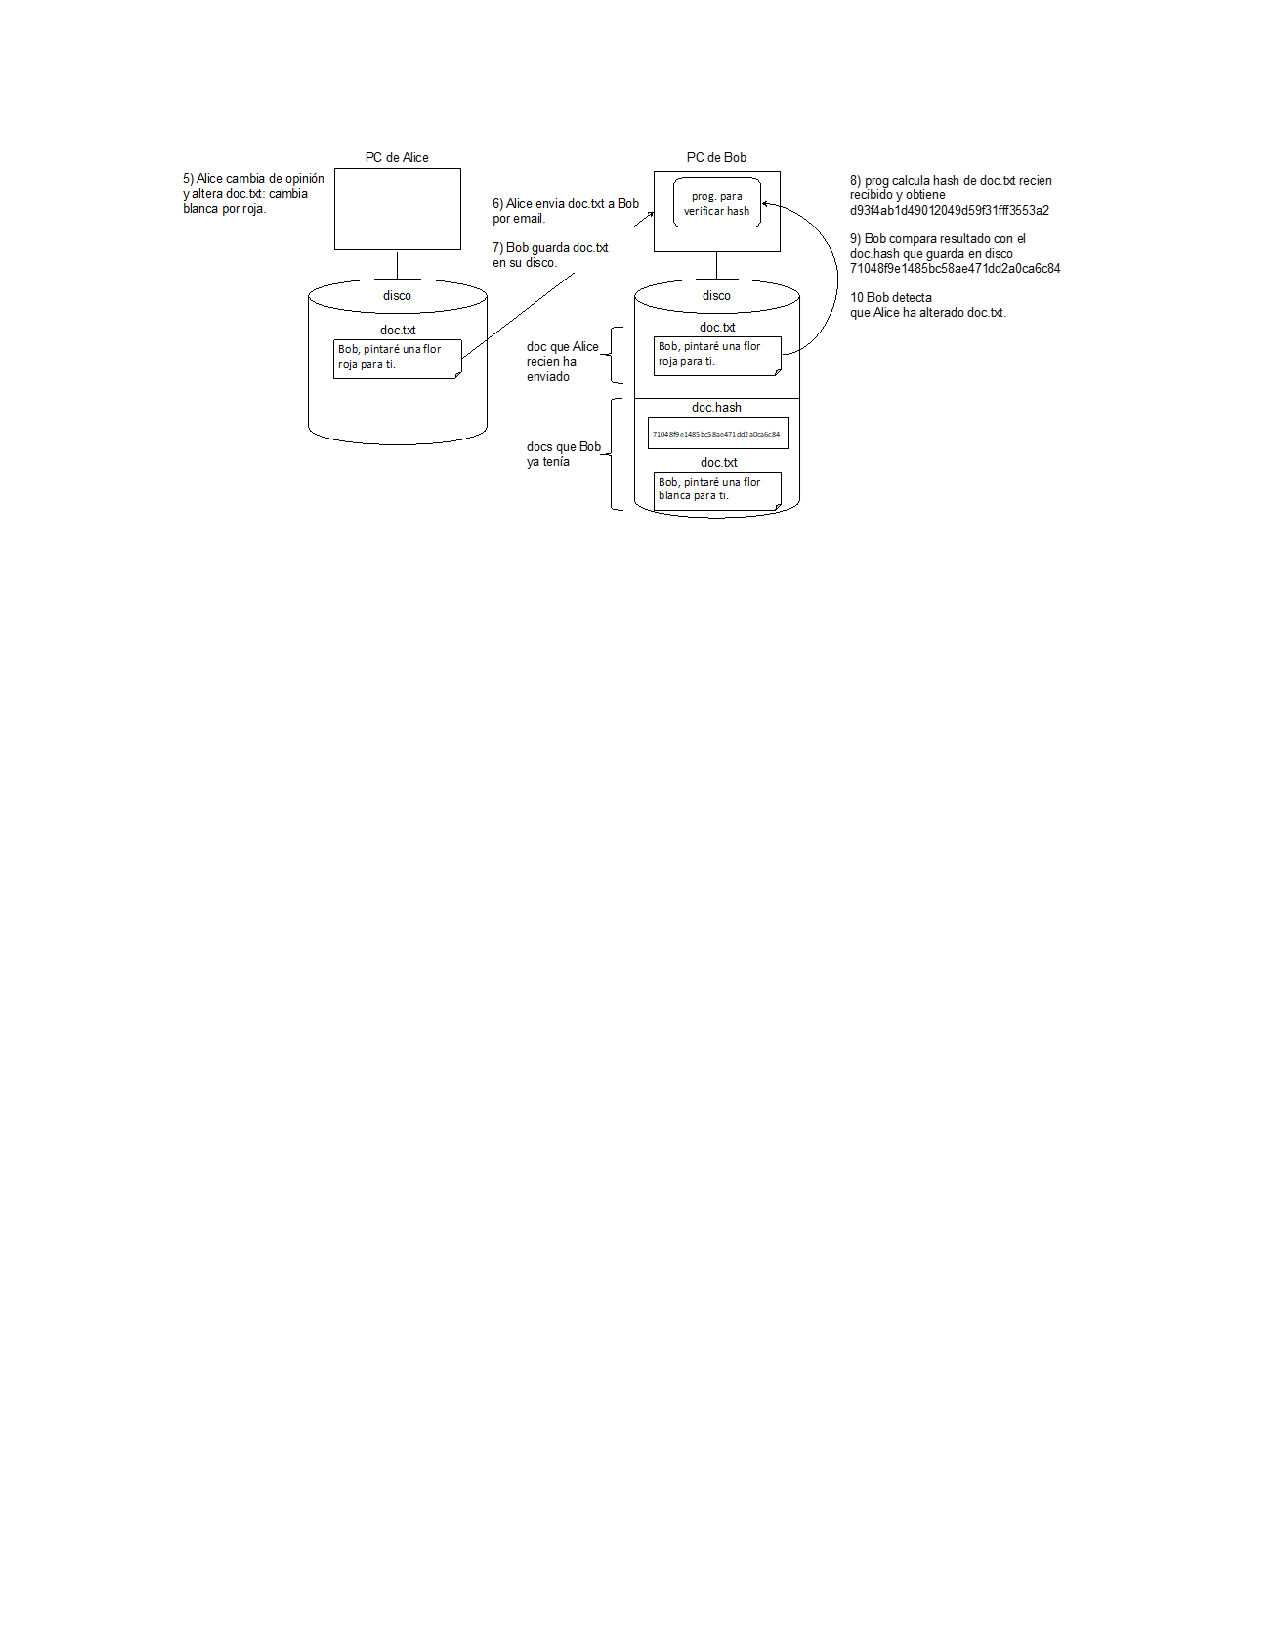
\includegraphics[width=0.85\columnwidth]{imagenes/gatorojo.pdf}
\caption{Concepto de hash}
\label{gatorojo}
\end{figure} 

La Fig.  muestra como Bob se vale de la operación hash para detectar que Alice ha alterado un archivo.

Una herramienta para ocultar información es el “encriptamiento”: La finalidad de encriptar un archivo es que solamente las personas autorizadas puedan comprender el contenido al abrirlo.  Explicaremos el concepto con la ayuda de Alice y Bob, dos usuarios (humanos) de computadoras.

COLOCAR FIGURA

Definimos \textbf{encriptar} como una operación que el dueño de un archivo (por ej Alice) ejecuta sobre ese archivo con el fin de convertir el contenido (por ej, una carta) en una cadena de caracteres cuyo significado es semánticamente ilegible para quien lo abre. El archivo a encriptar se supone que es legible y se conoce como \textbf{archivo texto}.

COLOCAR FIGURA


El “encriptamiento” es una operación criptográfica respaldada por conceptos matemáticos (Teoría de Números) e intuitivamente consiste en cambiar de manera controlada unos caracteres por otros y el orden de dichos caracteres. El resultado de una operación de encriptamiento se conoce como “criptotexto”. El control de la operación se realiza con la ayuda de una llave para encriptar.

Definimos una “llave para encriptar” como un elemento criptográfico que el usuario le proporciona a su programa de encriptamiento para transformar un texto en criptotexto. A nivel técnico, una llave es una cadena de N caracteres. En la práctica N suele ser 32, 64, 128, etc. caracteres. Por el momento representaremos esa llave con la figura de una llave física. El conocimiento de dicha llave permite desencriptar el criptotexto y recuperar el texto original. La Fig. XX explica el procedimiento. Hemos llamado a la llave Ks en donde K viene del inglés key y  es secreta. La línea roja indica que la llave es un elemento crucial para realizar el encriptamiento y desencriptamiento. De esta manera, si Alice perdiera la llave nunca podría recuperar el texto original.
 
COLOCAR FIGURA

Definimos “desencriptar” como la operación que se realiza para convertir, con la ayuda de una llave de desencriptamiento, un criptotexto al texto original. Existen dos tipos de llaves pero por el momento, en el ejemplo utilizado, suponemos que la llave de encriptamiento y desencriptamiento es la misma.
 
COLOCAR FIGURA

\section{Firmas. Concepto}

Para comprender mejor el impacto jurídico de las firmas electrónicas, es importante conocer las diferentes clases de firmas con sustento legal que una persona puede utilizar en distintas circunstancias. 

Las denominaciones “firma electrónica” y “firma digital” que se han utilizado en la práctica del derecho, muchas veces indistintamente, han generado en ocasiones confusiones terminológicas En este capítulo, con el propósito de aclarar los conceptos, las definimos de forma separada y determinamos sus diferencias. Es necesario tener en cuenta que, si bien estas firmas pueden coincidir en varias características; sin embargo, tienen aplicaciones fundamentalmente diferentes, especialmente debido a su naturaleza virtual.

La firma constituye una de las tantas maneras que tiene el derecho para completar la forma de los actos humanos en instrumentos públicos y privados.\footnote{Compagnucci de Caso, Rubén H., “Firma y firma digital”, EBOOK-TR 2021 TOBÍAS, 21/01/2021, 191, Cita Online: AR/DOC/3459/2020.}  Clásicamente estuvo conectada con la idea de la expresión "gráfica" de la voluntad del emisor; pero desde hace uno años perdió relevancia debido a los avances tecnológicos que determinaron el nacimiento de firmas digitales, a la que luego nos referiremos en detalle.

La necesidad de firma persigue diversos fines:

\begin{itemize}
    \item identificar a una persona,
    \item dar certeza sobre la participación personal de esa persona en el acto de firmar
    \item Asociar a esa persona con el contenido de un documento.
    
\end{itemize}

Además, se reconoce que la firma puede desempeñar otras funciones como: demostrar la intención de una parte contractual de obligarse por el contenido del contrato firmado, de reivindicar la autoría de un texto, la intención de una persona de asociarse con el contenido de un documento escrito por otra, o el hecho de que esa persona había estado en un lugar determinado, en un momento dado.

La palabra "firma" se define en el diccionario de la Real Academia Española\footnote{RAE, \url{https://www.rae.es/}}  como "El nombre, apellido o título de una persona que esta pone con rúbrica al pie de un documento escrito de mano propia o ajena para darle autenticidad o para obligarse en lo que en él se dice”, aclarando que "no es solamente escribir el nombre de quien comparece".  De la misma forma, algunos autores como  Guillermo A. Borda\footnote{\cite{Borda1999}} se refieren a la firma como aquella que “normalmente es la manera habitual con la que una persona escribe su nombre con el objeto de asumir las responsabilidades inherentes al documento que suscribe...". A lo que agrega: "Sin embargo el carácter maquinal y la frecuencia de su uso, el deseo del firmante de definir su personalidad o de evitar falsificaciones hacen que, en la frecuencia de su uso la escritura degenere en rasgos en los cuales se hace muy difícil encontrar semejanzas con las letras que componen el verdadero nombre".   Asimismo, Santos Cifuentes afirma que la firma es esencial para dar a conocer el pensamiento y la voluntad del sujeto y luego añade que es el modo habitual que tiene una persona de dar a conocer su individualidad escribiendo su nombre y apellido.\footnote{\cite{Santos1999}“Elementos del Derecho Civil”} 

  Las definiciones de los autores mencionados precedentemente se refieren estrictamente a la firma de puño y letra (hológrafa). Esto se debe al momento temporal en que fueron escritas. Sin embargo, es necesario aclarar que las mismas no se ajustan a la realidad, y se encuentran desactualizadas. Quizás, más apropiado seria decir que es una definición incompleta ya que aluden a una de las clases de firmas (ológrafas). Hoy en día, gracias a la tecnología surgieron otras firmas, como las electrónicas, a las que nos referiremos más adelante. Como bien se expresa a lo largo de esta tesis, el desarrollo tecnológico, más precisamente el surgimiento y auge de la digitalización es el punto de partida de un cambio de paradigma. Además, se convierte en un desafío para los legisladores regular las firmas de forma adecuada. Este capítulo se propone contribuir a aclarar y despejar dudas sobre las distintas clases de firmas que podemos encontrar en el mundo digital.
 
Estas definiciones se utilizarán en otros capítulos como el de contratos, además de mencionarlas en las secciones de esta tesis donde se requiera.

\section{Firmas hológrafas}

El vocablo "hológrafo" significa escrito de mano del autor, autógrafo, sin indicación del soporte en el cual se realiza la escritura.

Por su parte, si nos remitimos al CCyC en el art. 288 establece que. “.... Debe consistir en el nombre del firmante o en un signo”. 

Las firmas manuscritas en documentos en papel se han utilizado durante mucho tiempo como prueba de autoría ya que tienen las siguientes propiedades:

\begin{itemize}
    \item Es difícil de falsificar. El proceso de generar una firma es un "reflejo entrenado", que no está sujeto al control mental consciente. Por tanto, la imitación de las firmas es difícil, especialmente a una velocidad de escritura normal; esto explica por qué los empleados bancarios a menudo piden que se firmen documentos mientras están mirando.\footnote{Jianying Zhou, Robert Deng, “On the Validity of Digital Signatures”, ACM SIGCOMM Computer Communication Review, volumen 30, 2, abril, 2000} 
    \item Es fácilmente verificable. La técnica de verificación tradicional se basa en la inspección visual de una firma escrita. Sin embargo, la verificación puede resultar difícil para las personas que son muy inconsistentes con sus firmas.
    \item No es reutilizable. La firma es parte del documento. Otras personas no pueden cortar y pegar la firma en otros documentos.
    \item El documento firmado es inalterable. Sin embargo, existe una limitación. La firma en un documento solo puede garantizar el origen y la integridad de la hoja única del documento que lleva la firma. Por lo tanto, para garantizar el origen y la integridad de todo un documento legal, debe firmarse en cada hoja. 

\end{itemize}

La firma de un documento es un objeto físico que puede presentarse para la resolución de disputas. Es una prueba de no repudio. Para que una firma recién generada sea aceptable, debe compararse con una muestra notariada como la firma de una tarjeta de crédito. Para hacer cumplir el no repudio y simplificar la resolución de dis	Firmas electrónicasputas, un tercero (de confianza) puede presenciar la firma de un documento (escribano) [2].

\section{	Firmas electrónicas}

Definimos a la \textbf{firma electrónica} como datos electrónicos (S) directamente anexados o lógicamente asociados a otros datos (D) con el fin de vincular jurídicamente al firmante con lo estipulado en los datos D.

Para facilitar la explicación del concepto de firma electrónica, es oportuno convenir a D como un documento (posiblemente de varias páginas), por ejemplo, un documento electrónico guardado en disco. Supongamos que el firmante es Bob y que Alice es la emisora de D. Bob y Alice podrían ser personas físicas o jurídicas. D es uno o más documentos que estipulan una o más cláusulas que Bob acepta para beneficio de Alice, al estampar su firma S. En la práctica, D contiene también cláusulas a las que Alice queda jurídicamente vinculada si Bob firma.

Según Ross Anderson\footnote{\cite{Andersson2020}“Security Engineering”} , una firma electrónica es un mecanismo jurídico que se usa en procedimientos legales y que debe cumplir con varios requisitos:

\textbf{Vinculación:} S está unido al firmante Bob y por ende, D queda vinculado al firmante cuando éste estampa su firma en D. Después de firmar, Bob ya no puede retractarse sin tener consecuencias legales.

\textbf{Identificación:} Se identifica al firmante.

\textbf{Control:} La tecnología para crear S esta bajo el control del firmante.

\textbf{Integridad:} después que Bob estampa su firma S en D, D queda sellado, ni Bob, ni Alice ni nadie puede modificar D sin que Bob pueda detectarlo.
 	
Como lo muestra la Fig. FF, existen varias tecnologías que se pueden usar para estampar una firma electrónica. La figura solo muestra las más conocidas actualmente, hay otras que no hemos mencionado, otras que han caído en desuso y otras que podrían aparecer en el futuro. Para colocar la figura dentro del contexto, mencionamos también las firmas holográficas.

Esta figura \ref{Fig. Clases de firmas holografica y electronica}

\begin{figure}
\centering
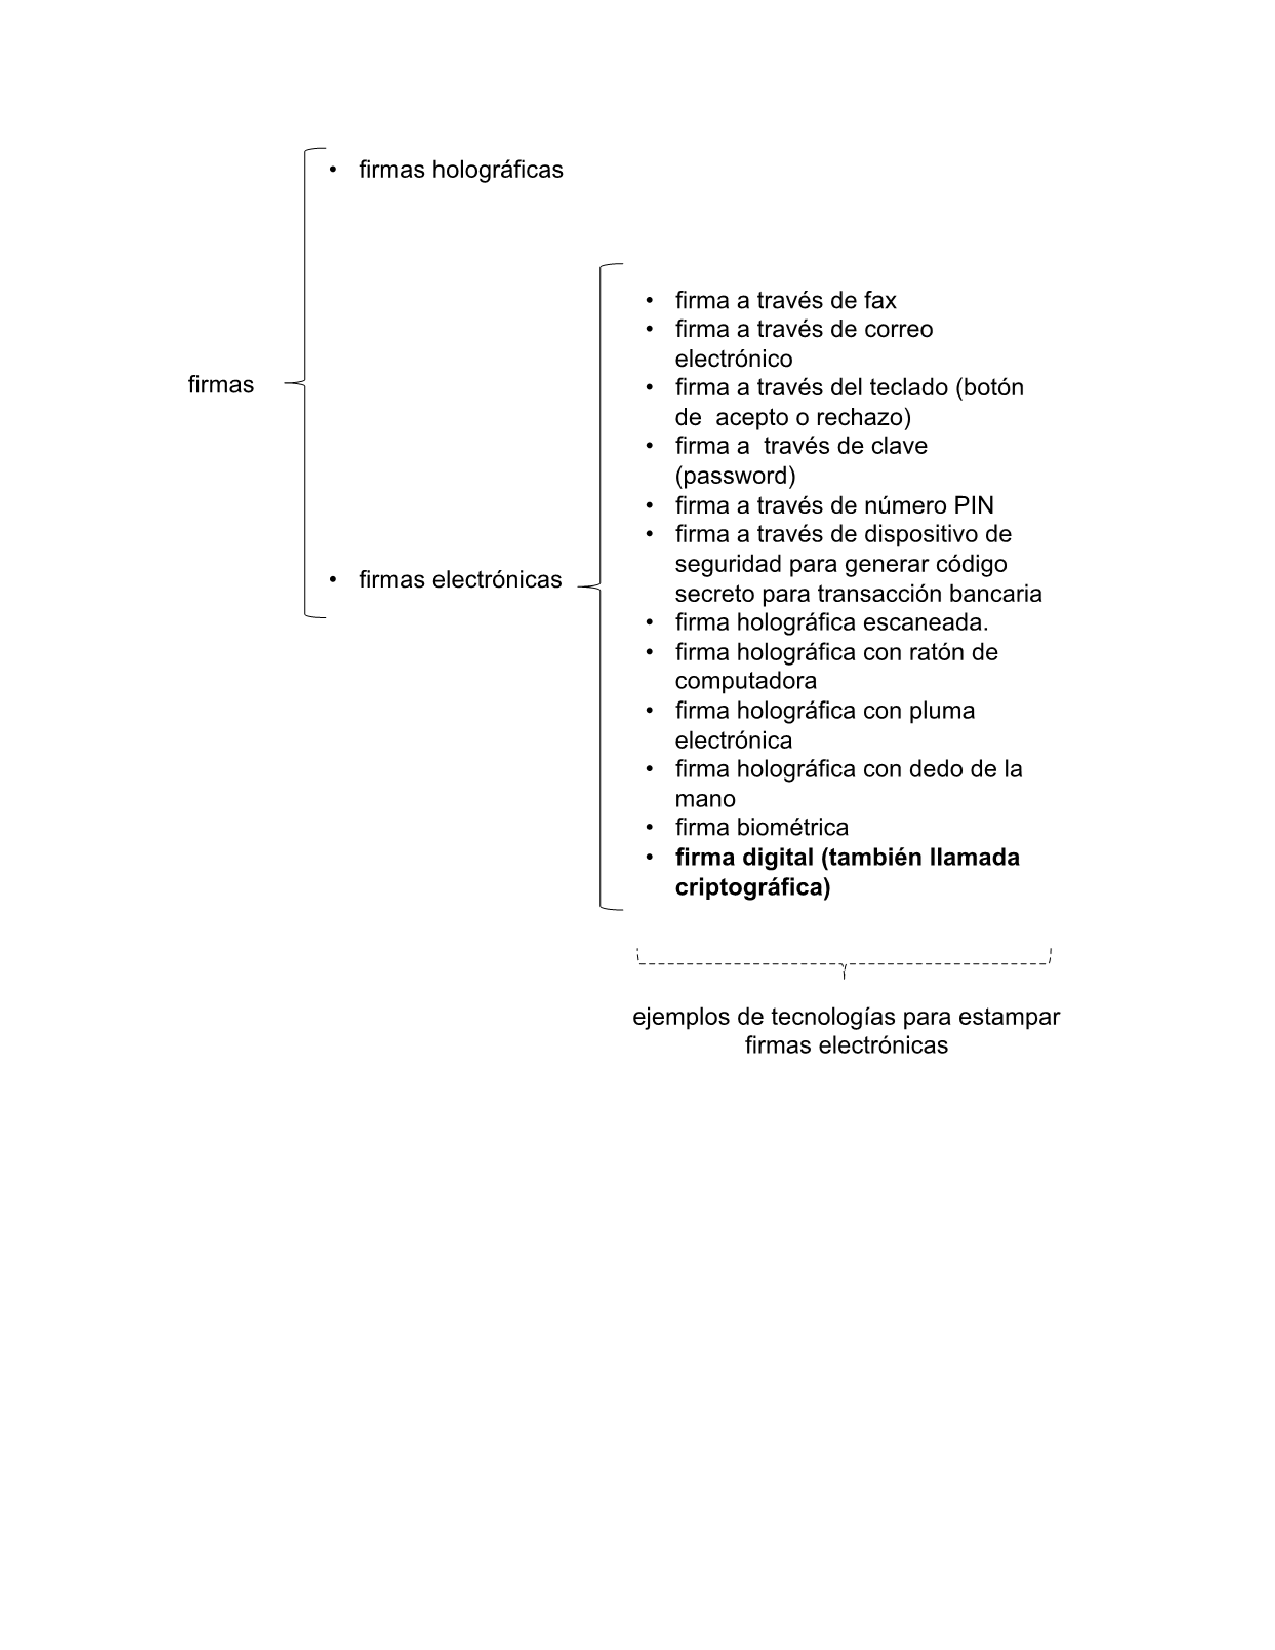
\includegraphics[width=0.85\columnwidth]{imagenes/clasesfirmashologyelectro.pdf}
\caption{Clasificación de firmas desde el punto de vista de la tecnología empleada}
\label{Fig. Clases de firmas holografica y electronica}
\end{figure} 

La tecnología utilizada determina hasta qué grado una firma electrónica puede garantizar los requisitos antes mencionados. Algunas son más vulnerables que otras; también determina el costo y la complejidad. En la figura, hemos colocado con letras negritas las firmas digitales porque son parte central de esta tesis. De hecho, las explicamos detenidamente en la Sección XXX. De acuerdo con la figura, una firma digital es una clase de firma electrónica basada en tecnología criptográfica que usa llaves públicas y privadas. Esta tecnología se sustenta en la Teoría de Números y, específicamente, en el conocimiento de algunas operaciones que no las pueden realizar rápidamente ni las super-computadotras más veloces. Por ejemplo, de la Teoría de Números se sabe que es muy sencillo calcular el producto de dos números primos grandes (digamos que de 1024 bits como en el RSA estándar), por ejemplo (p)(q)= r.  Sin embargo, la operación opuesta (factorizar el número r que resulta de la multiplicación) en los dos factores p y q, es complicada, a tal grado que la supercomputadora más potente tardaría miles de años en realizarla.

Un ejemplo de un número primo de 1024 bits es:

Un ejemplo de un número primo de 1024 bits es:

Para darle mayor claridad a nuestra explicación, mostramos en las Figuras YY a ZZ algunos ejemplos prácticos de firmas electrónicas: fax, email, entre otras. 

Esta figura \ref{Fig. Firmaemail}


\begin{figure}
\centering
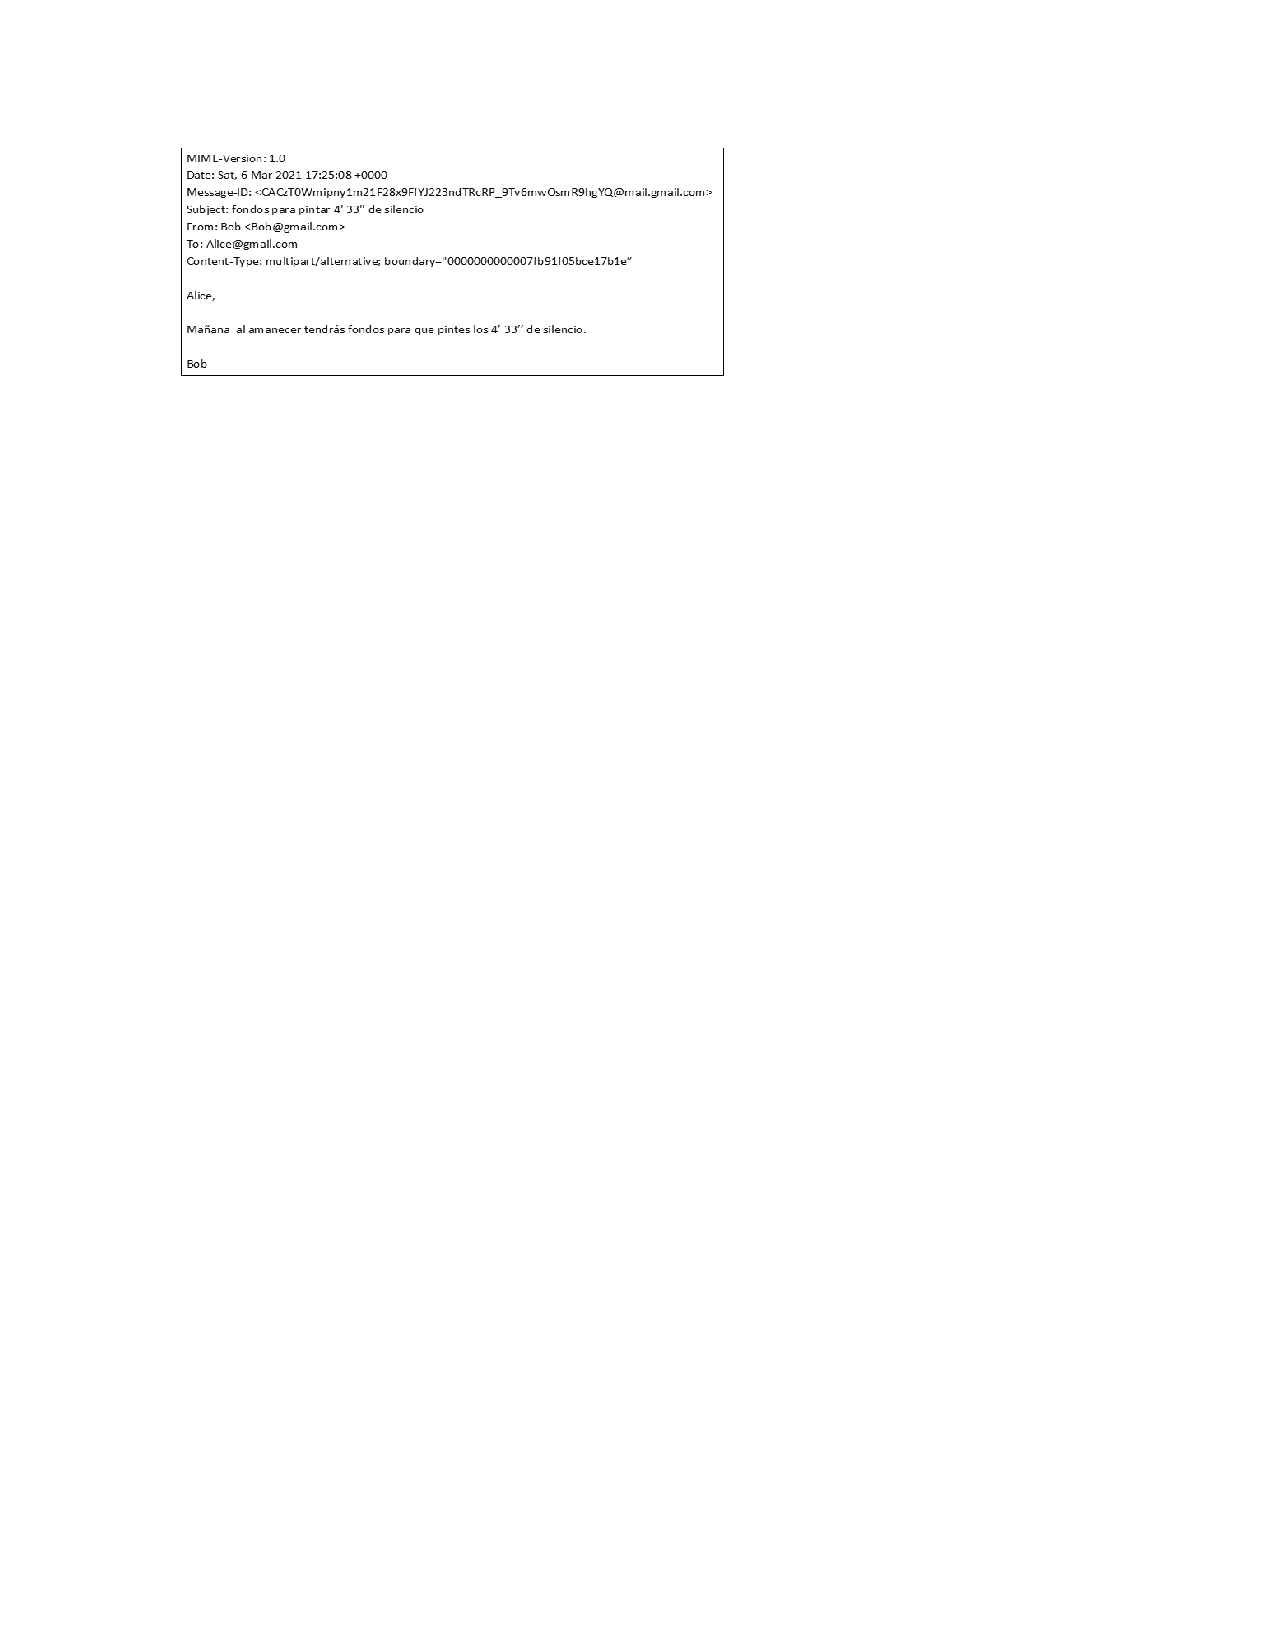
\includegraphics[width=0.85\columnwidth]{imagenes/firmaemail.pdf}
\caption{Ejemplo de firma a través de email.}
\label{Fig. Firmaemail}
\end{figure} 


\begin{figure}
\centering
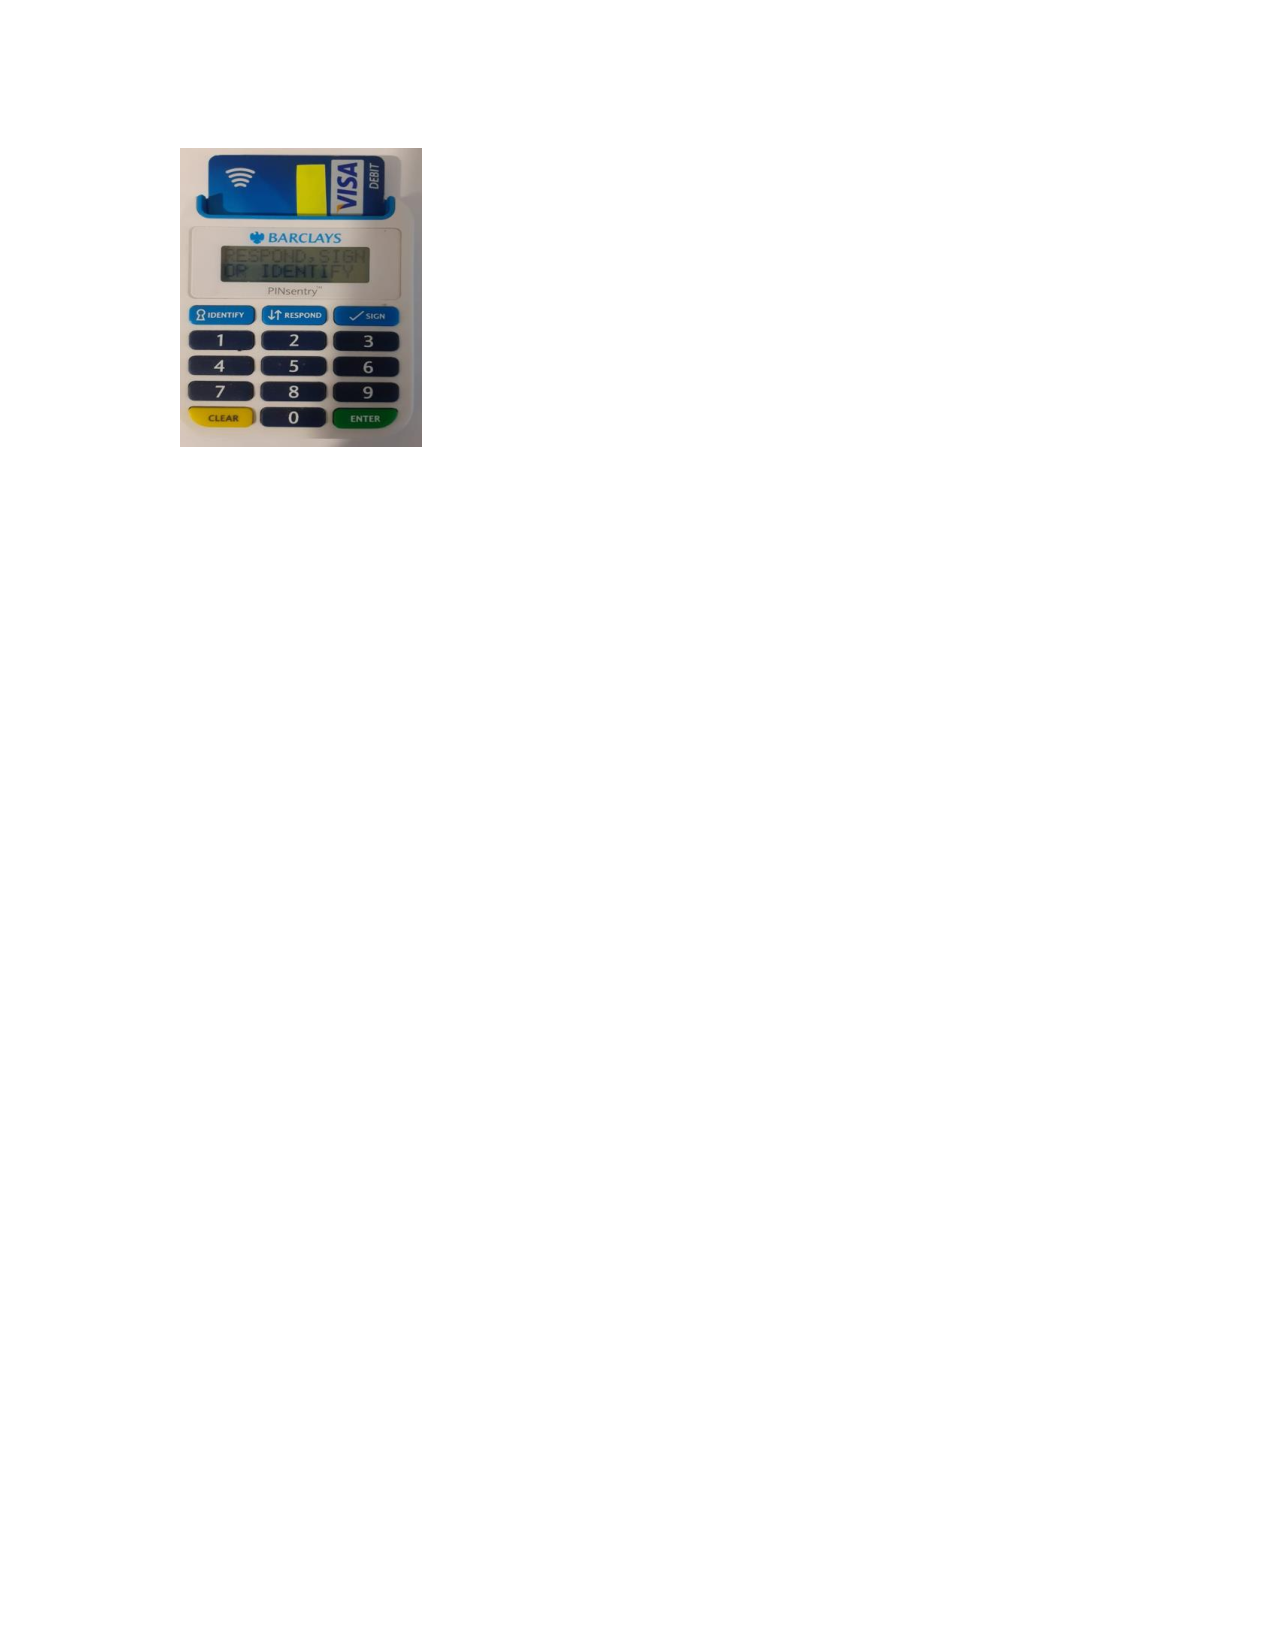
\includegraphics[width=0.85\columnwidth]{imagenes/firmadispositivo.pdf}
\caption{Ejemplo de firma a través de dispositivo de seguridad.}
\label{Fig. Firmadispositivo}
\end{figure} 

Esta figura \ref{Fig. Firmaclickwrap}

\begin{figure}
\centering
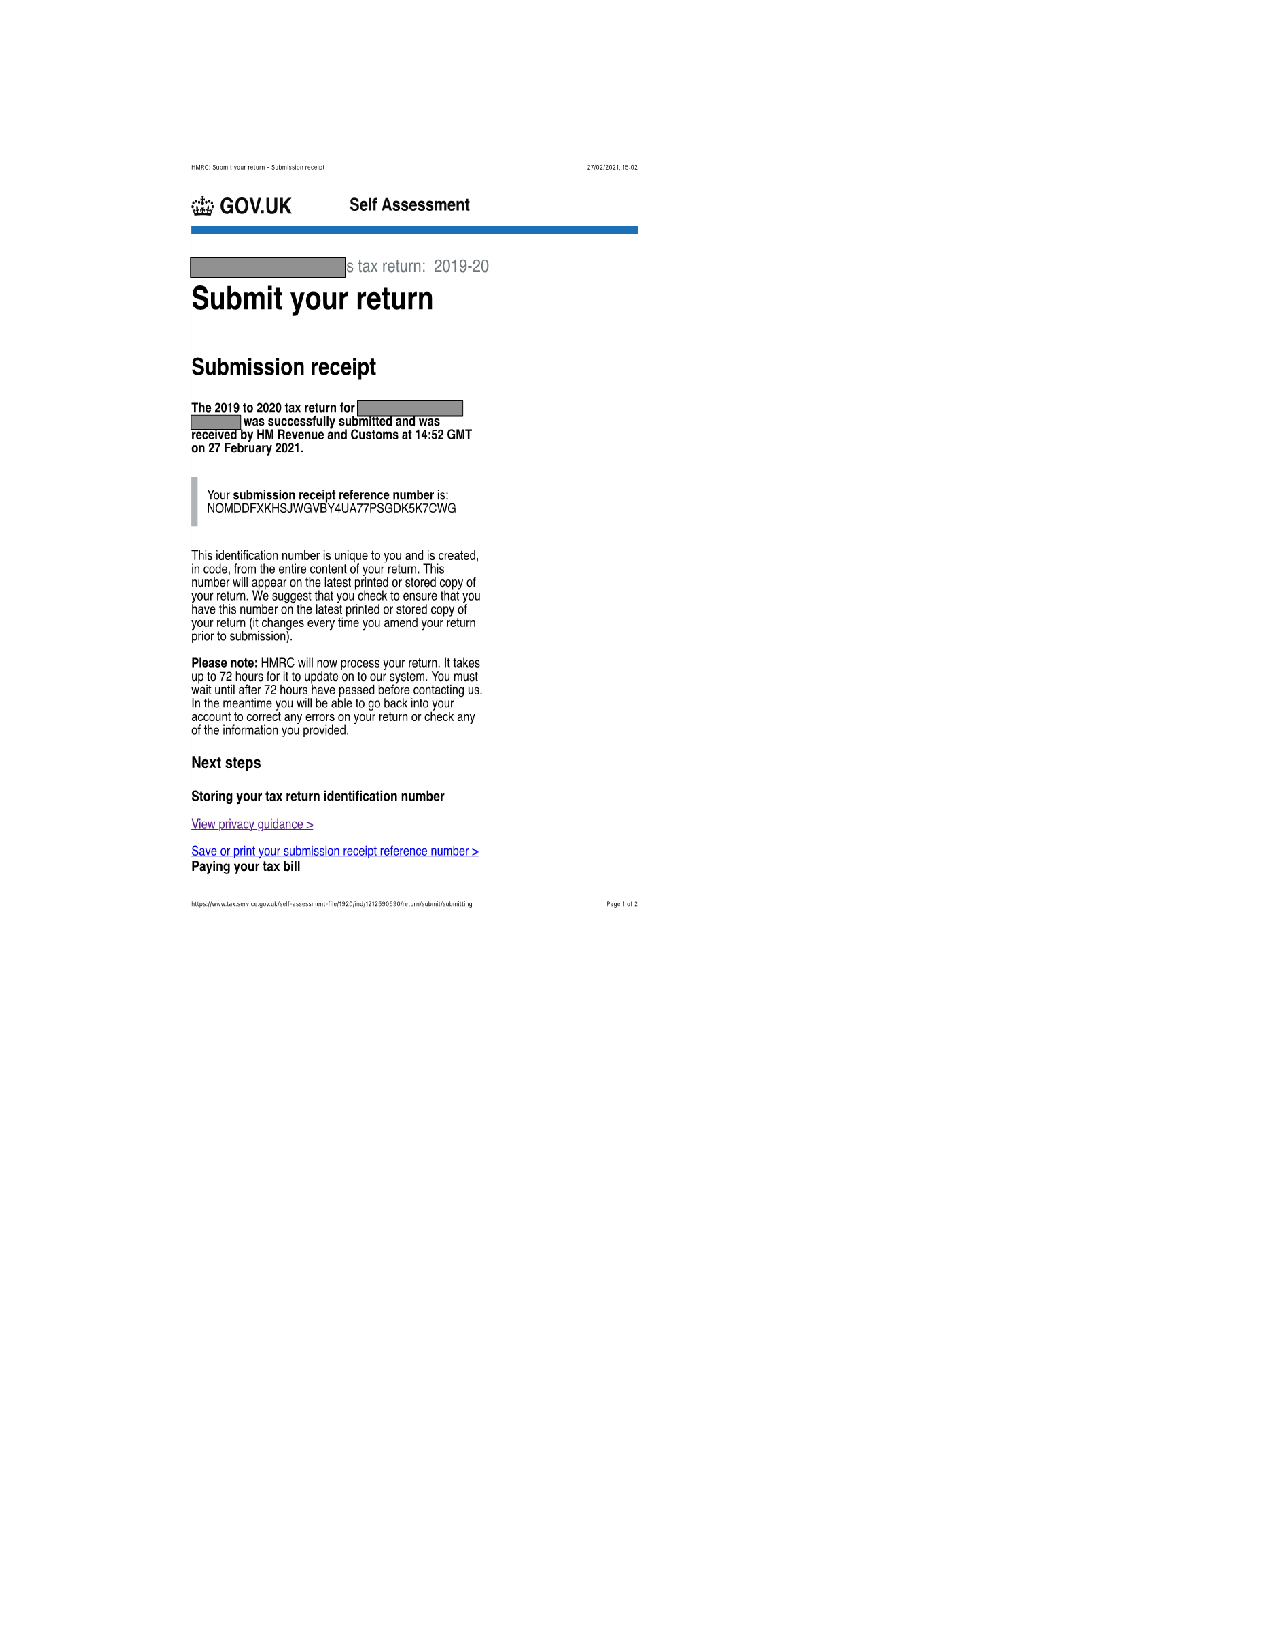
\includegraphics[width=0.85\columnwidth]{imagenes/firmaclickwrap.pdf}
\caption{Ejemplo de firma a través del botón de aceptar o rechazar.}
\label{Fig. Firmaclickwrap}
\end{figure} 

\textbf{Encriptamiento basado en llaves públicas y privadas (public-private key encryption):} es una técnica criptográfica que se puede usar para encriptar documentos utilizando dos llaves: una llave pública y una llave privada. Fue propuesta en 1976 por Deffie y Hellman.

En la tecnología de llave pública-privada, una de las llaves se utiliza para encriptar y la otra para desencriptar. Se cataloga como una técnica asimétrica porque las llaves para encriptar y desencriptar son diferentes. La Fig XX ilustra el concepto.

Esta figura \ref{Fig. llavespublicaprivada}

\begin{figure}
\centering
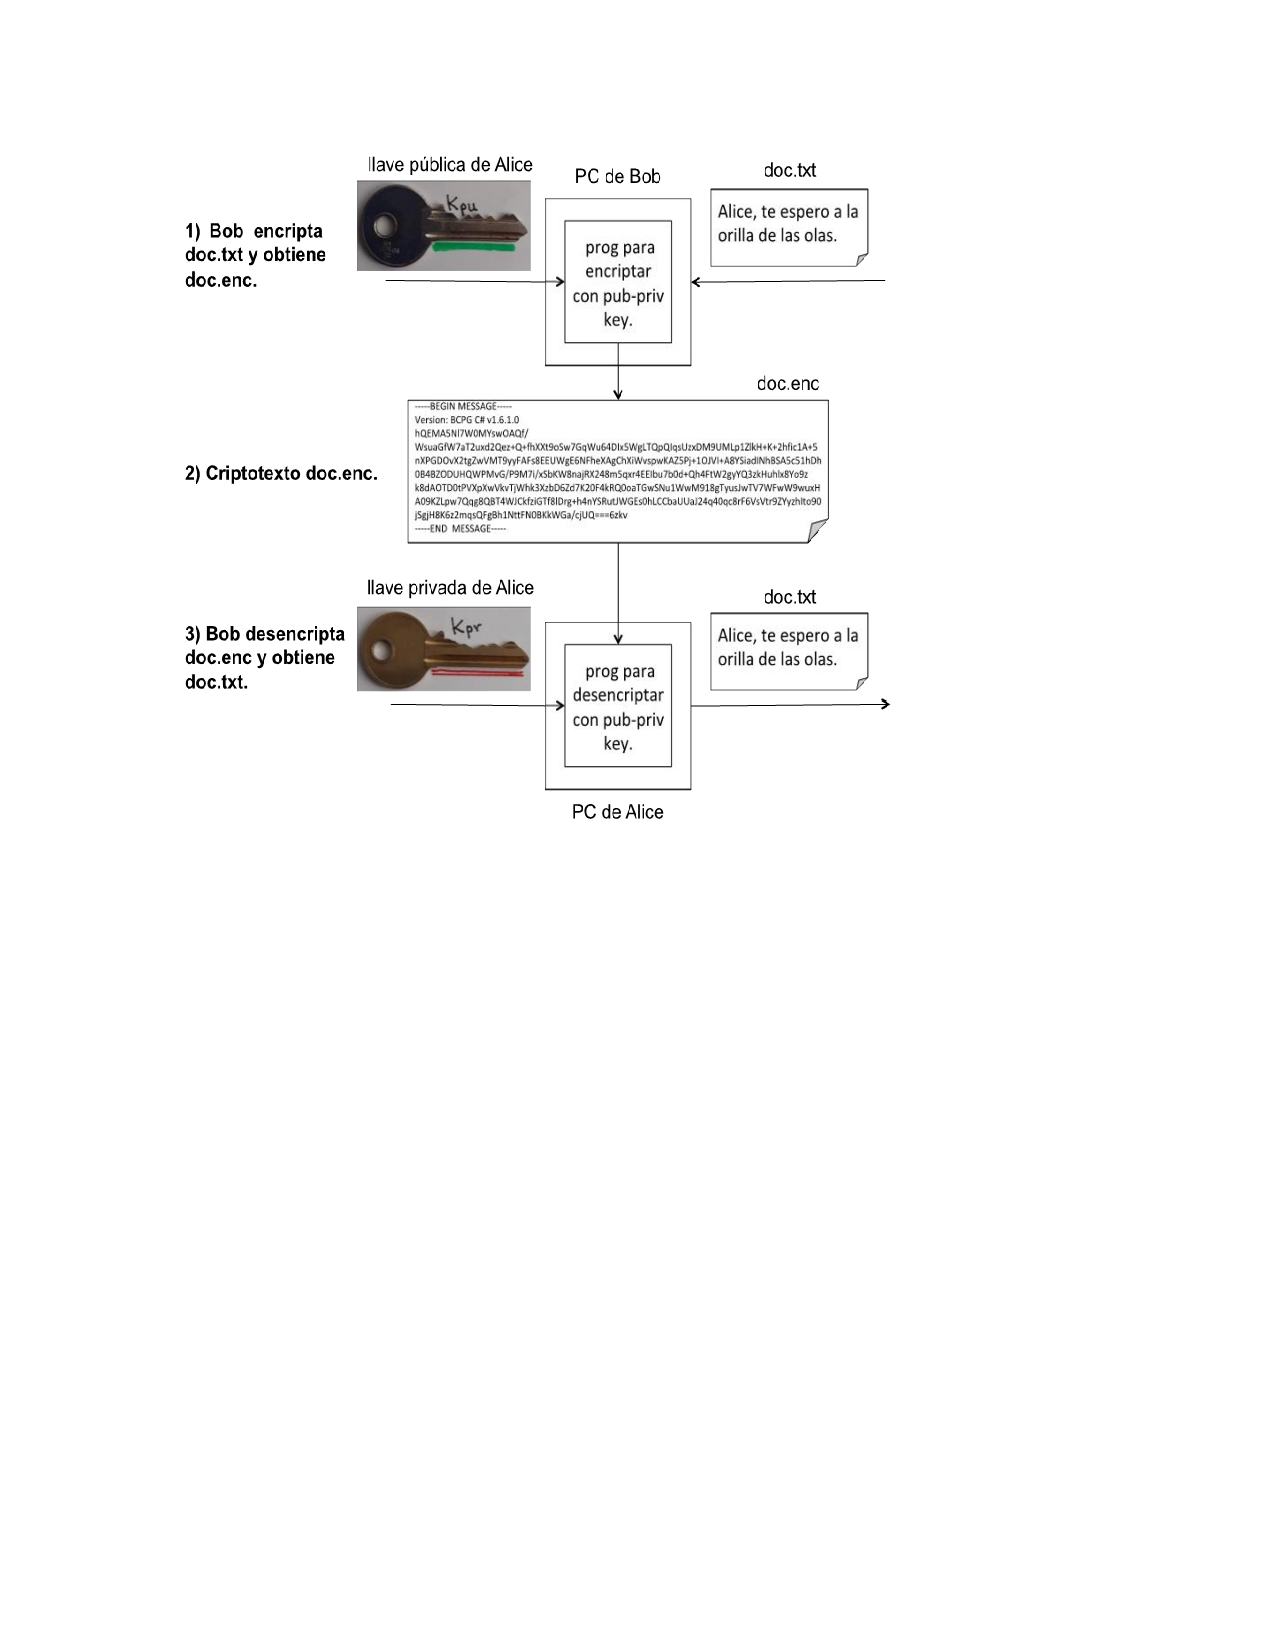
\includegraphics[width=0.85\columnwidth]{imagenes/llavespublicaprivada.pdf}
\caption{Ejemplo de firma a través llave publica privada.}
\label{Fig. llavespublicaprivada}
\end{figure} 

\textbf{Pares de llaves públicas y privadas:} son dos llaves criptográficas asociadas criptográficamente (en otras palabras, matemáticamente): una es la llave pública y la otra es la llave privada. Se pueden realizar con un programa generador de llaves, siempre por pares; cada par es único. Por ejemplo: el par Kpu\_alice y Ppr\_alice es único y asocia Kpu\_alice a Kpr\_alice. Similarmente el par Kpu\_bob y Ppr\_bob es único y asocia Kpu\_bob a Kpr\_bob.

Lo que encripta una llave privada lo desencripta la llave pública correspondiente y al revés, lo que encripta una llave pública, lo puede desencriptar la llave privada par. Por ejemplo, lo que encripta Kpu\_alice, lo puede desencriptar Kpr\_alice y al revés, lo que encripta Kpr\_alice, lo puede desencriptar K\_pu\_alice.  Sin embargo, lo que encripta K\_pr\_alice no lo puede desencriptar K\_pr\_bob. Las llaves trabajan exclusivamente con sus pares, no con otros.

\textbf{Llave pública:} Es una cadena de caracteres que se utiliza dentro de la criptografía de llave pública-privada. Se puede usar para encriptar y para desencriptar.  Lo que encripta una llave privada lo desencripta la llave pública correspondiente y al revés, lo que encripta una llave pública, lo puede desencriptar la llave privada par.  Se llama llave pública porque el propietario se la entrega a las persona o personas con las que espera intercambiar mensajes. Incluso el dueño la puede colocar en un sitio público, como una web page o una red social. En las figuras, que usamos en este trabajo las llaves públicas se encuentran señaladas con una línea de color verde para sugerir que no es una llave que el propietario debe ocultar.

La fig XX muestra un ejemplo \ref{Fig. llavepublica}

\begin{figure}
\centering
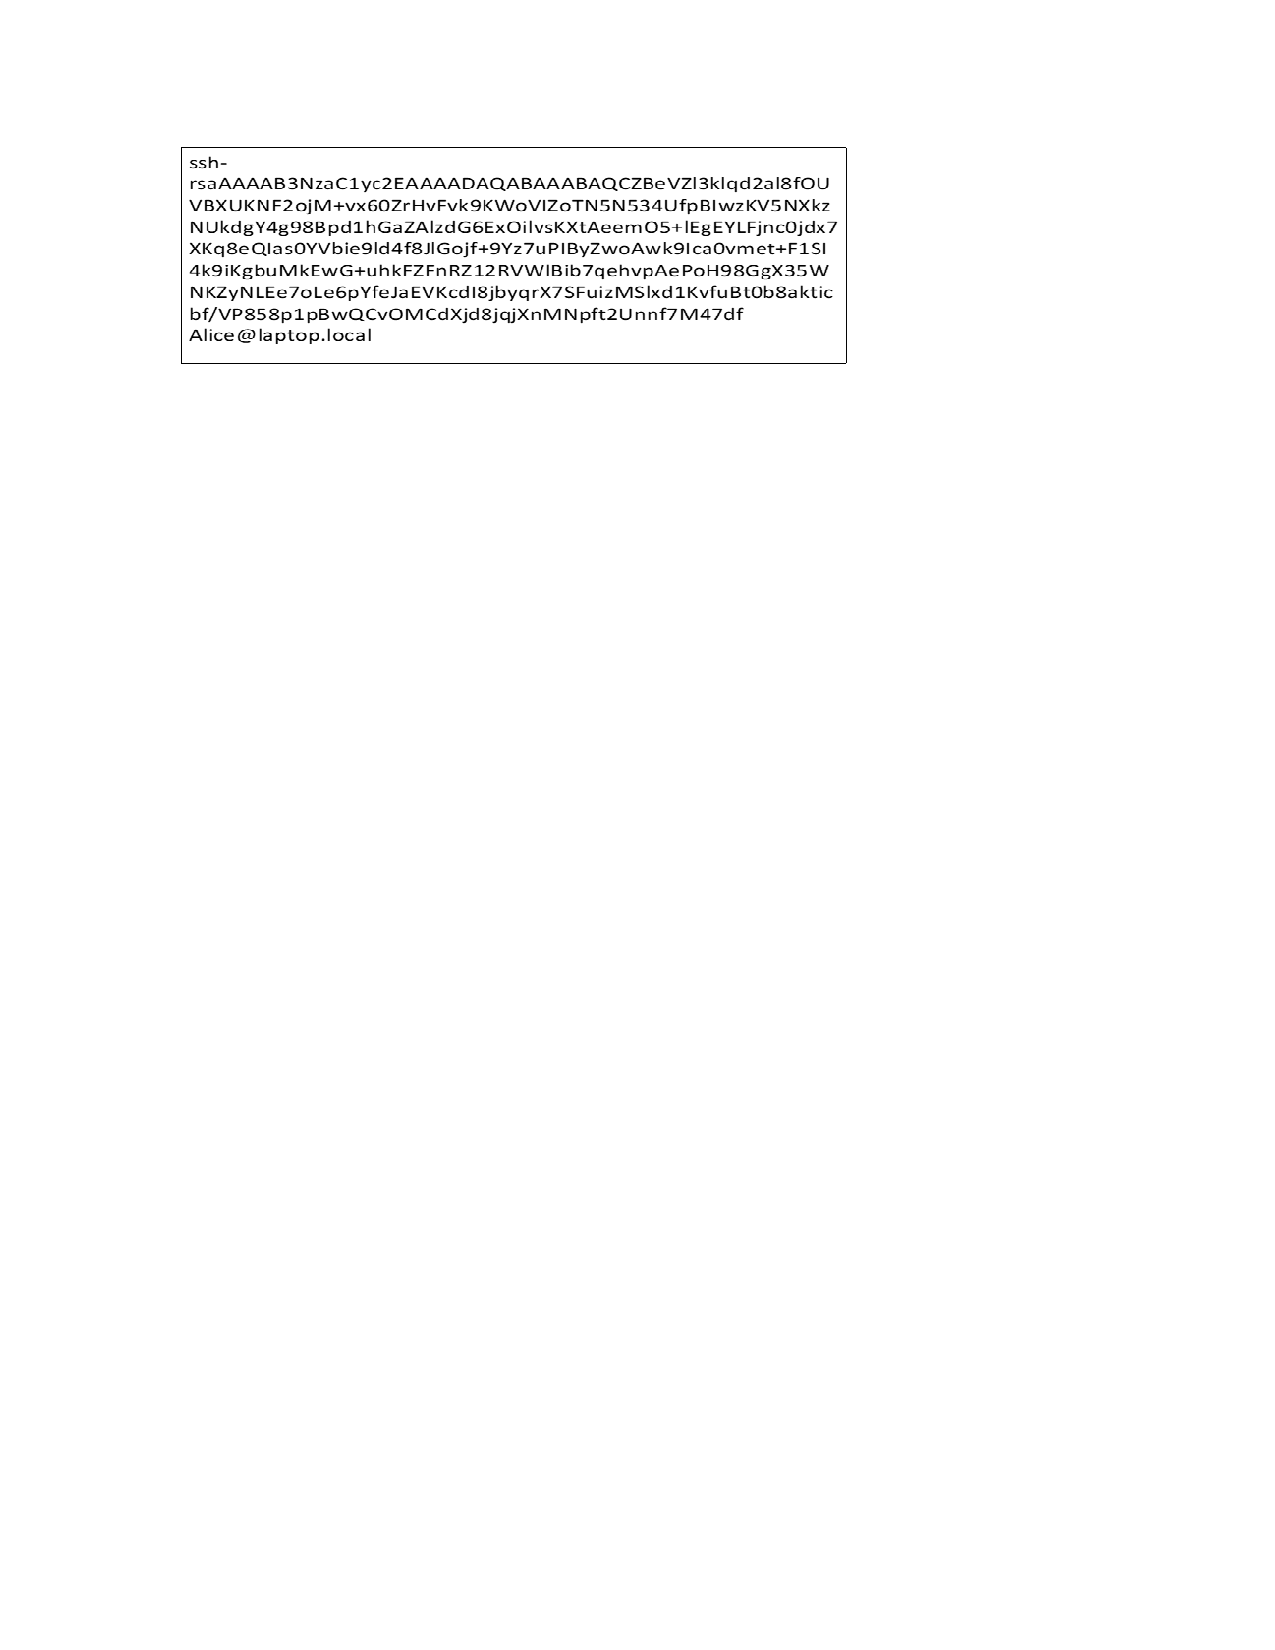
\includegraphics[width=0.85\columnwidth]{imagenes/figllavepublica.pdf}
\caption{Ejemplo de llave pública de Alice.}
\label{Fig. llavepublica}
\end{figure} 

\textbf{Llave privada:} Es una cadena de caracteres que se utiliza dentro de la criptografía de llave pública-privada. Se puede usar para encriptar y para desencriptar. Lo que encripta una llave privada lo desencripta la llave pública correspondiente y al revés, lo que encripta una llave pública, lo puede desencriptar la llave privada par. Se llama llave privada porque el propietario debe mantenerla en privado, es decir, no mostrársela a nadie, ni siquiera a la persona o personas con las que espera intercambiar mensajes. A dichas personas, el propietario les entrega la llave pública correspondiente. Sin embargo, es recomendable que el dueño la guarde en el disco de su computadora, si ésta es exclusivamente para uso personal o, mejor aún, en algún dispositivo que sea separable de su computadora como una memoria USB. En las figuras, que usamos en este trabajo, las llaves públicas se encuentran marcadas con una línea de color rojo para sugerir la importancia de mantener esta llave fuera del alcance de otras personas.

\section{Infraestructura tecnológica para encriptamiento con llaves públicas y privadas y certificados}

Esta tecnología está pensada para uso remoto, es decir, para que personas que solamente se conocen las usen; por ejemplo, que Bob que vive en Florencia y trabaja en la Universidad de Florencia, pueda encriptar un mensaje para Alice que vive en Rosario. De aquí surge uno de los problemas más importante a resolver: Alice necesita estar segura de que el mensaje que ha recibido encriptado con una firma privada, lo ha enviado Bob, el Bob que ella conoce virtualmente. La solución es la certificación de la llave de Bob, una de las áreas que resuelven las llamadas infraestructuras para llaves públicas-privadas \textit{(Public Key Infrastructure- PKI)}, a través de certificados expedidos por las autoridades certificadoras (CA) \textit{(Root Certification Authorities)}.

Una infraestructura PKI  es una combinación de  empresas y equipo de software y hardware destinado al manejo de las llaves pub-key. El manejo incluye la expedición y revocación de certificados. Las empresas que juegan un papel fundamental son las autoridades certificadoras.

Las autoridades certificadoras son empresas que han sido aprobadas por los gobiernos para expedir certificados. Existen alrededor de XX \textit{Root Certification Authorities}, actualmente las más conocidas son: Symantec,  RapidSSL,  GeoTrust, DigiCert, VeriSign.\footnote{\url{https://ccadb-ublic.secure.force.com/microsoft/IncludedCACertificateReportForMSFT}}

El precio de un certificado varía, dependiendo de la autoridad que lo venda y del alcance del certificado (la seguridad de las llaves, número de browser que aceptan el certificado, etc.). Actualmente todos los certificados tienen una validez de un año. \footnote{\url{ https://aboutssl.org/the-worlds-most-trusted-ssl-brands/}}

Un certificado de una llave pública (public key certificate) es un documento digital expedido y firmado oficialmente por una autoridad certificadora que avala que una llave pública pertenece a una empresa o persona.  Dicho de manera simple, el certificado de Bob es la llave pública de Bob firmada (avalada) por una autoridad reconocida como una autoridad al menos por Alice, la receptora del mensaje de Bob.

Los campos más importantes que un certificado contiene son:

\begin{itemize}
    \item la fecha de inicio de vigencia: 30 Dic 2020
    \item el tiempo de vigencia: actualmente se expiden por 12 meses.
    \item el tiempo de vigencia: actualmente se expiden por 12 meses.
    \item la llave pública que el certificado avala
\end{itemize}

 Nota: en la práctica un certificado puede contener varias llaves públicas, en lugar de solamente una.

Al firmar la CA declara que ha verificado la información contenida en el certificado (como nombre de Bob, dirección, teléfono, etc.) y en la información adicional que queda guardada en su base de datos. 

Al recibir el mensaje de Bob, un programa de su computadora verifica automáticamente que la firma de Bob está respaldada por un certificado de una CA, cuya firma Alice reconoce.

\textbf{Cadena de certificados:} en la práctica los certificados están validados por una estructura jerárquica en donde existen empresas conocidas como \textit{Root Certification Authorities} que expiden certificados a empresas de segundo nivel y estas a otras empresas de tercer nivel y así hasta llegar a las empresas como universidades o bancos que expiden certificados a sus empleados. \footnote{\url{https://www.checktls.com/showcas.html}}

De esta manera, el certificado de Bob puede no estar firmado por una firma que Alice reconoce, sino por otra que es desconocida para Alice pero que su software puede seguir al ascender por la estructura jerárquica verificando firmas hasta llegar a una firma que su software reconoce como válida, posiblemente hasta llegar a alguna de las CA.

Para ganar en velocidad, los browsers de las computadoras y de los teléfonos móviles,  almacenan al momento de instalarlos, varios de los certificados mas populares:

Esta figura \ref{Fig.certificadofirma}


\begin{figure}
\centering
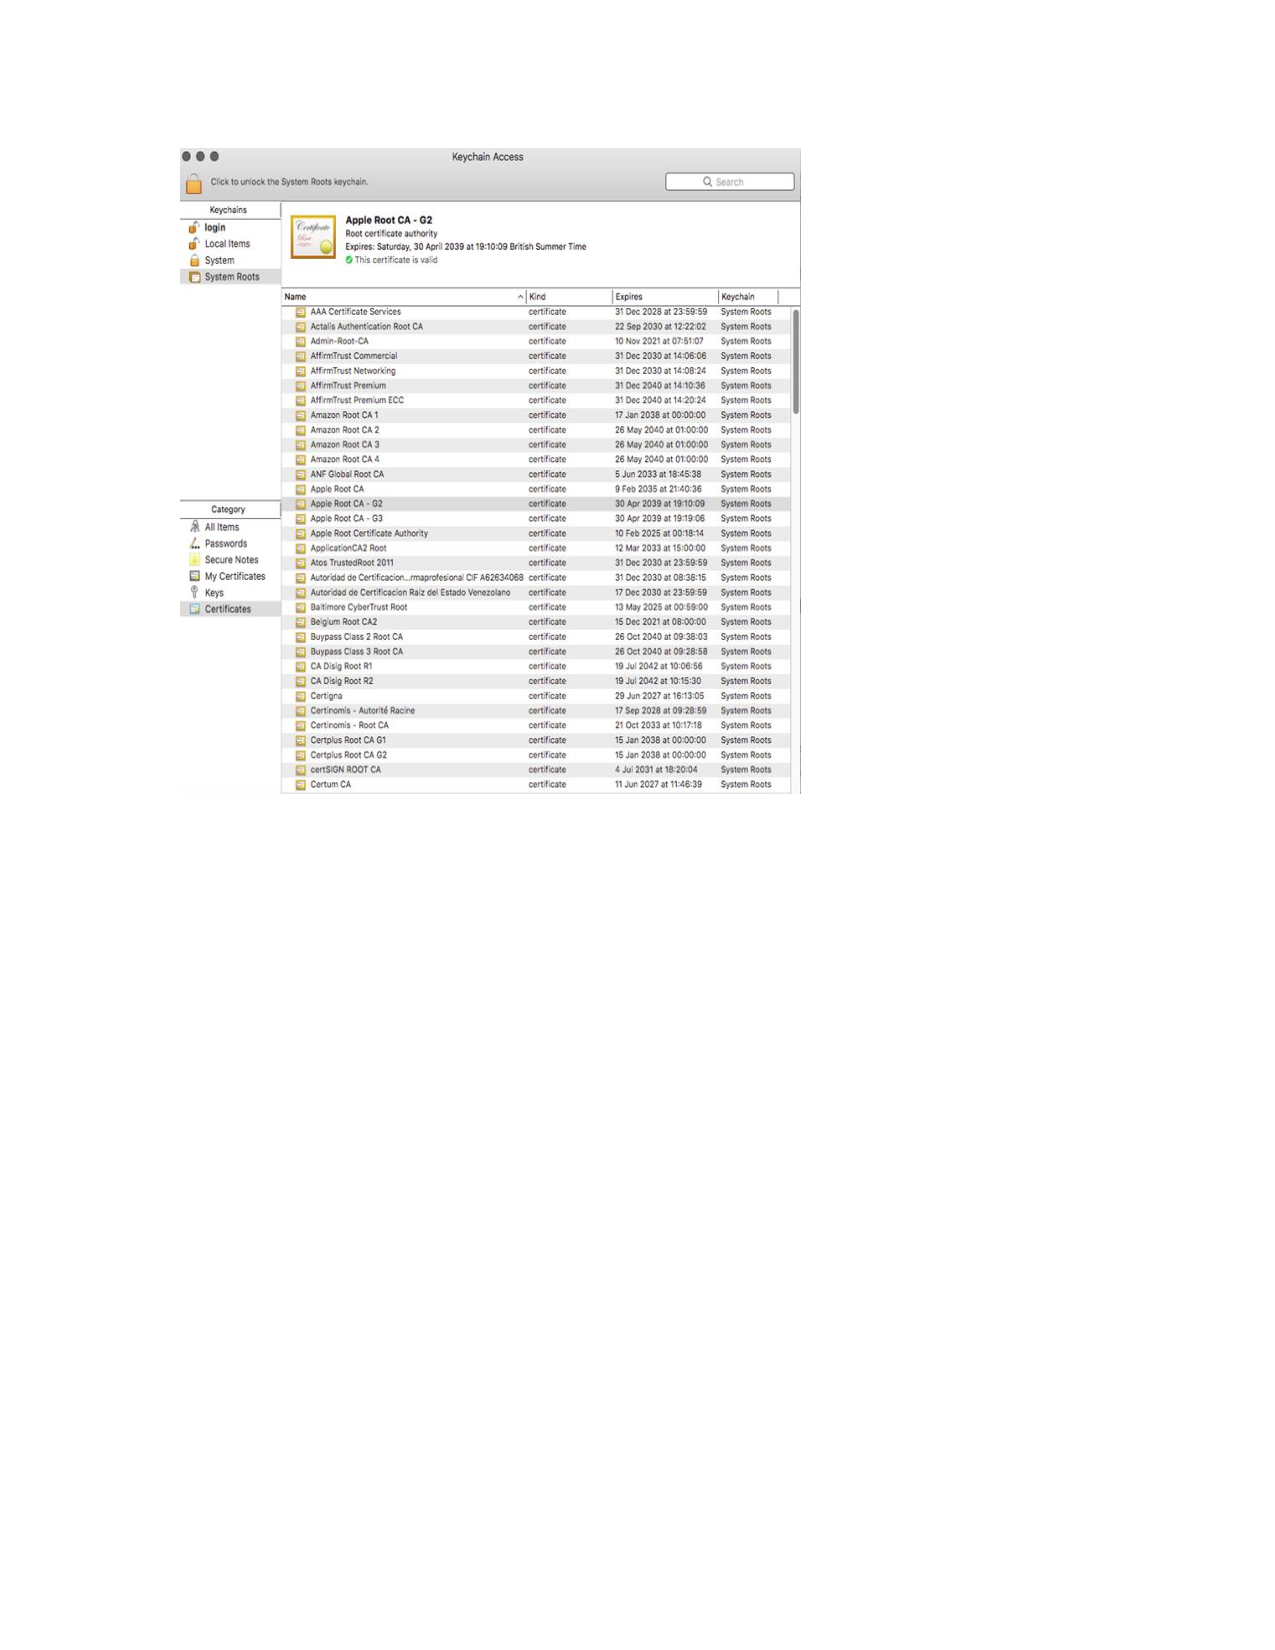
\includegraphics[width=0.85\columnwidth]{imagenes/certificadofirmaej.pdf}
\caption{ejemplo de certificados almacenados en una laptop Mac (1)}
\label{Fig.certificadofirma}
\end{figure} 

Esta figura \ref{Fig.ejemploclmacenamientodecertificadodefirma}

\begin{figure}
\centering
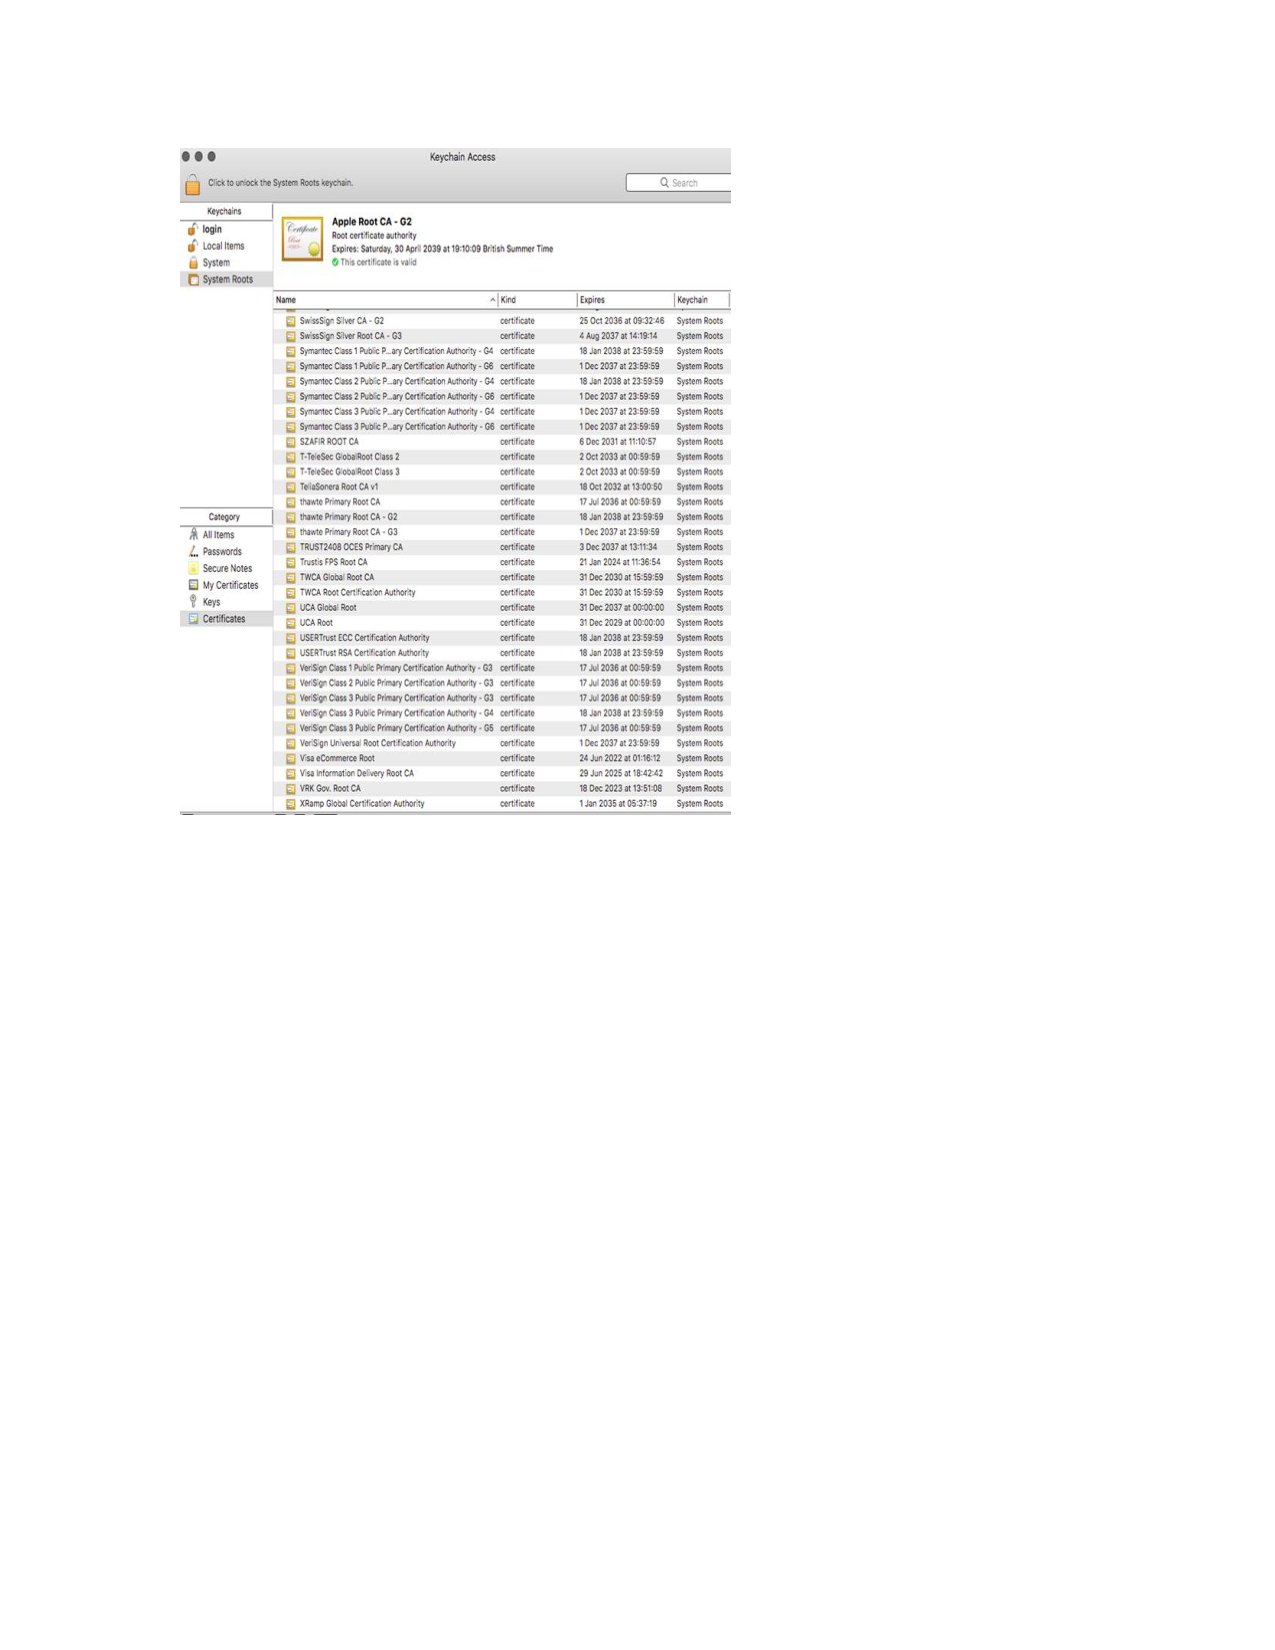
\includegraphics[width=0.85\columnwidth]{imagenes/otroejcertalmacenadoenlaptop.pdf}
\caption{ejemplo de certificados almacenados en una laptop Mac (2)}
\label{Fig.ejemploclmacenamientodecertificadodefirma}
\end{figure} 

Esta figura \ref{Fig.ejemplocertificadoVerisign}

\begin{figure}
\centering
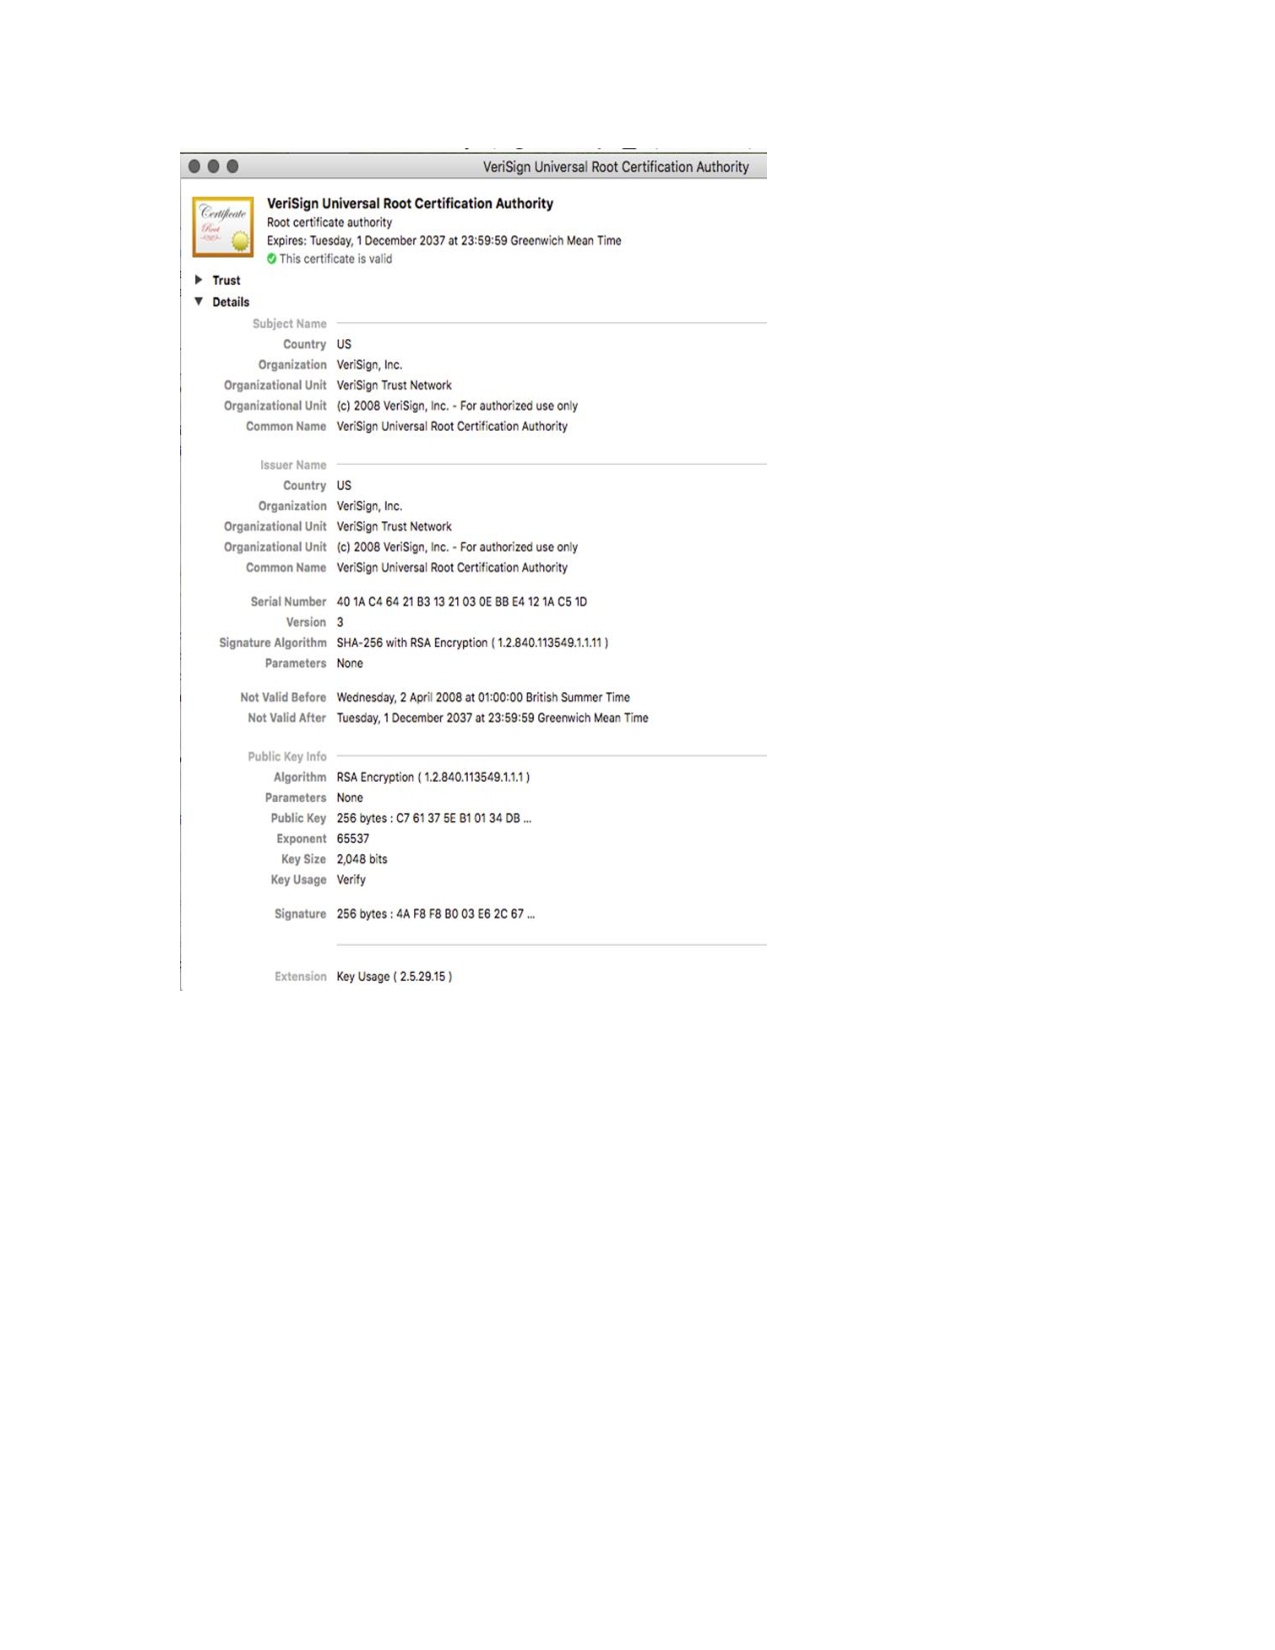
\includegraphics[width=0.85\columnwidth]{imagenes/certifverisignej.pdf}
\caption{El certificado de VeriSign (primeras líneas).}
\label{Fig.ejemplocertificadoVerisign}
\end{figure} 

Esta figura \ref{Fig.ejemplocertificadonAndroid}

\begin{figure}
\centering
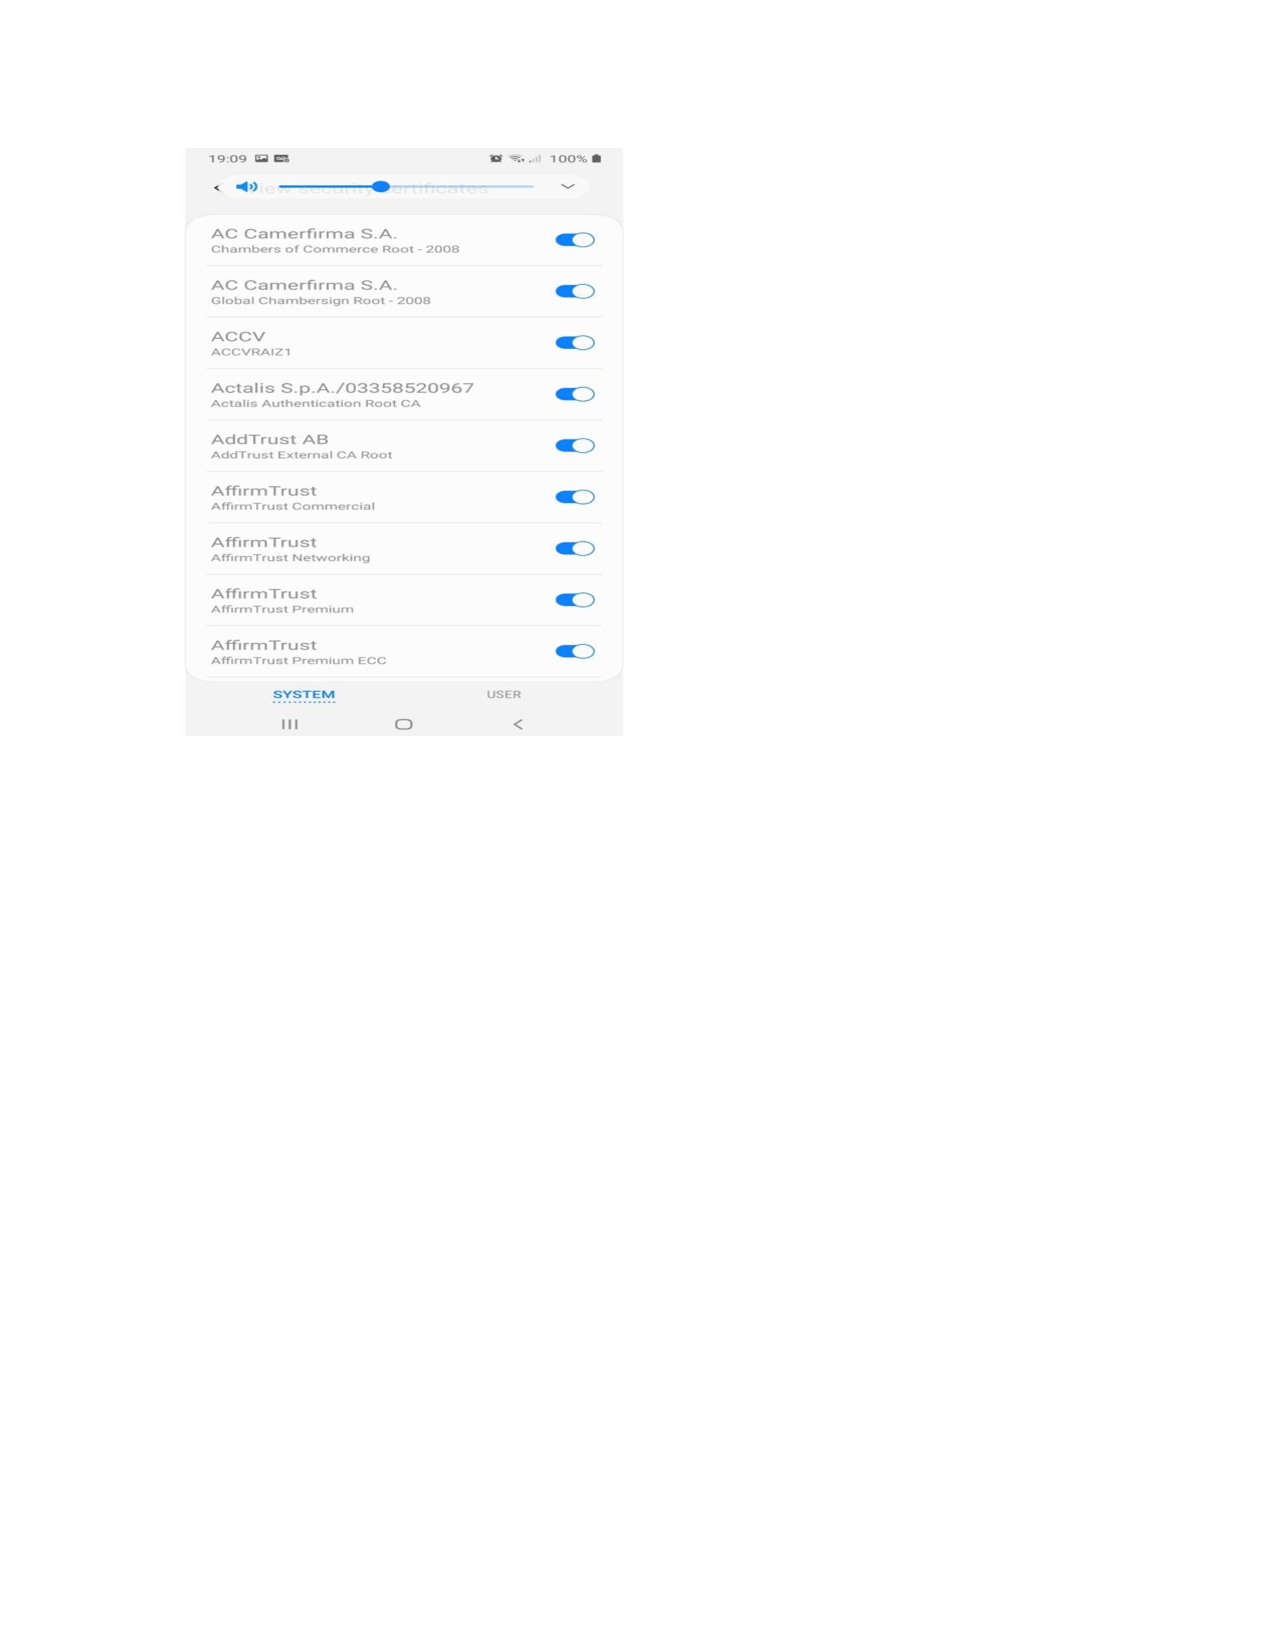
\includegraphics[width=0.85\columnwidth]{imagenes/certifenandroid.pdf}
\caption{Ejemplo de certificados cargados en un celular Andriod (1):}
\label{Fig.ejemplocertificadonAndroid}
\end{figure} 

Open settings -> Security-> Encryption \& Credentials” -> Certificates (para verlos, pero depende del modelo).
Fig. XX  Ejemplo de certificados cargados en un celuar Andriod (2)


Como explicaremos más adelante, existen programas que ayudan al usuario a crear un certificado y enviar la solicitud para que lo avale la empresa que él elija. Dichos programas dependen del sistema operativo que tenga la computadora del usuario, por ejemplo, en una computadora tipo Linux, existe el programa \textbf{openssl}.

La certificación de una llave cuesta dinero, su expedición es un negocio. Afortunadamente, la situación está cambiando, el \textit{Internet Security Research Group}  (ISRG) ha lanzado una iniciativa para expedir certificados gratuitamente.\footnote{See p732 (Ross Anderson Book)}  Cabe agregar que, en algunas situaciones (por ejemplo, para instalar algún software en una laptop), podemos usar un certificado no firmado. Existen programas que lo hacen:

Esta figura \ref{Fig.ejemplocertificadofirmadodueno}

\begin{figure}
\centering
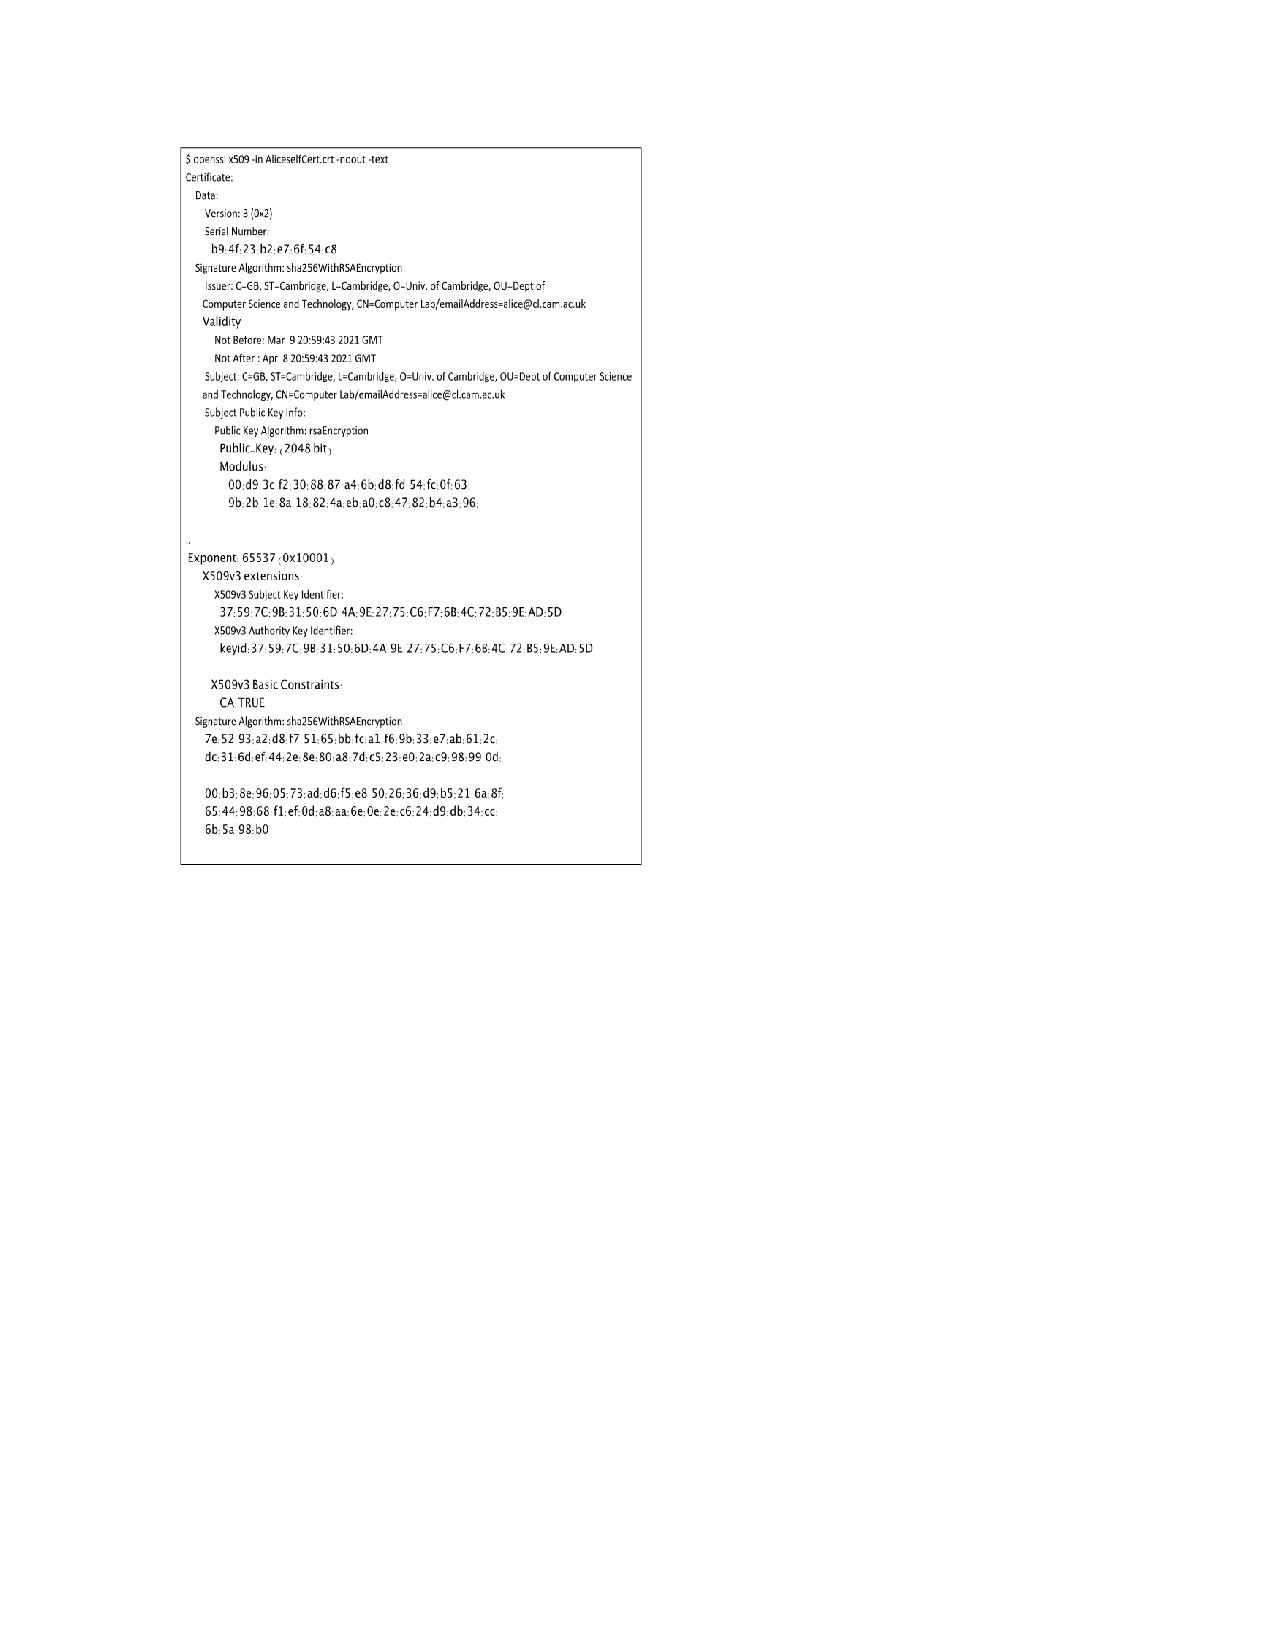
\includegraphics[width=0.85\columnwidth]{imagenes/certfirmadodueno.pdf}
\caption{Ejemplo de certificado (auto certificado) firmado por el dueño.}
\label{Fig.ejemplocertificadofirmadodueno}
\end{figure} 

Identidad e identidad digital
Falta

Esta figura \ref{Fig.Tablafirmas}

\begin{figure}
\centering
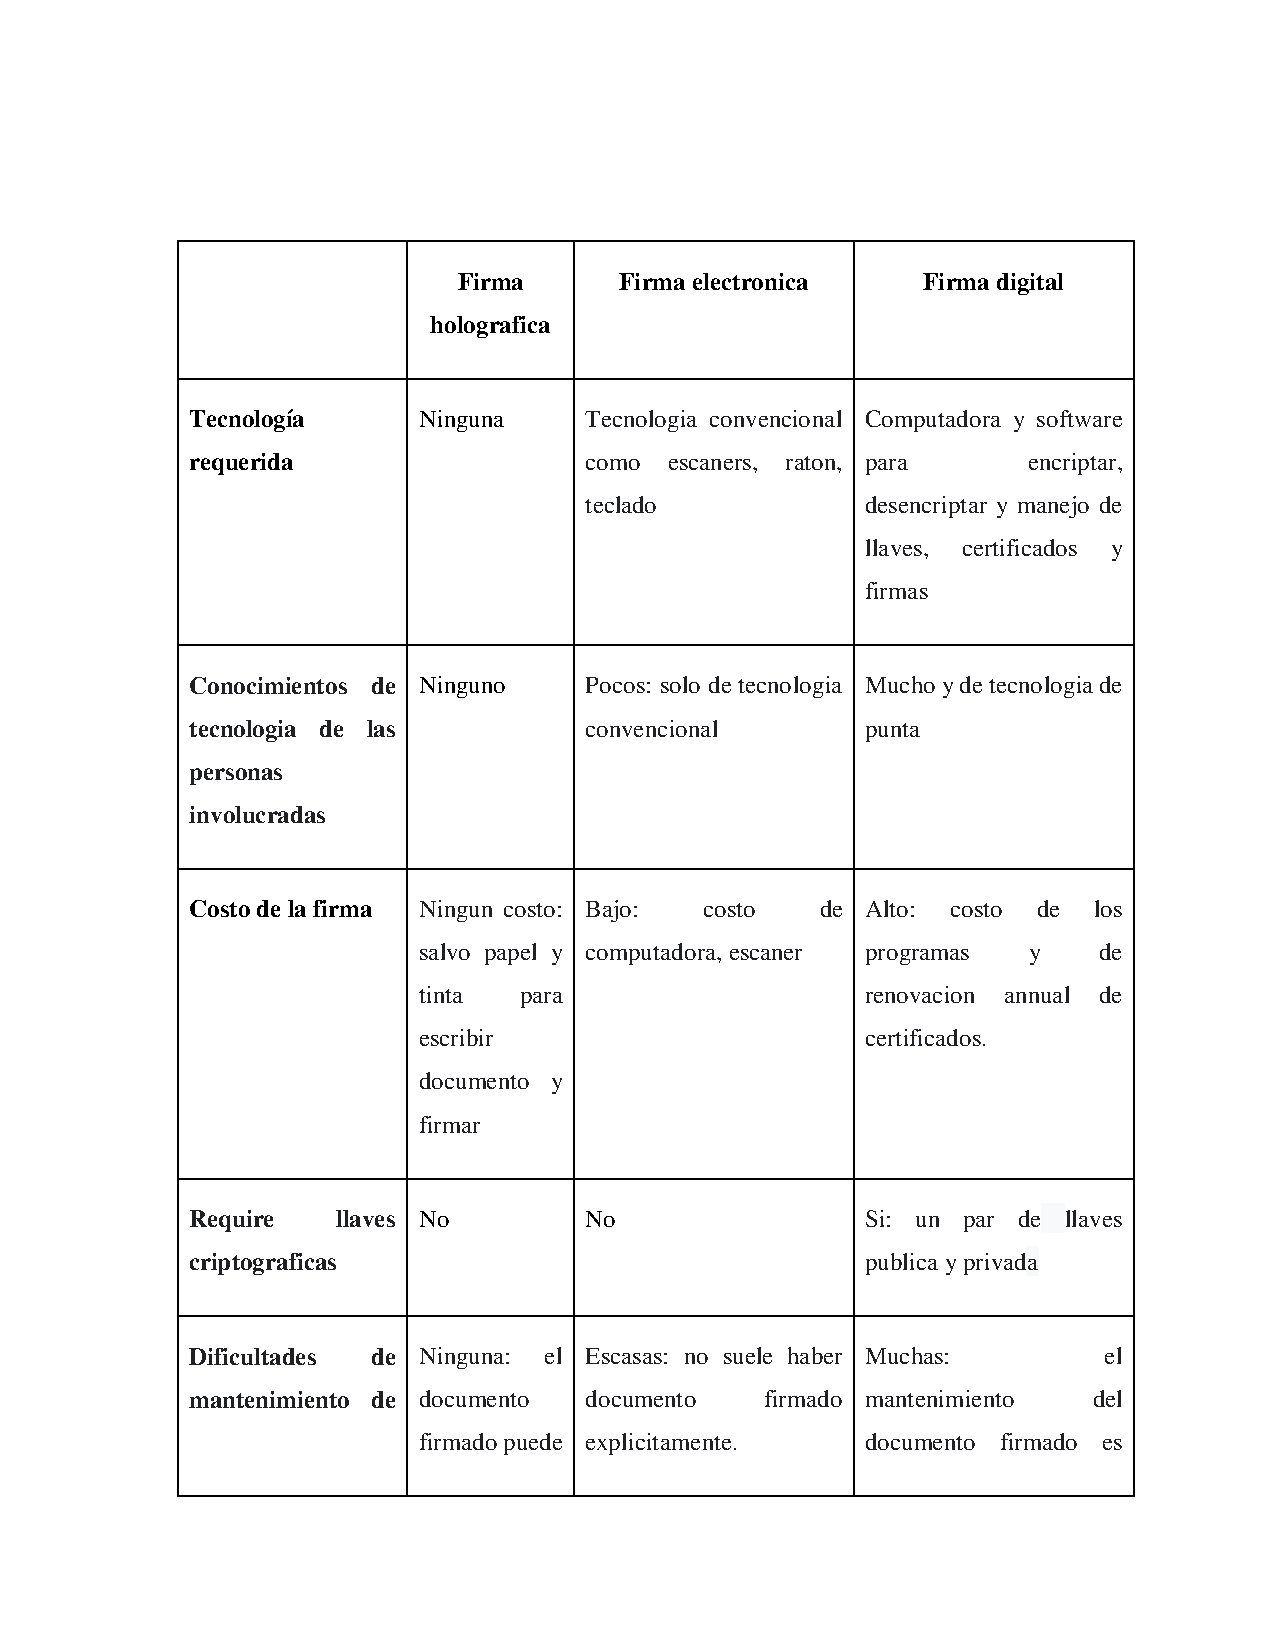
\includegraphics[width=0.85\columnwidth]{imagenes/tablafirmas.pdf}
\caption{Comparación jurídica de los tres tipos de firmas. }
\label{Fig.Tablafirmas}
\end{figure} 


























\chapter{cap perros }
\label{capcapperros}
.....

este cap de raton ...
\chapter{cap gatos}
\label{gatoigsa}
este cap de raton ...




%----------
%	Bibliography
%----------	

\clearpage
\addcontentsline{toc}{chapter}{Bibliography}
 

\printbibliography


%----------
%	Appendix
%----------	

% If your work includes Appendix, you can uncomment the following lines
%\chapter* {Appendix x}
%\pagenumbering{gobble} % Appendix pages are not numbered



%%\bibliographystyle{apalike}
%%\bibliography{referencias}

\end{document}